% Options for packages loaded elsewhere
% Options for packages loaded elsewhere
\PassOptionsToPackage{unicode}{hyperref}
\PassOptionsToPackage{hyphens}{url}
%
\documentclass[
]{scrreprt}
\usepackage{xcolor}
\usepackage{amsmath,amssymb}
\setcounter{secnumdepth}{2}
\usepackage{iftex}
\ifPDFTeX
  \usepackage[T1]{fontenc}
  \usepackage[utf8]{inputenc}
  \usepackage{textcomp} % provide euro and other symbols
\else % if luatex or xetex
  \usepackage{unicode-math} % this also loads fontspec
  \defaultfontfeatures{Scale=MatchLowercase}
  \defaultfontfeatures[\rmfamily]{Ligatures=TeX,Scale=1}
\fi
\usepackage{lmodern}
\ifPDFTeX\else
  % xetex/luatex font selection
\fi
% Use upquote if available, for straight quotes in verbatim environments
\IfFileExists{upquote.sty}{\usepackage{upquote}}{}
\IfFileExists{microtype.sty}{% use microtype if available
  \usepackage[]{microtype}
  \UseMicrotypeSet[protrusion]{basicmath} % disable protrusion for tt fonts
}{}
\usepackage{setspace}
\makeatletter
\@ifundefined{KOMAClassName}{% if non-KOMA class
  \IfFileExists{parskip.sty}{%
    \usepackage{parskip}
  }{% else
    \setlength{\parindent}{0pt}
    \setlength{\parskip}{6pt plus 2pt minus 1pt}}
}{% if KOMA class
  \KOMAoptions{parskip=half}}
\makeatother
% Make \paragraph and \subparagraph free-standing
\makeatletter
\ifx\paragraph\undefined\else
  \let\oldparagraph\paragraph
  \renewcommand{\paragraph}{
    \@ifstar
      \xxxParagraphStar
      \xxxParagraphNoStar
  }
  \newcommand{\xxxParagraphStar}[1]{\oldparagraph*{#1}\mbox{}}
  \newcommand{\xxxParagraphNoStar}[1]{\oldparagraph{#1}\mbox{}}
\fi
\ifx\subparagraph\undefined\else
  \let\oldsubparagraph\subparagraph
  \renewcommand{\subparagraph}{
    \@ifstar
      \xxxSubParagraphStar
      \xxxSubParagraphNoStar
  }
  \newcommand{\xxxSubParagraphStar}[1]{\oldsubparagraph*{#1}\mbox{}}
  \newcommand{\xxxSubParagraphNoStar}[1]{\oldsubparagraph{#1}\mbox{}}
\fi
\makeatother


\usepackage{longtable,booktabs,array}
\usepackage{calc} % for calculating minipage widths
\renewcommand{\arraystretch}{0.66} % reduce table line spacing
% Correct order of tables after \paragraph or \subparagraph
\usepackage{etoolbox}
\makeatletter
\patchcmd\longtable{\par}{\if@noskipsec\mbox{}\fi\par}{}{}
\makeatother
% Allow footnotes in longtable head/foot
\IfFileExists{footnotehyper.sty}{\usepackage{footnotehyper}}{\usepackage{footnote}}
\makesavenoteenv{longtable}
\usepackage{graphicx}
\makeatletter
\newsavebox\pandoc@box
\newcommand*\pandocbounded[1]{% scales image to fit in text height/width
  \sbox\pandoc@box{#1}%
  \Gscale@div\@tempa{\textheight}{\dimexpr\ht\pandoc@box+\dp\pandoc@box\relax}%
  \Gscale@div\@tempb{\linewidth}{\wd\pandoc@box}%
  \ifdim\@tempb\p@<\@tempa\p@\let\@tempa\@tempb\fi% select the smaller of both
  \ifdim\@tempa\p@<\p@\scalebox{\@tempa}{\usebox\pandoc@box}%
  \else\usebox{\pandoc@box}%
  \fi%
}
% Set default figure placement to htbp
\def\fps@figure{htbp}
\makeatother


% definitions for citeproc citations
\NewDocumentCommand\citeproctext{}{}
\NewDocumentCommand\citeproc{mm}{%
  \begingroup\def\citeproctext{#2}\cite{#1}\endgroup}
\makeatletter
 % allow citations to break across lines
 \let\@cite@ofmt\@firstofone
 % avoid brackets around text for \cite:
 \def\@biblabel#1{}
 \def\@cite#1#2{{#1\if@tempswa , #2\fi}}
\makeatother
\newlength{\cslhangindent}
\setlength{\cslhangindent}{1.5em}
\newlength{\csllabelwidth}
\setlength{\csllabelwidth}{3em}
\newenvironment{CSLReferences}[2] % #1 hanging-indent, #2 entry-spacing
 {\begin{list}{}{%
  \setlength{\itemindent}{0pt}
  \setlength{\leftmargin}{0pt}
  \setlength{\parsep}{0pt}
  \setlength{\baselineskip}{12pt}
  % turn on hanging indent if param 1 is 1
  \ifodd #1
   \setlength{\leftmargin}{\cslhangindent}
   \setlength{\itemindent}{-1\cslhangindent}
  \fi
  % set entry spacing
  \setlength{\itemsep}{4pt}}}
 {\end{list}}
\usepackage{calc}
\newcommand{\CSLBlock}[1]{\hfill\break\parbox[t]{\linewidth}{\strut\ignorespaces#1\strut}}
\newcommand{\CSLLeftMargin}[1]{\parbox[t]{\csllabelwidth}{\strut#1\strut}}
\newcommand{\CSLRightInline}[1]{\parbox[t]{\linewidth - \csllabelwidth}{\strut#1\strut}}
\newcommand{\CSLIndent}[1]{\hspace{\cslhangindent}#1}



\setlength{\emergencystretch}{3em} % prevent overfull lines

\providecommand{\tightlist}{%
  \setlength{\itemsep}{0pt}\setlength{\parskip}{0pt}}



 


\renewcommand{\chapterformat}{Chapter~\thechapter\autodot\enskip}
\renewcommand{\chaptermarkformat}{Chapter~\thechapter\autodot\enskip}
\usepackage{fontspec}
\setmainfont{Arial}
\setsansfont{Arial}
\usepackage{anyfontsize}
\fontsize{11}{16}\selectfont
\usepackage{etoolbox}
\AtBeginEnvironment{tabular}{\vspace{12pt}\small}
\AtBeginEnvironment{longtable}{\vspace{12pt}\small}
\usepackage{booktabs}
\usepackage{graphicx}
\usepackage[nottoc,notlof,notlot]{tocbibind}
\PassOptionsToPackage{table}{xcolor}
\usepackage{xcolor}
\renewcommand{\bibsection}{}
\usepackage[a4paper, top=2cm, bottom=3cm, left=2.5cm, right=2.5cm]{geometry}
\usepackage{tocloft}
\setcounter{tocdepth}{2}
\setlength{\cftbeforetoctitleskip}{0pt}
\setlength{\cftbeforeloftitleskip}{0pt}
\setlength{\cftbeforelottitleskip}{0pt}
\setlength{\cftaftertoctitleskip}{1pt}
\setlength{\cftafterloftitleskip}{1pt}
\setlength{\cftafterlottitleskip}{1pt}
\renewcommand{\cftsecleader}{\cftdotfill{\cftdotsep}}
\usepackage[all]{nowidow}
\usepackage{scrhack}
\usepackage{caption}
\captionsetup[figure]{font={footnotesize}, labelfont={bf}}
\captionsetup[table]{font={footnotesize}, labelfont={bf}}
\captionsetup[sfig]{font={footnotesize}, labelfont={bf}}
\DeclareCaptionLabelFormat{sfiglabelformat}{#1#2}
\captionsetup[sfig]{labelformat=sfiglabelformat, labelsep=colon}
\AtBeginDocument{\renewcommand{\thesfig}{\arabic{sfig}}}
\captionsetup[stbl]{font={footnotesize}, labelfont={bf}}
\DeclareCaptionLabelFormat{stbllabelformat}{#1#2}
\captionsetup[stbl]{labelformat=stbllabelformat, labelsep=colon}
\AtBeginDocument{\renewcommand{\thestbl}{\arabic{stbl}}}
\renewcommand{\theequation}{\arabic{equation}}
\counterwithout{equation}{chapter}
\usepackage{chngcntr}
\counterwithout{figure}{chapter}
\counterwithout{table}{chapter}
\usepackage{xurl}
\makeatletter
\renewcommand{\thechapter}{}
\renewcommand{\thesection}{\arabic{chapter}.\arabic{section}}
\renewcommand{\chapterformat}{}
\patchcmd{\chapter}{\if@openright\cleardoublepage\else\clearpage\fi}{}{}{}
\patchcmd{\@starttoc}{\begin{center}}{}{}{}
\makeatother
\RedeclareSectionCommand[ beforeskip=6pt plus 1pt minus 1pt, afterskip=1pt plus 1pt minus 1pt, font=\fontsize{16pt}{18pt}\bfseries\sffamily, ]{chapter}
\RedeclareSectionCommand[ beforeskip=4pt plus 1pt minus 1pt, afterskip=1pt plus 1pt minus 1pt, font=\fontsize{14pt}{16pt}\bfseries\sffamily, ]{section}
\RedeclareSectionCommand[ beforeskip=3pt plus 1pt minus 1pt, afterskip=1pt plus 1pt minus 1pt, font=\fontsize{12pt}{14pt}\bfseries\sffamily, ]{subsection}
\RedeclareSectionCommand[ beforeskip=2pt plus 1pt minus 1pt, afterskip=1pt plus 1pt minus 1pt, font=\fontsize{11pt}{12pt}\bfseries\sffamily, ]{subsubsection}
\RedeclareSectionCommand[ beforeskip=1pt plus 1pt minus 1pt, afterskip=1pt plus 1pt minus 1pt, font=\fontsize{11pt}{12pt}\bfseries\sffamily, ]{paragraph}
\RedeclareSectionCommand[ beforeskip=1pt plus 1pt minus 1pt, afterskip=1pt plus 1pt minus 1pt, font=\fontsize{11pt}{12pt}\bfseries\sffamily, ]{subparagraph}
\makeatletter
\@ifpackageloaded{float}{}{\usepackage{float}}
\floatstyle{plain}
\@ifundefined{c@chapter}{\newfloat{con}{h}{locon}}{\newfloat{con}{h}{locon}[chapter]}
\floatname{con}{Contact}
\newcommand*\listofcons{\listof{con}{List of Contacts}}
\makeatother
\makeatletter
\@ifpackageloaded{float}{}{\usepackage{float}}
\floatstyle{plain}
\@ifundefined{c@chapter}{\newfloat{sfig}{h}{losfig}}{\newfloat{sfig}{h}{losfig}[chapter]}
\floatname{sfig}{Figure S}
\newcommand*\quartosfigref[1]{Figure \hyperref[#1]{S\ref{#1}}}
\@ifpackageloaded{caption}{}{\usepackage{caption}}
\DeclareCaptionLabelFormat{quartosfigreflabelformat}{#1#2}
\captionsetup[sfig]{labelformat=quartosfigreflabelformat}
\newcommand*\listofsfigs{\listof{sfig}{List of List of Supplementary Figuress}}
\makeatother
\makeatletter
\@ifpackageloaded{float}{}{\usepackage{float}}
\floatstyle{plain}
\@ifundefined{c@chapter}{\newfloat{stbl}{h}{lostbl}}{\newfloat{stbl}{h}{lostbl}[chapter]}
\floatname{stbl}{Table S}
\floatstyle{plaintop}
\restylefloat{stbl}
\newcommand*\quartostblref[1]{Table \hyperref[#1]{S\ref{#1}}}
\@ifpackageloaded{caption}{}{\usepackage{caption}}
\DeclareCaptionLabelFormat{quartostblreflabelformat}{#1#2}
\captionsetup[stbl]{labelformat=quartostblreflabelformat}
\newcommand*\listofstbls{\listof{stbl}{List of List of Supplementary Tabless}}
\makeatother
\makeatletter
\@ifpackageloaded{caption}{}{\usepackage{caption}}
\AtBeginDocument{%
\ifdefined\contentsname
  \renewcommand*\contentsname{Table of contents}
\else
  \newcommand\contentsname{Table of contents}
\fi
\ifdefined\listfigurename
  \renewcommand*\listfigurename{List of Figures}
\else
  \newcommand\listfigurename{List of Figures}
\fi
\ifdefined\listtablename
  \renewcommand*\listtablename{List of Tables}
\else
  \newcommand\listtablename{List of Tables}
\fi
\ifdefined\figurename
  \renewcommand*\figurename{Figure}
\else
  \newcommand\figurename{Figure}
\fi
\ifdefined\tablename
  \renewcommand*\tablename{Table}
\else
  \newcommand\tablename{Table}
\fi
}
\@ifpackageloaded{float}{}{\usepackage{float}}
\floatstyle{ruled}
\@ifundefined{c@chapter}{\newfloat{codelisting}{h}{lop}}{\newfloat{codelisting}{h}{lop}[chapter]}
\floatname{codelisting}{Listing}
\newcommand*\listoflistings{\listof{codelisting}{List of Listings}}
\makeatother
\makeatletter
\makeatother
\makeatletter
\@ifpackageloaded{caption}{}{\usepackage{caption}}
\@ifpackageloaded{subcaption}{}{\usepackage{subcaption}}
\makeatother
\usepackage{bookmark}
\IfFileExists{xurl.sty}{\usepackage{xurl}}{} % add URL line breaks if available
\urlstyle{same}
\hypersetup{
  pdfauthor={Robin Pfaff},
  hidelinks,
  pdfcreator={LaTeX via pandoc}}


\author{Robin Pfaff}
\date{2025-12}
\begin{document}

\begin{titlepage}
    \centering
    \vspace*{2cm}
    {\fontsize{18}{22}\bfseries In-situ aerial mapping of New Zealand Myrtaceae affected by Myrtle Rust (\textit{Austropuccinia psidii}) using deep learning\par}
    \vspace{5.5cm}
    {\fontsize{12}{14}\bfseries by\par}
    {\fontsize{12}{14}\bfseries Robin Pfaff\par}
    {\fontsize{12}{14}\selectfont 2026\par}
    \vspace{5cm}
    {\fontsize{12}{14}\bfseries School of Science\par}
    \vspace{1.5cm}
    {\fontsize{12}{14}\selectfont A thesis submitted to Auckland University of Technology in partial fulfilment
of the requirements for the degree of Master of Science (Research) - Geospatial Science\par}
    \vfill
    \begin{flushleft}
        Supervisors:\\
        - Dr. Rebecca Rogers\\
        - Graham Hinchliffe
    \end{flushleft}
\end{titlepage}

\clearpage
\pagenumbering{arabic}
\setcounter{page}{2}

\thispagestyle{empty}
\vspace*{\fill}

\noindent{\Large\textbf{Imprint}}

\vspace{0.5cm}

\noindent\textbf{Form of citation}\\
APA 7th edition

\noindent\textbf{Keywords}\\
Myrtle Rust, \textit{Austropuccinia psidii}, \textit{Syzygium maire}, Deep Learning, LiDAR, Multispectral, High-Resolution UAV-imagery
\newpage


\setstretch{1.5}
\chapter*{Abstract}\label{abstract}

Invasive fungal pathogens pose a significant threat to forest ecosystems
worldwide and have far-reaching consequences for tree species. The rust
fungus (\emph{Austropuccinia psidii}) causes the disease commonly known
as myrtle rust and threatens susceptible Myrtaceae populations on
several continents. This includes \emph{Syzygium maire}, a rare taonga
(treasure) species endemic to New Zealand that is significant in Māori
culture and ecologically important, but is now threatened with
extinction. Accurate spatial mapping of threatened populations is
essential for targeted management and conservation efforts, but
traditional ground-based survey methods are logistically challenging and
time-consuming.

The practical application of unmanned aerial vehicles (UAVs) in
combination with deep learning was evaluated to detect \emph{S. maire}
in dense, species-rich native forests. High-resolution RGB (1.5 cm) and
multispectral (2.5 cm) imagery were captured from four urban forest
reserves on New Zealand's North Island using consumer-grade imaging
sensors. A fully convolutional neural network for semantic segmentation
(U-Net) was trained to classify \emph{S. maire} from background
vegetation. Furthermore, dataset composition and hyperparameter
configurations were systematically tested including loss functions,
learning rates, and different spectral band combinations. Point cloud
segmentation approaches using a UAV-mounted LiDAR system were also
qualitatively evaluated to assess the potential for three-dimensional
tree instance detection.

Site-specific models showed moderate to good detection performance (F1
scores: 0.46--0.81), with RGB images performing comparably or marginally
better than multispectral images. Dice loss outperformed pixel-wise
approaches in handling severe class imbalances, and an aggressive
learning rate of 0.02 with adaptive scheduling led to significantly
better performance. However, generalising models across multiple sites
proved more difficult due to site-specific differences (best F1=0.51).
LiDAR-based instance segmentation algorithms developed for managed
forests have potential for the dense, structurally complex context of
natural forests, but are insufficient without further development.

The results show that deep learning can successfully identify \emph{S.
maire} under optimal, site-specific conditions. At the same time,
critical limitations for operational real-world use were identified. The
limited availability of training samples, the severe class imbalance of
3.4±0.7\% (mean±SE) target class and the insufficient radiometric
calibration capabilities of low-cost multispectral sensors fundamentally
limit the approach. These findings highlight the need for standardised
frameworks governing multispectral data capture and radiometric
calibration.

The findings expose significant challenges in translating remote sensing
methods from simplified scenarios to operational conservation monitoring
in structurally complex forests. The methodological insights regarding
hyperparameter optimisation, spectral band selection, and calibration
challenges can be transferred to analogous applications for species
detection. As invasive pathogens increasingly threaten forest
biodiversity worldwide, the development of robust detection methods for
(rare) species in complex environments remains essential to support
proactive conservation and biosecurity measures.

\newpage

\chapter*{Attestation of Authorship}\label{attestation-of-authorship}

I hereby declare that this submission is my own work and that, to the
best of my knowledge and belief, it contains no material previously
published or written by another person (except where explicitly defined
in the acknowledgements), nor used artificial intelligence tools or
generative artificial intelligence tools (unless it is clearly stated
and referenced, along with the purpose of use), nor material which to a
substantial extent has been submitted for the award of any other degree
or diploma of a university or other institution of higher learning.

\vspace{0.5cm}

Signed:

\pandocbounded{\includegraphics[keepaspectratio]{../2_1_figures/Unterschrift_Robin_Pfaff.png}}

Robin Pfaff

Date: 19/02/2026

\vspace{2cm}

\chapter*{Statement of Contribution}\label{statement-of-contribution}

All data collection, processing, and analysis were completed by R.P.,
with assistance from G.H. and R.R. during UAV operations; initial LiDAR
data processing was completed by G.H., with further processing and
analysis by R.P. The thesis was written by R.P., with feedback from R.R.
and G.H.

\newpage

\chapter*{Acknowledgements}\label{acknowledgements}

I would like to thank the following people who provided guidance and
support during this thesis project. My supervisors, Dr.~Rebecca Rogers
and Graham Hinchliffe, for their continuous feedback, support, and
encouragement throughout the project, especially for the open and
uncomplicated communication. I would also like to thank Derek Craig
(formerly of \href{https://kaipatiki.org.nz}{Kaipātiki Project}) for
initial guidance on site selection, and Maria Valkova
(\href{https://kaipatiki.org.nz}{Kaipātiki Project}), Kathy McCormack
(Friends of Bushglen Reserve), and Robert Beresford (Bioeconomy Science
Institute) for directing me to the \emph{S. maire} during fieldwork and
providing me with valuable contextual information around \emph{S.
maire}. I would also like to thank Jamie Chapman and Andrea Campos, not
only for their help with UAV operations, but also for their ongoing
mental support. Furthermore, I would like to thank Laurin Frey for his
help with proofreading and feedback. Finally, and most of all, I would
like to thank my Godmother (Therese Rudolph von Rohr) and my parents
(Doris and René Pfaff) without whom I would not have been able to
realise my dream of pursuing a Master's degree in beautiful Aotearoa.

\newpage

\listoffigures

\newpage

\listoftables

\newpage

\tableofcontents

\newpage

\chapter{Chapter 1 Introduction}\label{sec-introduction}

\section{Global Emergence and Spread of Myrtle
Rust}\label{global-emergence-and-spread-of-myrtle-rust}

The spread of invasive fungal pathogens is increasingly impacting forest
ecosystems worldwide, with their dispersion to new areas partially
facilitated by ever-increasing global trade and travel
(\citeproc{ref-grgurinovicEucalyptusrust2006}{Grgurinovic et al., 2006};
\citeproc{ref-paapInvasionFrameworks2022}{Paap et al., 2022};
\citeproc{ref-wingfieldunifiedframework2017}{Wingfield et al., 2017}).
Rust fungi belong to the diverse phylum Basidiomycota and are biotrophic
plant parasites (\citeproc{ref-helferRustfungi2014}{Helfer, 2014}). One
member of the rust fungi, \hyperref[acronyms_AP]{\emph{Austropuccinia
psidii}}, formerly \emph{Puccinia psidii}
(\citeproc{ref-beenkenAustropuccinianew2017}{Beenken, 2017}), has a
broad host range outside its native habitat. Originating from South and
Central America, one biotype of this fungus is considered pandemic and
spread to Hawaii, Australia, Southeast Asia, China, Japan, and New
Zealand (\citeproc{ref-duplessispandemicstrain2019}{Du Plessis et al.,
2019}; \citeproc{ref-granadospandemicbiotype2017}{Granados et al.,
2017}; \citeproc{ref-stewartGeneticdiversity2018}{Stewart et al.,
2018}). Globally, \hyperref[acronyms_AP]{\emph{A. psidii}} infects
approximately 480 Myrtaceae species
(\citeproc{ref-soewartoj.Austropucciniapsidii2019}{Soewarto et al.,
2019}), causing the disease commonly known as
\hyperref[acronyms_MR]{myrtle rust}. Due to the lack of co-evolution,
Oceanic Myrtaceae did not have the opportunity to adapt to
\hyperref[acronyms_MR]{myrtle rust}, making them epidemiologically naïve
to the pathogen and, as a result, more susceptible
(\citeproc{ref-makinsonMyrtleRust2018}{Makinson, 2018}). Whilst it is
thought that \hyperref[acronyms_AP]{\emph{A. psidii}} has arrived in New
Zealand in 2017 via wind, its urediniospores can also spread by humans,
birds or insects (\citeproc{ref-magyarDispersalStrategies2016}{Magyar et
al., 2016}; \citeproc{ref-schmidShortCommunication2021}{Schmid et al.,
2021}).

\section{Plant-level Symptoms of Myrtle
Rust}\label{plant-level-symptoms-of-myrtle-rust}

\hyperref[acronyms_AP]{\emph{A. psidii}} spores infect the host-plant
only on actively growing tissue like young shoots, developing leaves and
fruits (\citeproc{ref-boufleurDiagnosticGuide2023}{Boufleur et al.,
2023}; \citeproc{ref-chockglobalthreat2020}{Chock, 2020};
\citeproc{ref-glenPucciniapsidii2007}{Glen et al., 2007}). After
germination and a latent period of approximately two weeks, the symptoms
start to show (Figure~\ref{fig-symptoms}; Beresford et al., 2020).
Initially, the growing uredinial spores form yellow pustules
(Figure~\ref{fig-pustules}). These growth areas turn into red blotches
on leaves, killing the photosynthetic tissue and preventing the growth
of new meristematic tissue, leading to the death of shoot tips
(Figure~\ref{fig-red_blotches}) and flowers. Sustained infection
ultimately leads to substantial defoliation
(Figure~\ref{fig-smaire_stand}; Boufleur et al., 2023). Hence, infection
hinders the host to produce new photosynthetic tissue and development of
seeds, disrupting the reproductive cycle
(\citeproc{ref-fenshamUnprecedentedextinction2021}{Fensham \&
Radford-Smith, 2021}). In severe cases, sustained tissue loss and
inability to produce new seeds can render the host infertile, ultimately
leading to mortality
(\citeproc{ref-fenshamUnprecedentedextinction2021}{Fensham \&
Radford-Smith, 2021}). Even when seed production is not entirely
suppressed and seedlings germinate, they are highly susceptible to
infection, severely limiting regeneration
(\citeproc{ref-fernandez-winzerDirectindirect2020}{Fernandez-Winzer et
al., 2020}). Such reproduction failure has raised concerns that highly
susceptible species may face extinction within a single generation
(\citeproc{ref-carnegieImpactinvasive2016}{Carnegie et al., 2016};
\citeproc{ref-fenshamUnprecedentedextinction2021}{Fensham \&
Radford-Smith, 2021}). As a consequence, this may have cascading effects
across trophic levels, impacting birds, insects, and other organisms
that depend on these species as habitat or food
(\citeproc{ref-sutherlandMonitoringAustropuccinia2020}{Sutherland et
al., 2020}).

\begin{figure}

\centering{

\begin{figure}[H]

\begin{minipage}{0.49\linewidth}

\centering{

\pandocbounded{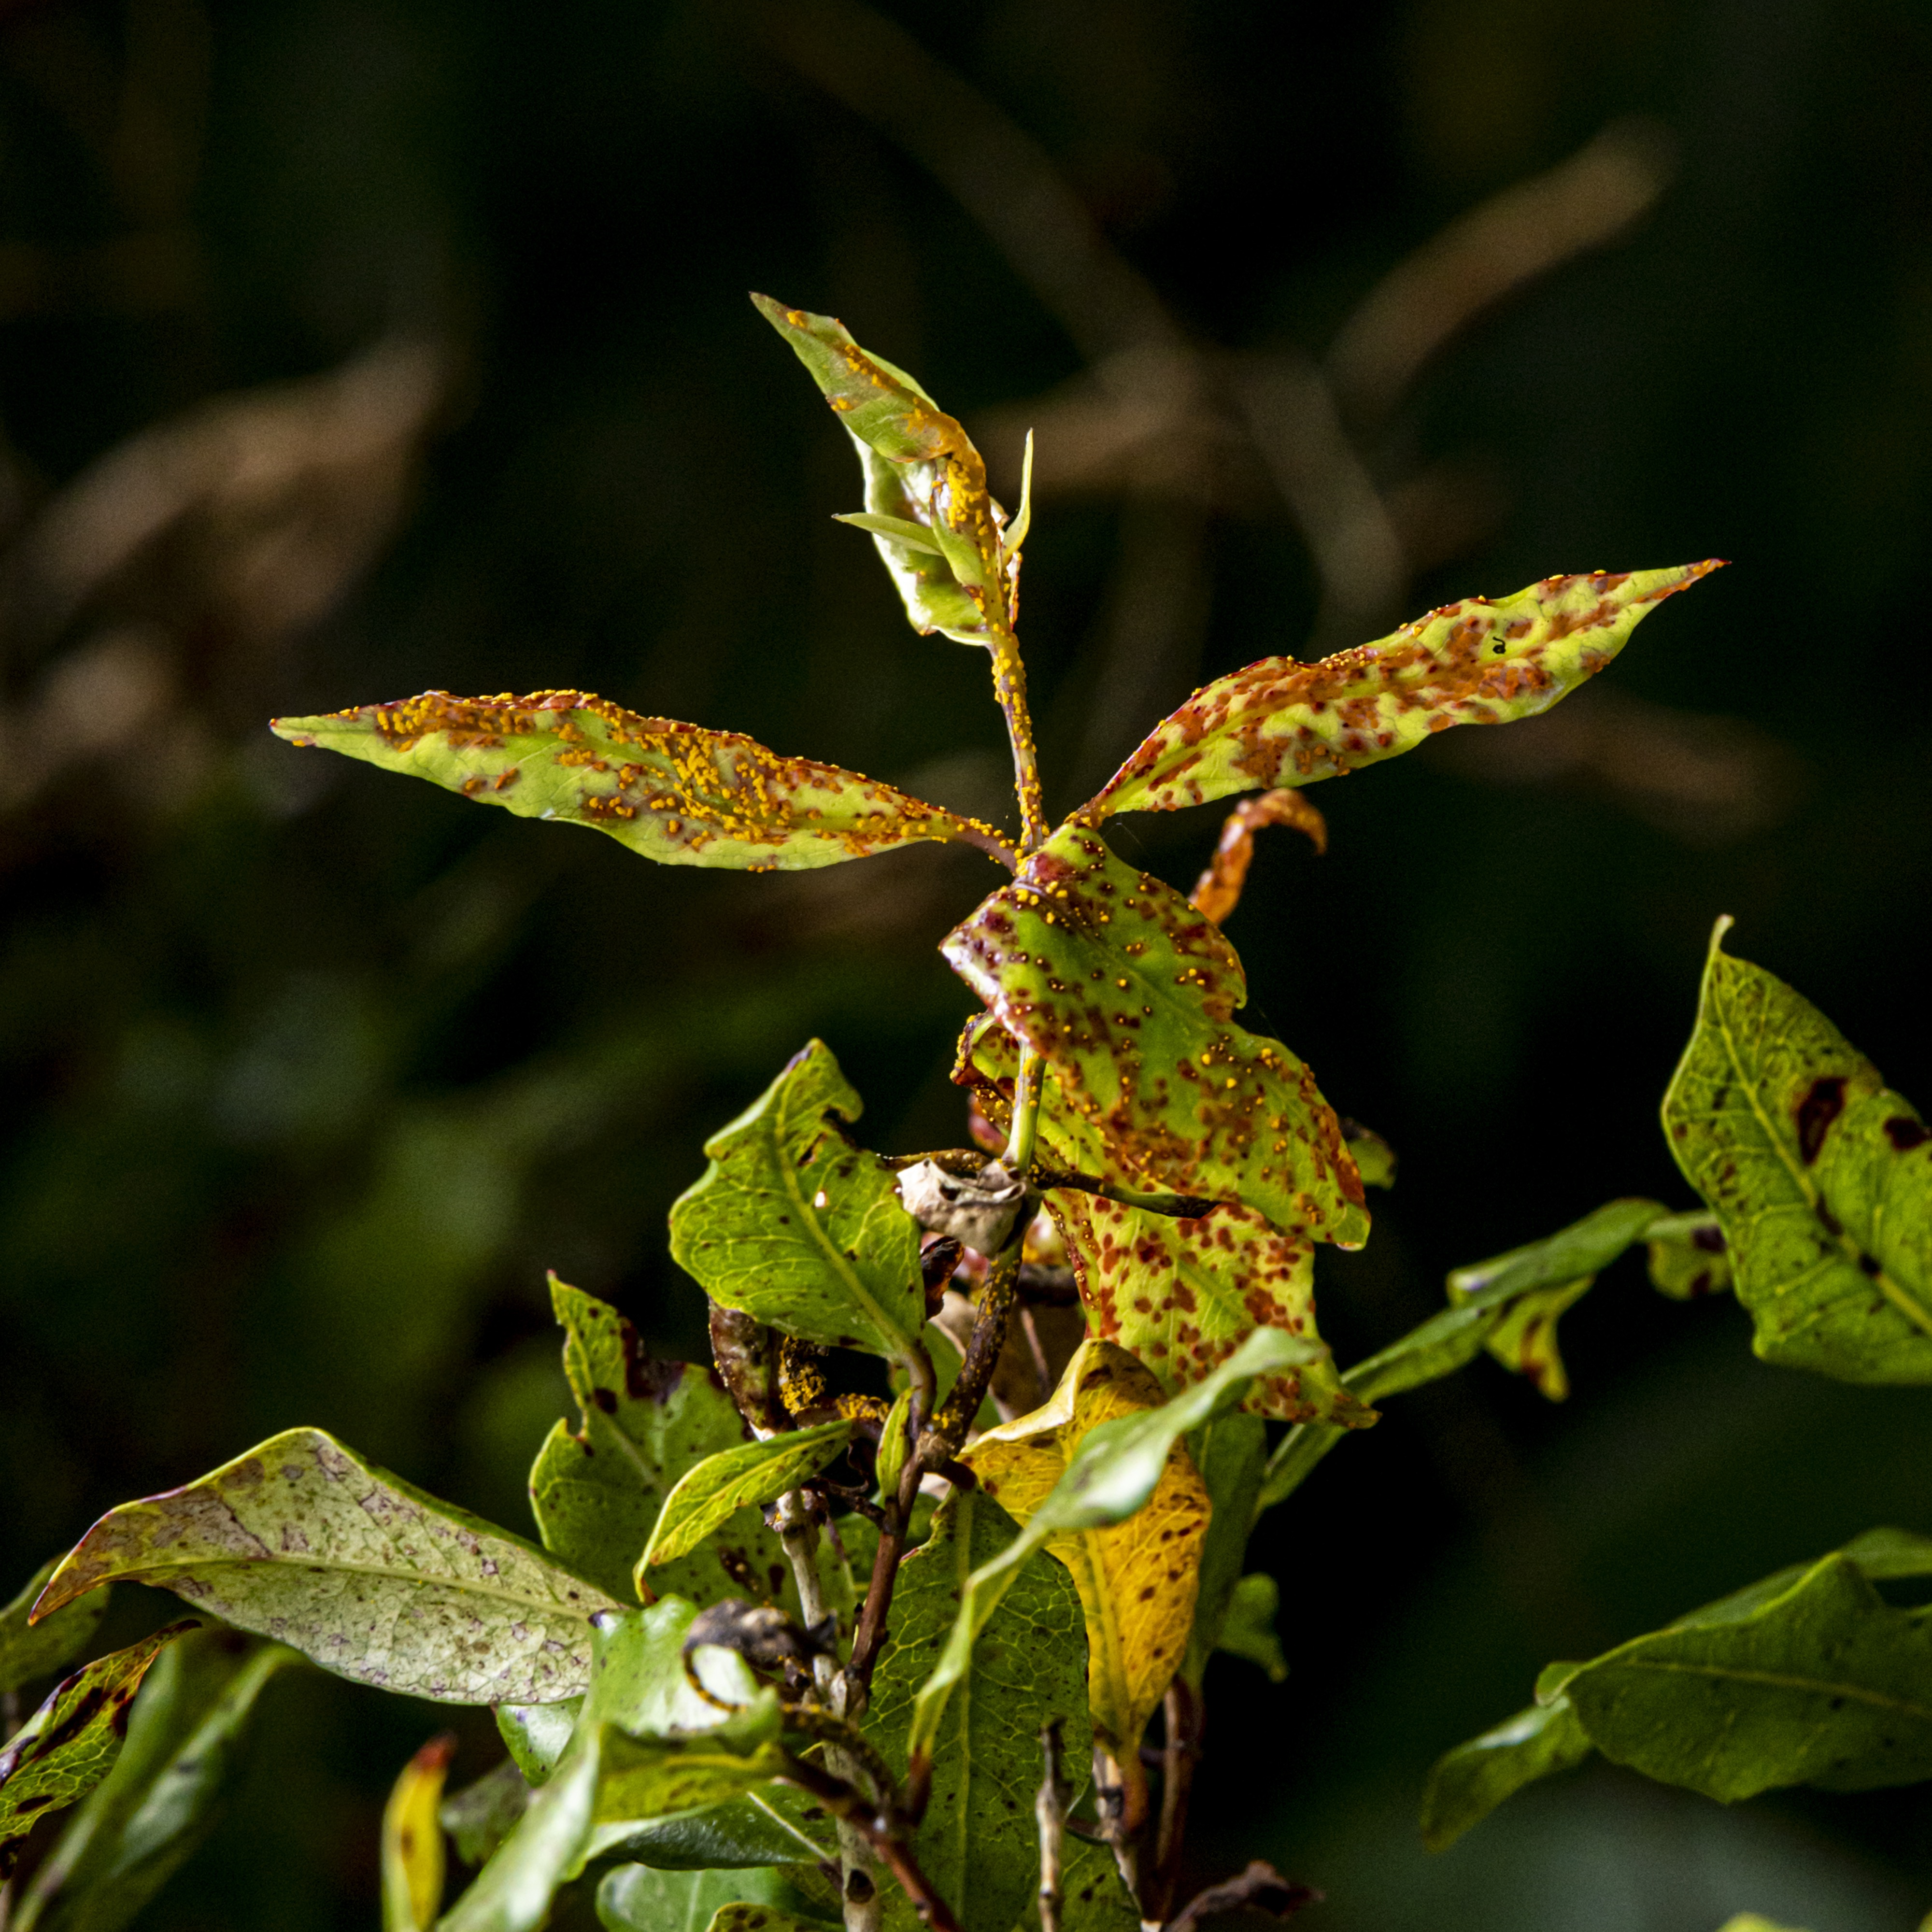
\includegraphics[keepaspectratio]{../2_1_figures/introduction/PFR/Myrtle Rust- Native Swamp Maire Tree _PFR2575-2.jpg}}

}

\subcaption{\label{fig-pustules}Yellow pustules on leaves. Image:
Copyright by Bioeconomy Science Institute. Reprinted with permission.}

\end{minipage}%
%
\begin{minipage}{0.02\linewidth}
~\end{minipage}%
%
\begin{minipage}{0.49\linewidth}

\centering{

\pandocbounded{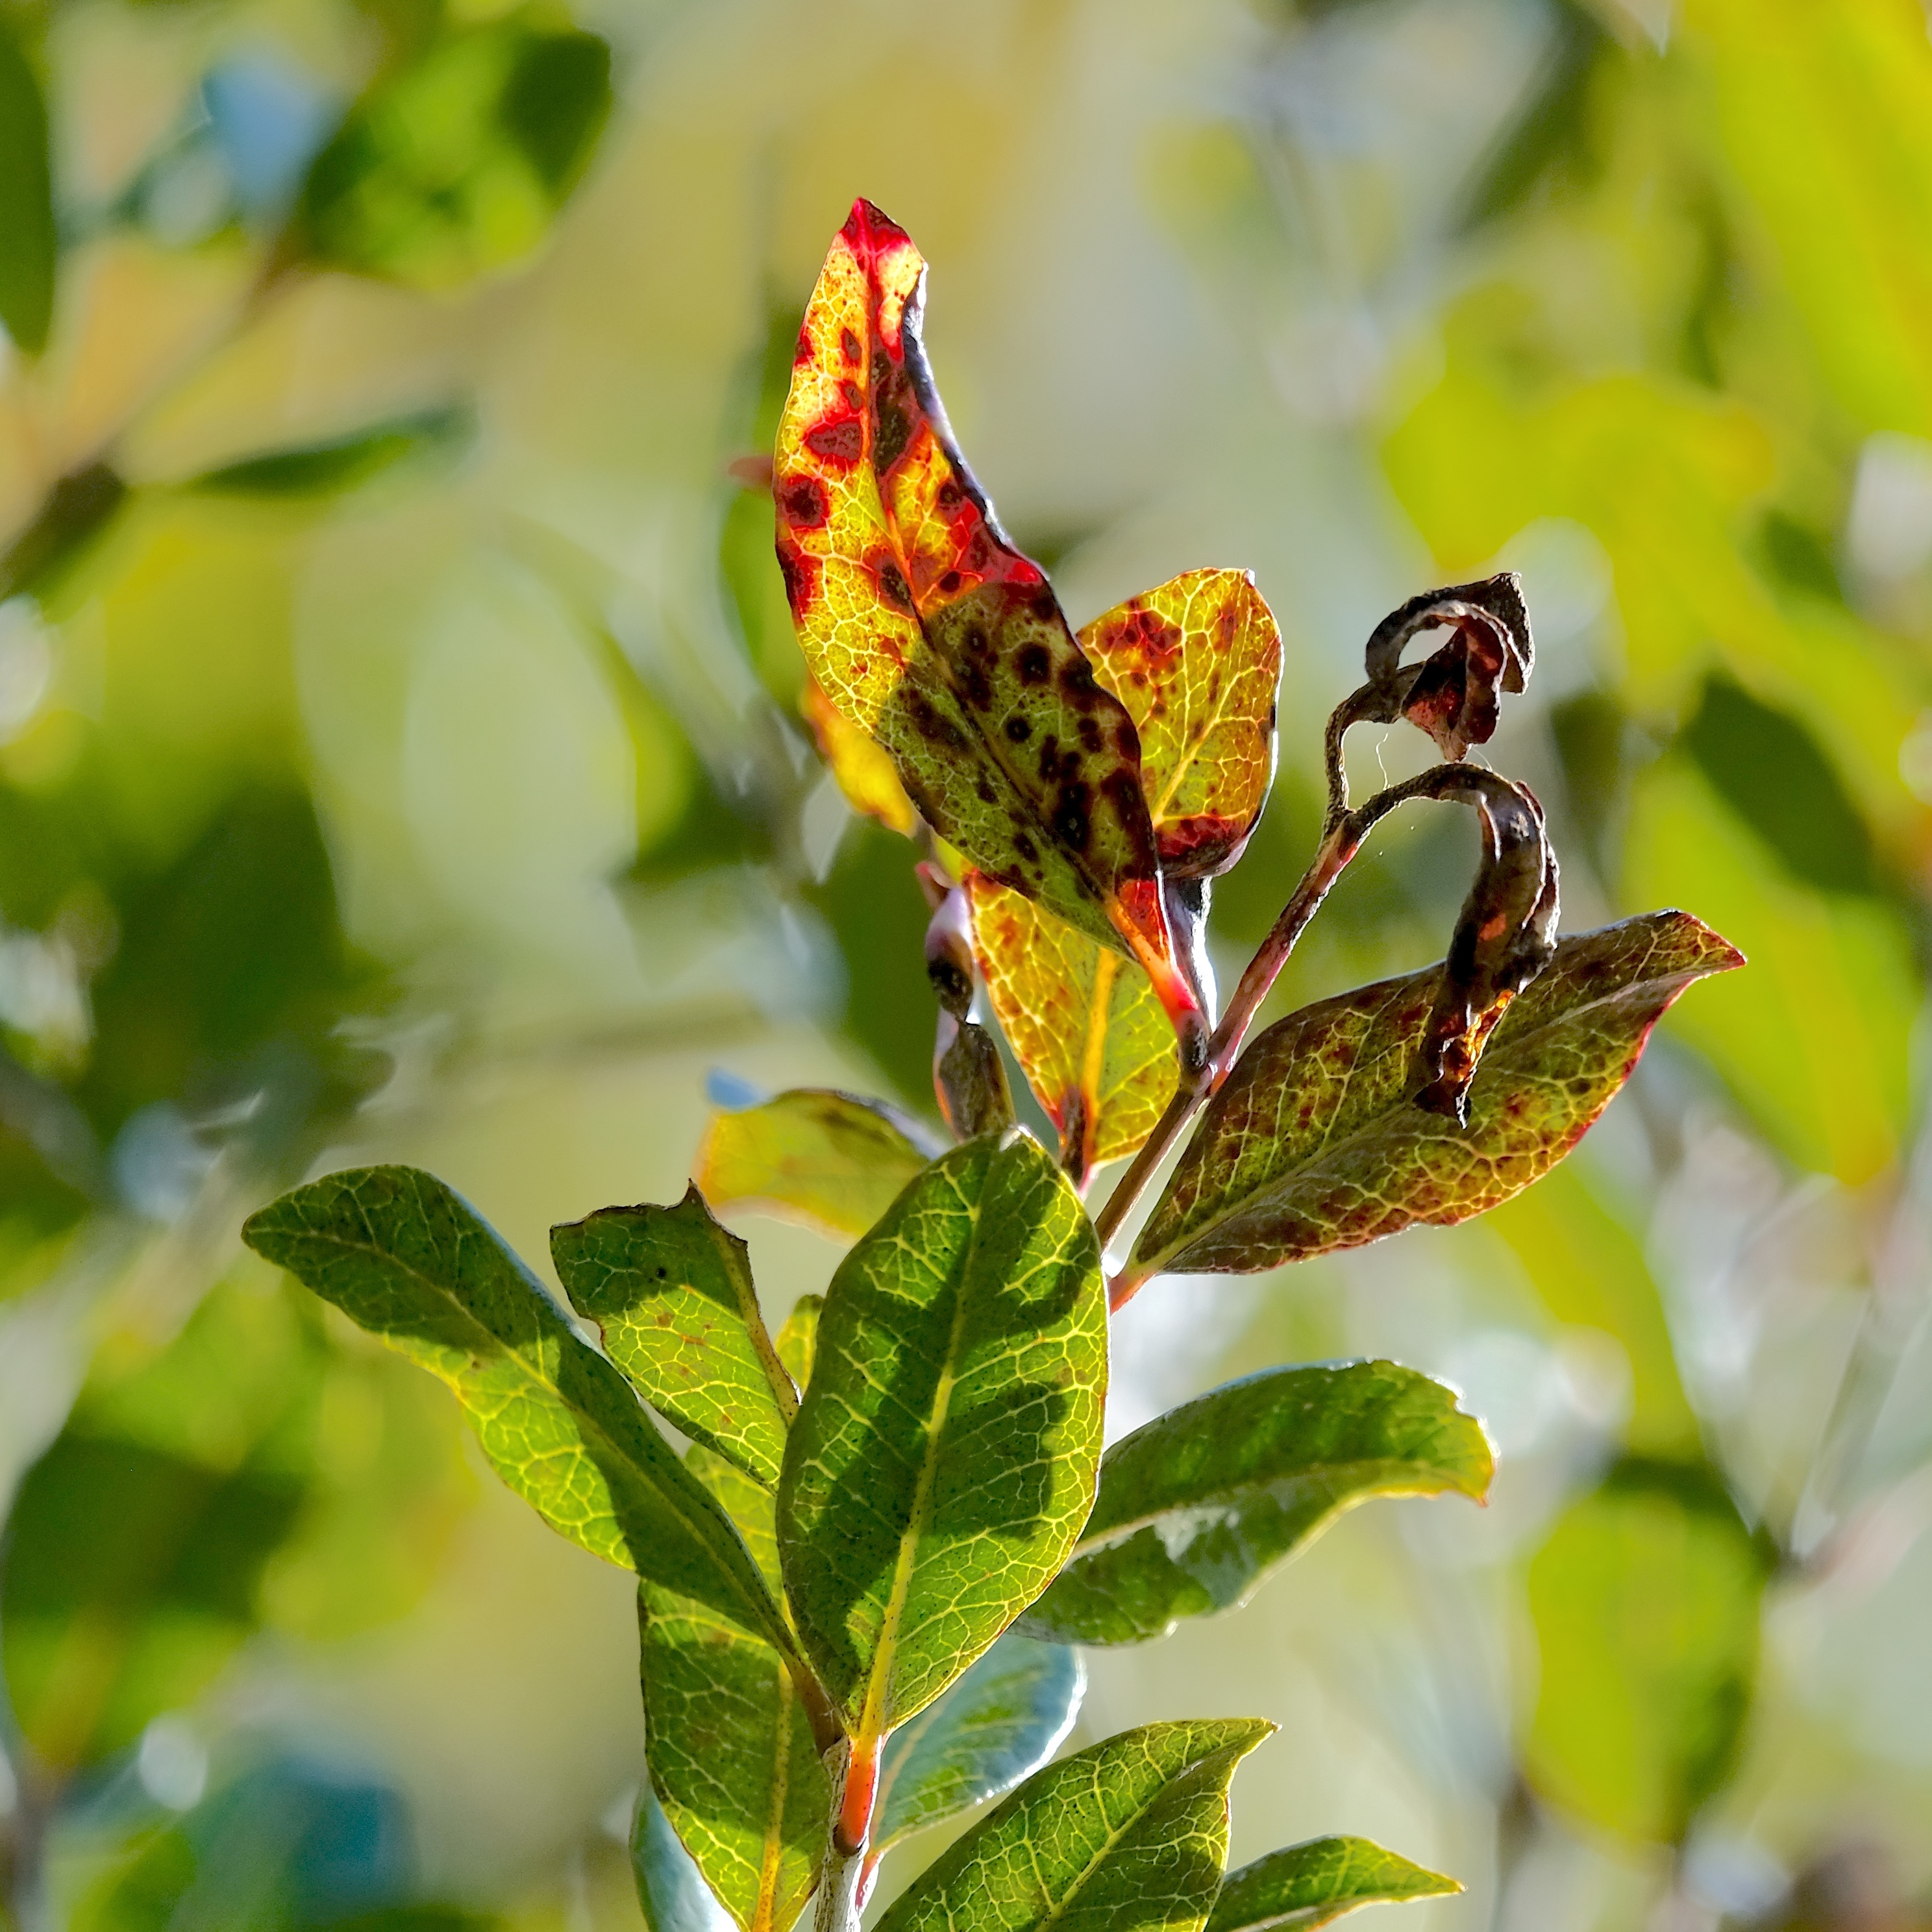
\includegraphics[keepaspectratio]{../2_1_figures/introduction/DSCF4043_cropped.JPG}}

}

\subcaption{\label{fig-red_blotches}Red blotches on leaves leading to
necrotic lesions and shoot tip dieback.}

\end{minipage}%

\end{figure}%

}

\caption[Myrtle rust symptoms on \emph{S.
maire}.]{\label{fig-symptoms}The \hyperref[acronyms_MR]{myrtle rust}
symptoms showing the advancement of \hyperref[acronyms_AP]{\emph{A.
psidii}} infection on \emph{S. maire}. Initial growth of yellow
urediniospores on leaves (\textbf{a}), and necrotic lesions and shoot
tip dieback (\textbf{b}).}

\end{figure}%

\section{Consequences of Myrtle Rust for New
Zealand}\label{consequences-of-myrtle-rust-for-new-zealand}

Since the pathogen's arrival in 2017 in New Zealand, at least 13 out of
30 native (\citeproc{ref-delangeConservationstatus2024}{De Lange et al.,
2024}) and 17 exotic Myrtaceae species are confirmed as hosts
(\citeproc{ref-toome-hellerChasingmyrtle2020}{Toome-Heller et al.,
2020}). Given the potential consequences of
\hyperref[acronyms_AP]{\emph{A. psidii}} infection,
\hyperref[acronyms_MR]{myrtle rust} poses far-reaching implications
across ecological, cultural and economic systems of Aotearoa. In woody
ecosystems successional plant communities and Myrtaceae-dominated
old-growth forests are at most risk
(\citeproc{ref-mccarthyFunctionalAssessment2024}{McCarthy et al.,
2024}). Widespread loss of Myrtaceae from \hyperref[acronyms_MR]{myrtle
rust} would cause substantial changes to the functional structure of New
Zealand's forests, particularly if multiple Myrtaceae species become
infected at the same site and co-occurring species lack the capacity to
compensate for their loss
(\citeproc{ref-mccarthyFunctionalAssessment2024}{McCarthy et al.,
2024}). Myrtaceae species are keystone species, and birds, reptiles,
bats and invertebrates feed on their nectar
(\citeproc{ref-gailbraithImplicationsselected2017}{Gailbraith \& Large,
2017}; \citeproc{ref-joEcologicalimportance2022}{Jo et al., 2022};
\citeproc{ref-sutherlandMonitoringAustropuccinia2020}{Sutherland et al.,
2020}). Furthermore, bats are reported to hunt for invertebrates above
Myrtaceae (\citeproc{ref-gailbraithImplicationsselected2017}{Gailbraith
\& Large, 2017}). However, while birds, bats and reptiles are projected
to be flexible enough to overcome decline of Myrtaceae, some
invertebrates are thought to have an obligate relationship with
Myrtaceae species
(\citeproc{ref-gailbraithImplicationsselected2017}{Gailbraith \& Large,
2017}). Beyond ecological concerns, many Myrtaceae are taonga (treasure)
species which hold profound cultural and spiritual significance for
Māori (\citeproc{ref-teulonthreatmyrtle2015}{Teulon et al., 2015}).
Furthermore, Myrtaceae species have significant economic value
(\citeproc{ref-essienValueaddedpotential2019}{Essien et al., 2019}).
Mānuka (\emph{Leptospermum scoparium}) honey generated NZ\$538 million
in 2022 and is projected to rise to over NZ\$1 billion by 2030
(\citeproc{ref-apiculturenewzealandNewZealand2024}{Apiculture New
Zealand, 2024}). Consequently, there is considerable concern about the
long-term impact of \hyperref[acronyms_MR]{myrtle rust} on the Myrtaceae
species, because of their importance to Māori culture, the New Zealand
economy, and its ecosystems.

\section{Management and Mitigation
Strategies}\label{management-and-mitigation-strategies}

\hyperref[acronyms_MR]{Myrtle rust} is considered to be established in
New Zealand since 2018, and efforts are focused on long-term mitigation
(\citeproc{ref-ministryforprimaryindustriesNewapproach2020}{Ministry for
Primary Industries, 2020}). Current strategies are targeted at
protecting susceptible species and reducing the rate of spread
(\citeproc{ref-beresfordGuidemyrtle2025}{Beresford, 2025}). These
include removal of infected plant parts, or entire plants with minimal
disturbance, and disposal in a manner that minimises the risk of further
spore dispersal. Where possible, pruning is recommended during cooler
seasons to avoid stimulating new growth. Additionally, clothing and
equipment should be disinfected between sites. Synthetic fungicides
offer an additional option for reducing infection severity and have
shown to be highly effective in treating \hyperref[acronyms_MR]{myrtle
rust} with low phytotoxicity
(\citeproc{ref-beresfordRiskbasedfungicide2022}{Beresford \& Wright,
2022}; \citeproc{ref-chngPotentialdisease2019}{Chng et al., 2019}).
However, their effectiveness depends on regular application, making them
costly and impractical for large-scale use
(\citeproc{ref-sutherlandMonitoringAustropuccinia2020}{Sutherland et
al., 2020}). Nevertheless, fungicide treatment may be viable in cases
where only a small number of trees require protection, provided that
their exact locations are known.

\section{\texorpdfstring{\emph{S. maire}: Ecology, Significance, and
Conservation
Challenges}{S. maire: Ecology, Significance, and Conservation Challenges}}\label{s.-maire-ecology-significance-and-conservation-challenges}

\subsection{Biology and Taxonomy}\label{biology-and-taxonomy}

\emph{Syzygium} is the most diverse tree genus globally, comprising over
1000 species (\citeproc{ref-lowGenomicinsights2022}{Low et al., 2022}),
and serves as an important food source for birds, mammals and insects
across the tropical Indo-Pacific
(\citeproc{ref-parnellj.a.n.MattersScale2007}{Parnell et al., 2007}).
Within New Zealand, \hyperref[acronyms_SM]{\emph{Syzygium maire}} is the
only native species of the Syzygium genus
(\citeproc{ref-delangeConservationstatus2024}{De Lange et al., 2024}).
\hyperref[acronyms_SM]{\emph{S. maire}} is a slender tree and can grow
up to 16 m tall with numerous branches and a compact crown, comprised of
\textasciitilde1.5 cm wide and \textasciitilde5cm long leaves
(Figure~\ref{fig-smaire}). It is characterised by specialised
pneumatophores (aerial roots), enabling it to inhabit waterlogged soils.
Between January and April, healthy and mature individuals produce white
brush flowers and bright red, one-seeded edible berries alongside
immature green fruit (\citeproc{ref-delangeConservationstatus2024}{De
Lange et al., 2024}; \citeproc{ref-Keikonei}{Mahuta et al., 2021};
\citeproc{ref-taranakiregionalcouncilBiodiversity}{Taranaki Regional
Council, n.d.}).

\begin{figure}

\centering{

\begin{figure}[H]

\begin{minipage}{0.49\linewidth}

\centering{

\pandocbounded{\includegraphics[keepaspectratio]{../2_1_figures/introduction/DJI_0845_cropped.JPG}}

}

\subcaption{\label{fig-smaire_stand}A stand of six \emph{S. maire} trees
with variable infection severity.}

\end{minipage}%
%
\begin{minipage}{0.02\linewidth}
~\end{minipage}%
%
\begin{minipage}{0.49\linewidth}

\centering{

\pandocbounded{\includegraphics[keepaspectratio]{../2_1_figures/introduction/DJI_20250801092659_0002_D_cropped.png}}

}

\subcaption{\label{fig-smaire_aerial}Aerial view of \emph{S. maire}
within mixed native forest canopy.}

\end{minipage}%

\end{figure}%

}

\caption[Examples of \emph{S. maire}.]{\label{fig-smaire}Examples of
\hyperref[acronyms_SM]{\emph{S. maire}} in urban parks of a separated
stand (\textbf{a}) and surrounded by vegetation (\textbf{b}). Arrows
indicate tree locations; colours represent dieback severity (white =
limited, light red = advanced, red = severe mortality).}

\end{figure}%

\subsection{Distribution, Habitat, and Conservation
Status}\label{distribution-habitat-and-conservation-status}

\hyperref[acronyms_SDM]{Species distribution models (SDMs)} indicate
that \hyperref[acronyms_SM]{\emph{S. maire}}'s historical habitat
spanned from the north of the South Island across most parts of the
North Island (\citeproc{ref-mccarthySpeciesdistribution2019}{McCarthy et
al., 2019}). \hyperref[acronyms_SM]{\emph{S. maire}} is most commonly
found in lowland wetlands with low water tables and along stream gullies
(\citeproc{ref-delangeConservationstatus2024}{De Lange et al., 2024};
\citeproc{ref-mccarthySpeciesdistribution2019}{McCarthy et al., 2019}).
Its pneumatophores enable it to be a dominant component of swamp
forests, where it often occurs alongside pukatea (\emph{Laurelia
novae-zelandiae}), a more widespread generalist species with similarly
small leaves (3 × 6 cm; Mahuta et al., 2021; Manaaki Whenua - Landcare
Research, 2025). Other co-occurring species include tawa
(\emph{Beilschmiedia tawa}), which also possess small leaves (1.4 × 6
cm), though narrower than those of \hyperref[acronyms_SM]{\emph{S.
maire}}
(\citeproc{ref-manaakiwhenua-landcareresearchNewZealand2026}{Manaaki
Whenua - Landcare Research, 2026}), and climbing plants such as kiekie
(\emph{Freycinetia banksii}), and supplejack (\emph{Ripogonum scandens};
Singers \& Rogers, 2014), which may establish within the canopy of
\hyperref[acronyms_SM]{\emph{S. maire}}. In addition, human-driven
deforestation and land drainage have restricted
\hyperref[acronyms_SM]{\emph{S. maire}} to a fraction of its original
distribution. It is estimated that only 10\% of New Zealand's wetlands
are still intact (\citeproc{ref-dymondRevisedextent2021}{Dymond et al.,
2021}). Consequently, \hyperref[acronyms_SM]{\emph{S. maire}} is in
decline and classified as ``Threatened--Nationally Vulnerable''
(\citeproc{ref-delangeConservationstatus2024}{De Lange et al., 2024}),
New Zealand's highest extinction risk category
(\citeproc{ref-andrewj.townsendNewZealand2008}{Townsend et al., 2008}).

\subsection{Ecological and Cultural
Significance}\label{ecological-and-cultural-significance}

Ecologically, \hyperref[acronyms_SM]{\emph{S. maire}} plays a critical
role in forest structure and function. Its fruits provide a food source
for native birds including kererū (\emph{Hemiphaga novaeseelandiae}),
tūī (\emph{Prosthemadera novaeseelandiae}), and korimako
(\emph{Anthornis melanura}; Van Der Walt et al., 2020), and its presence
provides structural habitat and shelter for some of New Zealand's most
threatened freshwater fish species (\citeproc{ref-Keikonei}{Mahuta et
al., 2021}). Notably, \hyperref[acronyms_SM]{\emph{S. maire}} can
achieve reproductive maturity early, with fruit production documented in
individuals five to ten years old
(\citeproc{ref-balkwillAdaptivePotential2025}{Balkwill et al., 2025}).
Like other Myrtaceae species, \hyperref[acronyms_SM]{\emph{S. maire}}
holds profound cultural and spiritual significance for Māori as taonga
species, valued as a source of kai (food), rongoā (medicine), dye,
perfume or air-freshener, and timber weapons for self-defence
(\citeproc{ref-balkwillDenovoassembly2024}{Balkwill et al., 2024};
\citeproc{ref-gouldAntioxidantactivities2006}{Gould et al., 2006};
\citeproc{ref-Keikonei}{Mahuta et al., 2021};
\citeproc{ref-taranakiregionalcouncilBiodiversity}{Taranaki Regional
Council, n.d.}). This cultural importance, combined with its ecological
role in swamp forests, ecosystems that have suffered widespread loss in
Aotearoa, underscores the conservation urgency for this species.

\subsection{Susceptibility to Myrtle Rust and Research
Gaps}\label{susceptibility-to-myrtle-rust-and-research-gaps}

\hyperref[acronyms_AP]{\emph{A. psidii}} infection severity varies
widely among host species
(\citeproc{ref-fernandezwinzerAustropucciniapsidii2019}{Fernandez Winzer
et al., 2019}). \hyperref[acronyms_SM]{\emph{S. maire}} is one of the
most susceptible Myrtaceae species to \hyperref[acronyms_AP]{\emph{A.
psidii}} infection (\citeproc{ref-beresfordGuidemyrtle2025}{Beresford,
2025}; \citeproc{ref-schmidShortCommunication2021}{Schmid et al.,
2021}), with mature trees capable of dying within three years of initial
infection (\citeproc{ref-delangeConservationstatus2024}{De Lange et al.,
2024}). Upon \hyperref[acronyms_AP]{\emph{A. psidii}}'s arrival in New
Zealand, the biology of \hyperref[acronyms_SM]{\emph{S. maire}} remained
scarcely researched and understood, contributing to the absence of a
robust conservation strategy. However, this research gap is being
progressively closed, with recent publications exploring genome assembly
(\citeproc{ref-balkwillDenovoassembly2024}{Balkwill et al., 2024}),
adaptive potential
(\citeproc{ref-balkwillAdaptivePotential2025}{Balkwill et al., 2025}),
and reproductive strategies
(\citeproc{ref-bettoniSexualasexual2024}{Bettoni et al., 2024}). Ex-situ
cryopreservation of \hyperref[acronyms_SM]{\emph{S. maire}} seeds is
also being investigated as a potential long-term conservation option,
though practical application remains unfeasible
(\citeproc{ref-nadarajanIntegratedex2021}{Nadarajan et al., 2021};
\citeproc{ref-vanderwaltSeeddevelopment2020}{Van Der Walt et al., 2020},
\citeproc{ref-vanderwaltImpactsRapid2022}{2022},
\citeproc{ref-vanderwaltAdvancescryopreservation2023}{2023};
\citeproc{ref-vanderwaltInvestigatingcryopreservation2021}{Van Der Walt,
2021}). Furthermore, \hyperref[acronyms_SM]{\emph{S. maire}} seeds
exhibit characteristics that prevent successful long-term freezing
(\citeproc{ref-vanderwaltAdvancescryopreservation2023}{Van Der Walt et
al., 2023}), limiting the viability of seed banking as a standalone
conservation strategy. These constraints place further emphasis on the
urgent need for in-situ conservation efforts, including improved mapping
and monitoring of remaining populations.

\section{\texorpdfstring{Current Mapping of
\hyperref[acronyms_SM]{\emph{S.
maire}}}{Current Mapping of S. maire}}\label{current-mapping-of}

Currently, \hyperref[acronyms_SM]{\emph{S. maire}} is predominantly
mapped using community science platforms like iNaturalist. While
iNaturalist is increasingly recognised as a valuable tool in
biodiversity research and used to develop species distribution models
(\citeproc{ref-masoniNaturalistaccelerates2025}{Mason et al., 2025}),
its data is inherently biased to areas with higher human activity and
accessibility. Geurts et al.
(\citeproc{ref-geurtsTurningobservations2023}{2023}) found that 94\% of
observations are within 1~km of roads, demonstrating the spatial bias of
such opportunistic datasets. Additionally, local conservation groups,
such as the
\href{https://kaipatiki.org.nz/our-work/eskdale-reserve/}{Kaipātiki
Project} or Friends of Bushglen Reserve, maintain records of
\hyperref[acronyms_SM]{\emph{S. maire}} locations within their
management areas. These known populations can provide the basis for
developing and validating automated detection methods. Beyond
discovering novel stands, \hyperref[acronyms_DL]{deep learning}-based
detection offers the advantage of automating repeated monitoring to
track tree health, growth, and infection progression over time. Another
approach consists of \hyperref[acronyms_SDM]{SDMs}, in which a
multifactorial \hyperref[acronyms_GIS]{GIS} analysis is developed to
identify their most probable habitat. Such a model already exists for
the greater Wellington region for \hyperref[acronyms_SM]{\emph{S.
maire}} (\citeproc{ref-herbertIdentifyingpotentially2025}{Herbert et
al., 2025}). However, such models only predict the likelihood of
occurrence, but not their exact location, which is critical for current
management approaches for \hyperref[acronyms_MR]{myrtle rust}.

\hyperref[acronyms_RS]{Remote sensing} has become a widely used tool for
tree species identification
(\citeproc{ref-changApplicationUAV2025}{Chang et al., 2025};
\citeproc{ref-zhongReviewTree2024}{L. Zhong et al., 2024}) and
represents a promising option to close the mapping gap for
\hyperref[acronyms_SM]{\emph{S. maire}}, which could be built on
\hyperref[acronyms_SDM]{SDM} outputs. However, applying these methods to
\hyperref[acronyms_SM]{\emph{S. maire}} presents inherent challenges:
the species' rarity makes gathering of reference data challenging, its
morphological overlap with co-occurring species, such as pukatea and
tawa, complicates identification, and the potential for climbing plants
to establish within its canopy further obscures individual trees for
detection on aerial imagery.

\section{Deep Learning for Species
Mapping}\label{deep-learning-for-species-mapping}

Tree detection in aerial imagery has followed the broader computer
vision trend toward \hyperref[acronyms_DL]{deep learning} solutions
(\citeproc{ref-lecunDeeplearning2015}{LeCun et al., 2015}). Even though
still used (\citeproc{ref-boschDetecTreeTree2020}{Bosch, 2020};
\citeproc{ref-malekEfficientFramework2014}{Malek et al., 2014};
\citeproc{ref-mirakiIndividualtree2021}{Miraki et al., 2021};
\citeproc{ref-safonovaIndividualTree2021}{Safonova et al., 2021}),
conventional \hyperref[acronyms_ML]{machine learning} methods, such as
\hyperref[acronyms_RF]{random forests (RFs)} or
\hyperref[acronyms_SVM]{support vector machines (SVMs)} that classify
individual pixels independently, have been outperformed by
\hyperref[acronyms_DL]{deep learning} methods
(\citeproc{ref-liuComparingfully2018}{Liu et al., 2018}), which can even
outperform humans in some cases
(\citeproc{ref-alzubaidiReviewdeep2021}{Alzubaidi et al., 2021}). Many
studies focus on tree segmentation as their primary objective: detecting
individual trees regardless of species
(\citeproc{ref-ballAccuratedelineation2023}{Ball et al., 2023};
\citeproc{ref-ganTreeCrown2023}{Gan et al., 2023};
\citeproc{ref-ulkuDeepSemantic2022}{Ulku et al., 2022}). Beyond this
foundational step, a more advanced and challenging task involves
species-level classification, where trees are identified and assigned to
their respective species
(\citeproc{ref-briechleClassificationTree2020}{Briechle et al., 2020};
\citeproc{ref-kattenbornConvolutionalNeural2019}{Kattenborn et al.,
2019}; \citeproc{ref-lobotorresApplyingFully2020}{Lobo Torres et al.,
2020}; \citeproc{ref-zhongIndividualTree2024}{H. Zhong et al., 2024}).
To achieve this species-level accuracy, there is a myriad of different
methodologies available, which broadly fall into two categories. These
are based on their underlying data type: architectures designed for
2D-sensed data, such as
\hyperref[acronyms_CNN]{convolutional neural networks (CNNs)} that learn
hierarchical spatial features from regular grid data
(e.g.~\hyperref[acronyms_UAV]{unmanned aerial vehicle (UAV)} or
satellite imagery), and architectures for 3D-sensed
\hyperref[acronyms_LiDAR]{light detection and ranging (LiDAR)} data that
operate on voxelised or point-cloud representations. Both are widely
used; however, because 2D approaches can draw on a broader range of data
sources (\hyperref[acronyms_RGB]{RGB} imagery,
\hyperref[acronyms_MS]{multispectral (MS)} imagery,
\hyperref[acronyms_HS]{hyperspectral (HS)} imagery) and are often more
cost-effective to acquire, there is substantially more
\hyperref[acronyms_DL]{deep learning} research in
\hyperref[acronyms_RS]{remote sensing} based on 2D-sensed than on
3D-sensed data (Figure~\ref{fig-bibliostats}; Zhong et al., 2024).

\begin{figure}

\centering{

\begin{figure}[H]

\begin{minipage}{0.10\linewidth}
~\end{minipage}%
%
\begin{minipage}{0.81\linewidth}

\pandocbounded{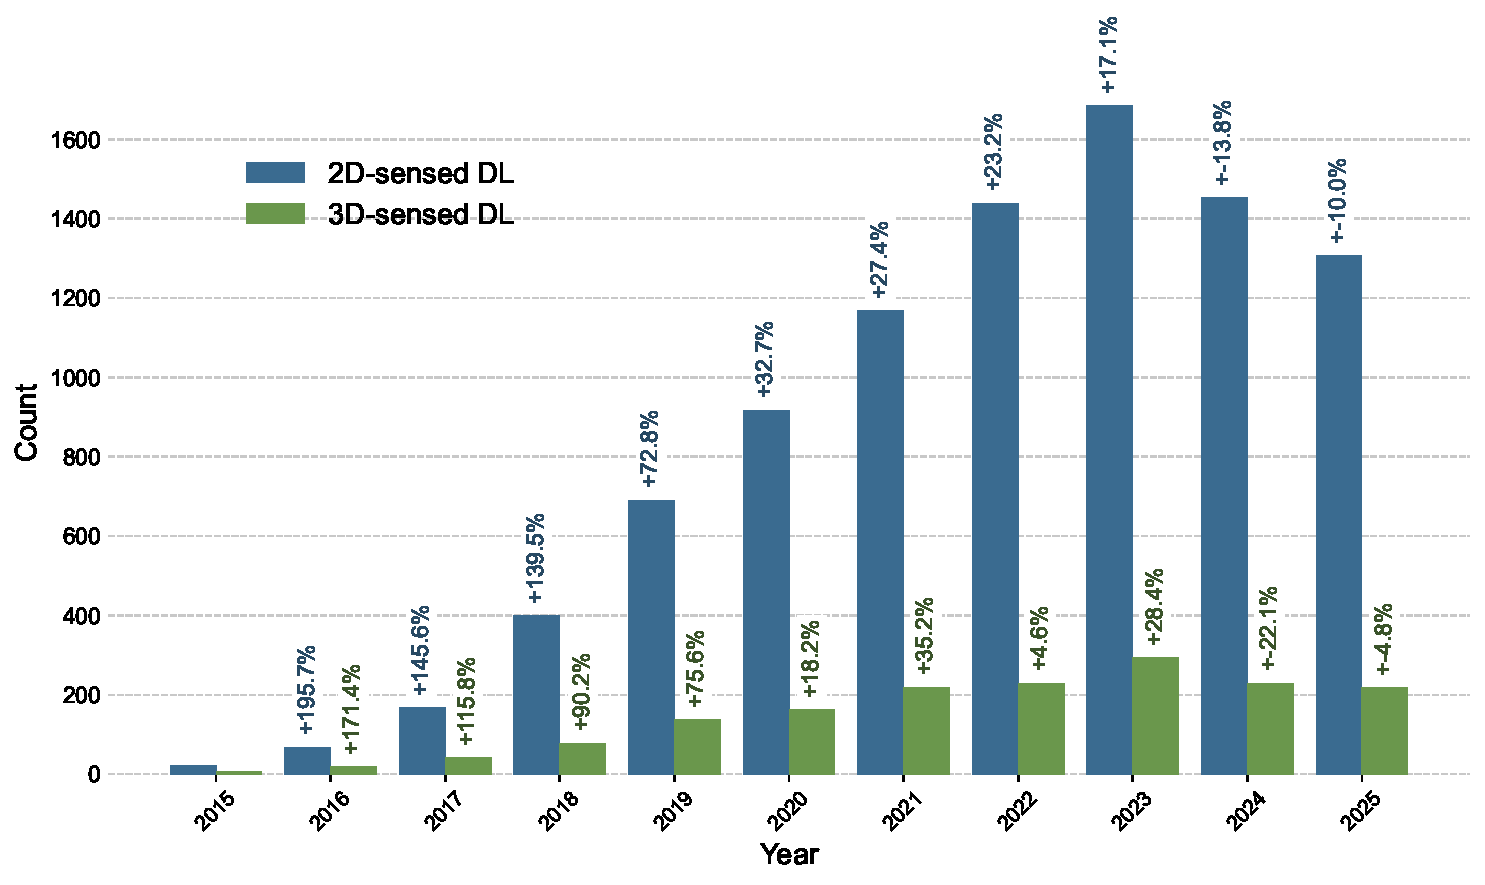
\includegraphics[keepaspectratio]{complete_thesis_files/figure-pdf/cell-2-output-1.pdf}}

\end{minipage}%
%
\begin{minipage}{0.10\linewidth}
~\end{minipage}%

\end{figure}%

}

\caption[Publications on grid- and point-based deep learning
articles.]{\label{fig-bibliostats}Total count and percentage increase
between successive years of peer-reviewed scientific articles in the
field of \hyperref[acronyms_RS]{remote sensing} related to
\hyperref[acronyms_DL]{deep learning} from 2015 - 2025. Blue represents
publications related to 2D-sensed and green to 3D-sensed data. Search
terms can be found in Appendix B and were retrieved from OpenAlex
(\citeproc{ref-priemOpenAlexfullyopen2022}{Priem et al., 2022}).}

\end{figure}%

\section{Deep Learning for Tree Species
Identification}\label{deep-learning-for-tree-species-identification}

\subsection{2D Semantic Segmentation}\label{d-semantic-segmentation}

\hyperref[acronyms_CNN]{CNNs} were originally designed for whole-image
classification tasks
(\citeproc{ref-krizhevskyImageNetclassification2017}{Krizhevsky et al.,
2017}) and have been applied by community science tools like
iNaturalist, Flora Incognita, and Pl@ntNet to identify plant species
from photographs (\citeproc{ref-dyrmannPlantspecies2016}{Dyrmann et al.,
2016}; \citeproc{ref-waldchenAutomatedplant2018}{Wäldchen et al.,
2018}). These networks revolutionised object detection through their
capacity to analyse image texture (contextual information from clusters
of neighbouring pixels) rather than evaluating pixels in isolation
(\citeproc{ref-cholletXceptionDeep2017}{Chollet, 2017}). They
autonomously learn which textural patterns (such as leaf morphology or
canopy characteristics) are relevant for distinguishing vegetation
communities and species (\citeproc{ref-dyrmannPlantspecies2016}{Dyrmann
et al., 2016}). In these architectures, sequential pooling operations
aggregate feature maps to progressively coarser spatial scales, with the
final layer indicating only whether distinct (species) features appear
anywhere within the image, without preserving their spatial locations.
This self-learning capacity provides substantial advantages in
computational efficiency and automation, eliminating manual feature
engineering required for traditional \hyperref[acronyms_ML]{machine
learning} (\citeproc{ref-maggioriHighResolutionAerial2017}{Maggiori et
al., 2017}). Combined with advances in high-resolution sensors,
\hyperref[acronyms_CNN]{CNNs} currently transform vegetation mapping
capabilities.

However, \hyperref[acronyms_RS]{remote sensing}-based vegetation mapping
demands more than whole-image classification can provide. For mapping
applications, success depends not on detecting whether the target class
exists, but on determining its precise spatial location throughout the
imagery, requiring spatially-continuous, detailed classification across
entire image extents
(\citeproc{ref-kattenbornConvolutionalNeural2019}{Kattenborn et al.,
2019}).
\hyperref[acronyms_FCNN]{Fully convolutional neural networks (FCNNs)}
address this limitation by retaining and reconstructing the spatial
locations of contextual features through encoder-decoder structures.
These networks extract contextual features whilst preserving spatial
origin, enabling fine-grained, spatial segmentation at the original
imagery resolution
(\citeproc{ref-maggioriHighResolutionAerial2017}{Maggiori et al., 2017};
\citeproc{ref-ronnebergerUNetConvolutional2015}{Ronneberger et al.,
2015}).

U-Net, originally developed for biomedical image segmentation
(\citeproc{ref-ronnebergerUNetConvolutional2015}{Ronneberger et al.,
2015}), has become a widely adopted \hyperref[acronyms_FCNN]{FCNN}
architecture for species detection in \hyperref[acronyms_RS]{remote
sensing} (\citeproc{ref-freudenbergLargeScale2019}{Freudenberg et al.,
2019}; \citeproc{ref-kattenbornConvolutionalNeural2019}{Kattenborn et
al., 2019}; \citeproc{ref-lakeDeeplearning2022}{Lake et al., 2022};
\citeproc{ref-ulkuDeepSemantic2022}{Ulku et al., 2022};
\citeproc{ref-wagnerUsingUnet2019}{Wagner et al., 2019};
\citeproc{ref-zhangIdentifyingmapping2020}{C. Zhang et al., 2020}). The
U-shaped encoder-decoder architecture progressively reduces spatial
resolution whilst increasing feature channels, enabling efficient
pixel-wise semantic classification. Although numerous
\hyperref[acronyms_FCNN]{FCNN} architectures exist, their performance
tends to be comparable to U-Net's
(\citeproc{ref-lobotorresApplyingFully2020}{Lobo Torres et al., 2020}).
In \hyperref[acronyms_MS]{MS} approaches, imagery is predominantly used
with traditional \hyperref[acronyms_ML]{machine learning} methods such
as \hyperref[acronyms_SVM]{SVMs}, yet is barely employed in
\hyperref[acronyms_CNN]{CNN}-based studies
(\citeproc{ref-zhongReviewTree2024}{L. Zhong et al., 2024}).

\subsection{3D Instance Segmentation and Point Cloud
Processing}\label{d-instance-segmentation-and-point-cloud-processing}

For 3D \hyperref[acronyms_LiDAR]{LiDAR} data, specialised neural network
architectures have been developed to process forest point clouds. These
methods leverage the vertical dimension and 3D tree crown geometry to
discriminate between species, offering complementary information to
spectral approaches (\citeproc{ref-henrichTreeLearndeep2024}{Henrich et
al., 2024}; \citeproc{ref-zhongIndividualTree2024}{H. Zhong et al.,
2024}). Two primary architectural approaches exist: voxel-based methods
that convert point clouds into regular 3D grids suitable for
convolutional operations
(\citeproc{ref-lecigneExploringtrees2018}{Lecigne et al., 2018};
\citeproc{ref-xiangAutomatedforest2024}{Xiang et al., 2024}), and
point-based architectures such as PointNet++ that process raw point
coordinates directly whilst preserving geometric detail
(\citeproc{ref-Qipointnet2017}{Qi et al., 2017}). Recent studies have
demonstrated successful species identification across diverse forest
types using these approaches
(\citeproc{ref-briechleClassificationTree2020}{Briechle et al., 2020}).

However, point cloud data presents unique preprocessing challenges
compared to imagery. Unlike raster data where spatial dimensions are
standardised through tile size, point clouds contain variable numbers of
points depending on forest structure and acquisition parameters. For
species-level classification, individual trees must first be isolated
(\citeproc{ref-briechleClassificationTree2020}{Briechle et al., 2020}).
This tree instance segmentation can be achieved through graph-based
methods such as Treeiso (\citeproc{ref-xi3DGraphBased2022}{Xi \&
Hopkinson, 2022}) or deep learning approaches like TreeLearn
(\citeproc{ref-henrichTreeLearndeep2024}{Henrich et al., 2024}). Once
individual trees are extracted, point counts must be normalised to
provide consistent neural network inputs, either through voxelisation
into fixed grid sizes or through resampling to a standard number of
points per tree. These preprocessing requirements add complexity but
enable the exploitation of 3D structural information to potentially use
for species identification.

\section{Scope and Novelty}\label{scope-and-novelty}

A critical challenge to detect rare species is severe class imbalance
combined with limited training data. Most published studies report
target classes comprising 30--50\% of annotated pixels
(\citeproc{ref-lobotorresApplyingFully2020}{Lobo Torres et al., 2020}),
whereas rare species in complex, biodiverse forests present
significantly different characteristics. These challenges create a
substantial gap between studies on readily detectable species
(\citeproc{ref-pearseDeepLearning2021}{Pearse et al., 2021}) and
operational requirements for rare species in complex ecosystems.
\hyperref[acronyms_SM]{\emph{S. maire}} shares morphological
similarities with co-occurring native species, possesses small leaves
that are difficult to resolve at typical \hyperref[acronyms_UAV]{UAV}
flight altitudes, and is a rare and conservation-critical New Zealand
tree species highly vulnerable to \hyperref[acronyms_MR]{myrtle rust}.
These characteristics, combined with its active management in local
parks and forests, make it an ideal species for a case study to evaluate
whether current deep learning approaches can successfully map rare,
morphologically inconspicuous species in complex forest environments.

Therefore, this thesis addresses four research questions: (1) Can
current \hyperref[acronyms_DL]{deep learning} approaches successfully
detect and delineate \hyperref[acronyms_SM]{\emph{S. maire}} in complex,
dense native forest despite severe class imbalance, morphological
similarity to co-occurring species, and limited training data? (2) How
do spectral characteristics (\hyperref[acronyms_RGB]{RGB} imagery
vs.~\hyperref[acronyms_MS]{MS} imagery) and hyperparameter
configurations affect detection performance? (3) Can models that are
trained on multiple sites generalise across all locations and outperform
models trained on a single site? (4) Can readily available 3D
LiDAR-based point-cloud segmentation algorithms supplement 2D-based
\hyperref[acronyms_FCNN]{FCNN} detection?

To address these questions, two complementary methodologies were
evaluated to test whether structural and spectral information could
improve detection under the given constraints: (1) a 2D
\hyperref[acronyms_FCNN]{FCNN} semantic segmentation approach using
\hyperref[acronyms_RGB]{RGB} imagery and \hyperref[acronyms_MS]{MS}
imagery data, which exploits spectral and spatial texture information at
high resolution, and (2) a 3D point cloud-based approach using
\hyperref[acronyms_LiDAR]{LiDAR} data with tree instance segmentation
(Figure~\ref{fig-wf_overall}). We hypothesise that structural
information (3D crown geometry, vertical position relative to other
trees) and spectral information (foliage reflectance, vegetation
indices) may provide complementary signals for species discrimination,
particularly for small-leaved species where morphological
distinctiveness is subtle. While the deep learning portion of this
thesis ultimately focusses on the first method, the evaluation aimed to
assess how both these methods could benefit species discrimination.
Furthermore, evaluating both methods provides insights into whether
complex forest environments require multi-modal data fusion or whether
single modalities suffice under current sensor and algorithmic
constraints.

\begin{figure}

\centering{

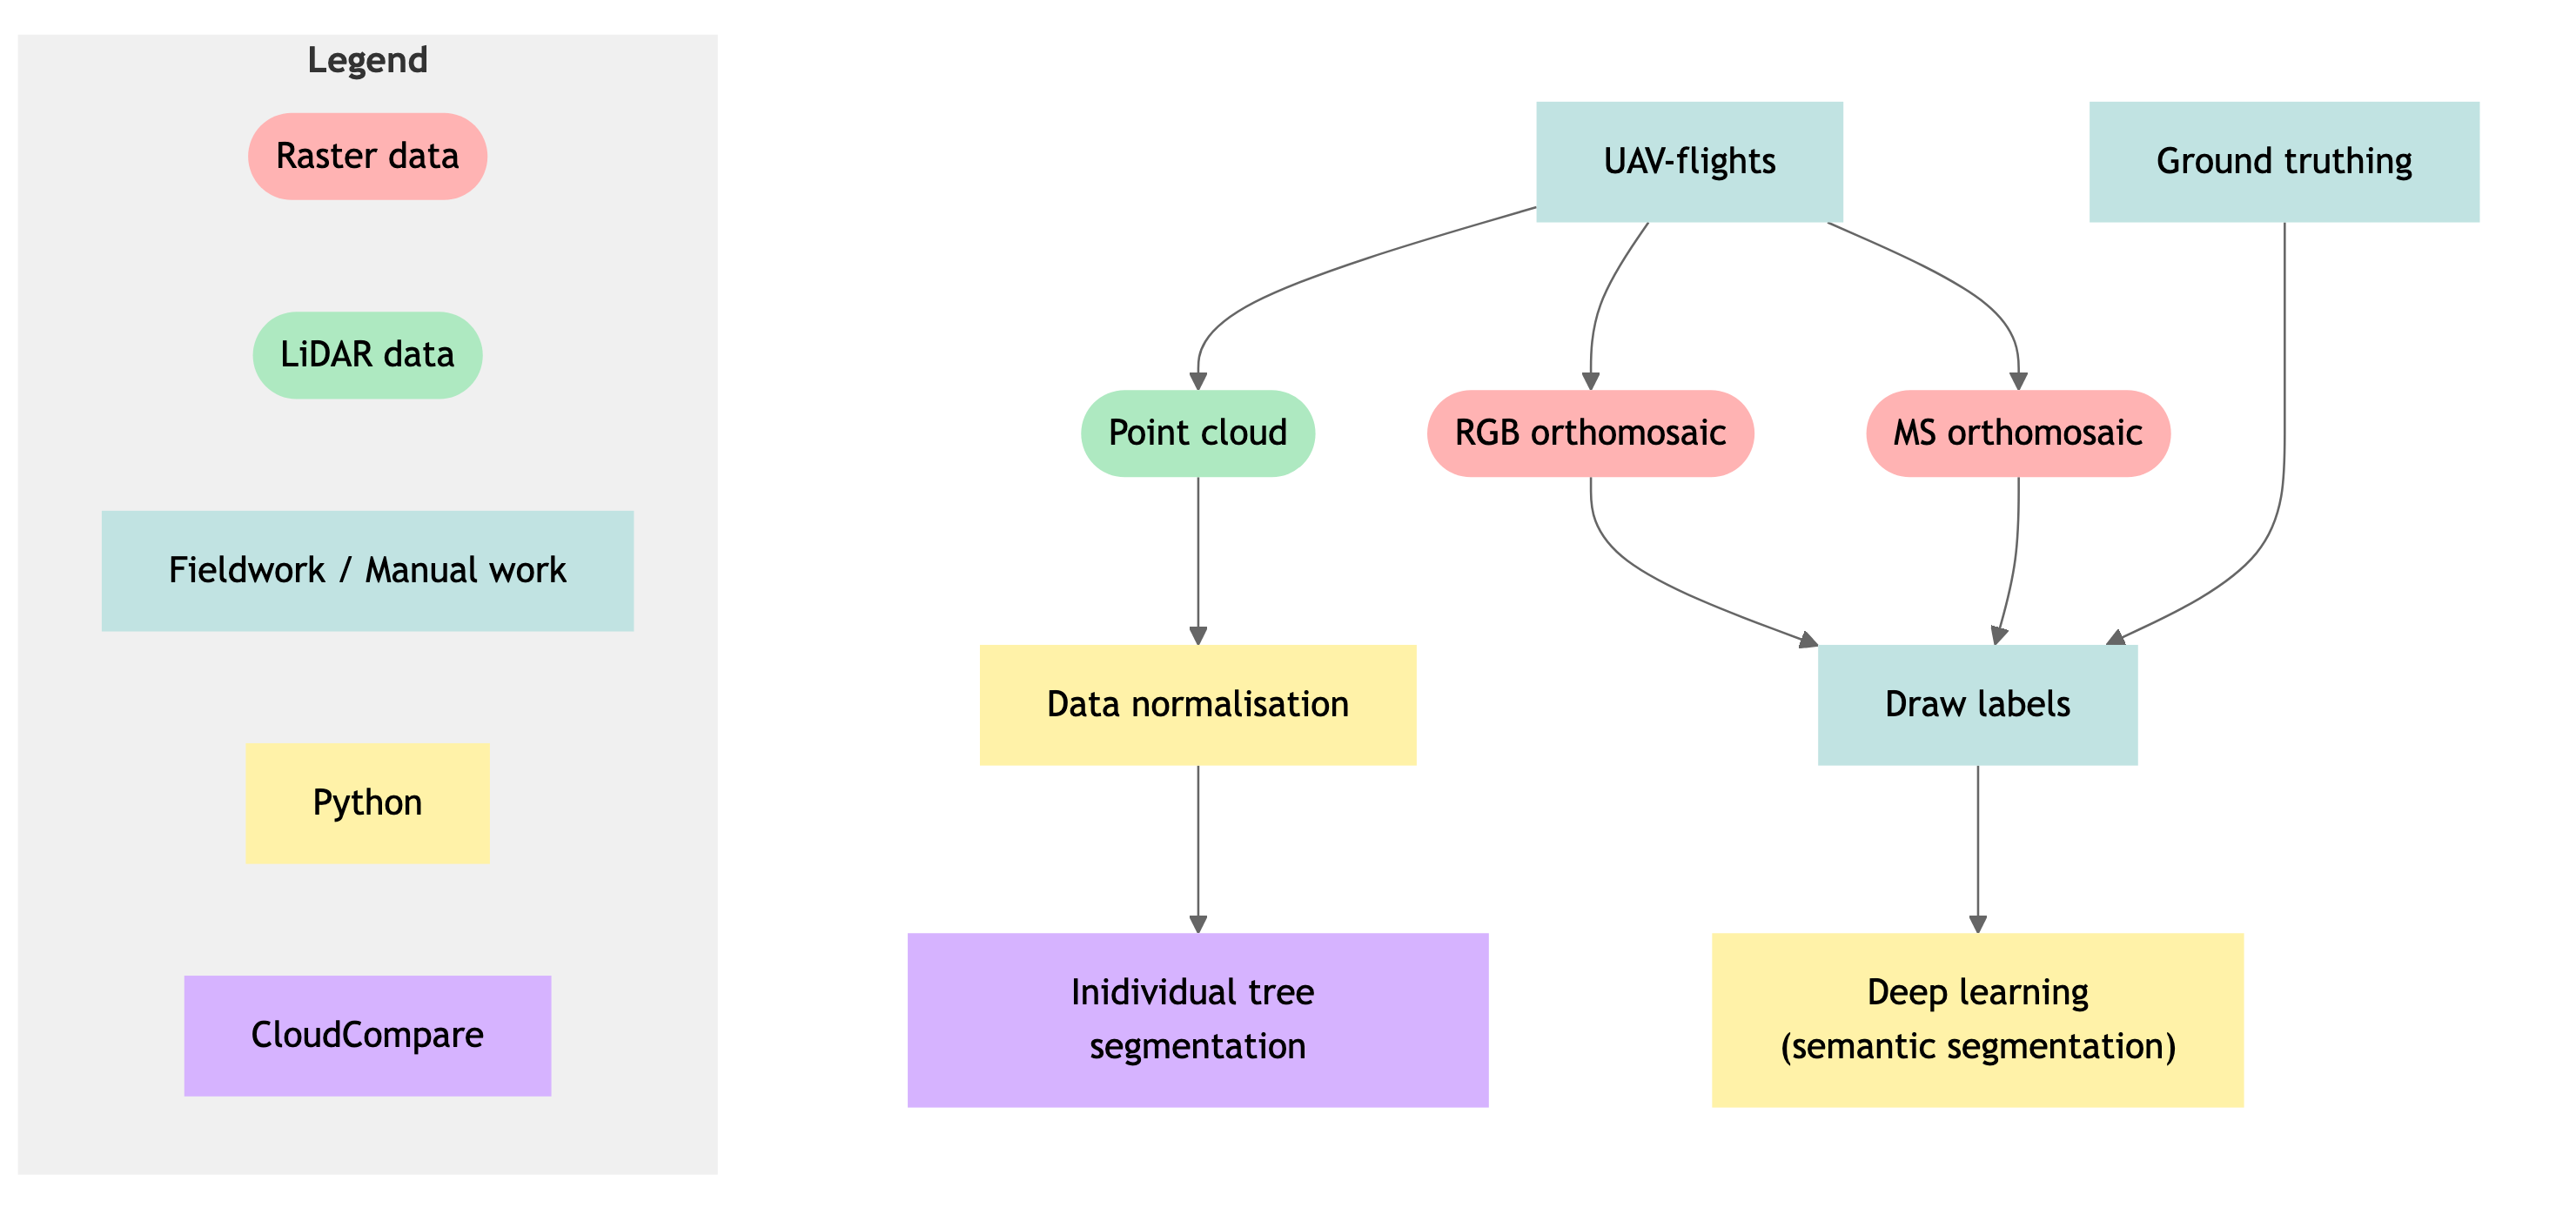
\includegraphics[width=6.5in,height=3.05in]{complete_thesis_files/figure-latex/mermaid-figure-1.png}

}

\caption[Overview methodology workflow.]{\label{fig-wf_overall}The
approach this thesis took for the identification of \emph{S. maire} on
UAV-collected data. The main focus is on the 2D-based deep learning
approach, but the capabilities of 3D-based segmentation are also
qualitatively evaluated.}

\end{figure}%

The research scope encompasses four urban forest reserves in the North
Island of New Zealand with known \hyperref[acronyms_SM]{\emph{S. maire}}
populations. By explicitly testing on a rare species in dense,
biodiverse forests rather than on readily detectable canopy dominants,
this thesis explores operational capabilities and limitations of current
\hyperref[acronyms_UAV]{UAV}-\hyperref[acronyms_DL]{deep learning}
approaches for conservation applications.

\chapter{Chapter 2 Methodology}\label{methodology}

\section{Research Sites}\label{sec-research_sites}

The thesis was conducted in four urban parks in Auckland and Hamilton,
New Zealand (Figure~\ref{fig-overview}). Site selection was guided by
known occurrences of \hyperref[acronyms_SM]{\emph{S. maire}} as reported
on \href{https://inaturalist.nz/taxa/406378-Syzygium-maire}{iNaturalist}
and by local conservation groups. Additional sites were scouted around
Tauranga, Auckland and Hamilton but were not considered further due to
limited presence (\textless{} five individuals) or complete or highly
advanced mortality of \hyperref[acronyms_SM]{\emph{S. maire}}. The final
four sites were selected based on a minimum of five trees and an age
range of approximately 20--60 years, ensuring cross-site comparability.

\begin{figure}[H]

\centering{

\pandocbounded{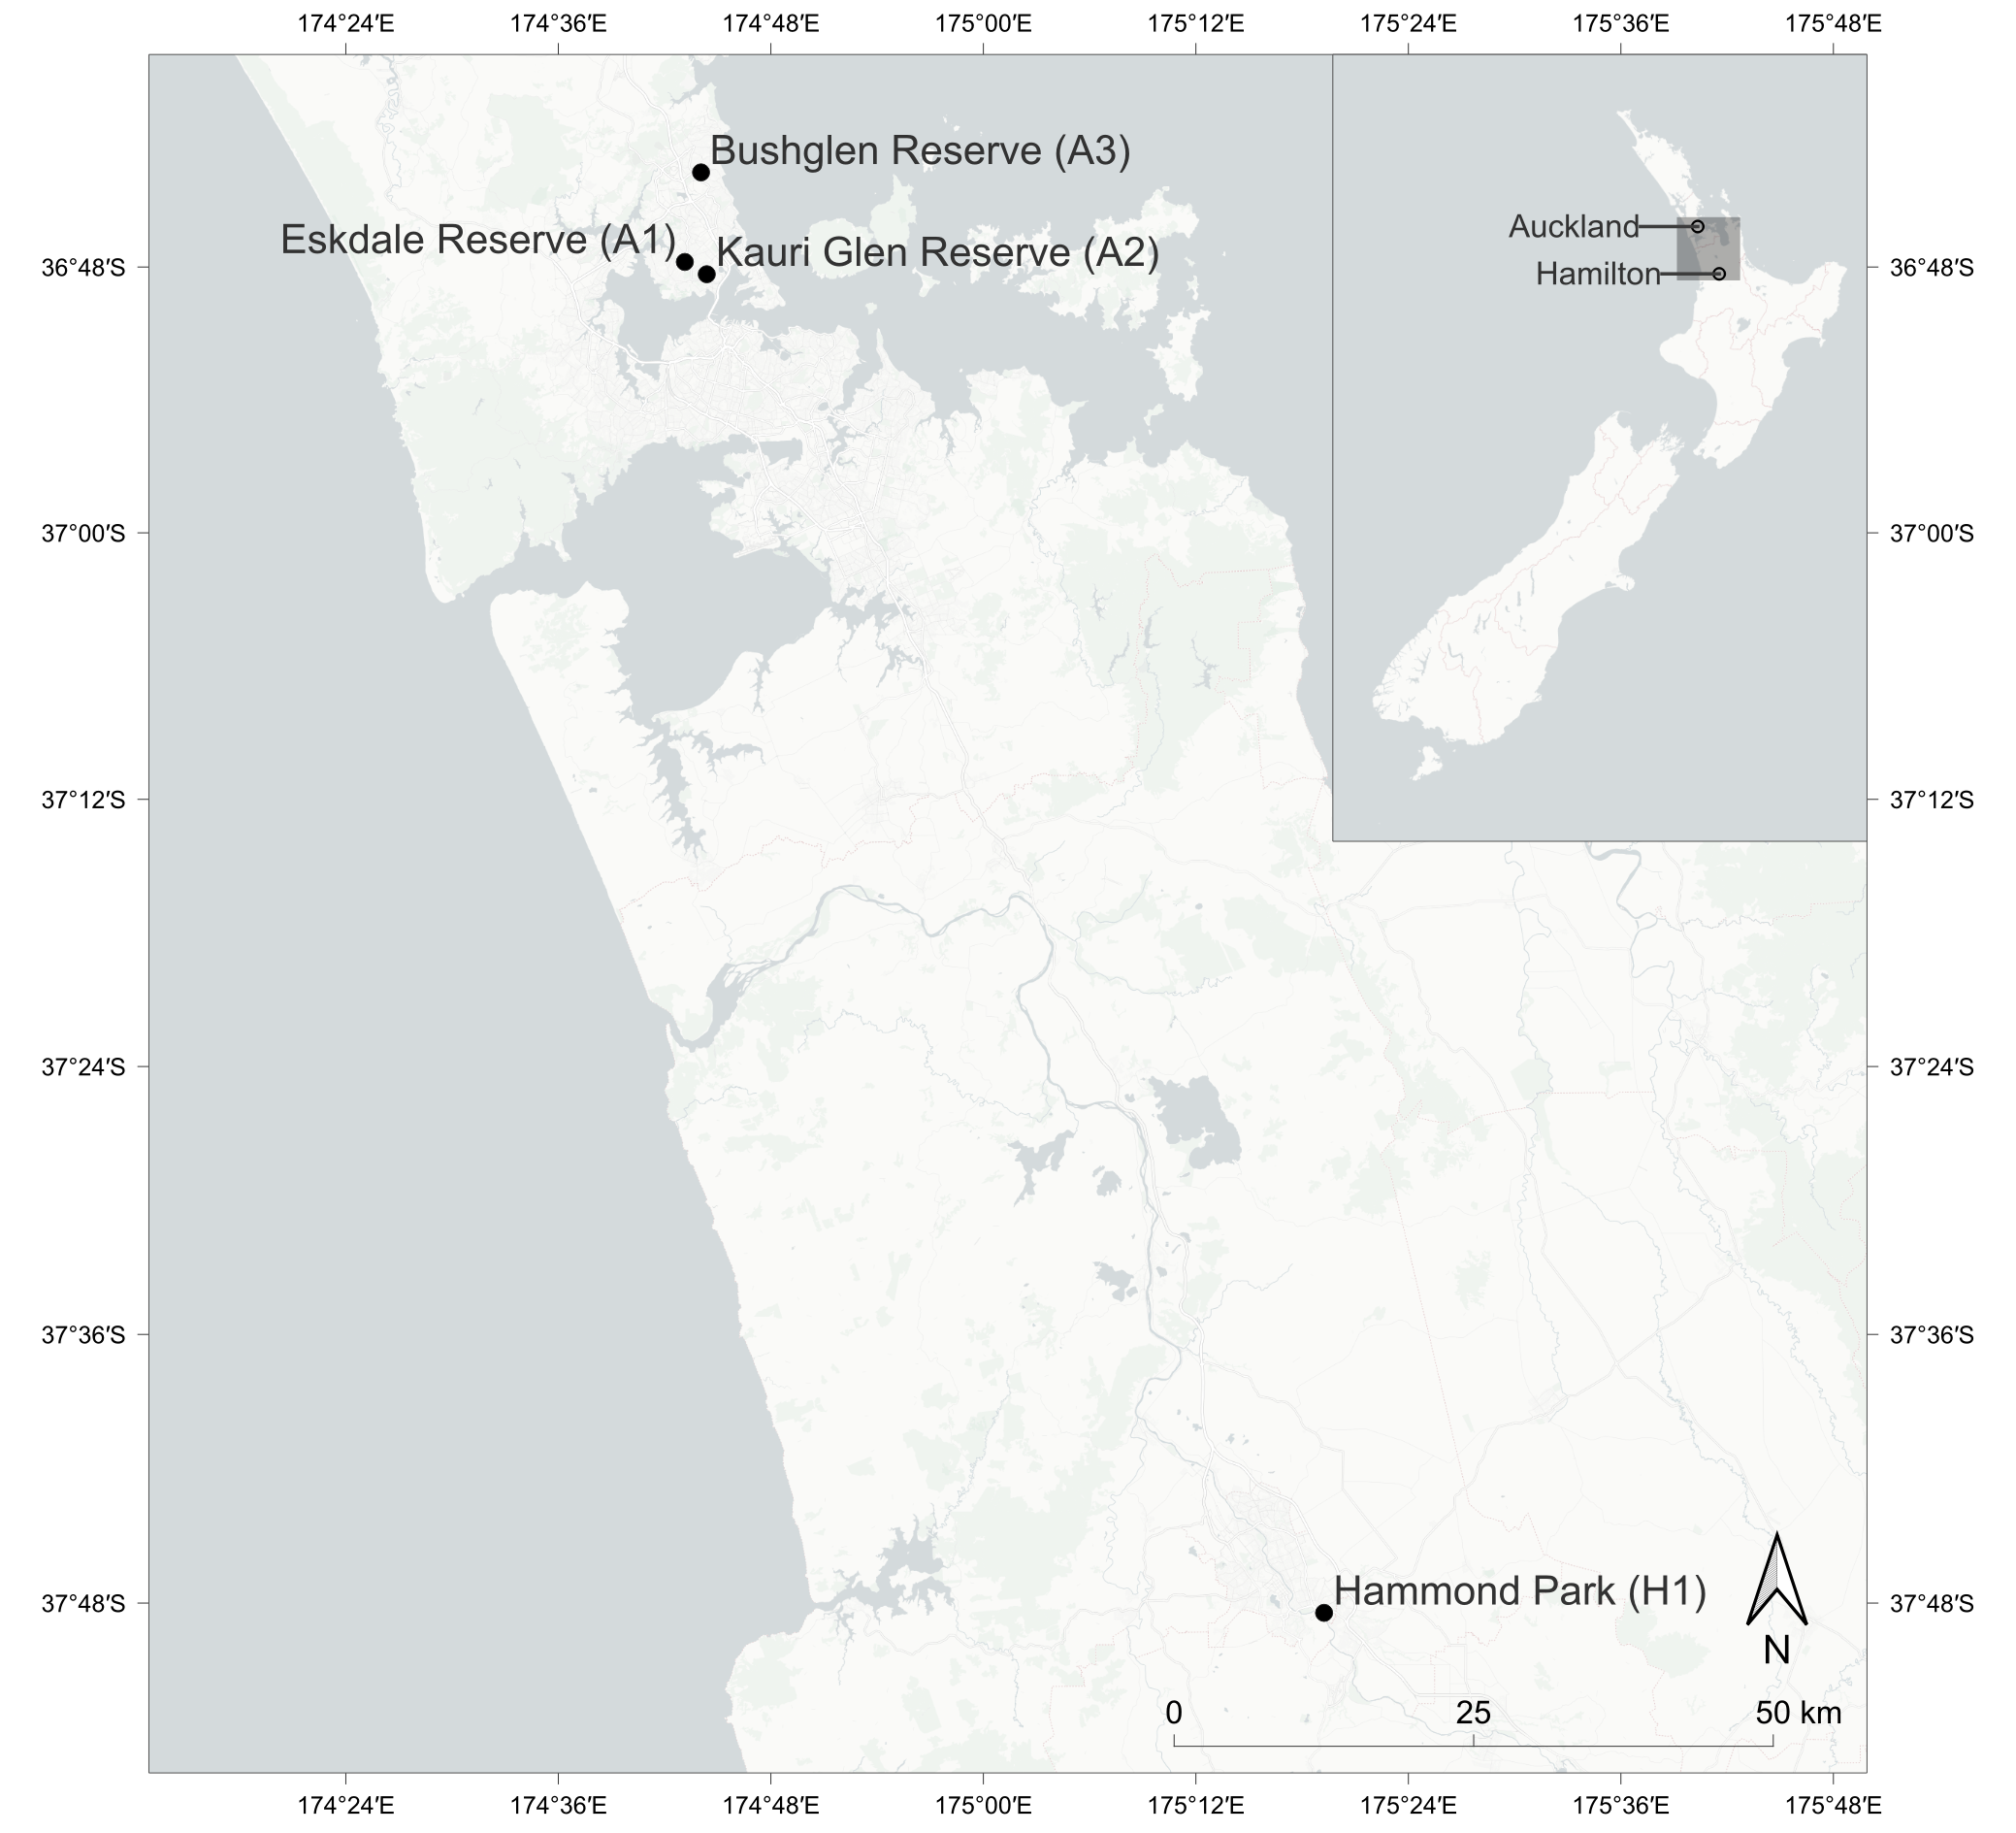
\includegraphics[keepaspectratio]{../2_1_figures/overview.png}}

}

\caption[Overview of research sites.]{\label{fig-overview}Overview of
the four research sites, of which all are located within urban parks.
Three are located in Auckland and one in Hamilton. Basemap: Copyright
CARTO and \href{https://www.openstreetmap.org}{OpenStreetMap}
contributors under
\href{https://opendatacommons.org/licenses/odbl/}{ODbl} by
\href{https://osmfoundation.org/}{OSFM}.}

\end{figure}%

The regrowth forest at all sites is classified as
\hyperref[acronyms_WF8]{warm temperate forest type 8 (WF8)}: Kahikatea,
pukatea forest (\citeproc{ref-singersclassificationNew2014}{Singers \&
Rogers, 2014}). This forest type comprises a podocarp and broadleaved
community dominated by kahikatea (\emph{Dacrycarpus dacrydioides}) with
scattered pukatea, kiekie and supplejack, and occasional rimu
(\emph{Dacrydium cupressinum}), tawa and \hyperref[acronyms_SM]{\emph{S.
maire}}, predominantly on organic and gley soils characterised by
elevated water tables. The canopy consists of a dense, complex matrix of
tree species, making visual identification of
\hyperref[acronyms_SM]{\emph{S. maire}} challenging, especially given
the similar appearance of co-occurring native trees. The sites are
surrounded by residential housing, ranging from 2.5--40 ha
(Table~\ref{tbl-overview}), though \hyperref[acronyms_SM]{\emph{S.
maire}} was only present in small portions of each site
(Figure~\ref{fig-sites_extent}). On three sites (A1--A3),
\hyperref[acronyms_SM]{\emph{S. maire}} is under fungicide spray
management, whilst H1 is unmanaged (Table~\ref{tbl-overview}; R.
Beresford, personal communication, October 29, 2025).

\begin{longtable}[]{@{}
  >{\raggedright\arraybackslash}p{(\linewidth - 14\tabcolsep) * \real{0.2333}}
  >{\raggedright\arraybackslash}p{(\linewidth - 14\tabcolsep) * \real{0.0778}}
  >{\raggedright\arraybackslash}p{(\linewidth - 14\tabcolsep) * \real{0.0778}}
  >{\raggedright\arraybackslash}p{(\linewidth - 14\tabcolsep) * \real{0.1333}}
  >{\raggedright\arraybackslash}p{(\linewidth - 14\tabcolsep) * \real{0.2889}}
  >{\raggedright\arraybackslash}p{(\linewidth - 14\tabcolsep) * \real{0.0444}}
  >{\raggedright\arraybackslash}p{(\linewidth - 14\tabcolsep) * \real{0.0778}}
  >{\raggedright\arraybackslash}p{(\linewidth - 14\tabcolsep) * \real{0.0667}}@{}}
\caption{Summary of the research sites with
\hyperref[acronyms_SM]{\emph{S. maire}} populations.
\hyperref[acronyms_LiDAR]{LiDAR} captures at Eskdale Reserve (A1)
consisted of one nadir and four oblique flight legs, while those at
Kauri Glen (A2) consisted of one nadir and two oblique flight legs.
Number refers to the number of \hyperref[acronyms_SM]{\emph{S. maire}}
canopies visible on aerial imagery. Area is for the entire forest within
that park. Train refers to the area of the training zone and te st to
the area of the test zone
(Figure~\ref{fig-sites_extent}).}\label{tbl-overview}\tabularnewline
\toprule\noalign{}
\begin{minipage}[b]{\linewidth}\raggedright
Name
\end{minipage} & \begin{minipage}[b]{\linewidth}\raggedright
Code
\end{minipage} & \begin{minipage}[b]{\linewidth}\raggedright
Num.
\end{minipage} & \begin{minipage}[b]{\linewidth}\raggedright
Fungicide
\end{minipage} & \begin{minipage}[b]{\linewidth}\raggedright
UAV-data
\end{minipage} & \begin{minipage}[b]{\linewidth}\raggedright
Area (ha)
\end{minipage} & \begin{minipage}[b]{\linewidth}\raggedright
Train (m\textsuperscript{2})
\end{minipage} & \begin{minipage}[b]{\linewidth}\raggedright
Test (m\textsuperscript{2})
\end{minipage} \\
\midrule\noalign{}
\endfirsthead
\toprule\noalign{}
\begin{minipage}[b]{\linewidth}\raggedright
Name
\end{minipage} & \begin{minipage}[b]{\linewidth}\raggedright
Code
\end{minipage} & \begin{minipage}[b]{\linewidth}\raggedright
Num.
\end{minipage} & \begin{minipage}[b]{\linewidth}\raggedright
Fungicide
\end{minipage} & \begin{minipage}[b]{\linewidth}\raggedright
UAV-data
\end{minipage} & \begin{minipage}[b]{\linewidth}\raggedright
Area (ha)
\end{minipage} & \begin{minipage}[b]{\linewidth}\raggedright
Train (m\textsuperscript{2})
\end{minipage} & \begin{minipage}[b]{\linewidth}\raggedright
Test (m\textsuperscript{2})
\end{minipage} \\
\midrule\noalign{}
\endhead
\bottomrule\noalign{}
\endlastfoot
Eskdale Reserve & A1 & 15 & 2023 &
\hyperref[acronyms_RGB]{RGB}/\hyperref[acronyms_MS]{MS},
\hyperref[acronyms_LiDAR]{LiDAR} (1+4) & 40 & 2,916 & 426 \\
Kauri Glen Res. & A2 & 17 & 2023 &
\hyperref[acronyms_RGB]{RGB}/\hyperref[acronyms_MS]{MS},
\hyperref[acronyms_LiDAR]{LiDAR} (1+2) & 21 & 1,667 & 306 \\
Bushglen Res. & A3 & 23 & 2022 &
\hyperref[acronyms_RGB]{RGB}/\hyperref[acronyms_MS]{MS} & 2.5 & 3,017 &
405 \\
Hammond Park & H1 & 15 & No &
\hyperref[acronyms_RGB]{RGB}/\hyperref[acronyms_MS]{MS} & 6 & 1,428 &
324 \\
\end{longtable}

\begin{figure}

\centering{

\begin{figure}[H]

\begin{minipage}{0.50\linewidth}

\centering{

\pandocbounded{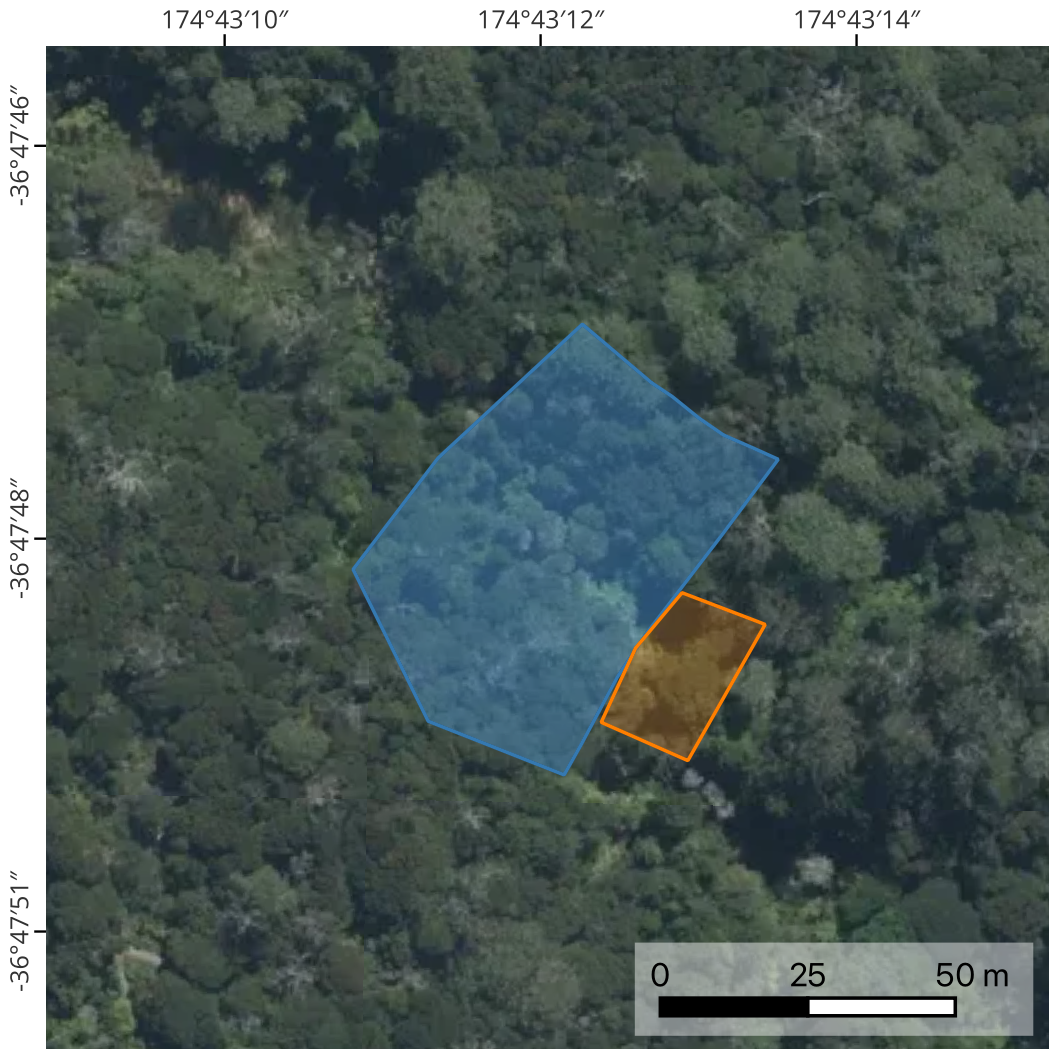
\includegraphics[keepaspectratio]{../2_1_figures/method/A1_sites_overview.png}}

}

\subcaption{\label{fig-sites_extent_A1}Eskdale Reserve (A1)}

\end{minipage}%
%
\begin{minipage}{0.50\linewidth}

\centering{

\pandocbounded{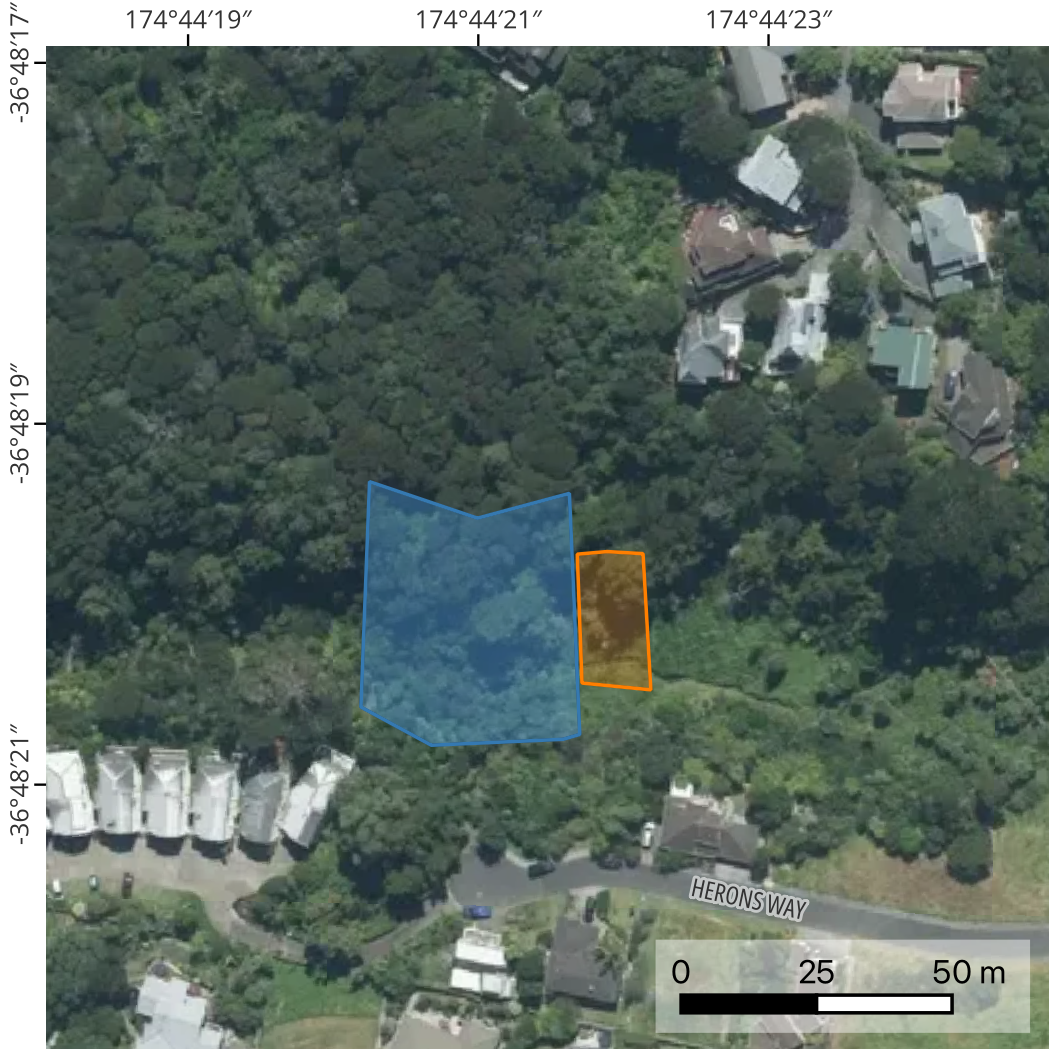
\includegraphics[keepaspectratio]{../2_1_figures/method/A2_sites_overview.png}}

}

\subcaption{\label{fig-sites_extent_A2}Kauri Glen Reserve (A2)}

\end{minipage}%
\newline
\begin{minipage}{0.50\linewidth}

\centering{

\pandocbounded{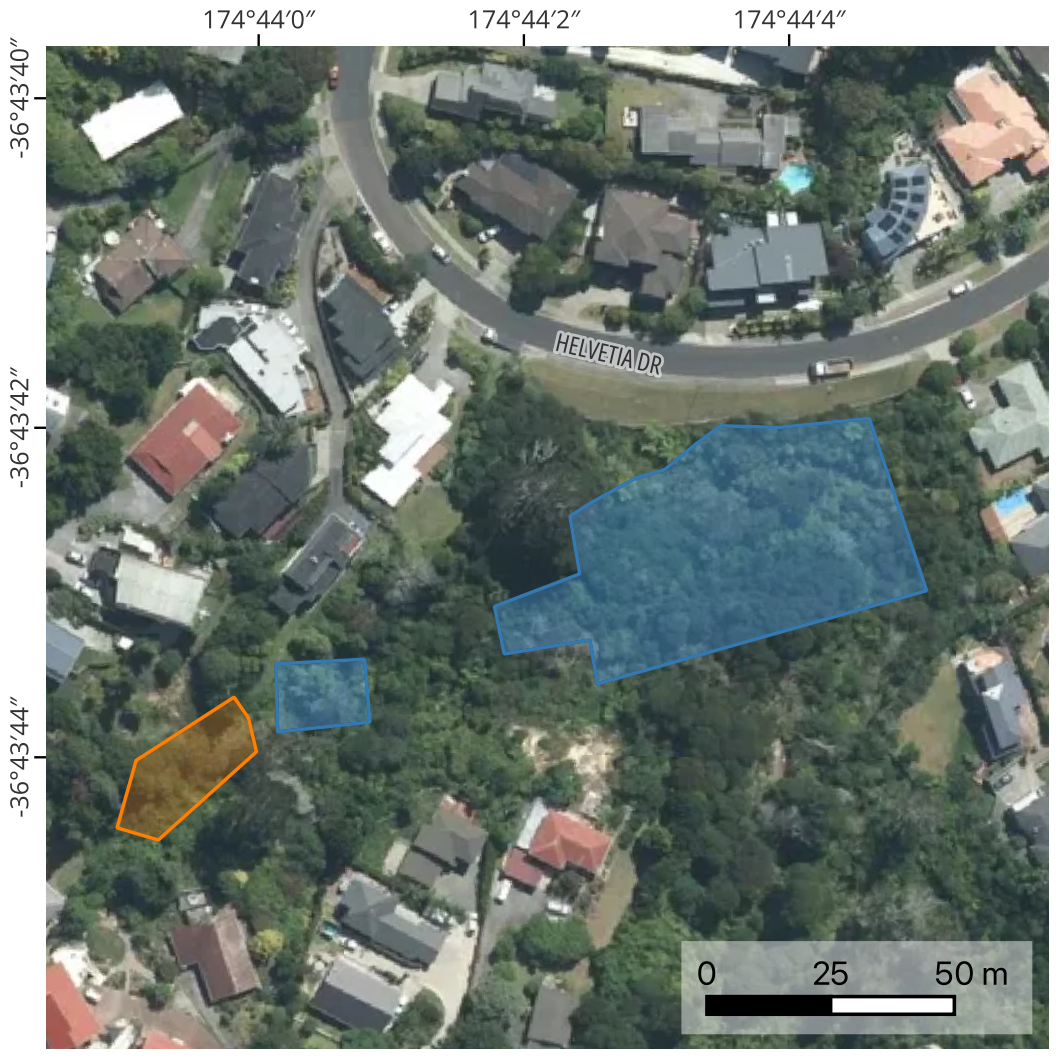
\includegraphics[keepaspectratio]{../2_1_figures/method/A3_sites_overview.png}}

}

\subcaption{\label{fig-sites_extent_A3}Bushglen Reserve (A3)}

\end{minipage}%
%
\begin{minipage}{0.50\linewidth}

\centering{

\pandocbounded{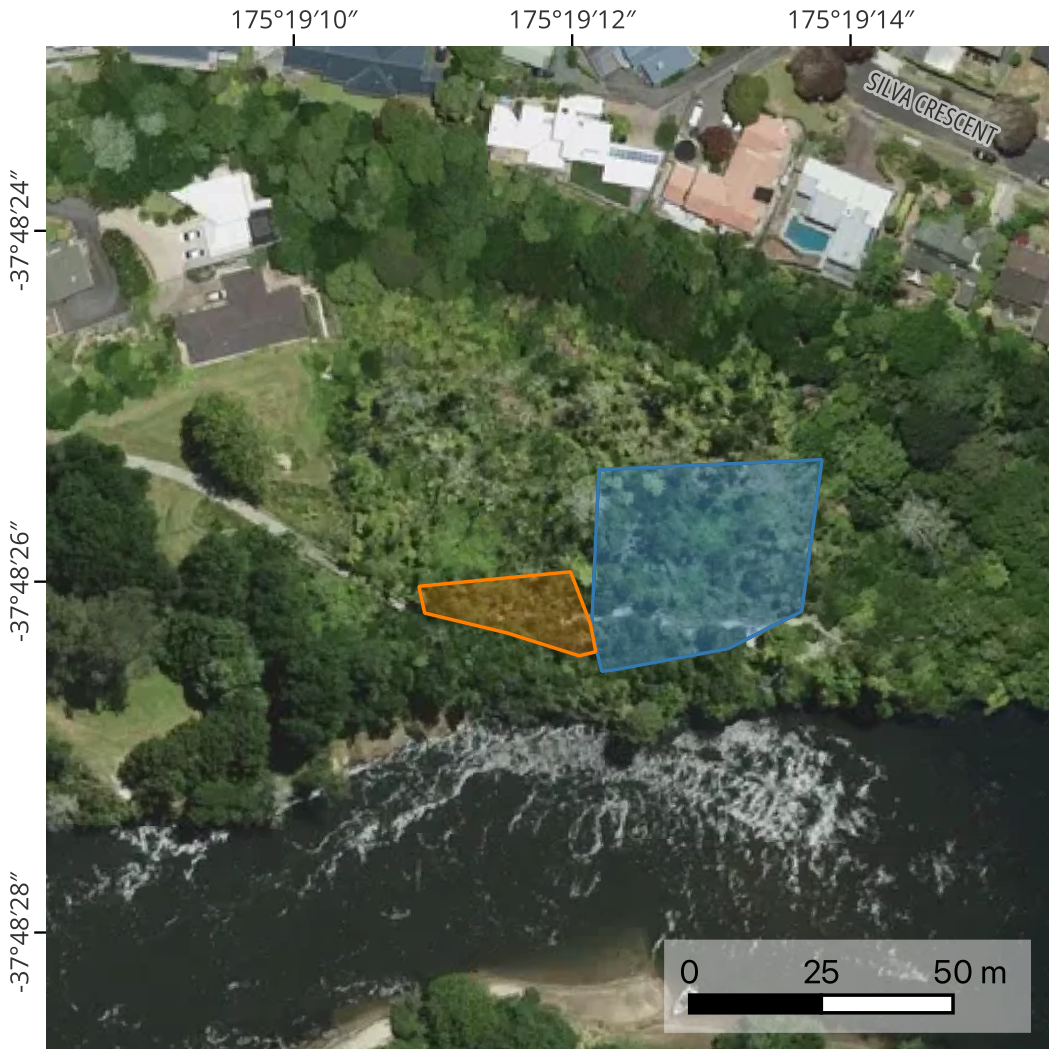
\includegraphics[keepaspectratio]{../2_1_figures/method/H1_sites_overview.png}}

}

\subcaption{\label{fig-sites_extent_H1}Hammond Park (H1)}

\end{minipage}%

\end{figure}%

}

\caption[Extent of training and
test-zones.]{\label{fig-sites_extent}Site extents showing training
(blue) and test (orange) zones used for model evaluation; maps showing
full park extent and surrounding area can be found in
\quartosfigref{sfig-sites_extent_overview}. Site areas are listed in
Table~\ref{tbl-overview}. Basemap: Copyright LINZ aerial imagery under
\href{https://creativecommons.org/licenses/by/4.0/}{CC BY 4.0}.}

\end{figure}%

\section{\texorpdfstring{\hyperref[acronyms_UAV]{UAV}-\hyperref[acronyms_RGB]{RGB}
and \hyperref[acronyms_MS]{MS} Data
Collection}{UAV-RGB and MS Data Collection}}\label{and-data-collection}

Flights were carried out with a \hyperref[acronyms_M3M]{DJI Mavic 3
Multispectral (\citeproc{ref-djiDJIMavic}{DJI, n.d.-a})}
\hyperref[acronyms_UAV]{UAV} (Figure~\ref{fig-M3M}), equipped with a
\hyperref[acronyms_RGB]{RGB} visible imaging sensor (20 MP, 5280 × 3956)
and a \hyperref[acronyms_MS]{MS} imaging sensor (5 MP, 2592 × 1944)
across four spectral bands: green (560±16 nm), red (650±16 nm), red edge
(730±16 nm), and near-infrared (860±26 nm). Initial
\hyperref[acronyms_RGB]{RGB} imagery and \hyperref[acronyms_MS]{MS}
imagery captures were conducted in April 2025 but had to be repeated due
to variable lighting conditions, resulting in poor data quality
(\quartosfigref{sfig-ms_seamline}). Final \hyperref[acronyms_RGB]{RGB}
imagery and \hyperref[acronyms_MS]{MS} imagery were acquired on 19
September (A1--A3) and 20 September (H1) 2025.

All flights were carried out under full sunlight with wind speeds below
6 m/s. To ensure optimal exposure, flights were conducted within two
hours of solar noon (\citeproc{ref-robbinsNatureScanRGB2025}{Robbins et
al., 2025}). Flight paths were automatically generated in DJI Pilot 2
(\citeproc{ref-djiDJIPilot}{DJI, n.d.-b}), and the
\hyperref[acronyms_RTK]{RTK} system was connected to the nearest
\hyperref[acronyms_GNSS]{GNSS} base station from
\hyperref[acronyms_PositioNZ]{Toitū Te Whenua PositioNZ Real Time
Service (PositioNZ-RT)} to ensure high positional accuracy. Flight
altitude was set to 50 m \hyperref[acronyms_AGL]{above ground
level (AGL)}, based on a 1 m \hyperref[acronyms_DEM]{digital elevation
model (DEM)}, corrected to the geoid
(\citeproc{ref-linzNZGeoid2012}{LINZ, 2012},
\citeproc{ref-linzNewZealand2025}{2025}). Forward and side overlap were
set to 85\%, and flight speed was specified at 3 m/s. These settings
were chosen and adapted based on the recommendations in Heim et al.
(\citeproc{ref-heimMultispectralAerial2019}{2019}). As suggested by
Olsson et al. (\citeproc{ref-olssonRadiometricCorrection2021}{2021}), a
photo of a MicaSense RP03 \hyperref[acronyms_CRP]{Calibrated Reference
Panel (CRP)} was taken after takeoff and before landing with all other
settings left at their defaults.

\section{\texorpdfstring{\hyperref[acronyms_UAV]{UAV}-\hyperref[acronyms_LiDAR]{LiDAR}
Data Collection}{UAV-LiDAR Data Collection}}\label{data-collection}

\hyperref[acronyms_LiDAR]{LiDAR} flights were carried out on 22 May 2025
using a DJI Matrice 350 RTK (\citeproc{ref-djiMatrice350}{DJI, n.d.-c})
equipped with a Zenmuse L2 sensor (Figure~\ref{fig-Matrice350}; DJI,
n.d.-e). The Zenmuse L2 is a \hyperref[acronyms_LiDAR]{LiDAR} sensor,
which emits laser impulses and measures the time for the laser pulse to
be reflected by obstacles (e.g.~vegetation, buildings or the ground) and
return to the sensor. The time is then converted to distance in the
given direction, which results in a three-dimensional point cloud.
Flight altitude was set to 60 m \hyperref[acronyms_AGL]{AGL} at A1 and
70 m \hyperref[acronyms_AGL]{AGL} at A2. The reduced flight height at
site A1 was chosen to maintain operational safety margins with a
co-occurring flight at this location. Each site included one nadir
flight and four (A1) or two (A2) oblique flights at a 20° angle
(Table~\ref{tbl-overview}). This difference in oblique flights was due
to operational limitations of carrying out flights in mixed urban-forest
environment to avoid overflight of private properties and comply with
regulations. Forward overlap was set to 80\%, side overlap to 50\%, and
flight speed to 7 m/s. Five returns were recorded per pulse, and the
scan mode was non-repetitive. The \hyperref[acronyms_RTK]{RTK} setup
mirrored that used for the
\hyperref[acronyms_MS]{MS}/\hyperref[acronyms_RGB]{RGB} imagery flights.
The point density was at 8630 points/m² for site A1 and 4116 points/m²
for site A2. The main reason for the difference in point density is the
number of oblique flights (Table~\ref{tbl-overview}), which results in
more overlapping flight paths and thus variable point density.
Furthermore, site A2 had a section with more open swampy areas, meaning
less vegetation and therefore further reduced point density.

\begin{figure}[H]

\centering{

\begin{figure}[H]

\begin{minipage}{0.49\linewidth}

\centering{

\pandocbounded{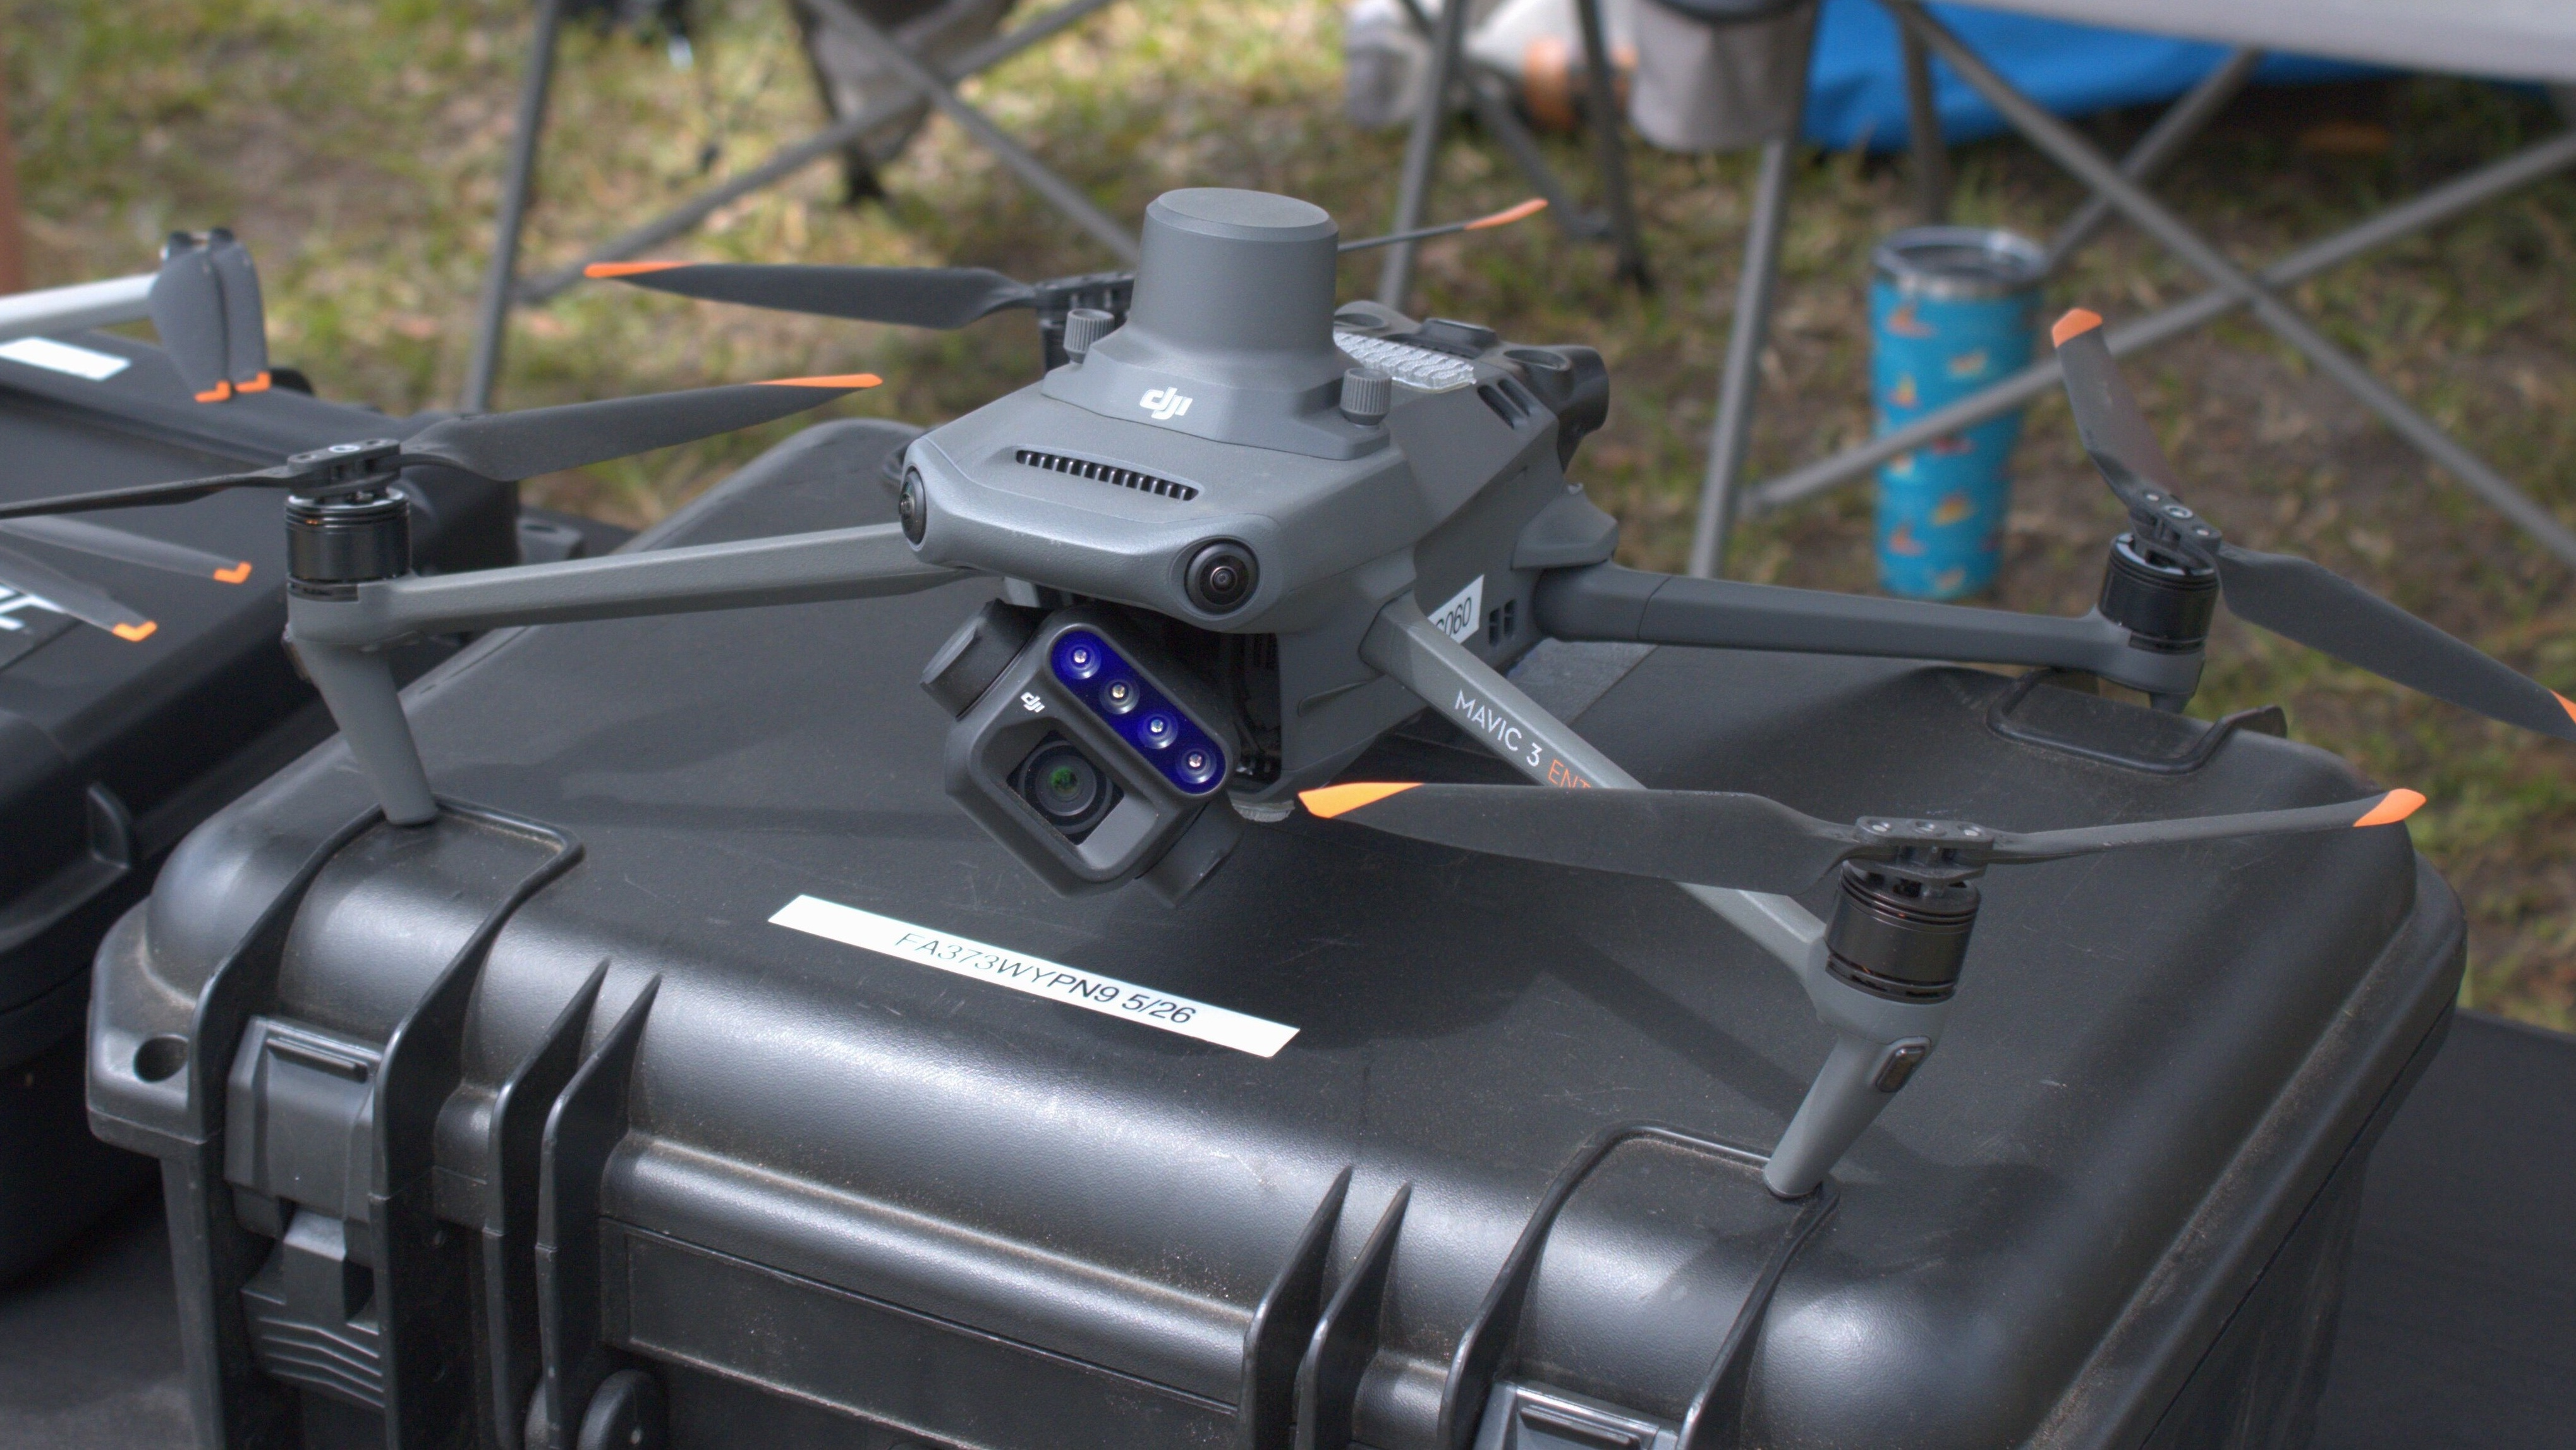
\includegraphics[keepaspectratio]{../2_1_figures/method/M3M.jpeg}}

}

\subcaption{\label{fig-M3M}The DJI Mavic 3 Multispectral
\hyperref[acronyms_UAV]{UAV} with the \hyperref[acronyms_RGB]{RGB} and
\hyperref[acronyms_MS]{MS} sensors. Image: From wikimedia by \emph{ZLEA}
(\citeproc{ref-zleaEnglishDJI2024}{2024}). CC-BY-SA-4.0.}

\end{minipage}%
%
\begin{minipage}{0.02\linewidth}
~\end{minipage}%
%
\begin{minipage}{0.49\linewidth}

\centering{

\pandocbounded{\includegraphics[keepaspectratio]{../2_1_figures/method/Matrice_350_AUT.JPG}}

}

\subcaption{\label{fig-Matrice350}The DJI Matrice 350
\hyperref[acronyms_UAV]{UAV}-platform equipped with the Zenmuse L2
\hyperref[acronyms_LiDAR]{LiDAR} sensor. Image: Copyright by Auckland
University of Technology (AUT). Reprinted with permission.}

\end{minipage}%

\end{figure}%

}

\caption[UAVs used for data collection.]{\label{fig-UAV}The two
\hyperref[acronyms_UAV]{UAVs} used for
\hyperref[acronyms_RGB]{RGB}/\hyperref[acronyms_MS]{MS} (\textbf{a}) and
\hyperref[acronyms_LiDAR]{LiDAR} (\textbf{b}) data collection.}

\end{figure}%

\subsection{Regulatory Compliance and Safety
Considerations}\label{regulatory-compliance-and-safety-considerations}

\hyperref[acronyms_UAV]{UAV}-flights were conducted in accordance with
\hyperref[acronyms_CAA]{Civil Aviation Authority (CAA)} Part 101
operation rules and in compliance with relevant local regulations. Prior
to each flight, operations were logged and approved via the
\href{https://pilot.airshare-utm.io/info}{Airshare} airspace management
platform. This was required, since all sites were located within the
control zone (CTR) airspace from Whenuapai Airport (A1-A3) or Hamilton
Airport (H1). When operations were conducted within 4km of an aerodrome,
approval was gained from all relevant aerdrome operators prior to any
\hyperref[acronyms_UAV]{UAV} flights (Figure~\ref{fig-Airzone}). For
site A1, flight paths were planned to avoid overflight of sensitive
areas, including a generous distance to a Horse paddock with animals
present and the Glenfield cemetery at Eskdale Reserve (A1).

\begin{figure}

\centering{

\begin{figure}[H]

\begin{minipage}{0.49\linewidth}

\centering{

\pandocbounded{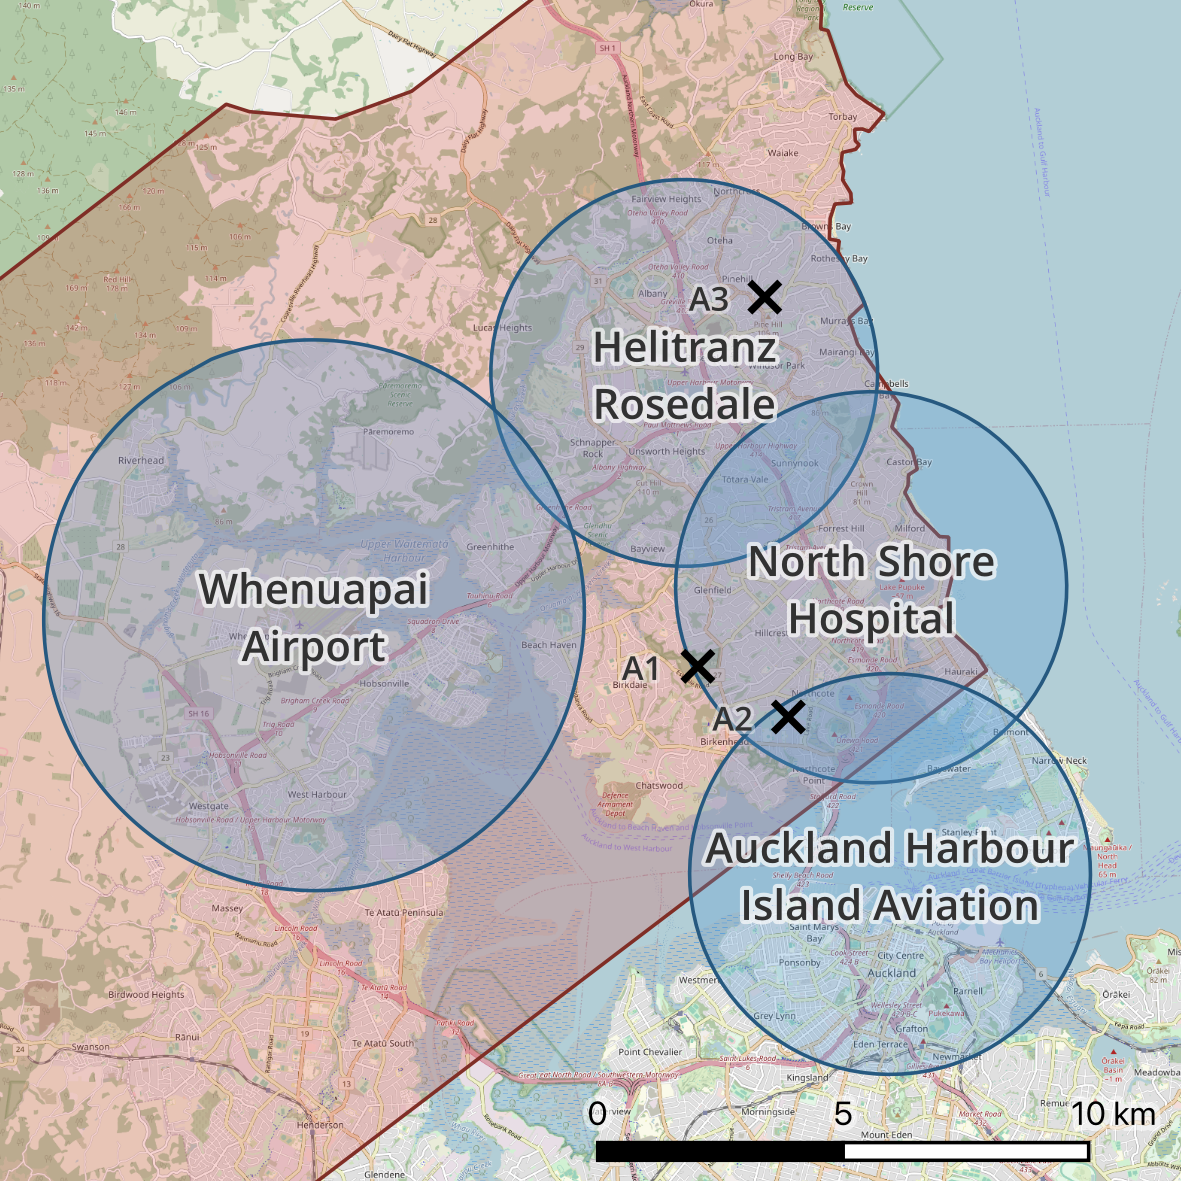
\includegraphics[keepaspectratio]{../2_1_figures/method/Auckland_Airzone.png}}

}

\subcaption{\label{fig-AKL_airzone}Auckland Airspace.}

\end{minipage}%
%
\begin{minipage}{0.02\linewidth}
~\end{minipage}%
%
\begin{minipage}{0.49\linewidth}

\centering{

\pandocbounded{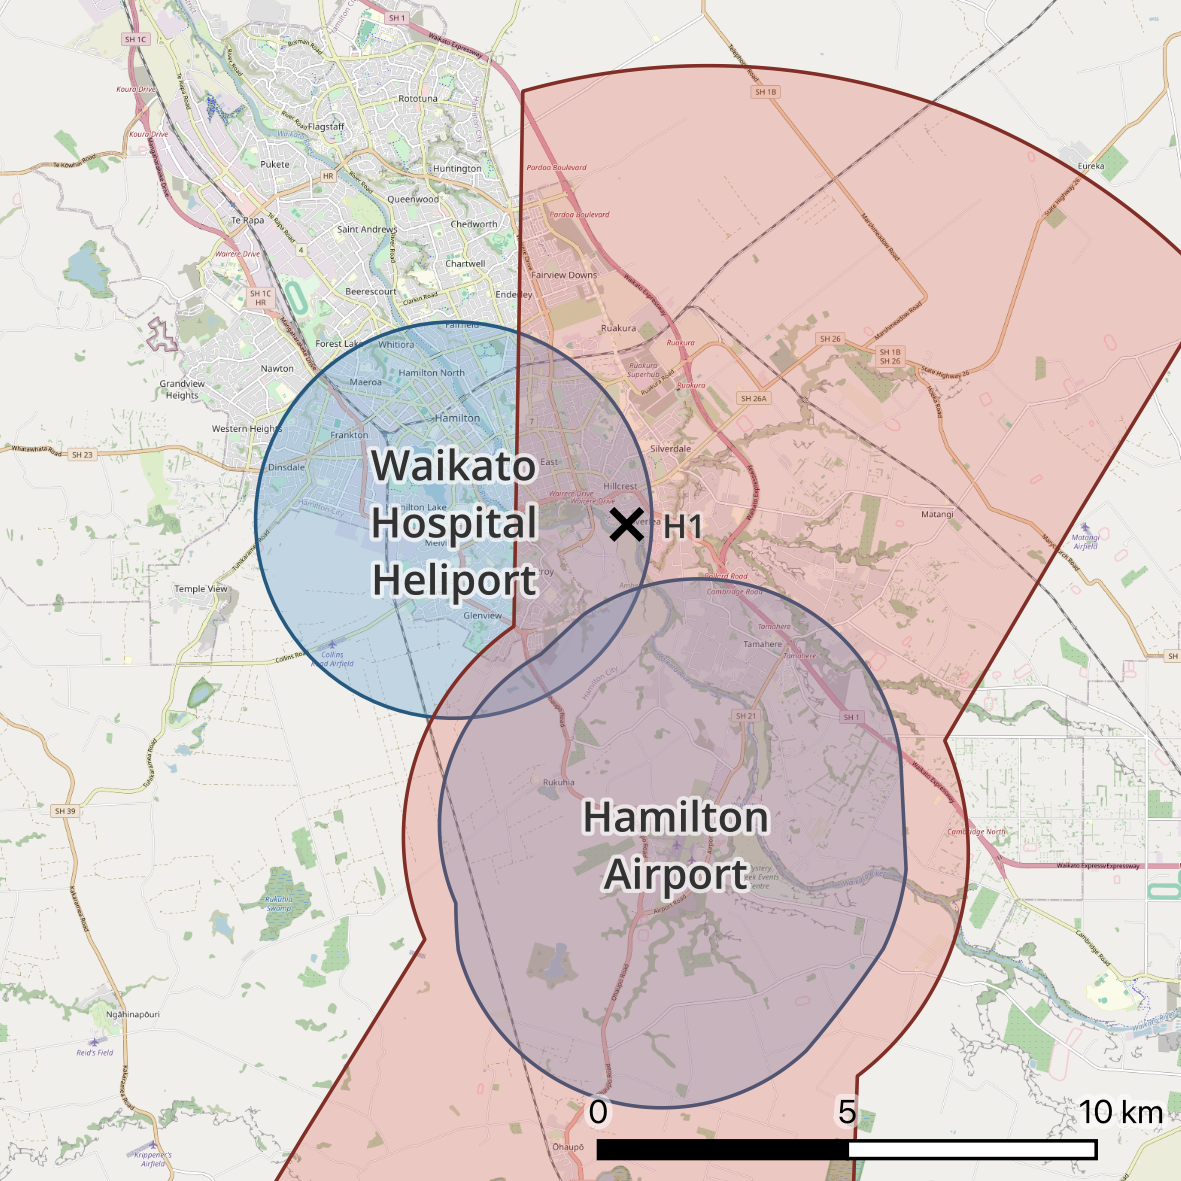
\includegraphics[keepaspectratio]{../2_1_figures/method/Hamilton_Airzone.png}}

}

\subcaption{\label{fig-HAM_airzone}Hamilton Airspace.}

\end{minipage}%

\end{figure}%

}

\caption[Airspace considerations.]{\label{fig-Airzone}The maps for
Auckland (\textbf{a}) and Hamilton (\textbf{b}) airspaces. Blue area
shows zones within 4km of an aerodrome and red are Control Zones. Black
crosses indicate research sites. All airspace boundaries are
approximations based on data from the New Zealand Aeronautical
Information Package (AIP) issued 25 December 2025. Basemap: Copyright
\href{https://www.openstreetmap.org}{OpenStreetMap} contributors under
\href{https://opendatacommons.org/licenses/odbl/}{ODbl} by
\href{https://osmfoundation.org/}{OSFM}.}

\end{figure}%

Landownership requirements were verified for all sites. As all locations
were on council-managed land (Auckland Council for A1--A3, Hamilton City
Council for H1), formal consent was not required
(\citeproc{ref-aucklandcouncilWhereyou}{Auckland Council, n.d.};
\citeproc{ref-hamiltoncitycouncilFlyingdrone}{Hamilton City Council,
n.d.}), except for one privately owned property boundary at Bushglen
Reserve (A3), for which verbal consent was obtained. A briefed observer
was present during all flight operations to maintain situational
awareness and ensure safe operations in these urban environments.

\section{Reference Data Collection}\label{reference-data-collection}

Ground-truthing of \hyperref[acronyms_SM]{\emph{S. maire}} on sites A2
and A3 was carried out on 10 May and 14 June 2025 for site A1.
\hyperref[acronyms_SM]{\emph{S. maire}} locations were shown by
volunteers from the local conservation group. To ensure exact
positioning, the \hyperref[acronyms_RS3]{Emlid Reach RS3 RTK receiver
(\citeproc{ref-emlidReachRS3}{Emlid, n.d.})} was used and connected to
the closest \hyperref[acronyms_PositioNZ]{PositioNZ-RT} base station.
The receiver was then connected to QField
(\citeproc{ref-qfield2024}{OPENGIS.ch}). In the field, the receiver was
positioned next to the trunk. Locations were only stored once the
receiver had a confirmed accuracy of \textless30 cm. When travelling
between sites, footwear was changed to reduce risk to spread
\hyperref[acronyms_AP]{\emph{A. psidii}} spores. Site H1 was not
ground-truthed with the receiver. Since all trees, except two, were
directly adjacent to the path, their rough locations were noted and
later identified on the orthomosaic.

\section{Data Processing and
Analysis}\label{data-processing-and-analysis}

All data processing and analysis was performed using a combination of
Python (v3.13.2), Agisoft Metashape
(\citeproc{ref-agisoftllcAgisoftMetashape2025a}{Agisoft LLC, v2.2.1,
2025}), DJI Terra (\citeproc{ref-djiDJITerra}{DJI, v4.13.3.0, n.d.}) and
CloudCompare
(\citeproc{ref-cloudcompareCloudCompareVersion2022}{CloudCompare,
v2.14.alpha, 2022}). Computations were carried out on a workstation with
a 13th Gen Intel® Core™ i7-13700 CPU, NVIDIA GeForce RTX 4070 Ti GPU,
and 128 GB RAM running Windows 11. The following sections describe the
data preprocessing, training and inference workflow in detail. The
source code of this thesis is available on
\href{https://www.github.com/pfaffrob/MSc_Thesis_RP}{www.github.com/pfaffrob/MSc\_Thesis\_RP}.

\subsection{Orthomosaic}\label{orthomosaic}

\hyperref[acronyms_RGB]{RGB} and \hyperref[acronyms_MS]{MS} orthomosaics
were generated from raw imagery in Agisoft Metashape, following
workflows proposed by Geospatial Tips
(\citeproc{ref-geospatialtipsAgisoftMetashape2022}{2022}), with some
modifications for our data requirements. This process involved first
calibrating reflectance and aligning of images, followed by iterative
tiepoint filtering based on reconstruction uncertainty (\textless27),
reprojection error (\textless0.83), and projection accuracy
(\textgreater3.8), with alignment optimisation after each step. A dense
point cloud was constructed and filtered by confidence (\textgreater2),
which was then used to build a 2.5D surface (a point cloud which is
triangulated into a mesh without overhang). The orthomosaics were
exported at 2.5 cm/pixel resolution for \hyperref[acronyms_MS]{MS}
imagery and 1.5 cm/pixel for \hyperref[acronyms_RGB]{RGB} imagery, with
blending mode disabled (Figure~\ref{fig-wf_orthomosaic}). The blending
mode was disabled to ensure that no smoothing or interpolation occurred
during the orthomosaic generation process, and only raw image values
were assigned to each pixel.

To enhance spectral discrimination, four normalised
\hyperref[acronyms_VI]{vegetation indices (VIs)} were computed from the
four-channel \hyperref[acronyms_MS]{MS} orthomosaics
(Table~\ref{tbl-indices}) and stretched from float32 to uint16 format
(-1--1 to 0--65535), which is a common approach to normalise data for
\hyperref[acronyms_DL]{deep learning}
(\citeproc{ref-wagnerUsingUnet2019}{Wagner et al., 2019}).
\hyperref[acronyms_NDVI]{NDVI} was calculated as a fundamental index
sensitive to vegetation health and chlorophyll content.
\hyperref[acronyms_RENDVI]{RENDVI} utilises both
\hyperref[acronyms_RE]{red edge (RE)} and
\hyperref[acronyms_NIR]{near-infrared (NIR)} channels to detect
vegetation stress and subtle canopy changes
(\citeproc{ref-simsRelationshipsleaf2002}{Sims \& Gamon, 2002}).
\hyperref[acronyms_REDVI]{REDVI} applies a similar normalised difference
approach but substitutes the \hyperref[acronyms_RE]{RE} channel for
\hyperref[acronyms_NIR]{NIR}, offering an alternative canopy response
measurement (\citeproc{ref-briechleClassificationTree2020}{Briechle et
al., 2020}). \hyperref[acronyms_NGRDI]{NGRDI}, derived from
\hyperref[acronyms_G]{green (G)} and \hyperref[acronyms_R]{red (R)}
channels, provides vegetation signal independent of
\hyperref[acronyms_NIR]{NIR}. These indices were selected because they
have shown potential for species identification where spectral
signatures are needed due to limited morphological features
(\citeproc{ref-barreroRGBmultispectral2018}{Barrero \& Perdomo, 2018};
\citeproc{ref-briechleClassificationTree2020}{Briechle et al., 2020}).

Due to saturation of the \hyperref[acronyms_R]{R} and
\hyperref[acronyms_G]{G} bands on the \hyperref[acronyms_CRP]{CRP} photo
(\quartosfigref{sfig-crp_hist}), \hyperref[acronyms_MS]{MS} imagery and
\hyperref[acronyms_VI]{VIs} were processed in two calibration schemes:
absolute (using the sun sensor and \hyperref[acronyms_CRP]{CRP}) and
relative (using only the sun sensor; Table~\ref{tbl-band-combinations}).
Absolute calibration adjusts for exposure differences between sites,
whilst relative calibration was retained to evaluate whether the burned
\hyperref[acronyms_CRP]{CRP} pixels (\quartosfigref{sfig-crp_hist}) used
for radiometric calibration influenced model performance. A burned pixel
means that it is assigned the maximum value (65535 in uint16 format),
which means that the pixel value does not represent the true reflectance
of the surface, but rather the maximum value that the sensor can record
with the specified exposure settings (\quartosfigref{sfig-exposure}).

\begin{longtable}[]{@{}
  >{\centering\arraybackslash}p{(\linewidth - 2\tabcolsep) * \real{0.6275}}
  >{\raggedright\arraybackslash}p{(\linewidth - 2\tabcolsep) * \real{0.3725}}@{}}
\caption{The formulas for the \hyperref[acronyms_VI]{VIs} used in this
thesis.}\label{tbl-indices}\tabularnewline
\toprule\noalign{}
\begin{minipage}[b]{\linewidth}\centering
Index Formula
\end{minipage} & \begin{minipage}[b]{\linewidth}\raggedright
Source
\end{minipage} \\
\midrule\noalign{}
\endfirsthead
\toprule\noalign{}
\begin{minipage}[b]{\linewidth}\centering
Index Formula
\end{minipage} & \begin{minipage}[b]{\linewidth}\raggedright
Source
\end{minipage} \\
\midrule\noalign{}
\endhead
\bottomrule\noalign{}
\endlastfoot
\hyperref[acronyms_NDVI]{NDVI} \(= \dfrac{NIR - R}{NIR + R}\) & Rouse Jr
et al. (\citeproc{ref-rousejrMonitoringvegetation1974}{1974}) \\
& \\
\hyperref[acronyms_RENDVI]{RENDVI} \(= \dfrac{NIR - RE}{NIR + RE}\) &
Gitelson \& Merzlyak
(\citeproc{ref-gitelsonSpectralReflectance1994}{1994}) \\
& \\
\hyperref[acronyms_REDVI]{REDVI} \(= \dfrac{RE - R}{RE + R}\) & Briechle
et al. (\citeproc{ref-briechleClassificationTree2020}{2020}) \\
& \\
\hyperref[acronyms_NGRDI]{NGRDI} \(= \dfrac{G - R}{G + R}\) & Tucker
(\citeproc{ref-tuckerRedphotographic1979}{1979}) \\
\end{longtable}

\begin{figure}[H]

\centering{

\pandocbounded{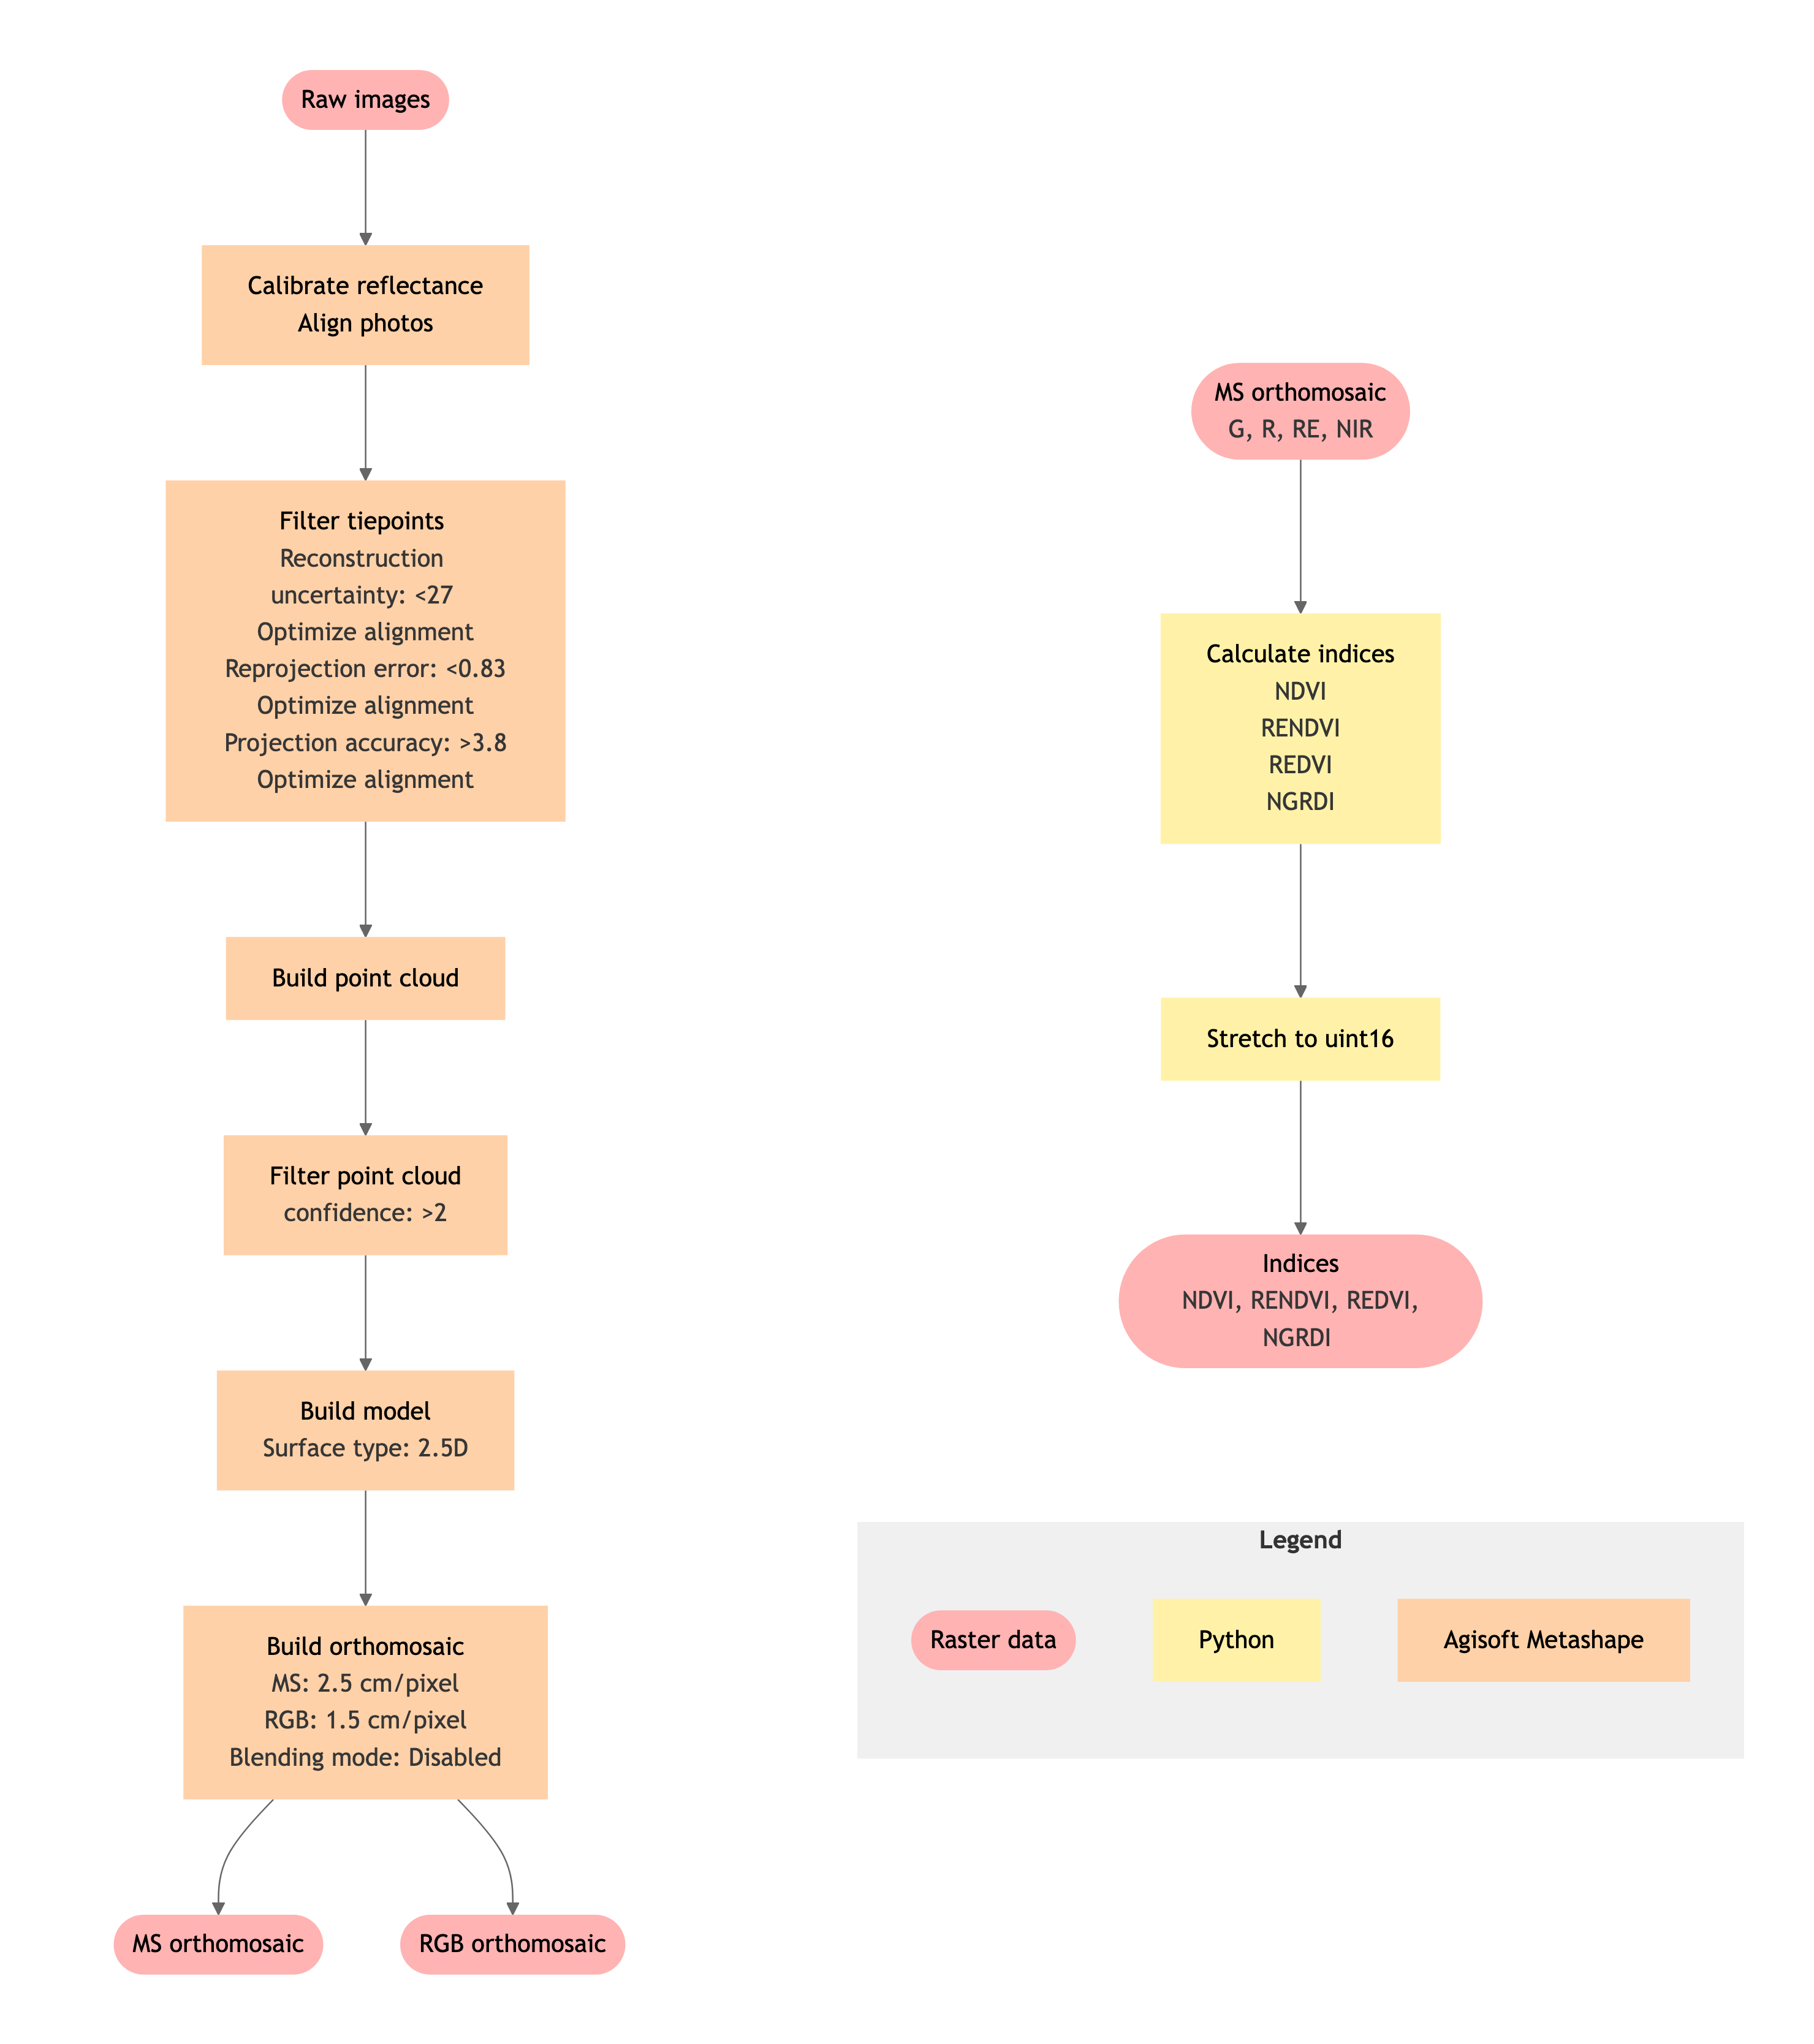
\includegraphics[keepaspectratio]{../2_1_figures/method/mermaid_orthomosaic.png}}

}

\caption[Orthomosaic generation
workflow.]{\label{fig-wf_orthomosaic}Workflow to generate the
orthomosaics and further processing to prepare for model input.}

\end{figure}%

\subsection{U-Net}\label{u-net}

\subsubsection{Annotation}\label{annotation}

Ground-truthed \hyperref[acronyms_SM]{\emph{S. maire}} locations were
overlaid on the orthomosaics. The annotator first examined unambiguous
\hyperref[acronyms_SM]{\emph{S. maire}} individuals to establish their
characteristic visual appearance. Using this visual knowledge base, the
visible canopy of each \hyperref[acronyms_SM]{\emph{S. maire}} instance
was digitised, which included more complex cases such as where visible
canopy was offset from the ground-truth point (e.g., due to trunk angle;
Figure~\ref{fig-label_offset_overgrowth}) or growth of other vegetation
within canopy (Figure~\ref{fig-label_other_vegetation}). Given the
limited training samples, dead foliage was excluded
(Figure~\ref{fig-label_dead}) to keep the training data as uniform as
possible and reduce within-class variability. Furthermore,
\hyperref[acronyms_SM]{\emph{S. maire}} present at ground-truth points
but with no visible canopy were not annotated
(Figure~\ref{fig-label_offset_overgrowth}). Where canopy crowns were
segmented by overlapping vegetation or shadowed/poorly lighted, only
areas clearly identifiable as \hyperref[acronyms_SM]{\emph{S. maire}}
were digitised, which could result in fragmented annotation polygons
(Figure~\ref{fig-label_other_vegetation}). To account for processing
differences and geometric offsets between sensors,
\hyperref[acronyms_RGB]{RGB} and \hyperref[acronyms_MS]{MS} imagery were
annotated independently. Following digitisation, annotation polygons
were rasterised to match orthomosaic resolution.

\begin{figure}

\centering{

\begin{figure}[H]

\begin{minipage}{0.49\linewidth}

\centering{

\pandocbounded{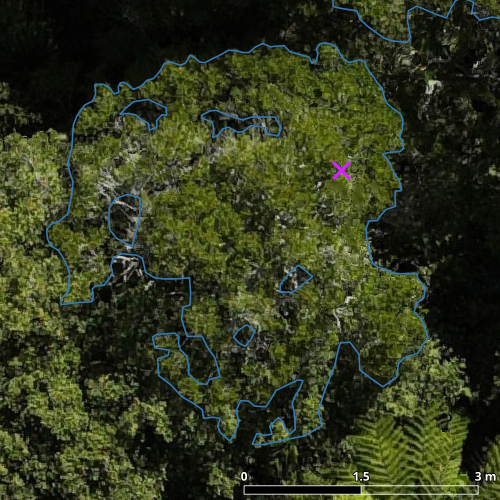
\includegraphics[keepaspectratio]{../2_1_figures/method/label-typical.png}}

}

\subcaption{\label{fig-label_typical}Typical
\hyperref[acronyms_SM]{\emph{S. maire}} canopy.}

\end{minipage}%
%
\begin{minipage}{0.02\linewidth}
~\end{minipage}%
%
\begin{minipage}{0.49\linewidth}

\centering{

\pandocbounded{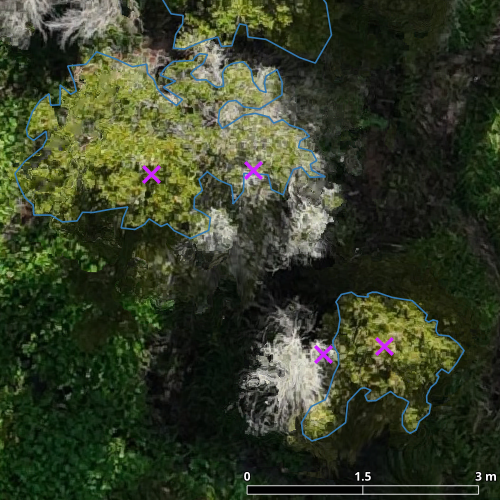
\includegraphics[keepaspectratio]{../2_1_figures/method/label-dead.png}}

}

\subcaption{\label{fig-label_dead}Exclusion of dead canopy from label.}

\end{minipage}%
\newline
\begin{minipage}{0.49\linewidth}

\centering{

\pandocbounded{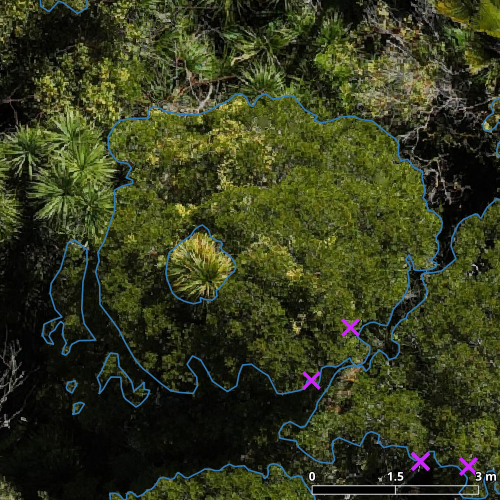
\includegraphics[keepaspectratio]{../2_1_figures/method/label-overgrowth.png}}

}

\subcaption{\label{fig-label_other_vegetation}Fragmented label and
growth ingrowth of other plant, presumably kiekie.}

\end{minipage}%
%
\begin{minipage}{0.02\linewidth}
~\end{minipage}%
%
\begin{minipage}{0.49\linewidth}

\centering{

\pandocbounded{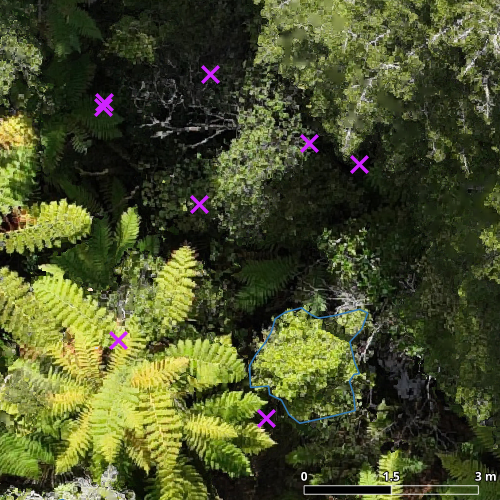
\includegraphics[keepaspectratio]{../2_1_figures/method/label-angle-undergrowth.png}}

}

\subcaption{\label{fig-label_offset_overgrowth}Canopy offset from the
ground-truthed position (bottom right) and overgrowth of other
vegetation.}

\end{minipage}%

\end{figure}%

}

\caption[Annotation examples.]{\label{fig-digitisation_examples}Examples
of \hyperref[acronyms_SM]{\emph{S. maire}} canopy annotation:
(\textbf{a}) typical crown, (\textbf{b}) canopy offset from the
ground-truth position with adjacent overgrowth, (\textbf{c}) dead canopy
excluded from annotation, and (\textbf{d}) fragmented annotation where
other vegetation grows within the crown. Annotation polygons are shown
in blue and ground-truth points as in pink.}

\end{figure}%

\subsubsection{Dataset Generation}\label{dataset-generation}

In \hyperref[acronyms_DL]{deep learning}, the optimisation of model
weights is based on the training data, while validation data is used
during training to monitor model performance on independent data and
prevent overfitting. Test data, in contrast, is used only for final
performance evaluation, ensuring an unbiased assessment of how the model
performs on unseen data (\citeproc{ref-ianDeepLearning2016}{Goodfellow
et al., 2016}). Therefore, to evaluate model performance, training,
validation, and test data must be separated carefully. This subset is
also required because the U-Net model cannot process these
full-resolution orthomosaics directly due to memory and computational
constraints, and must therefore be further divided into smaller chunks.
In geospatial applications, the partitioning is critical with tiling
frameworks where adjacent image tiles overlap and share boundary pixels.
If training and test data were derived from overlapping tiles within the
same area, performance metrics would be artificially inflated because
the model would have effectively ``seen'' the test data during training
(\citeproc{ref-kattenbornSpatiallyautocorrelated2022}{Kattenborn et al.,
2022}).

To avoid this bias, orthomosaics were cropped into two spatially
separated areas with zero overlap: a training zone and a test zone
(Table~\ref{tbl-overview}; Figure~\ref{fig-sites_extent}). Following the
tiling framework by Chen et al.
(\citeproc{ref-chenMultiInputChannel2024}{2024}), train and test zones
were clipped into 576x576 pixel tiles with 25\% overlap. The tiles of
the training zone were then further separated into a 80/20
train/validation split
(\citeproc{ref-kattenbornConvolutionalNeural2019}{Kattenborn et al.,
2019}). The selection was not fully random to ensure similar proportion
of \hyperref[acronyms_SM]{\emph{S. maire}} pixels in both subsets. The
resulting dataset exhibited severe class imbalance, with
\hyperref[acronyms_SM]{\emph{S. maire}} representing 3.4±0.7\% (mean±SE)
of pixels in training tiles and 4.9 ± 0.5\% in validation tiles
(\quartostblref{stbl-class_distribution}). Datasets with seven band
combinations were created to assess their relative performance
(Table~\ref{tbl-band-combinations}).

\begin{longtable}[]{@{}
  >{\raggedright\arraybackslash}p{(\linewidth - 4\tabcolsep) * \real{0.2264}}
  >{\raggedright\arraybackslash}p{(\linewidth - 4\tabcolsep) * \real{0.3585}}
  >{\raggedright\arraybackslash}p{(\linewidth - 4\tabcolsep) * \real{0.4151}}@{}}
\caption{Band combinations used for training with mirroring relative and
absolute combination for \hyperref[acronyms_MS]{MS}
bands.}\label{tbl-band-combinations}\tabularnewline
\toprule\noalign{}
\begin{minipage}[b]{\linewidth}\raggedright
Band Type
\end{minipage} & \begin{minipage}[b]{\linewidth}\raggedright
Bands
\end{minipage} & \begin{minipage}[b]{\linewidth}\raggedright
Description
\end{minipage} \\
\midrule\noalign{}
\endfirsthead
\toprule\noalign{}
\begin{minipage}[b]{\linewidth}\raggedright
Band Type
\end{minipage} & \begin{minipage}[b]{\linewidth}\raggedright
Bands
\end{minipage} & \begin{minipage}[b]{\linewidth}\raggedright
Description
\end{minipage} \\
\midrule\noalign{}
\endhead
\bottomrule\noalign{}
\endlastfoot
RGB & \hyperref[acronyms_RGB]{red-green-blue (RGB)} & Standard RGB
channels \\
MS\(_{rel}\) & \hyperref[acronyms_R]{R}, \hyperref[acronyms_G]{G},
\hyperref[acronyms_RE]{RE}, \hyperref[acronyms_NIR]{NIR} &
\hyperref[acronyms_MS]{MS} with relative calibration \\
MS\(_{abs}\) & \hyperref[acronyms_R]{R}, \hyperref[acronyms_G]{G},
\hyperref[acronyms_RE]{RE}, \hyperref[acronyms_NIR]{NIR} &
\hyperref[acronyms_MS]{MS} with absolute calibration \\
IND\(_{rel}\) & \hyperref[acronyms_NDVI]{NDVI},
\hyperref[acronyms_NGRDI]{NGRDI}, \hyperref[acronyms_REDVI]{REDVI},
\hyperref[acronyms_RENDVI]{RENDVI} & Vegetation indices \\
IND\(_{abs}\) & \hyperref[acronyms_NDVI]{NDVI},
\hyperref[acronyms_NGRDI]{NGRDI}, \hyperref[acronyms_REDVI]{REDVI},
\hyperref[acronyms_RENDVI]{RENDVI} & Vegetation indices \\
MS+IND\(_{rel}\) & \hyperref[acronyms_R]{R}, \hyperref[acronyms_G]{G},
\hyperref[acronyms_RE]{RE}, \hyperref[acronyms_NIR]{NIR},
\hyperref[acronyms_RENDVI]{RENDVI} & MS\(_{rel}\) +
\hyperref[acronyms_RENDVI]{RENDVI}\(_{rel}\) \\
MS+IND\(_{abs}\) & \hyperref[acronyms_R]{R}, \hyperref[acronyms_G]{G},
\hyperref[acronyms_RE]{RE}, \hyperref[acronyms_NIR]{NIR},
\hyperref[acronyms_RENDVI]{RENDVI} & MS\(_{abs}\) +
\hyperref[acronyms_RENDVI]{RENDVI}\(_{abs}\) \\
\end{longtable}

\subsubsection{Data Augmentation}\label{data-augmentation}

To improve model generalisation and mitigate the drawbacks of limited
training data, the dataset was artificially expanded by augmenting the
image tiles using Albumentations
(\citeproc{ref-buslaevAlbumentationsFast2020}{Buslaev et al., 2020}).
Augmentations included horizontal and vertical flips (probability 0.5),
geometric transformations via ShiftScaleRotate with ±10\% translation,
±15\% scale, and ±45° rotation (probability 0.5), grid distortion to
handle terrain and canopy variations (probability 0.2), and
multiplicative noise to simulate illumination changes (multipliers
0.95--1.05, probability 0.2). This approach applied only n-channel-safe
augmentations whilst creating substantial variation in training samples.

\subsubsection{Architecture}\label{architecture}

The U-Net \hyperref[acronyms_CNN]{CNN} architecture was selected for
semantic segmentation based on its established efficacy in
\hyperref[acronyms_RS]{remote sensing} applications for vegetation
detection (\citeproc{ref-abreu-diasAdvancesAutomated2025}{Abreu-Dias et
al., 2025}; \citeproc{ref-freudenbergLargeScale2019}{Freudenberg et al.,
2019}; \citeproc{ref-kattenbornConvolutionalNeural2019}{Kattenborn et
al., 2019}; \citeproc{ref-lobotorresApplyingFully2020}{Lobo Torres et
al., 2020}; \citeproc{ref-shahiDeepLearningBased2023}{Shahi et al.,
2023}). The model follows an encoder-decoder structure with skip
connections (\citeproc{ref-ronnebergerUNetConvolutional2015}{Ronneberger
et al., 2015}). In the contracting path, two 3×3 convolutions followed
by a \hyperref[acronyms_ReLU]{rectified linear unit (ReLU)} activation
are applied, then a 2×2 max pooling operation with stride 2 downsamples
by halving spatial resolution whilst doubling feature channels. This
pattern repeats through four encoder blocks. The expanding path mirrors
this: a 2×2 transposed convolution upsamples the feature map and halves
the channels, and is merged with its corresponding feature map from the
contracting path through skip connections that preserve spatial detail.
Two 3×3 convolutions and \hyperref[acronyms_ReLU]{ReLU} activations
follow, continuously reconstructing spatial resolution. A final 1×1
convolution maps each feature vector to output classes, producing the
segmentation map. The architecture is displayed in
Figure~\ref{fig-unet}.

The implementation was adjusted by adding zero-padding to the 3×3
conv/\hyperref[acronyms_ReLU]{ReLU} blocks to retain input-to-output
spatial resolution, eliminating the cropping required in the original
design and simplifying inference post-processing. Whilst zero-padding
could introduce artefacts at tile boundaries
(\citeproc{ref-huangTilingstitching2019}{Huang et al., 2019}), this was
not observed with the applied tiling approach. Therefore, other options,
such as using a buffer for predictions which is clipped post-processing
(\citeproc{ref-ballAccuratedelineation2023}{Ball et al., 2023};
\citeproc{ref-freudenbergLargeScale2019}{Freudenberg et al., 2019}),
were not further explored. The model was implemented in PyTorch
(\citeproc{ref-paszkePyTorchImperative2019}{Paszke et al., 2019}) and
core functionalities used from Pfaff
(\citeproc{ref-pfaffPrivetdetectionunpublished}{unpublished}).

\begin{figure}

\centering{

\pandocbounded{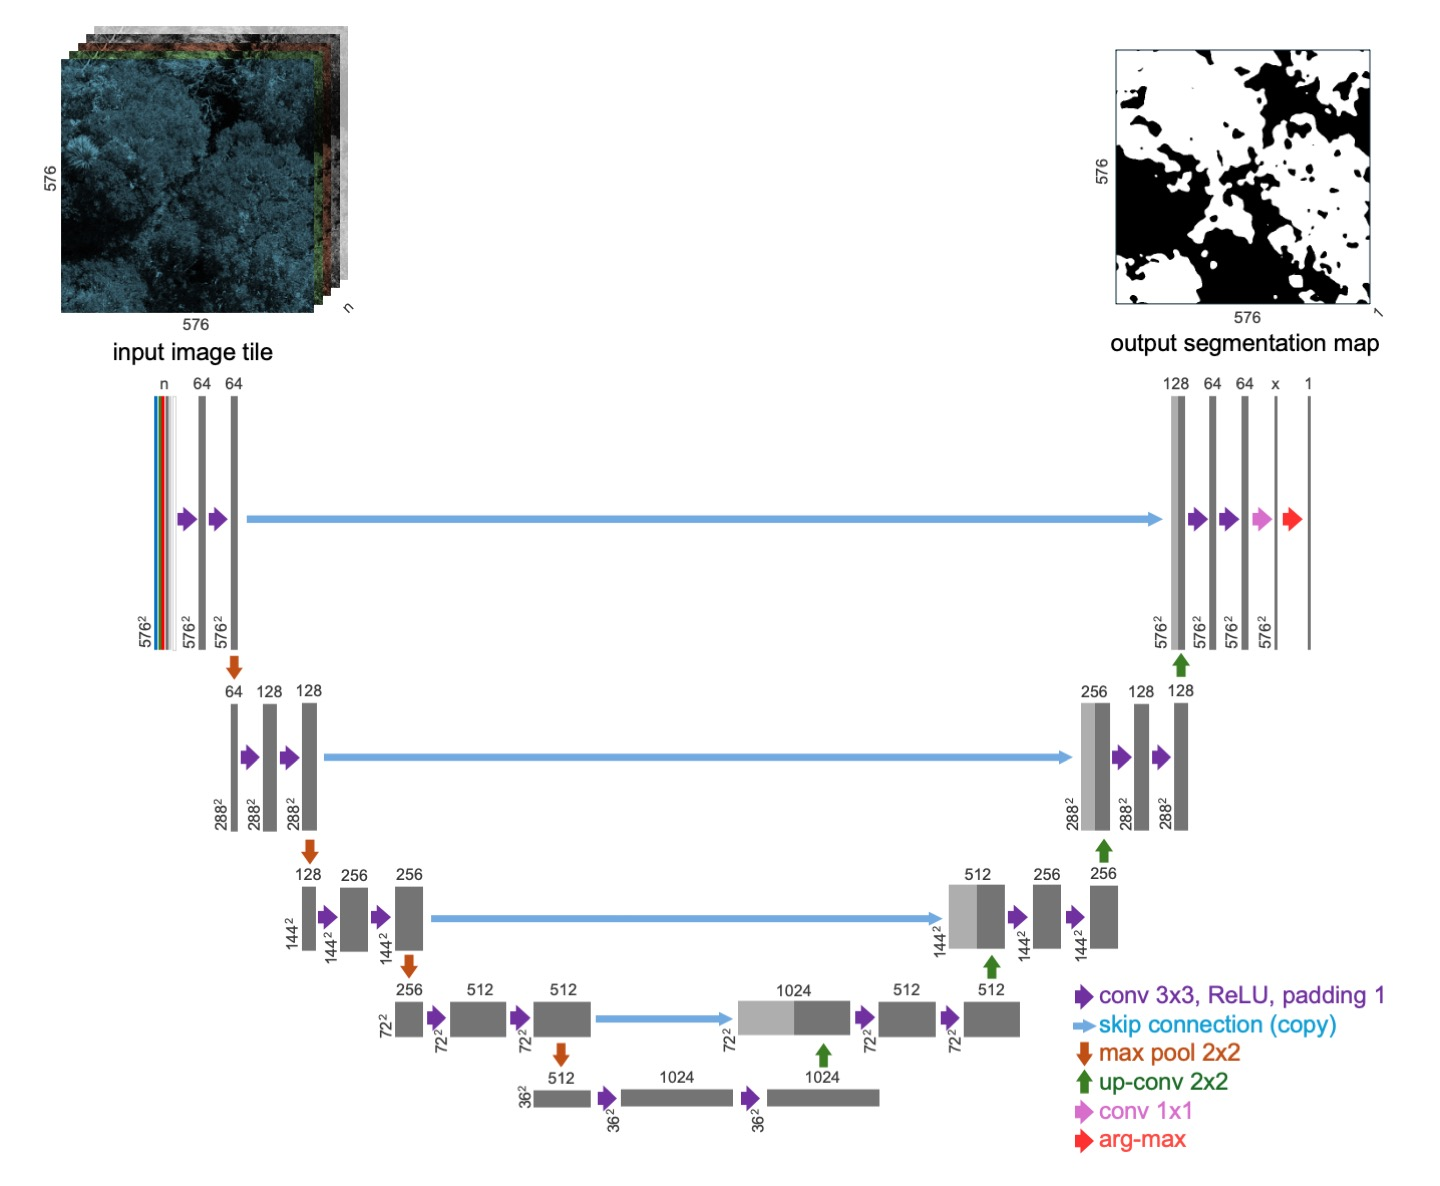
\includegraphics[keepaspectratio]{../2_1_figures/unet.jpg}}

}

\caption[U-Net architecture.]{\label{fig-unet}U-Net architecture which
accepts n-channels input image of 576×576 pixels. Each grey box
represents a multichannel feature map. Channel numbers are shown on top
of each box, with spatial resolution indicated at the lower left. Light
grey boxes display feature map copies, and arrows represent the various
operations.}

\end{figure}%

\subsubsection{Loss Functions}\label{loss-functions}

Selection of a suitable loss function is critical for training a
\hyperref[acronyms_DL]{deep learning} model
(\citeproc{ref-azadLossFunctions2023}{Azad et al., 2023}). The loss
function calculates the error between the annotation mask and the
predicted output, thereby guiding the optimisation of network weights
during training. Various loss functions are used in binary semantic
segmentation to address different challenges, such as the class
imbalanced present in this study (target class representing only
3.4±0.7\% (mean±SE) of pixels; \quartostblref{stbl-class_distribution}).
Such a class imbalance has been identified as a crucial factor
influencing \hyperref[acronyms_DL]{deep learning} model performance
(\citeproc{ref-ghoshclassimbalance2024}{Ghosh et al., 2024}). Selecting
a loss function which applies class weighting is a common mitigation
strategy (\citeproc{ref-bourdayComparativeStudy2024}{Bourday et al.,
2024}). Given the importance of this selection, three loss functions
were evaluated: \hyperref[acronyms_WBCE]{\(L_{WBCE}\)} with class
weights of 1, 10, and 50; unweighted
\hyperref[acronyms_DICE]{\(L_{Dice}\)} loss; and
\hyperref[acronyms_WBCE_D]{\(L_{c}\)}, a combination of the two, which
has shown good results in imbalanced binary segmentation tasks
(\citeproc{ref-koishiyevaAnalysisLoss2025}{Koishiyeva et al., 2025}).

In the following formulations, \(y^{(i)}\) denotes the ground-truth
label for pixel \(i\) (0 = background, 1 = target class). The model's
predicted probability for that pixel is represented by
\(\hat{y}^{(i)}\). Additionally, \(N\) indicates the total number of
pixels, and \(\beta\) is the weight assigned to the target class.

\hyperref[acronyms_WBCE]{\(L_{WBCE}\)} adjusts the standard binary
cross-entropy loss by applying a target class-specific weight
(\(\beta\)), increasing the penalty for misclassifying minority class
pixels (\citeproc{ref-liCombinedLossBased2022}{Li et al., 2022}):

\begin{equation}\phantomsection\label{eq-WBCE}{
L_{WBCE} = - \sum_{i=0}^{N} \beta\, y^{(i)} \log\hat{y}^{(i)}
+ \big(1 - y^{(i)}\big)\, \log\big(1 - \hat{y}^{(i)}\big)
}\end{equation}

\hyperref[acronyms_DICE]{\(L_{Dice}\)} is a region-based overlap
optimisation loss function that is less sensitive to class imbalance, as
it directly optimises the overlap between predicted and ground-truthed
regions:

\begin{equation}\phantomsection\label{eq-Dice}{
L_{Dice} = 1 - \frac{2\, y^{(i)} \hat{y}^{(i)}}{y^{(i)} + \hat{y}^{(i)}}
}\end{equation}

The combined \hyperref[acronyms_WBCE_D]{\(L_{c}\)} loss function
balances pixel-wise accuracy with region overlap optimisation
(\citeproc{ref-liCombinedLossBased2022}{Li et al., 2022}):

\begin{equation}\phantomsection\label{eq-WBCE_D}{
L_{C} = L_{WBCE} + L_{Dice}
}\end{equation}

\subsubsection{Training Configuration}\label{training-configuration}

Separate models were trained on each site independently (single-site)
and on all sites combined (multi-site). The main limitation of
site-specific models is that they cannot be deployed to new locations.
This means that either a new model must be trained for each location
(requiring time-expensive ground-truthing and re-annotation, defeating
the purpose of a method aimed at identification of unknown
\hyperref[acronyms_SM]{\emph{S. maire}} locations), or a single model
must be developed that generalises across sites. Therefore, a single
model was trained on combined data from all four sites to assess whether
comparable or better performance could be achieved relative to
site-specific models.

For model training, \hyperref[acronyms_SGD]{stochastic gradient
descent (SGD)} optimisation with initial
\hyperref[acronyms_LR]{learning rates (LRs)} of 0.02 or
5×10\textsuperscript{-5} were used. A ReduceLROnPlateau scheduler
monitored target class \hyperref[acronyms_IoU]{intersection over
union (IoU)} on the validation split, reducing the
\hyperref[acronyms_LR]{LR} by a factor of 0.5 after 15 epochs without
improvement (\citeproc{ref-srivastavaAdvancingMultiClass2024}{Srivastava
et al., 2024}). Training ran for a maximum of 300 epochs with batch size
of 2 and early stopping after 20 epochs without improvement in training
loss. The best-performing model (by highest \hyperref[acronyms_F1]{F1}
on the validation dataset) was used for subsequent inference.

For single-site models, all combinations of \hyperref[acronyms_LR]{LRs}
(0.02, 5×10\textsuperscript{-5}), class weights (1, 10, 50), loss
functions (Dice, \hyperref[acronyms_WBCE]{\(L_{WBCE}\)},
\hyperref[acronyms_WBCE_D]{\(L_{c}\)}), and band combinations
(MS\(_{rel}\), RGB) were evaluated individually on each reserve. For the
remaining band combinations, base hyperparameters were used (weight=10,
\hyperref[acronyms_LR]{LR}=0.02,
loss=\hyperref[acronyms_WBCE_D]{\(L_{c}\)}), resulting in 120
single-site models.

For multi-site models trained on all available training data,
\hyperref[acronyms_LR]{LR} was set to 0.02. Three hyperparameter
combinations were tested across five band combinations (MS\(_{abs}\),
MS\(_{rel}\), MS\(_{abs}\) + RENDVI, IND\(_{abs}\),
\hyperref[acronyms_RGB]{RGB}), with unweighted
\hyperref[acronyms_DICE]{\(L_{Dice}\)},
\hyperref[acronyms_WBCE_D]{\(L_{c}\)} with weights 10 and 50, resulting
in 15 multi-site models.

\subsubsection{Inference and Evaluation}\label{inference-and-evaluation}

Predictions were generated by applying identical preprocessing steps as
applied to the training zone (Figure~\ref{fig-sites_extent}) and running
the trained model in inference mode. Predicted tiles were stitched back
into a single orthomosaic, combining overlapping regions. In the
stitching process, any pixel predicted as target class was retained as
target class in the final output.

Model performance was evaluated on the spatially separated test zone
(Figure~\ref{fig-sites_extent}) to ensure metrics reflected unseen data.
The following evaluation metrics were calculated exclusively for the
target class. Precision, which measures the proportion of correctly
predicted target pixels among all pixels predicted as target:

\begin{equation}\phantomsection\label{eq-precision}{
\text{precision} = \frac{\text{TP}}{\text{TP} + \text{FP}}
}\end{equation}

where TP is true positives and FP is false positives. Recall measures
the proportion of correctly predicted target pixels among all actual
target pixels:

\begin{equation}\phantomsection\label{eq-recall}{
\text{recall} = \frac{\text{TP}}{\text{TP} + \text{FN}}
}\end{equation}

where FN is false negatives. The primary aggregating metric was
\hyperref[acronyms_F1]{F1}, the harmonic mean of precision and recall:

\begin{equation}\phantomsection\label{eq-F1}{
\text{F1} = 2 \times \frac{\text{precision} \times \text{recall}}{\text{precision} + \text{recall}}
}\end{equation}

To assess whether additional \hyperref[acronyms_SM]{\emph{S. maire}}
canopy area improves model performance, a Pearson correlation test was
performed between annotated area of the training zones and
\hyperref[acronyms_F1]{F1} scores. The hypotheses were defined as
\(H_0\): increasing available \hyperref[acronyms_SM]{\emph{S. maire}}
canopy area does not improve model performance (no linear relationship),
and \(H_1\): increasing available \hyperref[acronyms_SM]{\emph{S.
maire}} canopy area improves model performance (positive linear
relationship). A simple linear regression was also fitted to quantify
the relationship.

\section{LiDAR Tree Segmentation}\label{lidar-tree-segmentation}

Two methods of \hyperref[acronyms_LiDAR]{LiDAR} based tree segmentation
were trialled to determine whether they could supplement the raster
based \hyperref[acronyms_FCNN]{FCNN} workflow: TreeLearn, which is
\hyperref[acronyms_DL]{deep learning}-based
(\citeproc{ref-henrichTreeLearndeep2024}{Henrich et al., 2024}), and
Treeiso, which is graph-based (\citeproc{ref-xi3DGraphBased2022}{Xi \&
Hopkinson, 2022}). Due to time constraints and preliminary assessment of
segmentation results indicating challenges with segmentation accuracy
(Figure~\ref{fig-tree_instance_seg}), these approaches were only
assessed qualitatively to determine whether they are worth exploring
further in future work. The following describes the processing steps
undertaken, and the workflow is shown in Figure~\ref{fig-wf_treeseg}.

\begin{figure}

\centering{

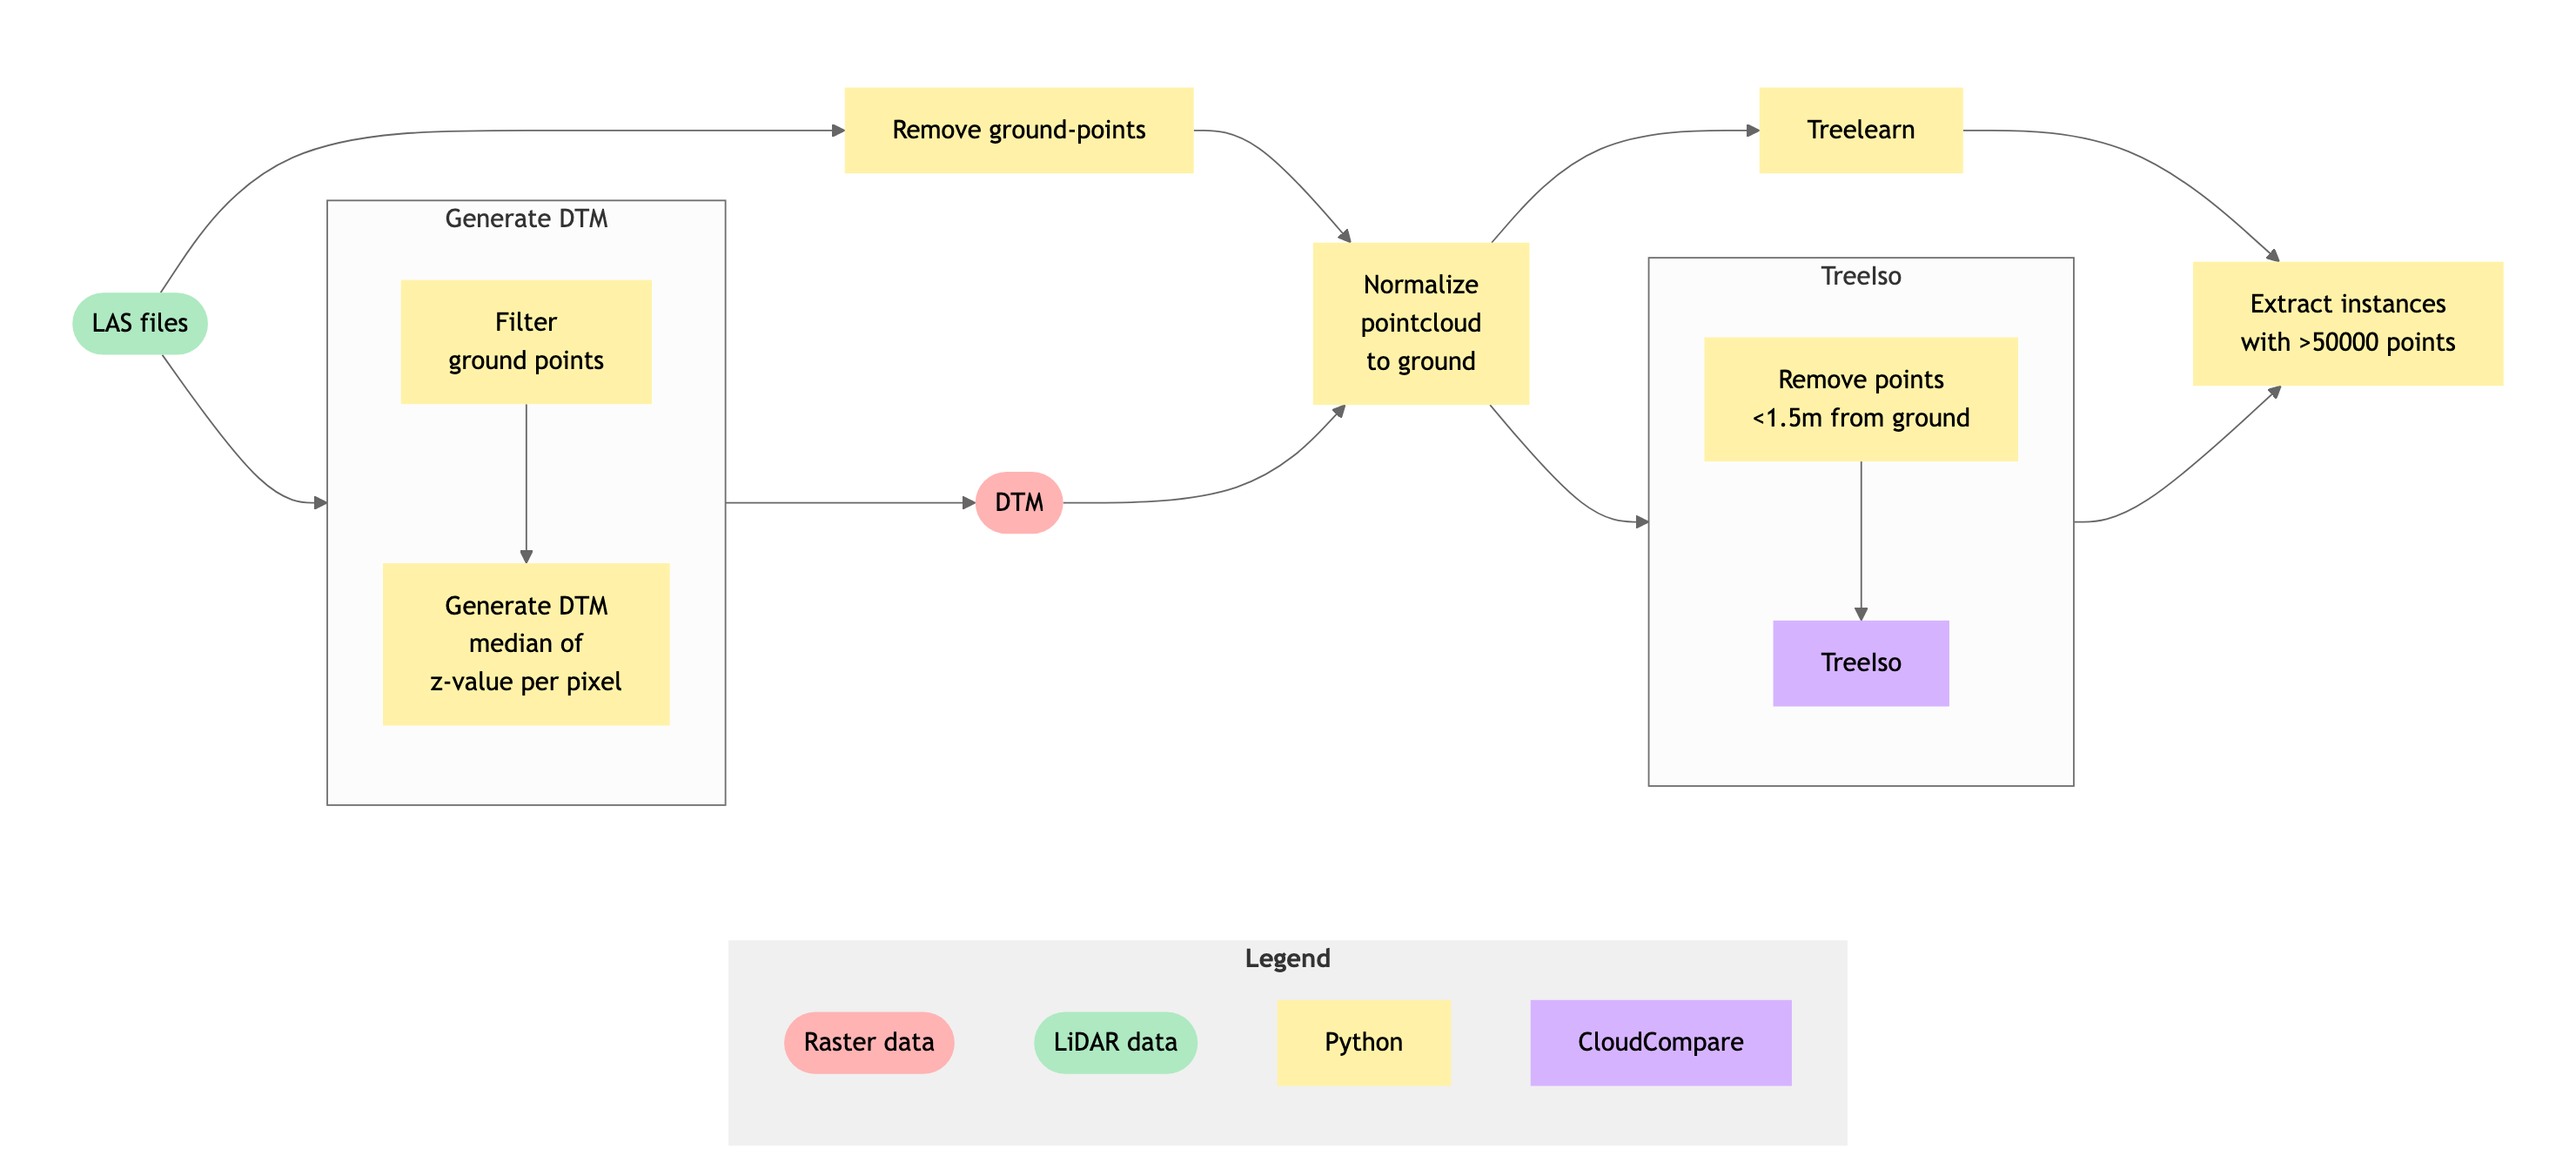
\includegraphics[width=6.5in,height=2.92in]{complete_thesis_files/figure-latex/mermaid-figure-2.png}

}

\caption[LiDAR tree segmentation
workflow.]{\label{fig-wf_treeseg}Workflow to test the LiDAR tree
segmentation methods (TreeLearn and Treeiso). This included point cloud
processing, including the generation of a DTM, and application of the
two segmentation methods.}

\end{figure}%

\subsection{Point Cloud Processing}\label{point-cloud-processing}

Raw \hyperref[acronyms_LiDAR]{LiDAR} data was processed to
\hyperref[acronyms_LAS]{LAS} files using DJI Terra. A 10cm
\hyperref[acronyms_DTM]{digital terrain model (DTM)} was generated from
the point cloud to enable height normalisation. Point clouds were
filtered to non-ground points and then normalised to ground level by
subtracting the \hyperref[acronyms_DTM]{DTM} elevation from each point's
z-coordinate. This ensured the height above ground level of the
represented vegetation structure rather than terrain elevation. For
Treeiso segmentation, points lower than 1.5 m above the ground were
removed to reduce noise from dense understory vegetation
(\citeproc{ref-xi3DGraphBased2022}{Xi \& Hopkinson, 2022}).

\subsection{Segmentation Methods}\label{segmentation-methods}

Both TreeLearn and Treeiso algorithms were applied to segment individual
tree crowns from the normalised point clouds. TreeLearn voxelises the
point cloud by dividing the 3D space into small cubes (voxels) and
assigning points to these cubes, then applying a
\hyperref[acronyms_DL]{deep learning} model to classify each voxel as
belonging to a specific tree instance, effectively segmenting individual
tree crowns based on learned spatial features and patterns in the point
cloud data (\citeproc{ref-henrichTreeLearndeep2024}{Henrich et al.,
2024}). In contrast, Treeiso employs a graph-based approach, treating
the point cloud as a network of connected points where each point is a
node and connections exist between nearby points. The algorithm
identifies clusters or groups of connected points associated with the
same tree crown by analysing the structural relationships and
connectivity patterns between points
(\citeproc{ref-xi3DGraphBased2022}{Xi \& Hopkinson, 2022}). Segmentation
outputs were visually assessed for accuracy by comparing segmented tree
boundaries with canopy extents visible in orthomosaics
(Figure~\ref{fig-tree_instance_seg}).

\chapter{Chapter 3 Results}\label{results}

This section presents the outcomes of applying
\hyperref[acronyms_DL]{deep learning} methods to detect
\hyperref[acronyms_SM]{\emph{S. maire}} using
\hyperref[acronyms_UAV]{UAV}-based imagery and point cloud data. The
analysis explored two key approaches: semantic segmentation of
\hyperref[acronyms_RGB]{RGB} and \hyperref[acronyms_MS]{MS} imagery, and
instance segmentation of \hyperref[acronyms_LiDAR]{LiDAR} point clouds
(Figure~\ref{fig-wf_overall}). The primary question was whether
automated methods can reliably identify individual
\hyperref[acronyms_SM]{\emph{S. maire}} canopy in dense native forests.
This is a task with direct conservation implications, as accurate
mapping of rare and threatened species such as
\hyperref[acronyms_SM]{\emph{S. maire}} is essential for targeted
management efforts against \hyperref[acronyms_MR]{myrtle rust}.

Detection of \hyperref[acronyms_SM]{\emph{S. maire}} was moderately
successful using semantic segmentation. Under certain conditions, models
demonstrated promising detection (\hyperref[acronyms_F1]{F1} scores of
0.65--0.81 on favourable sites), though performance declined
significantly with smaller training datasets (best
\hyperref[acronyms_F1]{F1}=0.56) or when training across multiple sites
simultaneously (best \hyperref[acronyms_F1]{F1}=0.51). While
\hyperref[acronyms_LiDAR]{LiDAR}-based instance segmentation methods
showed promise, both methods produced results that were not sufficient
for inclusion within the workflows of this study. Below, we present
detailed results from the semantic segmentation analysis, including
investigation of hyperparameters, followed by a qualitative assessment
of why the \hyperref[acronyms_LiDAR]{LiDAR} approaches require further
development.

\section{U-Net Semantic Segmentation}\label{u-net-semantic-segmentation}

\subsection{Single-site}\label{single-site}

When trained on data from a single site, U-Net was able to detect
\hyperref[acronyms_SM]{\emph{S. maire}} canopies with moderate to good
performance. However, performance varied considerably between sites,
with \hyperref[acronyms_F1]{F1} scores ranging from 0.46 to 0.81. Amount
of available training data significantly improved performance (Pearson
p=0.017 and R\textsuperscript{2}=0.996;
Figure~\ref{fig-linear_regression}). A variety of model configurations
and different band combinations were tested as input to identify the
best performing configuration. The following sections present this
optimisation work, followed by a section on the best models and how they
performed on unseen data.

\begin{figure}

\centering{

\begin{figure}[H]

\begin{minipage}{0.15\linewidth}
~\end{minipage}%
%
\begin{minipage}{0.70\linewidth}

\pandocbounded{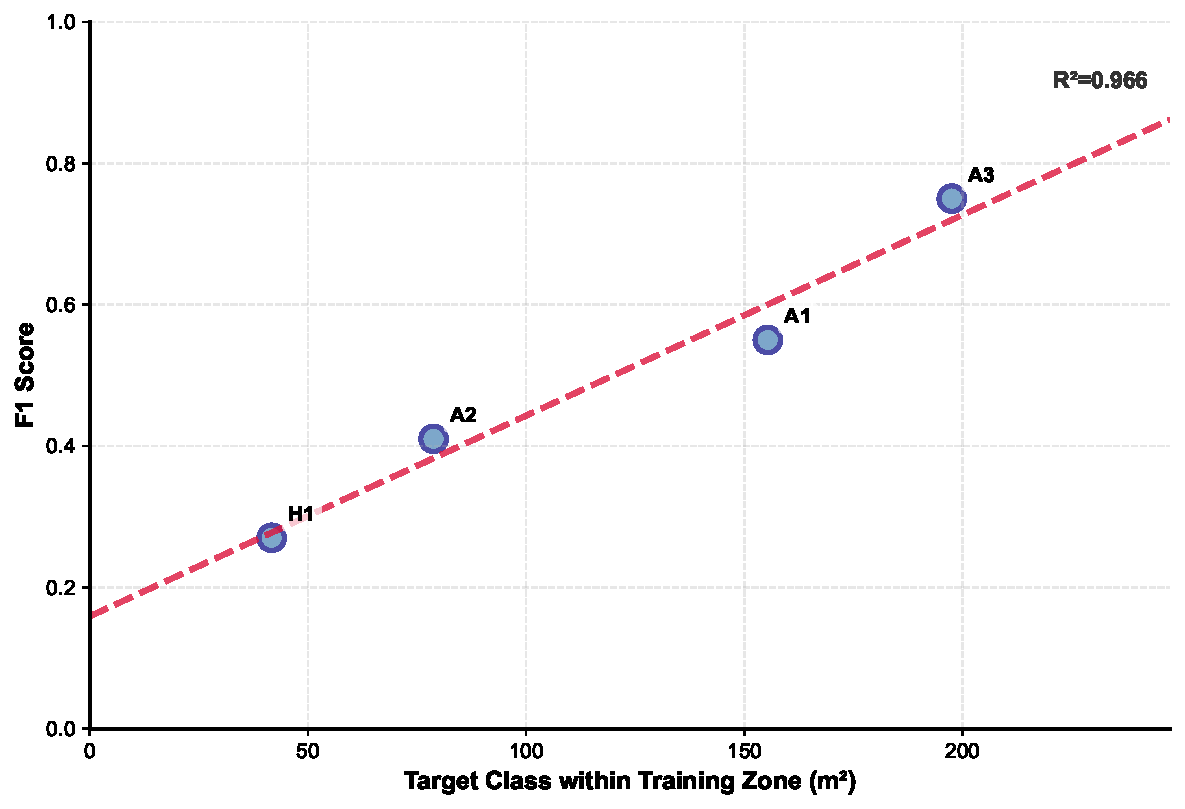
\includegraphics[keepaspectratio]{complete_thesis_files/figure-pdf/cell-3-output-1.pdf}}

\end{minipage}%
%
\begin{minipage}{0.15\linewidth}
~\end{minipage}%

\end{figure}%

}

\caption[Linear regression of annotated training area vs.~F1
score.]{\label{fig-linear_regression}Linear regression of annotated
\hyperref[acronyms_SM]{\emph{S. maire}} area (m\textsuperscript{2})
within the training zone vs.~F1 score trained on RGB imagery
(Table~\ref{tbl-bands}) for each site. Each point represents a site, and
the regression line is shown in red with R\textsuperscript{2}=0.966.}

\end{figure}%

\subsubsection{Hyperparameter
Configuration}\label{hyperparameter-configuration}

To identify which configuration had the greatest impact on detection
accuracy, three key hyperparameters were systematically tested: the loss
function (which guides how the model learns), the
\hyperref[acronyms_LR]{LR} (which controls the magnitude of model weight
adjustments during training), and class weights (which penalise
misclassification of the underrepresented
\hyperref[acronyms_SM]{\emph{S. maire}} class more heavily). This
systematic comparison of hyperparameters (Table~\ref{tbl-hyperparams})
revealed differences in model performance.

\hyperref[acronyms_DICE]{\(L_{Dice}\)} achieved the highest mean
\hyperref[acronyms_F1]{F1} scores (0.56±0.14 for
\hyperref[acronyms_RGB]{RGB} imagery, 0.54±0.25 for MS\(_{rel}\)),
outperforming \hyperref[acronyms_WBCE_D]{\(L_{c}\)} (0.50±0.20 /
0.45±0.26) and \hyperref[acronyms_WBCE]{\(L_{WBCE}\)} (0.48±0.27 /
0.46±0.17). \hyperref[acronyms_LR]{LR} had the most substantial impact
on performance. Models trained with an initial
\hyperref[acronyms_LR]{LR}=0.02 outperformed those with
\hyperref[acronyms_LR]{LR}=5×10\textsuperscript{-5}. When using
\hyperref[acronyms_DICE]{\(L_{Dice}\)} \hyperref[acronyms_F1]{F1} scores
dropped from 0.56±0.14 to 0.13±0.09 (\hyperref[acronyms_RGB]{RGB}) and
from 0.54±0.25 to 0.13±0.11 (MS\(_{rel}\)). The lower
\hyperref[acronyms_LR]{LR} produced random predictions with extremely
high recall (up to 0.98) but negligible precision (0.07--0.14). This
means that virtually any pixel was classified as
\hyperref[acronyms_SM]{\emph{S. maire}} (\quartosfigref{sfig-LR5e-5}).
Class weighting improved \hyperref[acronyms_WBCE_D]{\(L_{c}\)}
performance: \hyperref[acronyms_F1]{F1} gained with each incremental
step adjusting the weights from 1 to 10 to 50 in both
\hyperref[acronyms_RGB]{RGB} and MS\(_{rel}\) (Table~\ref{tbl-weight}).
However, the difference from 10 to 50 is marginal when visually
inspecting results
(\quartosfigref{sfig-predictions_single_weight_comparison}).

\begin{table}

\caption{\label{tbl-hyperparams}Comparison of hyperparameters on
\hyperref[acronyms_SM]{\emph{S. maire}} detection performance
(mean±std), tested on each site separately. Tested hyperparameters
included loss function (\textbf{a}), class weight (\textbf{b}), and
\hyperref[acronyms_LR]{LR} (\textbf{c}).}

\begin{minipage}{\linewidth}

\subcaption{\label{tbl-loss}Results from tested loss functions
(\hyperref[acronyms_WBCE]{\(L_{WBCE}\)},
\hyperref[acronyms_DICE]{\(L_{Dice}\)} (no weight) and
\hyperref[acronyms_WBCE_D]{\(L_{c}\)}) with weight=10 and
\hyperref[acronyms_LR]{LR}=0.02.}

\centering{

\begin{tabular}{llllll}
\toprule
Bands & Loss & F1 & IoU & Precision & Recall\\
\midrule
MS\(_{rel}\) & \hyperref[acronyms_WBCE]{\(L_{WBCE}\)} & 0.46±0.17 & 0.31±0.14 & 0.58±0.22 & 0.56±0.36\\
MS\(_{rel}\) & \hyperref[acronyms_DICE]{\(L_{Dice}\)} & 0.54±0.25 & 0.40±0.23 & 0.65±0.18 & 0.59±0.35\\
MS\(_{rel}\) & \hyperref[acronyms_WBCE_D]{\(L_{c}\)} & 0.45±0.26 & 0.31±0.20 & 0.36±0.14 & 0.69±0.42\\
RGB & \hyperref[acronyms_WBCE]{\(L_{WBCE}\)} & 0.48±0.27 & 0.34±0.23 & 0.55±0.18 & 0.55±0.34\\
RGB & \hyperref[acronyms_DICE]{\(L_{Dice}\)} & 0.56±0.14 & 0.40±0.14 & 0.47±0.13 & 0.76±0.19\\
RGB & \hyperref[acronyms_WBCE_D]{\(L_{c}\)} & 0.50±0.20 & 0.35±0.19 & 0.46±0.21 & 0.56±0.21\\
\bottomrule
\end{tabular}

}

\end{minipage}%
\newline
\begin{minipage}{\linewidth}
~\end{minipage}%
\newline
\begin{minipage}{\linewidth}

\subcaption{\label{tbl-weight}Results from assigning weights 1, 10 and
50 for \hyperref[acronyms_SM]{\emph{S. maire}} class using
\hyperref[acronyms_WBCE_D]{\(L_{c}\)}.}

\centering{

\begin{tabular}{llllll}
\toprule
Bands & Weight & F1 & IoU & Precision & Recall\\
\midrule
MS\(_{rel}\) & 1 & 0.42±0.34 & 0.31±0.29 & 0.55±0.38 & 0.40±0.39\\
MS\(_{rel}\) & 10 & 0.45±0.26 & 0.31±0.20 & 0.36±0.14 & 0.69±0.42\\
MS\(_{rel}\) & 50 & 0.50±0.17 & 0.34±0.14 & 0.42±0.07 & 0.71±0.36\\
RGB & 1 & 0.47±0.17 & 0.32±0.17 & 0.59±0.23 & 0.49±0.28\\
RGB & 10 & 0.50±0.20 & 0.35±0.19 & 0.46±0.21 & 0.56±0.21\\
RGB & 50 & 0.52±0.14 & 0.36±0.12 & 0.49±0.15 & 0.63±0.24\\
\bottomrule
\end{tabular}

}

\end{minipage}%
\newline
\begin{minipage}{\linewidth}
~\end{minipage}%
\newline
\begin{minipage}{\linewidth}

\subcaption{\label{tbl-lr}Results from initial
\hyperref[acronyms_LR]{LRs} (0.02 and 5x10\textsuperscript{-5}) in
combination with a \hyperref[acronyms_LR]{LR}-scheduler with
\hyperref[acronyms_WBCE_D]{\(L_{c}\)} using weight=10.}

\centering{

\begin{tabular}{lllllll}
\toprule
Bands & Loss & LR & F1 & IoU & Precision & Recall\\
\midrule
MS\(_{rel}\) & \hyperref[acronyms_WBCE_D]{\(L_{c}\)} & 5x10\textsuperscript{-5} & 0.14±0.11 & 0.08±0.07 & 0.08±0.07 & 0.98±0.01\\
MS\(_{rel}\) & \hyperref[acronyms_WBCE_D]{\(L_{c}\)} & 0.02 & 0.45±0.26 & 0.31±0.20 & 0.36±0.14 & 0.69±0.42\\
MS\(_{rel}\) & \hyperref[acronyms_DICE]{\(L_{Dice}\)} & 5x10\textsuperscript{-5} & 0.13±0.11 & 0.07±0.06 & 0.07±0.07 & 0.95±0.03\\
MS\(_{rel}\) & \hyperref[acronyms_DICE]{\(L_{Dice}\)} & 0.02 & 0.54±0.25 & 0.40±0.23 & 0.65±0.18 & 0.59±0.35\\
RGB & \hyperref[acronyms_WBCE_D]{\(L_{c}\)} & 5x10\textsuperscript{-5} & 0.19±0.10 & 0.11±0.06 & 0.14±0.08 & 0.44±0.30\\
RGB & \hyperref[acronyms_WBCE_D]{\(L_{c}\)} & 0.02 & 0.50±0.20 & 0.35±0.19 & 0.46±0.21 & 0.56±0.21\\
RGB & \hyperref[acronyms_DICE]{\(L_{Dice}\)} & 5x10\textsuperscript{-5} & 0.13±0.09 & 0.07±0.05 & 0.10±0.08 & 0.23±0.13\\
RGB & \hyperref[acronyms_DICE]{\(L_{Dice}\)} & 0.02 & 0.56±0.14 & 0.40±0.14 & 0.47±0.13 & 0.76±0.19\\
\bottomrule
\end{tabular}

}

\end{minipage}%

\end{table}%

\subsubsection{Band Combinations}\label{band-combinations}

Using base hyperparameters (\hyperref[acronyms_LR]{LR}=0.02, weight=10,
\hyperref[acronyms_WBCE_D]{\(L_{c}\)}), \hyperref[acronyms_RGB]{RGB}
imagery achieved the highest mean \hyperref[acronyms_F1]{F1} score
(0.50) across reserves, though, only marginally better than
MS+IND\(_{rel}\) (mean \hyperref[acronyms_F1]{F1}=0.48). However, this
was not consistent across all sites. At sites A1 and H1,
\hyperref[acronyms_MS]{MS} band combinations outperformed
\hyperref[acronyms_RGB]{RGB} imagery: MS+IND\(_{rel}\) achieved a
notably high \hyperref[acronyms_F1]{F1} of 0.64 on site A1. Performance
varied substantially between the other sites: A3 showed the strongest
and most consistent results across all band types
(\hyperref[acronyms_F1]{F1}=0.60--0.75), whilst site A2 consistently
showed poor performance (\hyperref[acronyms_F1]{F1}=0.08--0.41). Adding
\hyperref[acronyms_RENDVI]{RENDVI} to \hyperref[acronyms_MS]{MS} bands
did not consistently improve performance, except for site A1 where it
contributed to the best result of that site (Table~\ref{tbl-bands}).

\begin{longtable}[]{@{}lllll@{}}

\caption{\label{tbl-bands}F1 scores for tested band combinations
(\hyperref[acronyms_RGB]{RGB}, MS\(_{rel}\), IND\(_{rel}\),
MS+IND\(_{rel}\)) across reserves with \hyperref[acronyms_LR]{LR}=0.02,
weight=10, and \hyperref[acronyms_WBCE_D]{\(L_{c}\)}.}

\tabularnewline

\toprule\noalign{}
Reserve & RGB & MS\(_{rel}\) & IND\(_{rel}\) & MS+IND\(_{rel}\) \\
\midrule\noalign{}
\endhead
\bottomrule\noalign{}
\endlastfoot
A1 & 0.55 & 0.47 & 0.38 & 0.64 \\
A2 & 0.41 & 0.08 & 0.18 & 0.20 \\
A3 & 0.75 & 0.66 & 0.64 & 0.60 \\
H1 & 0.27 & 0.59 & 0.42 & 0.46 \\
\textbf{Mean} & \textbf{0.50} & \textbf{0.45} & \textbf{0.40} &
\textbf{0.48} \\

\end{longtable}

The best-performing model, trained on site A3 with MS\(_{rel}\) bands
and \hyperref[acronyms_DICE]{\(L_{Dice}\)} (weight=1,
\hyperref[acronyms_LR]{LR}=0.02), achieved an \hyperref[acronyms_F1]{F1}
of 0.81 and \hyperref[acronyms_IoU]{IoU} of 0.68
(Table~\ref{tbl-best_single};
\quartostblref{stbl-best_models_single_site_ESK}, S4, S5, S6). Training
metric progression is shown in \quartosfigref{sfig-train_metrics_best}.
Site A3 consistently produced the strongest results, with six of the top
ten models from this reserve. Performance was more variable on other
sites: A1 reached a maximum \hyperref[acronyms_F1]{F1} of 0.65, H1
achieved 0.59, and A2 showed the lowest maximum
\hyperref[acronyms_F1]{F1} of 0.46.

\begin{longtable}[]{@{}
  >{\raggedright\arraybackslash}p{(\linewidth - 16\tabcolsep) * \real{0.1552}}
  >{\raggedright\arraybackslash}p{(\linewidth - 16\tabcolsep) * \real{0.2414}}
  >{\raggedright\arraybackslash}p{(\linewidth - 16\tabcolsep) * \real{0.1034}}
  >{\raggedright\arraybackslash}p{(\linewidth - 16\tabcolsep) * \real{0.0517}}
  >{\raggedright\arraybackslash}p{(\linewidth - 16\tabcolsep) * \real{0.0862}}
  >{\raggedright\arraybackslash}p{(\linewidth - 16\tabcolsep) * \real{0.0862}}
  >{\raggedright\arraybackslash}p{(\linewidth - 16\tabcolsep) * \real{0.0862}}
  >{\raggedright\arraybackslash}p{(\linewidth - 16\tabcolsep) * \real{0.1034}}
  >{\raggedright\arraybackslash}p{(\linewidth - 16\tabcolsep) * \real{0.0862}}@{}}

\caption{\label{tbl-best_single}Top 10 individual single-site models
ranked by F1 score. The top 10 models for each site individually can be
found in Table S2.}

\tabularnewline

\toprule\noalign{}
\begin{minipage}[b]{\linewidth}\raggedright
Reserve
\end{minipage} & \begin{minipage}[b]{\linewidth}\raggedright
Bands
\end{minipage} & \begin{minipage}[b]{\linewidth}\raggedright
Loss
\end{minipage} & \begin{minipage}[b]{\linewidth}\raggedright
W
\end{minipage} & \begin{minipage}[b]{\linewidth}\raggedright
LR
\end{minipage} & \begin{minipage}[b]{\linewidth}\raggedright
F1
\end{minipage} & \begin{minipage}[b]{\linewidth}\raggedright
IoU
\end{minipage} & \begin{minipage}[b]{\linewidth}\raggedright
Prec
\end{minipage} & \begin{minipage}[b]{\linewidth}\raggedright
Rec
\end{minipage} \\
\midrule\noalign{}
\endhead
\bottomrule\noalign{}
\endlastfoot
A3 & MS\(_{rel}\) & \hyperref[acronyms_DICE]{\(L_{Dice}\)} & 1 & 0.02 &
0.81 & 0.68 & 0.74 & 0.88 \\
A3 & MS\(_{rel}\) & \hyperref[acronyms_WBCE_D]{\(L_{c}\)} & 1 & 0.02 &
0.80 & 0.67 & 0.72 & 0.89 \\
A3 & RGB & \hyperref[acronyms_WBCE]{\(L_{WBCE}\)} & 10 & 0.02 & 0.77 &
0.62 & 0.68 & 0.87 \\
A3 & RGB & \hyperref[acronyms_WBCE_D]{\(L_{c}\)} & 10 & 0.02 & 0.75 &
0.60 & 0.74 & 0.76 \\
A3 & RGB & \hyperref[acronyms_DICE]{\(L_{Dice}\)} & 1 & 0.02 & 0.74 &
0.59 & 0.64 & 0.87 \\
A3 & RGB & \hyperref[acronyms_WBCE_D]{\(L_{c}\)} & 1 & 0.02 & 0.72 &
0.57 & 0.62 & 0.86 \\
A3 & MS\(_{rel}\) & \hyperref[acronyms_WBCE_D]{\(L_{c}\)} & 10 & 0.02 &
0.66 & 0.49 & 0.51 & 0.91 \\
A1 & MS\(_{rel}\) & \hyperref[acronyms_WBCE_D]{\(L_{c}\)} & 50 & 0.02 &
0.65 & 0.48 & 0.52 & 0.87 \\
A3 & RGB & \hyperref[acronyms_WBCE_D]{\(L_{c}\)} & 50 & 0.02 & 0.65 &
0.48 & 0.52 & 0.86 \\
A1 & MS+IND\(_{rel}\) & \hyperref[acronyms_WBCE_D]{\(L_{c}\)} & 10 &
0.02 & 0.64 & 0.47 & 0.51 & 0.87 \\

\end{longtable}

Visual inspection of the predictions reveals clear differences in model
behaviour (Figure~\ref{fig-predictions_single}). Site A3 predictions
show high correspondence with ground truth, especially for
\hyperref[acronyms_DICE]{\(L_{Dice}\)}, which yielded cleaner edges,
whereas \hyperref[acronyms_WBCE_D]{\(L_{c}\)} models produced frayed
edges and additional noise. Site A2 predictions were consistently
smaller than ground-truthed area. Site H1 showed the poorest
performance, with consistent misclassified patches and additional noise.
\hyperref[acronyms_WBCE_D]{\(L_{c}\)} with higher weights introduced
more noise in both \hyperref[acronyms_RGB]{RGB} and
\hyperref[acronyms_MS]{MS} imagery predictions compared to
\hyperref[acronyms_DICE]{\(L_{Dice}\)}.

\begin{figure}

\centering{

\pandocbounded{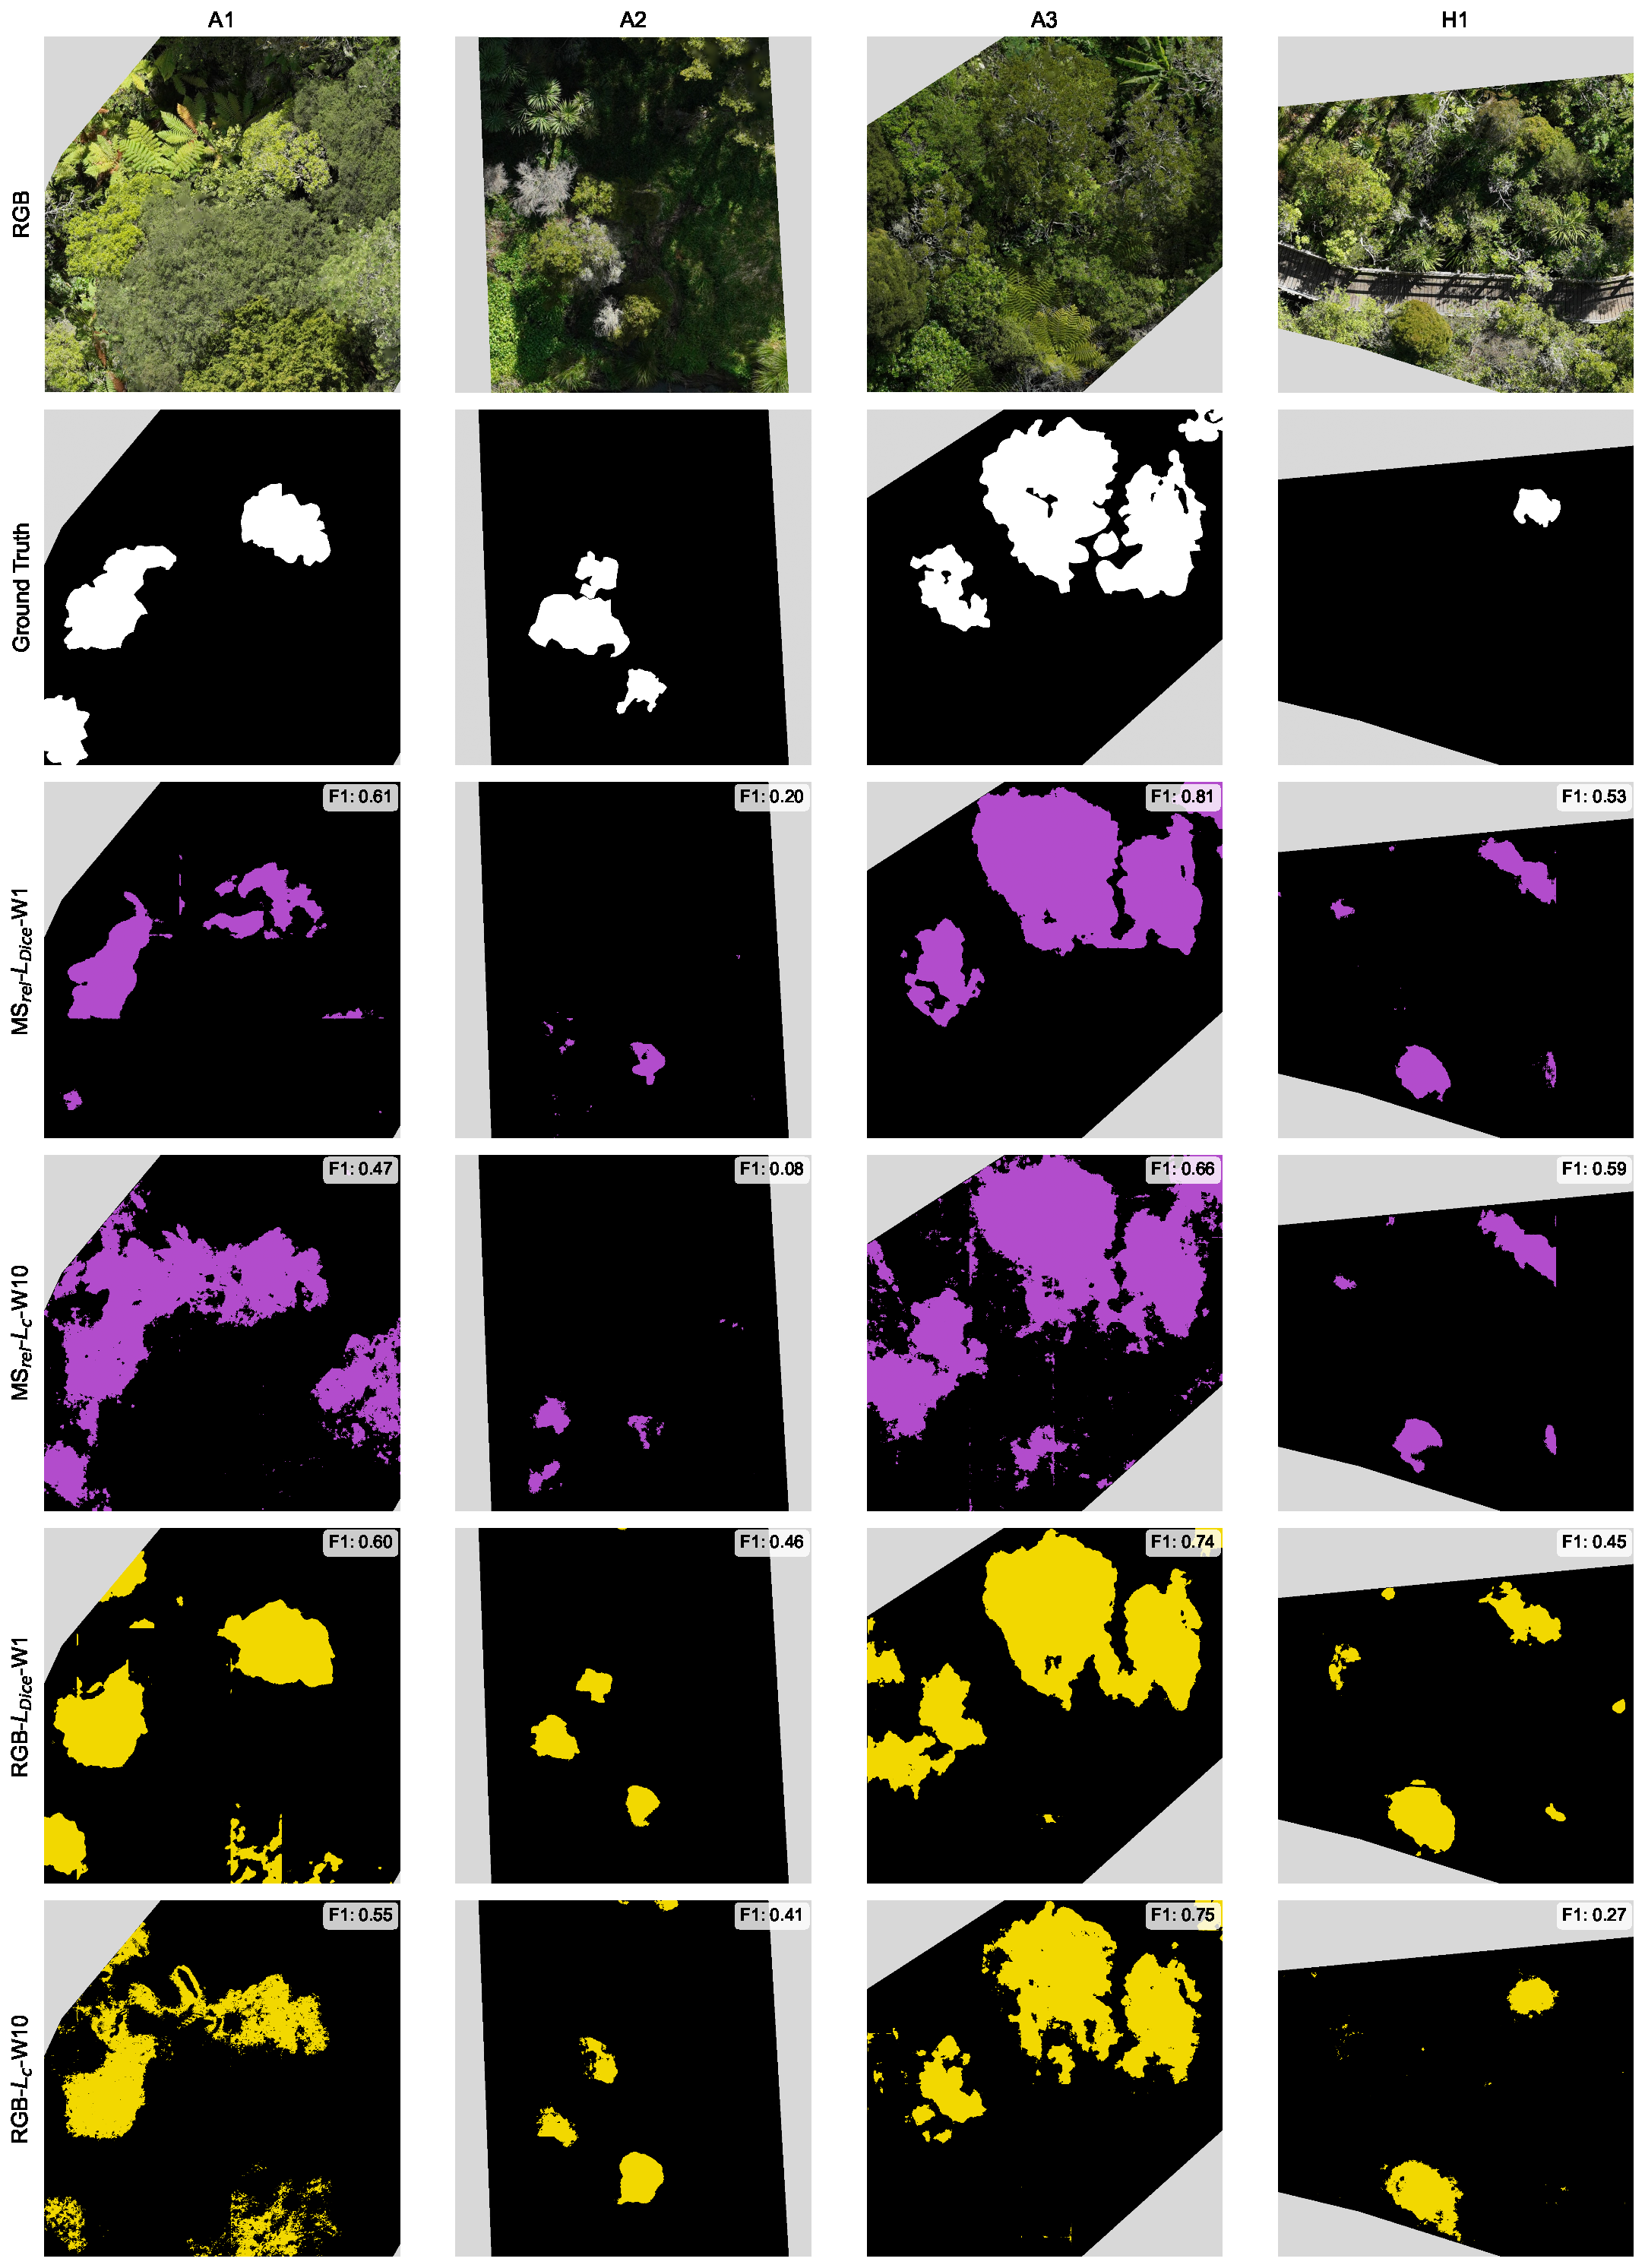
\includegraphics[keepaspectratio]{complete_thesis_files/figure-pdf/fig-predictions_single-output-1.pdf}}

}

\caption[Predictions
single-site.]{\label{fig-predictions_single}Predictions from the
best-performing single-site models for the test zone for each reserve
for a 15x15 m extent. Pink overlays indicate predictions on
\hyperref[acronyms_MS]{MS} imagery, yellow overlays on
\hyperref[acronyms_RGB]{RGB} imagery. Model configurations are listed on
the left; all were trained with a \hyperref[acronyms_LR]{LR} of 0.02.
For example RGB-\(L_{c}\)-W10 reads as: ``model trained on RGB bands
using \hyperref[acronyms_WBCE_D]{\(L_{c}\)} with a weight of 10''.}

\end{figure}%

\subsection{Multi-site}\label{multi-site}

\subsubsection{Band and Loss Functions}\label{band-and-loss-functions}

\hyperref[acronyms_RGB]{RGB} bands outperformed
\hyperref[acronyms_MS]{MS} bands in the multi-site setting, with the
three best models all using \hyperref[acronyms_RGB]{RGB} imagery
(Table~\ref{tbl-multi_site}). This trend confirms the single-site
results, however, the performance gap between
\hyperref[acronyms_RGB]{RGB} and \hyperref[acronyms_MS]{MS} imagery is
much more pronounced with \hyperref[acronyms_F1]{F1}=0.51
(\hyperref[acronyms_RGB]{RGB}) and \hyperref[acronyms_F1]{F1}=0.35
(\hyperref[acronyms_MS]{MS}).

\begin{longtable}[]{@{}
  >{\raggedright\arraybackslash}p{(\linewidth - 12\tabcolsep) * \real{0.2708}}
  >{\raggedright\arraybackslash}p{(\linewidth - 12\tabcolsep) * \real{0.1250}}
  >{\raggedright\arraybackslash}p{(\linewidth - 12\tabcolsep) * \real{0.1667}}
  >{\raggedright\arraybackslash}p{(\linewidth - 12\tabcolsep) * \real{0.1042}}
  >{\raggedright\arraybackslash}p{(\linewidth - 12\tabcolsep) * \real{0.1042}}
  >{\raggedright\arraybackslash}p{(\linewidth - 12\tabcolsep) * \real{0.1250}}
  >{\raggedright\arraybackslash}p{(\linewidth - 12\tabcolsep) * \real{0.1042}}@{}}

\caption{\label{tbl-multi_site}The performance metrics from the 10 best
performing model configurations trained on the multi-site dataset,
sorted by F1 score. A table with all models is available in
\quartostblref{stbl-multi_site_all}.}

\tabularnewline

\toprule\noalign{}
\begin{minipage}[b]{\linewidth}\raggedright
Bands
\end{minipage} & \begin{minipage}[b]{\linewidth}\raggedright
Loss
\end{minipage} & \begin{minipage}[b]{\linewidth}\raggedright
Weight
\end{minipage} & \begin{minipage}[b]{\linewidth}\raggedright
F1
\end{minipage} & \begin{minipage}[b]{\linewidth}\raggedright
IoU
\end{minipage} & \begin{minipage}[b]{\linewidth}\raggedright
Prec
\end{minipage} & \begin{minipage}[b]{\linewidth}\raggedright
Rec
\end{minipage} \\
\midrule\noalign{}
\endhead
\bottomrule\noalign{}
\endlastfoot
RGB & \hyperref[acronyms_WBCE_D]{\(L_{c}\)} & 50 & 0.51 & 0.34 & 0.39 &
0.72 \\
RGB & \hyperref[acronyms_DICE]{\(L_{Dice}\)} & 1 & 0.50 & 0.33 & 0.45 &
0.56 \\
RGB & \hyperref[acronyms_WBCE_D]{\(L_{c}\)} & 10 & 0.45 & 0.29 & 0.31 &
0.81 \\
MS\(_{rel}\) & \hyperref[acronyms_WBCE_D]{\(L_{c}\)} & 50 & 0.35 & 0.22
& 0.23 & 0.75 \\
MS\(_{rel}\) & \hyperref[acronyms_WBCE_D]{\(L_{c}\)} & 10 & 0.30 & 0.18
& 0.27 & 0.34 \\
IND\(_{abs}\) & \hyperref[acronyms_WBCE_D]{\(L_{c}\)} & 10 & 0.22 & 0.12
& 0.23 & 0.20 \\
IND\(_{abs}\) & \hyperref[acronyms_WBCE_D]{\(L_{c}\)} & 50 & 0.19 & 0.10
& 0.12 & 0.52 \\
MS\(_{rel}\) & \hyperref[acronyms_DICE]{\(L_{Dice}\)} & 1 & 0.16 & 0.09
& 0.44 & 0.10 \\
MS\(_{abs}\) & \hyperref[acronyms_WBCE_D]{\(L_{c}\)} & 50 & 0.16 & 0.09
& 0.17 & 0.15 \\
MS+IND\(_{abs}\) & \hyperref[acronyms_DICE]{\(L_{Dice}\)} & 1 & 0.16 &
0.09 & 0.11 & 0.31 \\

\end{longtable}

Absolute-calibrated band combinations (MS\(_{abs}\), IND\(_{abs}\),
MS+IND\(_{abs}\)) showed poor generalisation in multi-site training,
with \hyperref[acronyms_F1]{F1} scores ≤0.22 and subsequently also poor
visual results (Figure~\ref{fig-predictions-multisite}).
\hyperref[acronyms_DICE]{\(L_{Dice}\)} on \hyperref[acronyms_MS]{MS}
imagery showed low noise but exhibited substantial under-segmentation
and misclassification, where both sites A1
(\hyperref[acronyms_F1]{F1}=0.00) and A3
(\hyperref[acronyms_F1]{F1}=0.07) were subject to these issues. This was
also visible in training metrics progression, where
\hyperref[acronyms_IoU]{IoU} plateaued after \textasciitilde30 epochs
(\quartosfigref{sfig-train_metrics_multi_site}).

\subsubsection{Best-performing Multi-site
Models}\label{best-performing-multi-site-models}

Despite systematic optimisation, multi-site models achieved
substantially lower performance than single-site models. The best
multi-site configuration (\hyperref[acronyms_RGB]{RGB} imagery,
\hyperref[acronyms_WBCE_D]{\(L_{c}\)}, weight=50) achieved an
\hyperref[acronyms_F1]{F1} of 0.51 and \hyperref[acronyms_IoU]{IoU} of
0.34, representing a 37\% reduction in \hyperref[acronyms_F1]{F1}
compared to the best single-site model. Only the
\hyperref[acronyms_RGB]{RGB} imagery model with
\hyperref[acronyms_WBCE_D]{\(L_{c}\)} achieved performance comparable to
some single-site models (\hyperref[acronyms_F1]{F1}=0.54). Across all
configurations, multi-site predictions were notably noisier than their
single-site counterparts (Figure~\ref{fig-predictions-multisite}),
indicating that the model struggled to learn consistent
\hyperref[acronyms_SM]{\emph{S. maire}} characteristics across different
forest structures and lighting conditions. Notably, visually one of the
best results was on a site (A2) that showed poor results in the
single-site setting, identifying \hyperref[acronyms_SM]{\emph{S. maire}}
accurately (RGB, \(L_{c}\), weight=50; \hyperref[acronyms_F1]{F1}=0.54;
Figure~\ref{fig-predictions-multisite}).

\begin{figure}[H]

\centering{

\pandocbounded{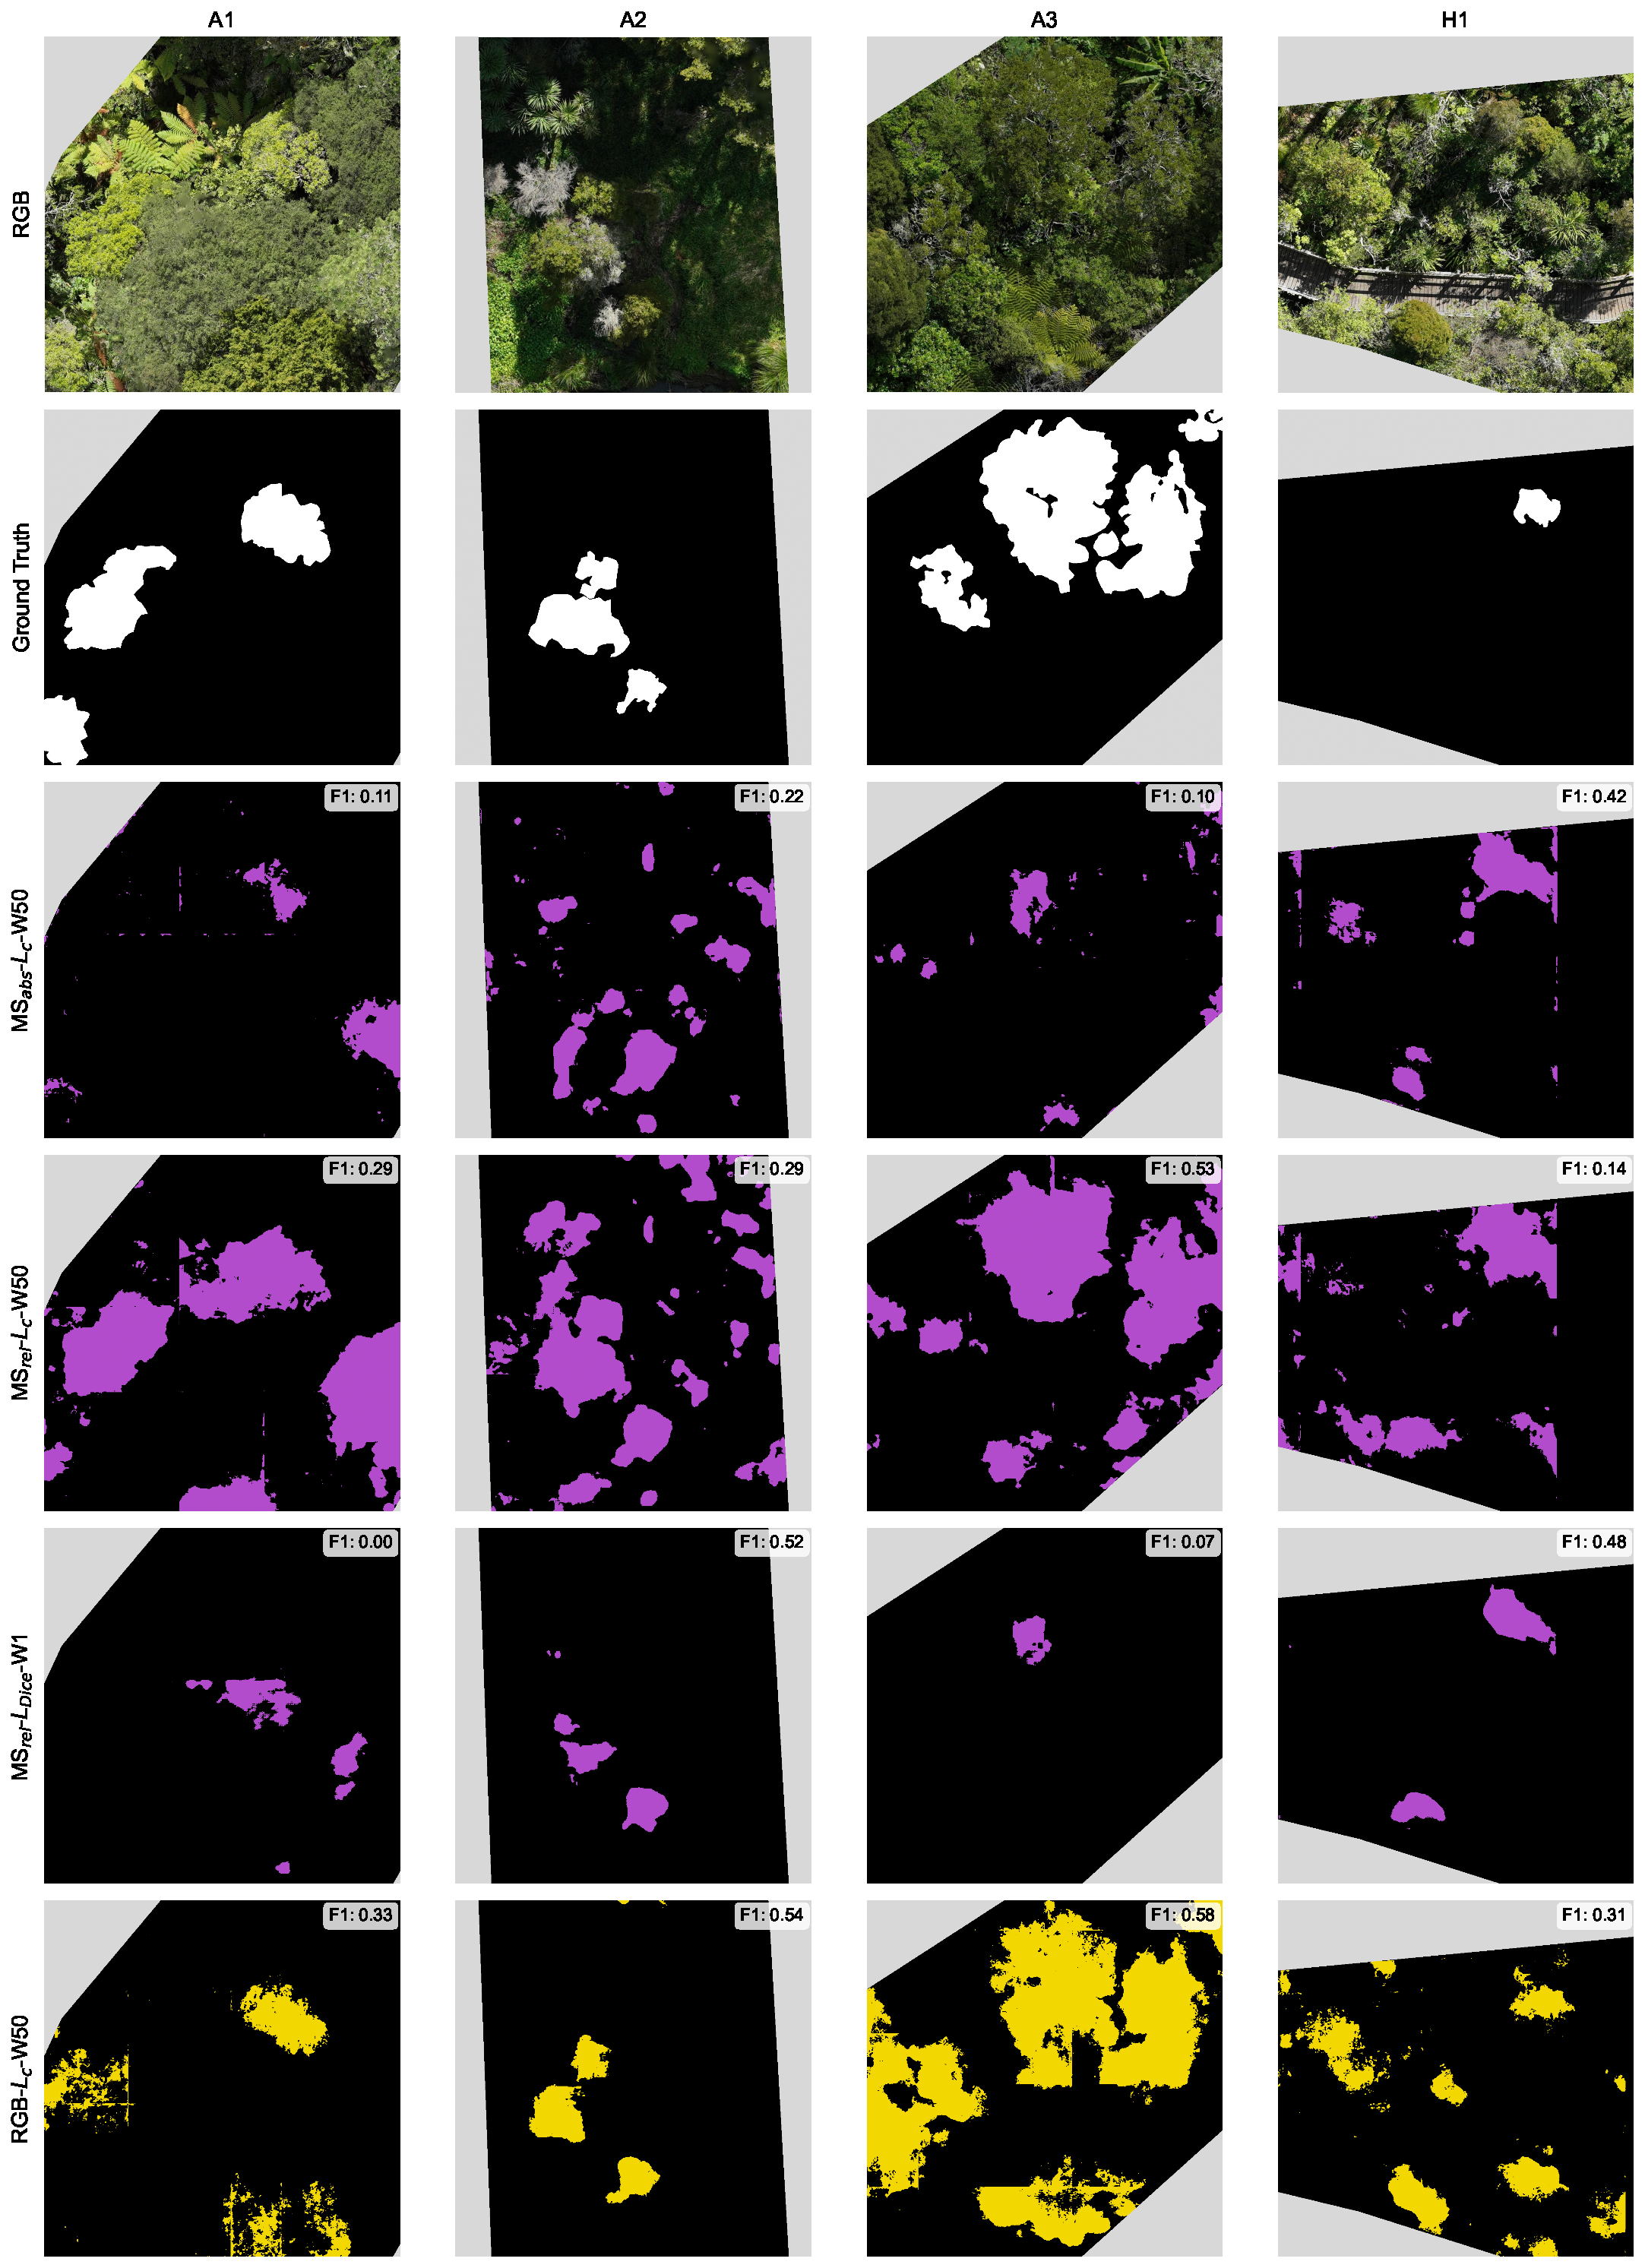
\includegraphics[keepaspectratio]{complete_thesis_files/figure-pdf/fig-predictions-multisite-output-1.pdf}}

}

\caption[Predictions
multi-site.]{\label{fig-predictions-multisite}Predictions from the
best-performing multi-site models for the test zone for each reserve for
a 15x15 m extent. Pink overlays indicate predictions on
\hyperref[acronyms_MS]{MS} imagery, yellow overlays on
\hyperref[acronyms_RGB]{RGB} imagery. Model configurations are listed on
the left; all models were trained with a \hyperref[acronyms_LR]{LR} of
0.02. For example RGB-\(L_{c}\)-W50 reads as: ``model trained on RGB
bands using \hyperref[acronyms_WBCE_D]{\(L_{c}\)} with a weight of
50''.}

\end{figure}%

\section{LiDAR Tree Segmentation}\label{lidar-tree-segmentation-1}

Two instance segmentation algorithms (TreeLearn and Treeiso) were tested
to isolate individual tree point clouds from the forest point cloud.
However, qualitative assessment of the two trialled segmentation methods
revealed significant challenges with both approaches.

TreeLearn did not successfully segment individual trees and produced
messy, near random looking segmentations
(Figure~\ref{fig-tree_instance_seg} a-c). Treeiso performed better,
producing recognisable tree segments, but segmentations frequently
included portions of adjacent tree crowns, limiting their quality for
species-specific classification (Figure~\ref{fig-tree_instance_seg}
d-f). Given these limitations and the more promising results from
\hyperref[acronyms_MS]{MS} imagery analysis, further development of
\hyperref[acronyms_LiDAR]{LiDAR}-based segmentation was not pursued
within the timeframe of this thesis.

\begin{figure}

\centering{

\begin{figure}[H]

\begin{minipage}{0.33\linewidth}

\centering{

\pandocbounded{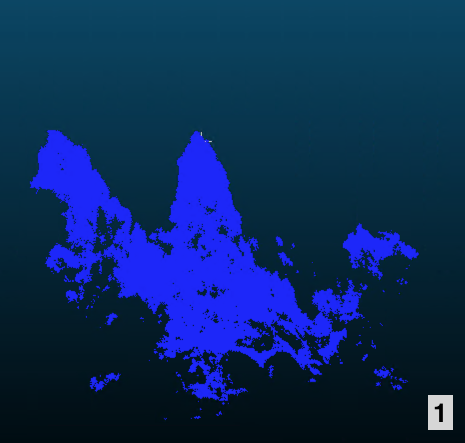
\includegraphics[keepaspectratio]{../2_1_figures/tree_instance_seg/TreeLearn.png}}

}

\subcaption{\label{fig-a}Segmented points of segmentation 1 using
TreeLearn.}

\end{minipage}%
%
\begin{minipage}{0.01\linewidth}
~\end{minipage}%
%
\begin{minipage}{0.33\linewidth}

\centering{

\pandocbounded{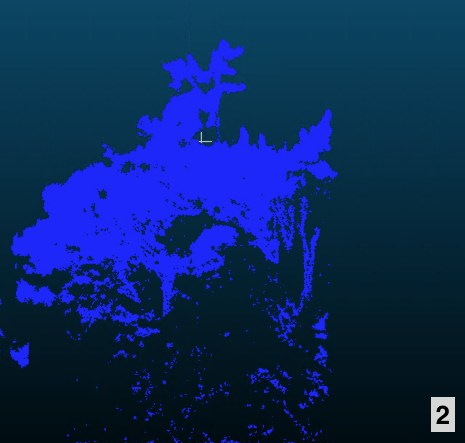
\includegraphics[keepaspectratio]{../2_1_figures/tree_instance_seg/TreeLearn2.png}}

}

\subcaption{\label{fig-b}Segmented points of segmentation 2 using
TreeLearn.}

\end{minipage}%
%
\begin{minipage}{0.01\linewidth}
~\end{minipage}%
%
\begin{minipage}{0.33\linewidth}

\centering{

\pandocbounded{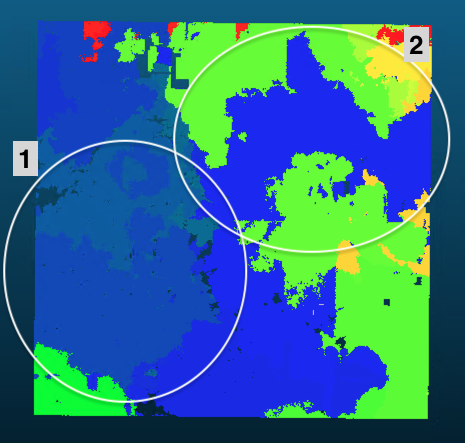
\includegraphics[keepaspectratio]{../2_1_figures/tree_instance_seg/TreeLearnTop.png}}

}

\subcaption{\label{fig-c}TreeLearn segmentation map in top-down nadir
view.}

\end{minipage}%
\newline
\begin{minipage}{0.33\linewidth}

\centering{

\pandocbounded{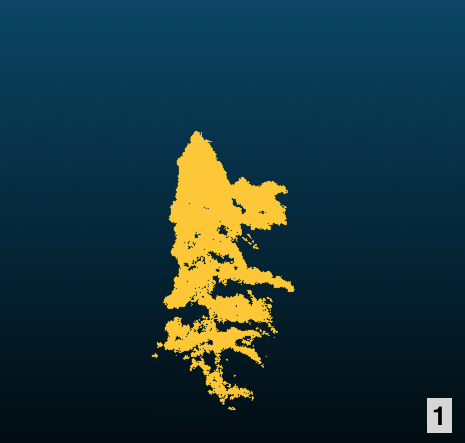
\includegraphics[keepaspectratio]{../2_1_figures/tree_instance_seg/TreeIso.png}}

}

\subcaption{\label{fig-d}Segmented points of segmentation 1 using
Treeiso.}

\end{minipage}%
%
\begin{minipage}{0.01\linewidth}
~\end{minipage}%
%
\begin{minipage}{0.33\linewidth}

\centering{

\pandocbounded{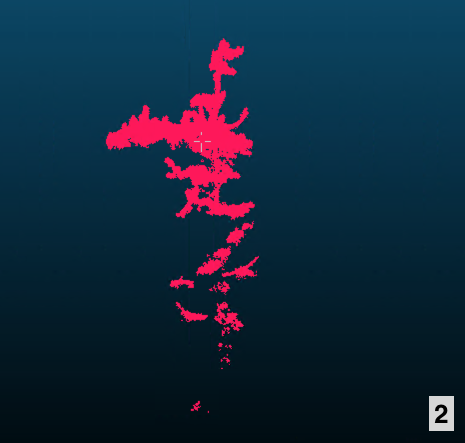
\includegraphics[keepaspectratio]{../2_1_figures/tree_instance_seg/TreeIso2.png}}

}

\subcaption{\label{fig-e}Segmented points of segmentation 2 using
Treeiso.}

\end{minipage}%
%
\begin{minipage}{0.01\linewidth}
~\end{minipage}%
%
\begin{minipage}{0.33\linewidth}

\centering{

\pandocbounded{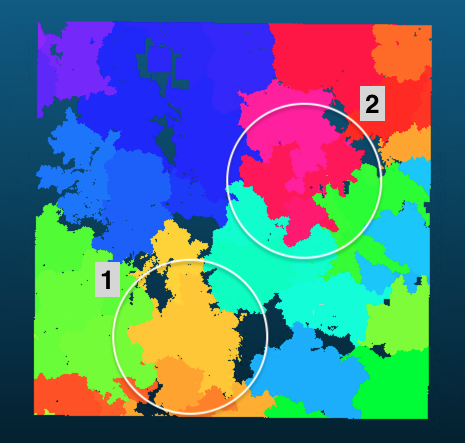
\includegraphics[keepaspectratio]{../2_1_figures/tree_instance_seg/TreeIsoTop.png}}

}

\subcaption{\label{fig-f}Treeiso segmentation map in top-down nadir
view.}

\end{minipage}%

\end{figure}%

}

\caption[TreeLearn vs.~Treeiso.]{\label{fig-tree_instance_seg}Comparison
between extracted segmentation groups using TreeLearn
(\textbf{a}--\textbf{c}) and Treeiso (\textbf{d}--\textbf{f}).}

\end{figure}%

\newpage{}

\chapter{Chapter 4 Discussion}\label{discussion}

\hyperref[acronyms_AP]{\emph{A. psidii}} (which causes
\hyperref[acronyms_MR]{myrtle rust}) has spread globally over the past
two decades with dramatic consequences for Myrtaceae, in severe cases
even leading to local extinctions
(\citeproc{ref-fenshamImminentExtinction2020}{Fensham et al., 2020};
\citeproc{ref-fenshamUnprecedentedextinction2021}{Fensham \&
Radford-Smith, 2021}). Since the pathogen's arrival in 2017 in Aotearoa,
concerns have emerged for native Myrtaceae
(\citeproc{ref-joEcologicalimportance2022}{Jo et al., 2022};
\citeproc{ref-sutherlandMonitoringAustropuccinia2020}{Sutherland et al.,
2020}; \citeproc{ref-toome-hellerChasingmyrtle2020}{Toome-Heller et al.,
2020}). Accurate mapping, especially of highly susceptible species like
\hyperref[acronyms_SM]{\emph{S. maire}}, is critical for conservation
efforts. However, the rarity of \hyperref[acronyms_SM]{\emph{S. maire}}
can be one of the main limiting factors in research topics evolving
around this species
(\citeproc{ref-mccarthyFunctionalAssessment2024}{McCarthy et al.,
2024}). Advances in \hyperref[acronyms_UAV]{UAV} technology and
\hyperref[acronyms_DL]{deep learning} architectures have enabled forest
inventory monitoring globally
(\citeproc{ref-abreu-diasAdvancesAutomated2025}{Abreu-Dias et al.,
2025}; \citeproc{ref-oscoreviewdeep2021}{Osco et al., 2021};
\citeproc{ref-wolkReviewSemantic2024}{Wołk \& Tatara, 2024}). This
thesis applied these technologies in a case study to map
\hyperref[acronyms_SM]{\emph{S. maire}}, a rare native tree threatened
by \hyperref[acronyms_MR]{myrtle rust}, in dense and complex native
forests based on high-resolution \hyperref[acronyms_UAV]{UAV} imagery
and \hyperref[acronyms_LiDAR]{LiDAR} point clouds.

Detection of \hyperref[acronyms_SM]{\emph{S. maire}} was attempted using
a 2D \hyperref[acronyms_DL]{deep learning} approach with U-Net semantic
segmentation. Model performance varied significantly from site to site
(\hyperref[acronyms_F1]{F1} ranging from 0.46--0.81), and results did
not transfer well to multi-site detection (best
\hyperref[acronyms_F1]{F1}=0.51). Regarding spectral and hyperparameter
configurations, \hyperref[acronyms_RGB]{RGB} imagery at higher spatial
resolution (1.5 cm) produced marginally better results
(\hyperref[acronyms_F1]{F1}=0.50) than lower resolution
\hyperref[acronyms_MS]{MS} imagery (2.5 cm; mean
\hyperref[acronyms_F1]{F1}=0.45--0.48). Hyperparameters configuration
had substantial impact on model performance:
\hyperref[acronyms_DICE]{\(L_{Dice}\)} and a \hyperref[acronyms_LR]{LR}
of 0.02 in combination with adaptive scheduling generally led to best
results. For the point cloud approach, the TreeLearn algorithm was
unsuccessful, whilst the Treeiso segmentation method produced
recognisable tree segments and showed promise for improving the
\hyperref[acronyms_DL]{deep learning}-based
\hyperref[acronyms_SM]{\emph{S. maire}} detection workflow
(Figure~\ref{fig-tree_instance_seg}). These findings indicate that
\hyperref[acronyms_UAV]{UAV}-based \hyperref[acronyms_DL]{deep learning}
methods can detect \hyperref[acronyms_SM]{\emph{S. maire}} at individual
sites under optimal conditions, but additional research, particularly in
acquiring training data and addressing radiometric calibration issues,
is necessary before such an approach can be reliably applied for
conservation purposes.

Supporting this conclusion, analysis of the relationship between
training data area and detection performance
(Figure~\ref{fig-linear_regression}) demonstrates a strong positive
trend: a Pearson correlation test showed a significant linear
relationship between available \hyperref[acronyms_SM]{\emph{S. maire}}
annotation area and F1 scores (p = 0.017, n = 4), with linear regression
explaining 96.6\% of the variance in performance across sites (R² =
0.966). While the sample size of n = 4 was too small to meet
conventional statistical robustness thresholds, the consistency of this
trend across sites is strong evidence that acquisition of additional
training data would substantially improve detection capabilities. Future
research expanding to additional \hyperref[acronyms_SM]{\emph{S. maire}}
populations should therefore directly address this identified
bottleneck, enabling the development of more generalisable detection
models suitable for operational conservation applications.

In the following sections, data availability and collection, and
processing constraints are discussed in detail, followed by the
methodological approach and hyperparameter configurations, spectral
considerations, and challenges for model generalisation across sites.
Comparison of performance to other studies embeds the results within
existing literature, whilst broader implications for species monitoring
and conservation are explored. Limitations and recommendations for
future research are discussed throughout these sections.

\section{Data Collection and
Processing}\label{data-collection-and-processing}

\subsection{Temporal Considerations}\label{temporal-considerations}

Initial data collection was planned for April, but due to weather
constraints and temporal limitations of this thesis, the
\hyperref[acronyms_MS]{MS} imagery was collected in September. April was
originally chosen because the maximum symptom occurrence for MR is
between March and April
(\citeproc{ref-beresfordImpactsmyrtle2019}{Beresford et al., 2019}), but
had to be redone because of uncontinuous lighting conditions leading to
artefacts in the generated orthomosaic
(\quartosfigref{sfig-ms_seamline}). While the scope of this thesis did
not investigate disease detection directly, it is likely that this would
be more successful if data were collected between March and April as
intended.

Outside of disease detection, the peak growing season for
\hyperref[acronyms_SM]{\emph{S. maire}} is between December and
February. This is when flowering rates are highest. This means data
collection at this time could enhance detection performance through more
distinctive spectral signatures of new growth tissue or phenological
traits. However, since flowering is limited (e.g.~tree is not fully
covered in flowers) and berries are small, leveraging these phenological
traits would be challenging at practical flight heights. Furthermore,
Robbins et al. (\citeproc{ref-robbinsNatureScanRGB2025}{2025}) observed
that data collection at higher latitudes requires timing closer to
summer solstice for optimal results due to lower sun angles and reduced
vegetation activity. Future investigations into species detection should
therefore prioritise data acquisition during peak growing season
(December--February) to maximise spectral differentiation between
species.

\subsection{Sensor and Processing Constraints}\label{sec-calibration}

The DJI \hyperref[acronyms_M3M]{M3M} is a relatively low-cost
\hyperref[acronyms_MS]{MS} \hyperref[acronyms_UAV]{UAV} platform that is
promoted as a practical option for aerial surveying, crop growth
monitoring and natural resource surveys (\citeproc{ref-djiMavic3}{DJI,
n.d.-d}). The sensor collects \hyperref[acronyms_RGB]{RGB} imagery plus
four \hyperref[acronyms_MS]{MS} bands (\hyperref[acronyms_G]{G},
\hyperref[acronyms_R]{R}, \hyperref[acronyms_RE]{RE}, and
\hyperref[acronyms_NIR]{NIR}), bands that have proven useful for
vegetation mapping and species detection in \hyperref[acronyms_DL]{deep
learning} studies using other platforms and sensors
(\citeproc{ref-barretoDataAugmentation2023}{Barreto et al., 2023};
\citeproc{ref-ulkuDeepSemantic2022}{Ulku et al., 2022};
\citeproc{ref-zhangIrUNetIrregular2021}{T. Zhang et al., 2021}).
However, especially in \hyperref[acronyms_MR]{myrtle rust} mapping, the
blue band and indices derived from it, have been identified as an
important factor to identify the disease
(\citeproc{ref-heimMultispectralAerial2019}{Heim et al., 2019}).
Nonetheless, the low cost and ease of use renders it a viable option for
the detection of rare and threatened species, particularly when budgets
are as limited as it is the case for conservation efforts of species
like \hyperref[acronyms_SM]{\emph{S. maire}}, that are often managed by
budget-constrained community restoration groups.

Accurate radiometric calibration of \hyperref[acronyms_MS]{MS} imagery
is essential for cross-site comparability
(\citeproc{ref-olssonRadiometricCorrection2021}{Olsson et al., 2021};
\citeproc{ref-swaminathanSelectionappropriate2024}{Swaminathan et al.,
2024}). This thesis faced several limitations regarding these
calibrations. Firstly, Agisoft Metashape does not officially support the
DJI \hyperref[acronyms_M3M]{M3M} for reflectance calibration, although
it supports the identical DJI Phantom 4 \hyperref[acronyms_MS]{MS}
\hyperref[acronyms_UAV]{UAV} calibration workflow
(\citeproc{ref-agisoftllcAgisoftMetashape2025}{Agisoft LLC, 2025}).
Furthermore, \hyperref[acronyms_CRP]{CRP} saturation in
\hyperref[acronyms_R]{R} and \hyperref[acronyms_G]{G} bands
(\quartosfigref{sfig-crp_hist}) compromised absolute calibration and
thus likely contributing to poor multi-site generalisation.

Best practices to mitigate calibration issues include thermal
stabilisation of the sensor prior to data collection,
\hyperref[acronyms_CRP]{CRP} capture at mission altitude, larger panels
for adequate pixel coverage, and usage of multiple
\hyperref[acronyms_CRP]{CRPs} with different reflectances below 20\% to
prevent saturation
(\citeproc{ref-olssonRadiometricCorrection2021}{Olsson et al., 2021}).
The \hyperref[acronyms_M3M]{M3M} used in this thesis permitted only
automatic exposure, resulting in variable exposure settings for
individual images (\quartosfigref{sfig-exposure}), i.e., preventing the
use of consistent gain and shutter speed recommended for reproducible
results (\citeproc{ref-swaminathanSelectionappropriate2024}{Swaminathan
et al., 2024}). The \hyperref[acronyms_M3M]{M3M}'s absence from
\hyperref[acronyms_DL]{deep learning} species detection literature
(\citeproc{ref-abreu-diasAdvancesAutomated2025}{Abreu-Dias et al.,
2025}) likely reflects these calibration challenges in non-research
grade \hyperref[acronyms_UAV]{UAVs}.

For multi-site generalisation, the model trained on relatively
calibrated \hyperref[acronyms_MS]{MS} images was presumably limited by
not correcting for different exposure factors, whereas absolute
calibration failed due to \hyperref[acronyms_CRP]{CRP} saturation from
overexposed images (\quartosfigref{sfig-crp_hist}). Therefore, future
research should carefully select \hyperref[acronyms_MS]{MS} imaging
sensors and prioritise those with official software support. Calibration
panels should be selected to avoid saturation issues, and the best
practices for radiometric calibration mentioned above should be followed
where possible. Additionally, normalisation techniques such as histogram
stretching (0.01--99.9\%) applied to \hyperref[acronyms_RGB]{RGB}
imagery by Schiefer et al.
(\citeproc{ref-schieferMappingforest2020}{2020}) may improve cross-site
generalisation.

Finally, artefacts in both the processed \hyperref[acronyms_RGB]{RGB}
and \hyperref[acronyms_MS]{MS} orthomosaics were observed, presumably
caused by wind-induced canopy movement between the capture of subsequent
images (\quartosfigref{sfig-artefacts}). These artefacts were not
present in the raw images, indicating they were introduced during the
orthomosaic generation process. Such artefacts distort canopy features
and can therefore negatively impact model performance due to
misrepresentation. Future research should therefore consider adopting a
methodology in which training is based on raw images rather than
orthomosaics, to avoid such artefacts and thus improve model
performance. This approach has been applied previously for species
detection in environmental monitoring
(\citeproc{ref-jamesDetectingplant2020}{James \& Bradshaw, 2020}).
However, the annotation workflow would be considerably more
time-consuming than working with orthomosaics. Additionally, such an
approach would require more complex post-processing to georeference
detection results correctly. A notable advantage lies in the expanded
training dataset, where multiple images of the same tree from different
viewing angles could be taken. Therefore, as long as provided
orthomosaic software cannot overcome these artefacts in high-resolution
imagery, training on raw images may offer better detection performance
at the cost of complicated results processing.

\subsection{Reference Data
Considerations}\label{reference-data-considerations}

Site reconnaissance relied on iNaturalist records and local expert
knowledge to identify candidate \hyperref[acronyms_SM]{\emph{S. maire}}
populations. Local experts were consulted and a selection of the most
promising sites between Auckland, Hamilton and Tauranga was checked,
with only four sites deemed suitable (Section~\ref{sec-research_sites}).
Therefore, acquiring a larger dataset was not possible, which is a
challenge that may also persist in a large-scale study, due to the
rareness of the species. Thus, the most prominent issue for a future
study lies in identifying and accessing more sites with larger
\hyperref[acronyms_SM]{\emph{S. maire}} populations. However, finding
substantially larger populations may prove challenging given the rarity
and scattered distribution of \hyperref[acronyms_SM]{\emph{S. maire}},
and if population numbers on other sites prove equally limited, the
logistical burden of conducting \hyperref[acronyms_UAV]{UAV} surveys
across numerous sites may become impractical to manage alongside other
conservation priorities.

Whilst iNaturalist observations were valuable for identifying
populations, their spatial precision was unsuitable for direct use for
annotating, and the records were incomplete. Collecting reliable
reference data required comprehensive field verification across sites.
Ground-truthing then provided \hyperref[acronyms_GNSS]{GNSS} positions
of individual trees. Although manual annotation is usually a bottleneck,
it was manageable given the limited dataset size. However, if a scaled
approach were attempted, this might become a challenge. Annotations were
generated through manual digitisation of \hyperref[acronyms_SM]{\emph{S.
maire}} canopy from orthomosaics guided by these field-collected
positions. Spatial offsets between \hyperref[acronyms_RGB]{RGB} and
\hyperref[acronyms_MS]{MS} orthomosaics required separate annotation of
each orthomosaic. This introduced additional complexity and prevented
the creation of a combined dataset. The accuracy and confidence in these
annotations would be improved with the inclusion of additional people to
validate the reference data
(\citeproc{ref-kattenbornConvolutionalNeural2019}{Kattenborn et al.,
2019}).

\subsection{Site Limitations}\label{site-limitations}

Time and resource constraints meant this thesis was restricted to four
research sites. This limited development of models generalising across
the diverse conditions where \hyperref[acronyms_SM]{\emph{S. maire}}
occurs. Site-specific characteristics substantially affected
performance. For example: sites A1 and A3 were expected to yield similar
results given proximity and comparable dataset size, yet A3 outperformed
A1. This suggests that site-specific variations like vegetation
composition or foliage health may have impacted results. It is assumed
that lower performance at sites A2 and H1 can be traced to extremely
limited training data (6--9 images compared to 21--26 at
better-performing sites), or potentially a false annotation at site H1,
which was consistently predicted as \hyperref[acronyms_SM]{\emph{S.
maire}}. Even with multi-site training, generalisation proved
problematic. Therefore, a more extensive study should also consider
including sites containing \hyperref[acronyms_SM]{\emph{S. maire}}
populations within natural replanted sites, different urban parks, and
old-growth swamp sites containing remnant trees to account for
site-specific differences.

\section{U-Net Implementation}\label{u-net-implementation}

Given the varying performance achieved with the standard U-Net
architecture, it is worth considering whether more advanced
architectures could have led to better results. While further developed
U-Net architectures are available, including variants with attention
mechanisms, irregular segmentation capabilities, and enhanced feature
extraction (\citeproc{ref-chenMultiInputChannel2024}{Chen et al., 2024};
\citeproc{ref-zhangIrUNetIrregular2021}{T. Zhang et al., 2021};
\citeproc{ref-zhangWheatYellow2022}{T. Zhang et al., 2022}), the
performance gains are marginal compared to the standard U-Net model
tested here. Furthermore, this adds considerable complexity and
computational processing requirements. For example, Zhang et al.
(\citeproc{ref-zhangIrUNetIrregular2021}{2021}) developed an irregular
segmentation U-Net (Ir-UNet) for wheat yellow rust detection that
incorporated additional convolutional layers and attention modules,
achieving modest improvements over standard U-Net. Considering the
limited training data in the present study, the standard architecture
was deemed most appropriate for this exploratory application,
prioritising model simplicity and training efficiency over marginal
performance gains.

\section{Hyperparameter Optimisation}\label{hyperparameter-optimisation}

\subsection{Loss Function}\label{loss-function}

Three loss functions were evaluated:
\hyperref[acronyms_WBCE]{\(L_{WBCE}\)},
\hyperref[acronyms_DICE]{\(L_{Dice}\)}, and their combination:
\hyperref[acronyms_WBCE_D]{\(L_{c}\)}.
\hyperref[acronyms_WBCE]{\(L_{WBCE}\)} computes loss by summing
pixel-wise classification errors while applying different weights to
account for class imbalance. \hyperref[acronyms_DICE]{\(L_{Dice}\)}
directly optimises \hyperref[acronyms_IoU]{IoU} by measuring overlap
between predicted and ground truth regions as a whole. Results partially
confirm findings by Li et al.
(\citeproc{ref-liCombinedLossBased2022}{2022}), where
\hyperref[acronyms_DICE]{\(L_{Dice}\)} outperformed
\hyperref[acronyms_WBCE]{\(L_{WBCE}\)}. However, contrasting their
findings, \hyperref[acronyms_DICE]{\(L_{Dice}\)} outperformed
\hyperref[acronyms_WBCE_D]{\(L_{c}\)}, suggesting that spectral
information, which per-pixel loss functions like
\hyperref[acronyms_WBCE]{\(L_{WBCE}\)} leverage, is not significant for
\hyperref[acronyms_SM]{\emph{S. maire}} discrimination. This is
underlined by \hyperref[acronyms_WBCE_D]{\(L_{c}\)} introducing more
misclassifications on \hyperref[acronyms_MS]{MS} imagery than
\hyperref[acronyms_RGB]{RGB} imagery
(Figure~\ref{fig-predictions_single}). In addition, implementation of a
weight map-based loss function assigning reduced penalties to annotation
pixels near annotation edges could reduce the implications of frayed
boundaries of vegetation (\citeproc{ref-jamesDetectingplant2020}{James
\& Bradshaw, 2020}). Loss function comparisons are scarce in
\hyperref[acronyms_RS]{remote sensing} \hyperref[acronyms_DL]{deep
learning} studies, highlighting the need for further research evaluating
optimal loss functions for semantic segmentation in this field.

\subsection{Learning Rate
Configuration}\label{learning-rate-configuration}

\hyperref[acronyms_LR]{LR} exerts substantial influence on model
performance (\citeproc{ref-wuDemystifyingLearning2019}{Wu et al.,
2019}). Two configurations were evaluated: conservative
(5×10\textsuperscript{-5}) and aggressive (0.02) with ReduceLROnPlateau
scheduling. Other \hyperref[acronyms_RS]{remote sensing} U-Net studies
typically employ a \hyperref[acronyms_LR]{LR} of
5×10\textsuperscript{-4}
(\citeproc{ref-kattenbornConvolutionalNeural2019}{Kattenborn et al.,
2019}; \citeproc{ref-lakeDeeplearning2022}{Lake et al., 2022};
\citeproc{ref-lobotorresApplyingFully2020}{Lobo Torres et al., 2020};
\citeproc{ref-schieferMappingforest2020}{Schiefer et al., 2020};
\citeproc{ref-ulkuDeepSemantic2022}{Ulku et al., 2022}). Only
Freudenberg et al. (\citeproc{ref-freudenbergLargeScale2019}{2019})
mentioned a comparable approach with
\hyperref[acronyms_LR]{LR}=3×10\textsuperscript{-5} reduced to
5×10\textsuperscript{-6} during training. The results demonstrate that
an aggressive \hyperref[acronyms_LR]{LR} with adaptive reduction
mechanisms substantially outperform lower initial
\hyperref[acronyms_LR]{LRs}. Testing multiple static
\hyperref[acronyms_LR]{LR} values was waived due to the already large
number of test configurations. Future \hyperref[acronyms_DL]{deep
learning}-based \hyperref[acronyms_RS]{remote sensing} studies should
consider such adaptive \hyperref[acronyms_LR]{LR} scheduling to improve
training efficiency and model performance.

\section{Spectral Band Analysis}\label{spectral-band-analysis}

Even though \hyperref[acronyms_RGB]{RGB} imagery proved marginally
better in a single-site setting, the superior performance of
\hyperref[acronyms_RGB]{RGB} over \hyperref[acronyms_MS]{MS} imagery is
most likely due to calibration issues of \hyperref[acronyms_MS]{MS}
imagery (Section~\ref{sec-calibration}). This suggests that spatial
texture and structural features captured at higher resolution (1.5 cm
for \hyperref[acronyms_RGB]{RGB} imagery vs.~2.5 cm for
\hyperref[acronyms_MS]{MS} imagery) and additional spectral resolution
contribute similarly to \hyperref[acronyms_SM]{\emph{S. maire}} canopy
discrimination. This contrasts with previous research showing improved
species identification using \hyperref[acronyms_MS]{MS} data
(\citeproc{ref-safonovaIndividualTree2021}{Safonova et al., 2021}), but
aligns with Kattenborn et al.
(\citeproc{ref-kattenbornConvolutionalNeural2019}{2019}) which
demonstrated that increased spectral resolution at this spatial scale is
not essential for species identification. Overall, the results suggest
that optimal band selection is site-dependent, and that no single
imagery type consistently outperforms all others across sites. Thus, it
appears to be a near-even tradeoff between the additional spectral
information provided by \hyperref[acronyms_MS]{MS} bands and the higher
spatial resolution in \hyperref[acronyms_RGB]{RGB} imagery.

Incorporation of \hyperref[acronyms_RENDVI]{RENDVI} with
\hyperref[acronyms_MS]{MS} bands did not consistently improve
performance, suggesting that derived indices may not provide
discriminative information beyond raw spectral bands. This thesis
employed \hyperref[acronyms_RENDVI]{RENDVI} because the sensor lacked
blue band availability; earlier studies using blue bands have shown
improved performance in vegetation monitoring
(\citeproc{ref-heimMultispectralAerial2019}{Heim et al., 2019}). In a
dataset where \hyperref[acronyms_MS]{MS} imagery was combined with its
derived \hyperref[acronyms_VI]{VIs}, performance marginally outperformed
\hyperref[acronyms_RGB]{RGB} imagery
(\citeproc{ref-ulkuDeepSemantic2022}{Ulku et al., 2022}), a finding that
could be confirmed by the results of this study.

Absolute-calibrated \hyperref[acronyms_MS]{MS} bands (MS\(_{abs}\))
performed poorly in multi-site models, indicating that
\hyperref[acronyms_CRP]{CRP} limitations, specifically saturation in
\hyperref[acronyms_R]{R} and \hyperref[acronyms_G]{G} bands, compromised
cross-site model performance. Relative calibration, using only the sun
sensor, achieved comparable or superior single-site performance and
substantially better multi-site generalisation, suggesting the sun
sensor alone provided more consistent reflectance estimation than the
combined sun sensor and (saturated) \hyperref[acronyms_CRP]{CRP}
calibration approach. Additionally, at this high resolution, it has been
found that flying under sunny conditions actually reduces model
performance (\citeproc{ref-barretoDataAugmentation2023}{Barreto et al.,
2023}). Although single-site results indicate that properly calibrated
\hyperref[acronyms_MS]{MS} imagery can perform well, the overall
outcomes suggest it is unlikely to outperform high-resolution
\hyperref[acronyms_RGB]{RGB} imagery for \hyperref[acronyms_SM]{\emph{S.
maire}} detection. This has practical implications: resources could be
concentrated on acquiring a high-quality \hyperref[acronyms_RGB]{RGB}
camera rather than a higher-cost \hyperref[acronyms_MS]{MS} setup,
reducing data volume, processing time, and the complexity of workflows
for community groups. Nonetheless, \hyperref[acronyms_MS]{MS} data may
still provide value for direct disease detection, which was not explored
in this thesis.

\section{Model Performance}\label{model-performance}

Model performance exhibited substantial variability across sites and
hyperparameter configurations. Single-site models achieved
\hyperref[acronyms_F1]{F1} scores ranging from 0.81 at the best site to
\textless0.5 at other locations, whilst multi-site training proved less
effective (best \hyperref[acronyms_F1]{F1}=0.51), leading to numerous
misclassifications (Figure~\ref{fig-predictions-multisite}). Despite
these limitations, the results demonstrate successful application of the
methodology under optimal, site-specific conditions.

\subsection{Site-Specific Performance
Variation}\label{site-specific-performance-variation}

The performance of models varied significantly across sites. The
vegetation composition at lower-performing sites (A2, H1) was comparable
to better-performing sites (A1, A3). However, site A3 benefited from
both greater \hyperref[acronyms_SM]{\emph{S. maire}} foliage density and
larger training datasets that have been more representative
(Figure~\ref{fig-linear_regression}). These dataset size differences had
substantial impact on performance. However, even the best-performing
sites' training datasets are minimal compared to other studies employing
hundreds of annotated features
(\citeproc{ref-ballAccuratedelineation2023}{Ball et al., 2023}) or
thousands of training images
(\citeproc{ref-pearseDeepLearning2021}{Pearse et al., 2021}), making the
strong results for these sites promising for scaling to larger datasets.

Despite larger combined training datasets, multi-site models achieved
substantially lower performance (best \hyperref[acronyms_F1]{F1}=0.51
for \hyperref[acronyms_RGB]{RGB} imagery and
\hyperref[acronyms_F1]{F1}=0.35 for \hyperref[acronyms_MS]{MS} imagery).
This further indicates the presence of site-specific characteristics and
the inherent difficulty in developing universally applicable detection
methods for complex forest structures, where differences in phenology
and vegetation composition occur.

\subsection{Data Constraints and Forest
Structure}\label{data-constraints-and-forest-structure}

Class imbalance represents a major challenge in
\hyperref[acronyms_RS]{remote sensing} applications due to skewed
distribution of ground features. Whilst research lacks consensus on
optimal approaches, the strategies employed here (assigning higher
weights to minority classes and implementing data augmentation)
represent current best practice
(\citeproc{ref-sharmaAddressingclass2025}{Sharma \& Gosain, 2025}). The
class imbalance (3.4±0.7\% (mean±SE) target class pixel) was
substantially more severe than in comparable studies. For example, Lobo
Torres et al. (\citeproc{ref-lobotorresApplyingFully2020}{2020})
reported 44\% target class representation, making the present task
considerably more challenging.

The complex canopy structure posed additional challenges.
\hyperref[acronyms_SM]{\emph{S. maire}} can occupy understory positions
beneath taller canopy species
(Figure~\ref{fig-label_offset_overgrowth}), resulting in occlusion that
constrained top-down detection. Consequently, not all specimens were
visible on orthomosaics, further limiting sample size. High species
diversity, morphological similarity among co-occurring trees, and the
relatively small leaf size of \hyperref[acronyms_SM]{\emph{S. maire}}
(\textasciitilde5 cm) complicate visual discrimination. Achieving higher
resolution to fully leverage canopy morphology would require
impractically low flight heights, with increased computational and data
storage requirements. Nonetheless, Barreto et al.
(\citeproc{ref-barretoDataAugmentation2023}{2023}) used
ultra-high-resolution \hyperref[acronyms_UAV]{UAV}-imagery
(0.25--0.41cm) to detect disease, showing that such an approach could be
successful.

The combination of limited training data, forest complexity,
morphological similarity, small leaf dimensions, and partial understory
positioning proved too substantial for developing a robust,
generalisable \hyperref[acronyms_SM]{\emph{S. maire}} mapping
methodology. Comparative studies benefited from substantially larger
datasets: Schiefer et al.
(\citeproc{ref-schieferMappingforest2020}{2020}) utilised 51 ha with
significantly more samples. Future studies on
\hyperref[acronyms_SM]{\emph{S. maire}} could therefore benefit from
larger datasets, more sites and even the inclusion of forest-wide
inventory mapping to help the models delineate
\hyperref[acronyms_SM]{\emph{S. maire}} from other species.

\subsection{Comparative Analysis of
Findings}\label{comparative-analysis-of-findings}

Understanding performance metric selection for imbalanced datasets is
crucial and requires careful consideration. The
\hyperref[acronyms_F1]{F1} score was selected to ensure comparability
with existing literature, where it remains the predominant evaluation
standard (\citeproc{ref-ballAccuratedelineation2023}{Ball et al., 2023};
\citeproc{ref-liCombinedLossBased2022}{Li et al., 2022};
\citeproc{ref-schieferMappingforest2020}{Schiefer et al., 2020};
\citeproc{ref-zhongReviewTree2024}{L. Zhong et al., 2024}). However,
\hyperref[acronyms_F1]{F1} can distort model performance evaluation with
increasing class imbalance
(\citeproc{ref-holzmannRobustperformance2024}{Holzmann \& Klar, 2024}).
Additionally, \hyperref[acronyms_F1]{F1} may not fully capture
performance when predictions are spatially correct, but boundary
delineation is imprecise. See \hyperref[acronyms_RGB]{RGB} prediction on
site A2 in Figure~\ref{fig-predictions_single} for an example of this
issue, which applies to any semantic segmentation task on vegetation
given the frayed boundaries of canopies.

This thesis represents the first \hyperref[acronyms_DL]{deep learning}
application for \hyperref[acronyms_SM]{\emph{S. maire}} detection.
Whilst other New Zealand Myrtaceae (\emph{Metrosideros excelsa}) have
been successfully classified using \hyperref[acronyms_DL]{deep
learning}, direct comparison is limited. Pearse et al.
(\citeproc{ref-pearseDeepLearning2021}{2021}) achieved 0.947 accuracy
for phenologically distinct flowering trees and 0.927 during
non-flowering periods. They employed substantially larger training
datasets with 4600 manually extracted images despite using
lower-resolution \hyperref[acronyms_RGB]{RGB} imagery at 10 cm.
Furthermore, they used an object detection method rather than semantic
segmentation. Given the limited number of trees available in this thesis
and their morphological variability, the semantic segmentation approach
adopted here was designed to emphasise detailed growth patterns and
morphology rather than tree crown boundary shape.

Studies also applying a \hyperref[acronyms_FCNN]{FCNN} approach on more
abundant species achieve stronger results
(\citeproc{ref-jamesDetectingplant2020}{James \& Bradshaw, 2020};
\citeproc{ref-kattenbornConvolutionalNeural2019}{Kattenborn et al.,
2019}; \citeproc{ref-lobotorresApplyingFully2020}{Lobo Torres et al.,
2020}; \citeproc{ref-shahiDeepLearningBased2023}{Shahi et al., 2023}).
When identifying the shrub species \emph{Ulex europaeus}, Kattenborn et
al. (\citeproc{ref-kattenbornConvolutionalNeural2019}{2019}) achieved an
accuracy of 0.84 on a substantially larger dataset (4000 image tiles)
with a more balanced class distribution. However, comparison is
challenging as in imbalanced datasets accuracy is more distorted than
\hyperref[acronyms_F1]{F1}; in this thesis, with 95\% background and 5\%
target class, predicting all pixels as background would result in an
accuracy of 0.95. James \& Bradshaw
(\citeproc{ref-jamesDetectingplant2020}{2020}) achieved
\hyperref[acronyms_F1]{F1}=0.83 in binary semantic segmentation on
shrubs from the \emph{Hakea} genus. However, their training data
consisted of raw \hyperref[acronyms_UAV]{UAV} imagery without fixed
ground resolution, avoiding orthomosaic merging artefacts that degrade
tree canopy quality. Such artefacts were also an issue in this thesis
(\quartosfigref{sfig-artefacts}). Lobo Torres et al.
(\citeproc{ref-lobotorresApplyingFully2020}{2020}) achieved
\hyperref[acronyms_F1]{F1}=0.96 for single tree species (\emph{Dipteryx
alata}) detection in urban contexts on 3 cm resolution
\hyperref[acronyms_RGB]{RGB} imagery.

\begin{equation}\phantomsection\label{eq-accuracy}{
\text{accuracy} = \frac{\text{TP} + \text{TN}}{\text{TP} + \text{TN} + \text{FP} + \text{FN}}
}\end{equation}

All comparable studies target species that are easier to distinguish
from surrounding vegetation. The present results are therefore promising
given both the limited training data for \hyperref[acronyms_SM]{\emph{S.
maire}} and the complexity of the vegetation structure. Future research
should explore complementary methodologies including object detection
approaches, ultra-high resolution \hyperref[acronyms_UAV]{UAV} imagery
in the mm-scale focusing on leaf morphology, or even lesion-level
disease detection if abaxial leaf surfaces become visible
(\citeproc{ref-barretoDataAugmentation2023}{Barreto et al., 2023}).

\section{\texorpdfstring{\hyperref[acronyms_LiDAR]{LiDAR} Tree
Segmentation}{LiDAR Tree Segmentation}}\label{tree-segmentation}

Two tree instance segmentation algorithms were evaluated for extracting
individual tree point clouds: TreeLearn
(\citeproc{ref-henrichTreeLearndeep2024}{Henrich et al., 2024}) and
Treeiso (\citeproc{ref-xi3DGraphBased2022}{Xi \& Hopkinson, 2022}). Both
algorithms were developed primarily for managed or plantation forests,
predominantly targeting coniferous species, rather than the present
complex forest type. Furthermore, both models were trained on
\hyperref[acronyms_TLS]{terrestrial laser scanning (TLS)} data rather
than \hyperref[acronyms_UAV]{UAV} acquisitions
(\citeproc{ref-henrichTreeLearndeep2024}{Henrich et al., 2024};
\citeproc{ref-xi3DGraphBased2022}{Xi \& Hopkinson, 2022}).
\hyperref[acronyms_TLS]{TLS} provides substantially more sub-canopy
information than nadir platforms. Although an advanced
\hyperref[acronyms_UAV]{UAV}-based approach exists
(\citeproc{ref-xiangAutomatedforest2024}{Xiang et al., 2024}), it was
similarly developed for managed coniferous forests.

Both TreeLearn and Treeiso would benefit from training or fine-tuning on
representative native forest data
(\citeproc{ref-henrichTreeLearndeep2024}{Henrich et al., 2024};
\citeproc{ref-xi3DGraphBased2022}{Xi \& Hopkinson, 2022}). Treeiso is
explicitly not designed as a complete solution; the segmentation results
would require iterative processing of problematic areas or manual
correction. Given resource constraints and time limitations, the
decision was made to discontinue \hyperref[acronyms_LiDAR]{LiDAR}-based
species identification in favour of 2D-sensed data approaches.
Furthermore, full-waveform \hyperref[acronyms_LiDAR]{LiDAR} systems
(\citeproc{ref-reitberger3Dsegmentation2009}{Reitberger et al., 2009})
combined with \hyperref[acronyms_MS]{MS} imagery have achieved strong
classification results in other studies
(\citeproc{ref-briechleClassificationTree2020}{Briechle et al., 2020});
however, the Zenmuse L2 sensor used here captures only intensity values
without waveform data.

The main limitation appears to be algorithmic: existing methods struggle
with dense canopy layering and understory complexity in this forest
type. Ground-based \hyperref[acronyms_LiDAR]{LiDAR} could provide higher
density, but would face similar structural challenges without
algorithmic improvements. Future research should initially explore
further training of these existing algorithms. Especially Treeiso seems
promising, considering the complexity of the forest type. Furthermore,
multi-modal approaches combining spectral and structural data should be
explored. Fusing \hyperref[acronyms_MS]{MS} bands onto
\hyperref[acronyms_LiDAR]{LiDAR} point clouds would create a unified
dataset containing both spectral and geometric information, which has
shown to be viable
(\citeproc{ref-briechleClassificationTree2020}{Briechle et al., 2020}).

\section{Broader Implications and Direct Disease
Detection}\label{broader-implications-and-direct-disease-detection}

The ultimate objective of \hyperref[acronyms_SM]{\emph{S. maire}}
mapping is to support \hyperref[acronyms_MR]{myrtle rust} management. In
an optimal case, the methodology would even allow assessment of
individual tree health, by either directly detecting
\hyperref[acronyms_MR]{myrtle rust} or assessing foliage density to draw
conclusions about advancement of infection. However, direct detection of
disease symptoms presents additional challenges beyond species
identification. \hyperref[acronyms_AP]{\emph{A. psidii}} pustules
develop on leaf undersides, rendering them largely invisible to nadir
\hyperref[acronyms_UAV]{UAV} imagery. Hence,
\hyperref[acronyms_LiDAR]{LiDAR} point densities in outer canopy regions
may be a good indicator of disease advancement based on foliage dieback.
However, considering the cost and complexity of
\hyperref[acronyms_LiDAR]{LiDAR} and \hyperref[acronyms_MS]{MS} data
acquisition and processing, \hyperref[acronyms_RGB]{RGB} imagery-based
approaches remain the most practical and desirable for operational
applications.

The annual symptom maximum occurs during March--April
(\citeproc{ref-beresfordImpactsmyrtle2019}{Beresford et al., 2019});
however, data collection in this thesis occurred in September, a period
of minimal symptom occurrence. Furthermore, the 2024/25 summer exhibited
reduced symptom levels due to unfavourable weather conditions for new
infections (R. Beresford, Plant \& Food Research, pers. comm.), limiting
potential disease signals in the acquired data. Even under conditions of
active disease expression, the small leaf dimensions and most symptom
occurrence on leaf undersides, make disease detection extremely
challenging.

Nonetheless, \hyperref[acronyms_MR]{myrtle rust} identification has been
achieved in a plantation setting with an accuracy of over 95\%
(\citeproc{ref-heimMultispectralAerial2019}{Heim et al., 2019});
however, this is a much simpler task than field-based detection as the
species is already known. This thesis has shown that the complexity of
\hyperref[acronyms_SM]{\emph{S. maire}}'s natural environment and the
rarity of the species made the application of a
\hyperref[acronyms_DL]{deep learning} approach inherently challenging.
Hence, future research should first focus on improving the
identification of \hyperref[acronyms_SM]{\emph{S. maire}} only, before
additionally trying to detect the disease. To achieve this, larger and
more diverse training samples are recommended. For example, the
inclusion of natural old-growth swamp, different urban parks, replanted
sites and remnant trees could lead to a more representative and extended
dataset. Additionally, \hyperref[acronyms_UAV]{UAV} flights should be
carried out in March--April if disease detection is the priority.

\section{Scalability and Conservation
Applications}\label{scalability-and-conservation-applications}

The methodologies from this thesis have broader applicability beyond
\hyperref[acronyms_SM]{\emph{S. maire}}, with potential to support
conservation of other threatened Myrtaceae affected by
\hyperref[acronyms_MR]{myrtle rust}. New Zealand hosts 13 native
Myrtaceae species, several of which also face conservation challenges.
For example, Pōhutukawa, whilst more abundant
(\citeproc{ref-pearseDeepLearning2021}{Pearse et al., 2021}), exhibits
high \hyperref[acronyms_MR]{myrtle rust} susceptibility
(\citeproc{ref-delangeConservationstatus2024}{De Lange et al., 2024}).

The transferability of this methodology to other Myrtaceae depends on
species-specific factors including canopy position, morphological
distinctiveness, and phenological traits. Canopy-dominant species like
pōhutukawa and rātā would be substantially more detectable than a
partial understory species due to reduced occlusion, and their
distinctive morphology and phenology offer additional detection
opportunities (\citeproc{ref-pearseDeepLearning2021}{Pearse et al.,
2021}). However, transfer learning from the constrained
\hyperref[acronyms_SM]{\emph{S. maire}} models is not recommended;
instead, species-specific models should be trained from scratch with
substantially larger training datasets. This approach allows
optimisation of data collection protocols (flight timing, sensor
selection, radiometric calibration) and avoids transferring the
fundamental limitations of dataset size, class imbalance, and
site-specificity inherent to the current thesis.

\hyperref[acronyms_UAV]{UAV}-\hyperref[acronyms_DL]{deep learning}
approaches integrated with existing biosecurity surveillance frameworks
could enable landscape-scale monitoring programmes. New Zealand's
\hyperref[acronyms_MR]{myrtle rust} surveillance is currently mostly
reactive, relying on opportunistic reporting and targeted ground surveys
at known infection sites. A proactive surveillance system using either
manned aircraft that can hold large sensors or
\hyperref[acronyms_UAV]{UAV}-based monitoring (which is more
cost-efficient) of susceptible populations could enable earlier
detection of infection, supporting timely fungicide application before
severe damage occurs. Such systems would be particularly valuable for
isolated or remote populations where ground-based monitoring is
logistically challenging.

Species distribution modelling integrated with
\hyperref[acronyms_UAV]{UAV} reconnaissance offers a hierarchical
detection framework: coarse-scale \hyperref[acronyms_SDM]{SDMs} identify
high-probability occurrence areas and \hyperref[acronyms_UAV]{UAV}
surveys map individuals within those areas. This thesis provides a
methodological foundation and proof-of-concept for developing more
robust \hyperref[acronyms_UAV]{UAV}-\hyperref[acronyms_DL]{deep
learning} approaches, which would be particularly valuable for expanding
surveillance capacity beyond known populations. For example, recent
\hyperref[acronyms_SDM]{SDM} development for
\hyperref[acronyms_SM]{\emph{S. maire}} in the Wellington region
(\citeproc{ref-herbertIdentifyingpotentially2025}{Herbert et al., 2025})
identified potential habitat that could be systematically surveyed using
\hyperref[acronyms_UAV]{UAV} approaches to locate previously unknown
populations, expanding the known populations and enabling proactive
\hyperref[acronyms_MR]{myrtle rust} management.

The methodology's applicability extends internationally to other regions
affected by \hyperref[acronyms_AP]{\emph{A. psidii}}. Australia faces
comparable \hyperref[acronyms_MR]{myrtle rust} impacts on native
Myrtaceae, with local extinctions already documented
(\citeproc{ref-fenshamUnprecedentedextinction2021}{Fensham \&
Radford-Smith, 2021}). The technical approaches developed here provides
a methodological template adaptable to similar conservation challenges
globally. However, each regional context requires separate consideration
of species traits, abundance and forest structure to determine optimal
detection strategies.

\chapter{Chapter 5 Conclusions}\label{conclusions}

In this study, we demonstrated that \hyperref[acronyms_DL]{deep
learning} can successfully identify \hyperref[acronyms_SM]{\emph{S.
maire}} under optimal conditions using
\hyperref[acronyms_UAV]{UAV}-derived imagery and
\hyperref[acronyms_DL]{deep learning}-based semantic segmentation.
However, performance was highly variable across sites, and multi-site
generalisation proved substantially more challenging than site-specific
models. This highlights the difficulty of developing universally
applicable detection methods for complex forest structures and rare
species with a lack of distinct morphological features. Whilst
\hyperref[acronyms_DL]{deep learning} is often promoted as a universal
solution for ecological detection tasks, its effectiveness fundamentally
depends on the availability and representativeness of training data.
This is a constraint especially severe for rare, cryptic, or
canopy-hidden species. Therefore, multi-modal data-fusion approaches
should be further explored.

This work revealed several methodological insights for
\hyperref[acronyms_SM]{\emph{S. maire}} detection and semantic
segmentation in general. \hyperref[acronyms_DICE]{\(L_{Dice}\)}
outperformed pixel-wise \hyperref[acronyms_WBCE]{\(L_{WBCE}\)} for
severe class imbalance. \hyperref[acronyms_RGB]{RGB} imagery performed
comparably to or better than \hyperref[acronyms_MS]{MS} imagery,
suggesting that spatial resolution and morphological features contribute
equally or more to detection performance than additional spectral bands.
An aggressive \hyperref[acronyms_LR]{LR} with adaptive scheduling
substantially improved results. Calibration issues of
\hyperref[acronyms_MS]{MS} imagery likely contributed to poor multi-site
generalisation, indicating that future research requires improved
radiometric calibration protocols and best practice recommendations.
\hyperref[acronyms_LiDAR]{LiDAR}-based approaches showed promise for
improving \hyperref[acronyms_DL]{deep learning} detection workflows and
should be further investigated, particularly for detecting
\hyperref[acronyms_MR]{myrtle rust} infection and assessing plant
health.

The methodological insights from this study, the critical importance of
radiometric calibration, hyperparameter sensitivity, and limitations of
multi-site generalisation, are transferable to analogous species and
disease detection applications. This work reveals a substantial
disparity between controlled detection tasks commonly reported in
literature and operational monitoring requirements in complex,
species-rich forest systems. As invasive pathogens increasingly affect
forest ecosystems globally, research must address species identification
challenges in complex environments to support biosecurity response and
conservation efforts.

\newpage{}

\chapter*{References}\label{references}
\addcontentsline{toc}{chapter}{References}

\phantomsection\label{refs}
\begin{CSLReferences}{1}{0}
\bibitem[\citeproctext]{ref-abreu-diasAdvancesAutomated2025}
Abreu-Dias, R., Santos-Gago, J. M., Martín-Rodríguez, F., \&
Álvarez-Sabucedo, L. M. (2025). Advances in the {Automated
Identification} of {Individual Tree Species}: {A Systematic Review} of
{Drone-} and {AI-Based Methods} in {Forest Environments}.
\emph{Technologies}, \emph{13}(5), 187.
\url{https://doi.org/10.3390/technologies13050187}

\bibitem[\citeproctext]{ref-agisoftllcAgisoftMetashape2025}
Agisoft LLC. (2025). \emph{Agisoft {Metashape User Manual}:
{Professional Edition}, {Version} 2.2} {[}Manual{]}.
\url{https://www.agisoft.com/pdf/metashape-pro_2_2_en.pdf}

\bibitem[\citeproctext]{ref-agisoftllcAgisoftMetashape2025a}
Agisoft LLC, v2.2.1. (2025). \emph{Agisoft {Metashape Professional}
({Version} 2.2.1)} {[}Computer Software{]}.
\url{https://www.agisoft.com}

\bibitem[\citeproctext]{ref-geospatialtipsAgisoftMetashape2022}
\emph{Agisoft {Metashape} - {Complete Tutorial} ({Cloud}, {Mesh}, {DSM},
{DTM}, {Classify}, {Orthoimage} - {No GCPs})}. (2022).
\url{https://www.youtube.com/watch?v=je79gV8HsZI}

\bibitem[\citeproctext]{ref-alzubaidiReviewdeep2021}
Alzubaidi, L., Zhang, J., Humaidi, A. J., Al-Dujaili, A., Duan, Y.,
Al-Shamma, O., Santamaría, J., Fadhel, M. A., Al-Amidie, M., \& Farhan,
L. (2021). Review of deep learning: Concepts, {CNN} architectures,
challenges, applications, future directions. \emph{Journal of Big Data},
\emph{8}(1), 53. \url{https://doi.org/10.1186/s40537-021-00444-8}

\bibitem[\citeproctext]{ref-apiculturenewzealandNewZealand2024}
Apiculture New Zealand. (2024). \emph{New {Zealand Honey Strategy}
2024-2030}.
\url{https://apinz.org.nz/wp-content/uploads/2024/02/NZ-Honey-Strategy-2024-2030-FINAL-version-for-web-20-Feb.pdf}

\bibitem[\citeproctext]{ref-aucklandcouncilWhereyou}
Auckland Council. (n.d.). \emph{Where you can fly a drone or an unmanned
aerial vehicle ({UAV})}. Retrieved April 5, 2025, from
\url{https://www.aucklandcouncil.govt.nz/en/parks-recreation/get-outdoors/drones-unmanned-aerial-vehicles/where-you-can-fly-your-drone-uav.html}

\bibitem[\citeproctext]{ref-Austropucciniapsidii2017}
\emph{Austropuccinia psidii{ \emph{(}}{\emph{G}}{\emph{.}
}{\emph{Winter}}{\emph{)} }{\emph{Beenken}}}. (2017).
\url{https://biotanz.landcareresearch.co.nz/scientific-names/66c070c6-6ea1-4a04-923a-9d34faf95653}

\bibitem[\citeproctext]{ref-azadLossFunctions2023}
Azad, R., Heidary, M., Yilmaz, K., Hüttemann, M., Karimijafarbigloo, S.,
Wu, Y., Schmeink, A., \& Merhof, D. (2023). \emph{Loss {Functions} in
the {Era} of {Semantic Segmentation}: {A Survey} and {Outlook}}
(arXiv:2312.05391). arXiv.
\url{https://doi.org/10.48550/arXiv.2312.05391}

\bibitem[\citeproctext]{ref-balkwillDenovoassembly2024}
Balkwill, C. G., Deslippe, J. R., Horton, P., David, C., Wu, C., Koot,
E., Ritchie, P., Blissett, W., \& Chagné, D. (2024). De-novo assembly of
a reference genome for a critically threatened {Aotearoa New Zealand}
tree species, {Syzygium} maire ({Myrtaceae}). \emph{Tree Genetics \&
Genomes}, \emph{20}(5), 24.
\url{https://doi.org/10.1007/s11295-024-01659-5}

\bibitem[\citeproctext]{ref-balkwillAdaptivePotential2025}
Balkwill, C. G., Koot, E., Ritchie, P., Chagné, D., \& Deslippe, J. R.
(2025). Adaptive {Potential} of {\emph{Syzygium}}{ \emph{Maire}} , a
{Critically Threatened Habitat Specialist Tree Species} in {Aotearoa New
Zealand}. \emph{Evolutionary Applications}, \emph{18}(10), e70161.
\url{https://doi.org/10.1111/eva.70161}

\bibitem[\citeproctext]{ref-ballAccuratedelineation2023}
Ball, J. G. C., Hickman, S. H. M., Jackson, T. D., Koay, X. J., Hirst,
J., Jay, W., Archer, M., Aubry-Kientz, M., Vincent, G., \& Coomes, D. A.
(2023). Accurate delineation of individual tree crowns in tropical
forests from aerial {\textsc{RGB}} imagery using {Mask}
{\textsc{R}}{\textsc{-}}{\textsc{CNN}}. \emph{Remote Sensing in Ecology
and Conservation}, \emph{9}(5), 641--655.
\url{https://doi.org/10.1002/rse2.332}

\bibitem[\citeproctext]{ref-barreroRGBmultispectral2018}
Barrero, O., \& Perdomo, S. A. (2018). {RGB} and multispectral {UAV}
image fusion for {Gramineae} weed detection in rice fields.
\emph{Precision Agriculture}, \emph{19}(5), 809--822.
\url{https://doi.org/10.1007/s11119-017-9558-x}

\bibitem[\citeproctext]{ref-barretoDataAugmentation2023}
Barreto, A., Reifenrath, L., Vogg, R., Sinz, F., \& Mahlein, A.-K.
(2023). Data {Augmentation} for {Mask-Based Leaf Segmentation} of
{UAV-Images} as a {Basis} to {Extract Leaf-Based Phenotyping
Parameters}. \emph{KI - Künstliche Intelligenz}, \emph{37}(2-4),
143--156. \url{https://doi.org/10.1007/s13218-023-00815-8}

\bibitem[\citeproctext]{ref-beenkenAustropuccinianew2017}
Beenken, L. (2017). Austropuccinia: A new genus name for the myrtle rust
{\emph{Puccinia}}{ \emph{Psidii}} placed within the redefined family
{Sphaerophragmiaceae} ({Pucciniales}). \emph{Phytotaxa}, \emph{297}(1),
53. \url{https://doi.org/10.11646/phytotaxa.297.1.5}

\bibitem[\citeproctext]{ref-beresfordGuidemyrtle2025}
Beresford, R. (2025). \emph{Guide to myrtle rust removal and treatment}
(27020). Plant \& Food Research.

\bibitem[\citeproctext]{ref-beresfordSymptomdevelopment2020}
Beresford, R. M., Shuey, L. S., \& Pegg, G. S. (2020). Symptom
development and latent period of {\emph{Austropuccinia}}{ \emph{Psidii}}
(myrtle rust) in relation to host species, temperature, and ontogenic
resistance. \emph{Plant Pathology}, \emph{69}(3), 484--494.
\url{https://doi.org/10.1111/ppa.13145}

\bibitem[\citeproctext]{ref-beresfordImpactsmyrtle2019}
Beresford, R., Grant, S., Ganley, B., \& Campbell, R. (2019). Impacts of
myrtle rust in {New Zealand} since its arrival in 2017. \emph{New
Zealand Garden Journal}, \emph{22}(2), 10.
\url{https://myrtlerust.org.nz/assets/news/NZ-Garden-Journal-Dec-2019-p5-10.pdf}

\bibitem[\citeproctext]{ref-beresfordRiskbasedfungicide2022}
Beresford, R., \& Wright, P. (2022). \emph{Risk-based fungicide
management for myrtle rust in nurseries} (22715; p. 37). Plant \& Food
Research.
\url{https://www.mpi.govt.nz/dmsdocument/54247-Risk-based-fungicide-management-for-myrtle-rust-in-nurseries}

\bibitem[\citeproctext]{ref-bettoniSexualasexual2024}
Bettoni, J. C., Van Der Walt, K., Souza, J. A., McLachlan, A., \&
Nadarajan, J. (2024). Sexual and asexual propagation of
{\emph{Syzygium}}{ \emph{Maire}}, a critically endangered {Myrtaceae}
species of {New Zealand}. \emph{New Zealand Journal of Botany},
\emph{62}(1), 35--52.
\url{https://doi.org/10.1080/0028825X.2022.2158110}

\bibitem[\citeproctext]{ref-boschDetecTreeTree2020}
Bosch, M. (2020). {DetecTree}: {Tree} detection from aerial imagery in
{Python}. \emph{Journal of Open Source Software}, \emph{5}(50), 2172.
\url{https://doi.org/10.21105/joss.02172}

\bibitem[\citeproctext]{ref-boufleurDiagnosticGuide2023}
Boufleur, T. R., Morales, J. V. P., Martins, T. V., Gonçalves, M. P.,
Júnior, N. S. M., \& Amorim, L. (2023). A {Diagnostic Guide} for {Myrtle
Rust}. \emph{Plant Health Progress}, \emph{24}(2), 242--251.
\url{https://doi.org/10.1094/PHP-06-22-0057-DG}

\bibitem[\citeproctext]{ref-bourdayComparativeStudy2024}
Bourday, R., Aattouchi, I., \& Ait Kerroum, M. (2024). A {Comparative
Study} of {Deep Learning Loss Functions}: {A Polyp Segmentation Case
Study}. In F. P. García Márquez, A. Jamil, I. S. Ramirez, S. Eken, \& A.
A. Hameed (Eds.), \emph{Computing, {Internet} of {Things} and {Data
Analytics}} (Vol. 1145, pp. 68--78). Springer Nature Switzerland.
\url{https://doi.org/10.1007/978-3-031-53717-2_7}

\bibitem[\citeproctext]{ref-briechleClassificationTree2020}
Briechle, S., Krzystek, P., \& Vosselman, G. (2020). Classification of
{Tree Species} and {Standing Dead Trees} by {Fusing UAV-Based LiDAR
Data} and {Multispectral Imagery} in the {3D Deep Neural Network
PointNet}++. \emph{ISPRS Annals of the Photogrammetry, Remote Sensing
and Spatial Information Sciences}, \emph{V-2-2020}, 203--210.
\url{https://doi.org/10.5194/isprs-annals-V-2-2020-203-2020}

\bibitem[\citeproctext]{ref-buslaevAlbumentationsFast2020}
Buslaev, A., Iglovikov, V. I., Khvedchenya, E., Parinov, A., Druzhinin,
M., \& Kalinin, A. A. (2020). Albumentations: {Fast} and {Flexible Image
Augmentations}. \emph{Information}, \emph{11}(2), 125.
\url{https://doi.org/10.3390/info11020125}

\bibitem[\citeproctext]{ref-carnegieImpactinvasive2016}
Carnegie, A. J., Kathuria, A., Pegg, G. S., Entwistle, P., Nagel, M., \&
Giblin, F. R. (2016). Impact of the invasive rust {\emph{Puccinia}}{
\emph{Psidii}} (myrtle rust) on native {Myrtaceae} in natural ecosystems
in {Australia}. \emph{Biological Invasions}, \emph{18}(1), 127--144.
\url{https://doi.org/10.1007/s10530-015-0996-y}

\bibitem[\citeproctext]{ref-changApplicationUAV2025}
Chang, B., Li, F., Hu, Y., Yin, H., Feng, Z., \& Zhao, L. (2025).
Application of {UAV} remote sensing for vegetation identification: A
review and meta-analysis. \emph{Frontiers in Plant Science}, \emph{16},
1452053. \url{https://doi.org/10.3389/fpls.2025.1452053}

\bibitem[\citeproctext]{ref-chenMultiInputChannel2024}
Chen, H., He, Y., Zhang, L., Yang, W., Liu, Y., Gao, B., Zhang, Q., \&
Lu, J. (2024). A {Multi-Input Channel U-Net Landslide Detection Method
Fusing SAR Multisource Remote Sensing Data}. \emph{IEEE Journal of
Selected Topics in Applied Earth Observations and Remote Sensing},
\emph{17}, 1215--1232. \url{https://doi.org/10.1109/JSTARS.2023.3339294}

\bibitem[\citeproctext]{ref-chngPotentialdisease2019}
Chng, S., Soewarto, J., Adusei-Fosu, K., Rolando, C. A., Ganley, R.,
Padamsee, M., Waipara, N., Grant, A., Wegner, S., \& Gee, M. (2019).
\emph{Potential disease control tools most likely to be effective
against {Austropuccinia} psidii}. Ministry for Primary Industries.

\bibitem[\citeproctext]{ref-chockglobalthreat2020}
Chock, M. K. (2020). The global threat of {Myrtle} rust
({\emph{Austropuccinia}}{ \emph{Psidii}}): {Future} prospects for
control and breeding resistance in susceptible hosts. \emph{Crop
Protection}, \emph{136}, 105176.
\url{https://doi.org/10.1016/j.cropro.2020.105176}

\bibitem[\citeproctext]{ref-cholletXceptionDeep2017}
Chollet, F. (2017). Xception: {Deep Learning} with {Depthwise Separable
Convolutions}. \emph{2017 {IEEE Conference} on {Computer Vision} and
{Pattern Recognition} ({CVPR})}, 1800--1807.
\url{https://doi.org/10.1109/CVPR.2017.195}

\bibitem[\citeproctext]{ref-cloudcompareCloudCompareVersion2022}
CloudCompare, v2.14.alpha. (2022). \emph{{CloudCompare} ({Version}
2.14.alpha)} {[}Computer Software{]}.
\url{https://www.cloudcompare.org/}

\bibitem[\citeproctext]{ref-delangeConservationstatus2024}
De Lange, P. J., Gosden, J., Shannel P. Courtney, Fergus, A. J., Barkla,
J., Beadel, S. M., Champion, P. D., Hindmarsh-Walls, R., Makan, T., \&
Michel, P. (2024). \emph{Conservation status of vascular plants in
{Aotearoa New Zealand}, 2023}.
\url{https://doi.org/10.13140/RG.2.2.11940.49288}

\bibitem[\citeproctext]{ref-djiDJIMavic}
DJI. (n.d.-a). \emph{{DJI Mavic 3M}} {[}Equipment{]}. DJI.
\url{https://ag.dji.com/mavic-3-m}

\bibitem[\citeproctext]{ref-djiDJIPilot}
DJI. (n.d.-b). \emph{{DJI Pilot} - {Download Center} - {DJI New
Zealand}} {[}Software{]}.
\url{https://www.dji.com/nz/downloads/djiapp/photo}

\bibitem[\citeproctext]{ref-djiMatrice350}
DJI. (n.d.-c). \emph{Matrice 350 {RTK}} {[}Equipment{]}.
\url{https://enterprise.dji.com/matrice-350-rtk}

\bibitem[\citeproctext]{ref-djiMavic3}
DJI. (n.d.-d). \emph{Mavic 3 {Multispectral Edition}}. Retrieved
February 8, 2026, from \url{https://ag.dji.com/photo}

\bibitem[\citeproctext]{ref-djiZenmuseL2}
DJI. (n.d.-e). \emph{Zenmuse {L2}} {[}Equipment{]}.
\url{https://enterprise.dji.com/zenmuse-l2}

\bibitem[\citeproctext]{ref-djiDJITerra}
DJI, v4.13.3.0. (n.d.). \emph{{DJI Terra} (v4.13.3.0)} {[}Software{]}.
\url{https://enterprise.dji.com/dji-terra}

\bibitem[\citeproctext]{ref-duplessispandemicstrain2019}
Du Plessis, E., Granados, G. M., Barnes, I., Ho, W. H., Alexander, B. J.
R., Roux, J., \& McTaggart, A. R. (2019). The pandemic strain of
{\emph{Austropuccinia}}{ \emph{Psidii}} causes myrtle rust in {New
Zealand} and {Singapore}. \emph{Australasian Plant Pathology},
\emph{48}(3), 253--256. \url{https://doi.org/10.1007/s13313-019-0624-x}

\bibitem[\citeproctext]{ref-dymondRevisedextent2021}
Dymond, J., Sabetizade, M., Newsome, P., Harmsworth, G., \& Ausseil,
A.-G. (2021). Revised extent of wetlands in {New Zealand}. \emph{New
Zealand Journal of Ecology}.
\url{https://doi.org/10.20417/nzjecol.45.32}

\bibitem[\citeproctext]{ref-dyrmannPlantspecies2016}
Dyrmann, M., Karstoft, H., \& Midtiby, H. S. (2016). Plant species
classification using deep convolutional neural network. \emph{Biosystems
Engineering}, \emph{151}, 72--80.
\url{https://doi.org/10.1016/j.biosystemseng.2016.08.024}

\bibitem[\citeproctext]{ref-emlidReachRS3}
Emlid. (n.d.). \emph{Reach {RS3}} {[}Equipment{]}.
\url{https://au.store.emlid.com/au/product/reach-rs3/}

\bibitem[\citeproctext]{ref-essienValueaddedpotential2019}
Essien, S. O., Baroutian, S., Dell, K., \& Young, B. (2019). Value-added
potential of {New Zealand} mānuka and kānuka products: {A} review.
\emph{Industrial Crops and Products}, \emph{130}, 198--207.
\url{https://doi.org/10.1016/j.indcrop.2018.12.083}

\bibitem[\citeproctext]{ref-fenshamImminentExtinction2020}
Fensham, R. J., Carnegie, A. J., Laffineur, B., Makinson, R. O., Pegg,
G. S., \& Wills, J. (2020). Imminent {Extinction} of {Australian
Myrtaceae} by {Fungal Disease}. \emph{Trends in Ecology \& Evolution},
\emph{35}(7), 554--557. \url{https://doi.org/10.1016/j.tree.2020.03.012}

\bibitem[\citeproctext]{ref-fenshamUnprecedentedextinction2021}
Fensham, R. J., \& Radford-Smith, J. (2021). Unprecedented extinction of
tree species by fungal disease. \emph{Biological Conservation},
\emph{261}, 109276. \url{https://doi.org/10.1016/j.biocon.2021.109276}

\bibitem[\citeproctext]{ref-fernandezwinzerAustropucciniapsidii2019}
Fernandez Winzer, L., Berthon, K. A., Carnegie, A. J., Pegg, G. S., \&
Leishman, M. R. (2019). Austropuccinia psidii on the move: Survey based
insights to its geographical distribution, host species, impacts and
management in {Australia}. \emph{Biological Invasions}, \emph{21}(4),
1215--1225. \url{https://doi.org/10.1007/s10530-018-1891-0}

\bibitem[\citeproctext]{ref-fernandez-winzerDirectindirect2020}
Fernandez-Winzer, L., Berthon, K. A., Entwistle, P., Manea, A., Winzer,
N., Pegg, G. S., Carnegie, A. J., \& Leishman, M. R. (2020). Direct and
indirect community effects of the invasive plant pathogen
{\emph{Austropuccinia}}{ \emph{Psidii}} (myrtle rust) in eastern
{Australian} rainforests. \emph{Biological Invasions}, \emph{22}(7),
2357--2369. \url{https://doi.org/10.1007/s10530-020-02260-2}

\bibitem[\citeproctext]{ref-freudenbergLargeScale2019}
Freudenberg, M., Nölke, N., Agostini, A., Urban, K., Wörgötter, F., \&
Kleinn, C. (2019). Large {Scale Palm Tree Detection} in {High Resolution
Satellite Images Using U-Net}. \emph{Remote Sensing}, \emph{11}(3), 312.
\url{https://doi.org/10.3390/rs11030312}

\bibitem[\citeproctext]{ref-gailbraithImplicationsselected2017}
Gailbraith, M., \& Large, M. (2017). Implications for selected
indigenous fauna of {Tiritiri Matangi} of the establishment of
{\emph{Austropuccinia}}{ \emph{Psidii}} ({G}. {Winter}) {Beenken}
(myrtle rust) in northern {New Zealand}. \emph{Perspectives in
Biosecurity}, \emph{2}.

\bibitem[\citeproctext]{ref-ganTreeCrown2023}
Gan, Y., Wang, Q., \& Iio, A. (2023). Tree {Crown Detection} and
{Delineation} in a {Temperate Deciduous Forest} from {UAV RGB Imagery
Using Deep Learning Approaches}: {Effects} of {Spatial Resolution} and
{Species Characteristics}. \emph{Remote Sensing}, \emph{15}(3), 778.
\url{https://doi.org/10.3390/rs15030778}

\bibitem[\citeproctext]{ref-geurtsTurningobservations2023}
Geurts, E. M., Reynolds, J. D., \& Starzomski, B. M. (2023). Turning
observations into biodiversity data: {Broadscale} spatial biases in
community science. \emph{Ecosphere}, \emph{14}(6), e4582.
\url{https://doi.org/10.1002/ecs2.4582}

\bibitem[\citeproctext]{ref-ghoshclassimbalance2024}
Ghosh, K., Bellinger, C., Corizzo, R., Branco, P., Krawczyk, B., \&
Japkowicz, N. (2024). The class imbalance problem in deep learning.
\emph{Machine Learning}, \emph{113}(7), 4845--4901.
\url{https://doi.org/10.1007/s10994-022-06268-8}

\bibitem[\citeproctext]{ref-gitelsonSpectralReflectance1994}
Gitelson, A., \& Merzlyak, M. N. (1994). Spectral {Reflectance Changes
Associated} with {Autumn Senescence} of {Aesculus} hippocastanum {L}.
And {Acer} platanoides {L}. {Leaves}. {Spectral Features} and {Relation}
to {Chlorophyll Estimation}. \emph{Journal of Plant Physiology},
\emph{143}(3), 286--292.
\url{https://doi.org/10.1016/S0176-1617(11)81633-0}

\bibitem[\citeproctext]{ref-glenPucciniapsidii2007}
Glen, M., Alfenas, A. C., Zauza, E. A. V., Wingfield, M. J., \&
Mohammed, C. (2007). {\emph{Puccinia Psidii}}: A threat to the
{Australian} environment and economy -- a review. \emph{Australasian
Plant Pathology}, \emph{36}(1), 1. \url{https://doi.org/10.1071/AP06088}

\bibitem[\citeproctext]{ref-ianDeepLearning2016}
Goodfellow, I., Bengio, Y., \& Courville, A. (2016). \emph{Deep
{Learning}}. MIT Press.

\bibitem[\citeproctext]{ref-gouldAntioxidantactivities2006}
Gould, K. S., Thodey, K., Philpott, M., \& Ferguson, L. R. (2006).
Antioxidant activities of extracts from traditional {Maori} food plants.
\emph{New Zealand Journal of Botany}, \emph{44}(1), 1--4.
\url{https://doi.org/10.1080/0028825X.2006.9513001}

\bibitem[\citeproctext]{ref-granadospandemicbiotype2017}
Granados, G. M., McTaggart, A. R., Barnes, I., Rodas, C. A., Roux, J.,
\& Wingfield, M. J. (2017). The pandemic biotype of
{\emph{Austropuccinia}}{ \emph{Psidii}} discovered in {South America}.
\emph{Australasian Plant Pathology}, \emph{46}(3), 267--275.
\url{https://doi.org/10.1007/s13313-017-0488-x}

\bibitem[\citeproctext]{ref-grgurinovicEucalyptusrust2006}
Grgurinovic, C. A., Walsh, D., \& Macbeth, F. (2006). Eucalyptus rust
caused by {\emph{Puccinia}}{ \emph{Psidii}} and the threat it poses to
{Australia}. \emph{EPPO Bulletin}, \emph{36}(3), 486--489.
\url{https://doi.org/10.1111/j.1365-2338.2006.01048.x}

\bibitem[\citeproctext]{ref-hamiltoncitycouncilFlyingdrone}
Hamilton City Council. (n.d.). \emph{Flying a drone}. Retrieved July 12,
2025, from
\url{https://hamilton.govt.nz/community-spaces/flying-a-drone}

\bibitem[\citeproctext]{ref-heimMultispectralAerial2019}
Heim, R. H. J., Wright, I. J., Scarth, P., Carnegie, A. J., Taylor, D.,
\& Oldeland, J. (2019). Multispectral, {Aerial Disease Detection} for
{Myrtle Rust} ({\emph{Austropuccinia}}{ \emph{Psidii}}) on a {Lemon
Myrtle Plantation}. \emph{Drones}, \emph{3}(1), 25.
\url{https://doi.org/10.3390/drones3010025}

\bibitem[\citeproctext]{ref-helferRustfungi2014}
Helfer, S. (2014). Rust fungi and global change. \emph{New Phytologist},
\emph{201}(3), 770--780. \url{https://doi.org/10.1111/nph.12570}

\bibitem[\citeproctext]{ref-henrichTreeLearndeep2024}
Henrich, J., Van Delden, J., Seidel, D., Kneib, T., \& Ecker, A. S.
(2024). {TreeLearn}: {A} deep learning method for segmenting individual
trees from ground-based {LiDAR} forest point clouds. \emph{Ecological
Informatics}, \emph{84}, 102888.
\url{https://doi.org/10.1016/j.ecoinf.2024.102888}

\bibitem[\citeproctext]{ref-herbertIdentifyingpotentially2025}
Herbert, S. M., Tomscha, S. A., Lai, H. R., Benavidez, R., Balkwill, C.
G., Ruston, P. R., Jackson, B., \& Deslippe, J. R. (2025). Identifying
potentially suitable and accessible refugia to mitigate impacts of an
emerging disease on a rare tree. \emph{Conservation Biology}, e70088.
\url{https://doi.org/10.1111/cobi.70088}

\bibitem[\citeproctext]{ref-holzmannRobustperformance2024}
Holzmann, H., \& Klar, B. (2024). \emph{Robust performance metrics for
imbalanced classification problems} (arXiv:2404.07661). arXiv.
\url{https://doi.org/10.48550/arXiv.2404.07661}

\bibitem[\citeproctext]{ref-huangTilingstitching2019}
Huang, B., Reichman, D., Collins, L. M., Bradbury, K., \& Malof, J. M.
(2019). \emph{Tiling and stitching segmentation output for remote
sensing: Basic challenges and recommendations}.
\url{https://doi.org/10.48550/arXiv.1805.12219}

\bibitem[\citeproctext]{ref-jamesDetectingplant2020}
James, K., \& Bradshaw, K. (2020). Detecting plant species in the field
with deep learning and drone technology. \emph{Methods in Ecology and
Evolution}, \emph{11}(11), 1509--1519.
\url{https://doi.org/10.1111/2041-210X.13473}

\bibitem[\citeproctext]{ref-joEcologicalimportance2022}
Jo, I., Bellingham, P. J., McCarthy, J. K., Easdale, T. A., Padamsee,
M., Wiser, S. K., \& Richardson, S. J. (2022). Ecological importance of
the {Myrtaceae} in {New Zealand}'s natural forests. \emph{Journal of
Vegetation Science}, \emph{33}(1), e13106.
\url{https://doi.org/10.1111/jvs.13106}

\bibitem[\citeproctext]{ref-kattenbornConvolutionalNeural2019}
Kattenborn, T., Eichel, J., \& Fassnacht, F. E. (2019). Convolutional
{Neural Networks} enable efficient, accurate and fine-grained
segmentation of plant species and communities from high-resolution {UAV}
imagery. \emph{Scientific Reports}, \emph{9}(1), 17656.
\url{https://doi.org/10.1038/s41598-019-53797-9}

\bibitem[\citeproctext]{ref-kattenbornSpatiallyautocorrelated2022}
Kattenborn, T., Schiefer, F., Frey, J., Feilhauer, H., Mahecha, M. D.,
\& Dormann, C. F. (2022). Spatially autocorrelated training and
validation samples inflate performance assessment of convolutional
neural networks. \emph{ISPRS Open Journal of Photogrammetry and Remote
Sensing}, \emph{5}, 100018.
\url{https://doi.org/10.1016/j.ophoto.2022.100018}

\bibitem[\citeproctext]{ref-koishiyevaAnalysisLoss2025}
Koishiyeva, D., Kang, J. W., Iliev, T., Bissembayev, A., \& Mukasheva,
A. (2025). Analysis of {Loss Functions} for {Colorectal Polyp
Segmentation Under Class Imbalance}. \emph{{EEPES} 2025}, 17.
\url{https://doi.org/10.3390/engproc2025104017}

\bibitem[\citeproctext]{ref-krizhevskyImageNetclassification2017}
Krizhevsky, A., Sutskever, I., \& Hinton, G. E. (2017). {ImageNet}
classification with deep convolutional neural networks.
\emph{Communications of the ACM}, \emph{60}(6), 84--90.
\url{https://doi.org/10.1145/3065386}

\bibitem[\citeproctext]{ref-lakeDeeplearning2022}
Lake, T. A., Briscoe Runquist, R. D., \& Moeller, D. A. (2022). Deep
learning detects invasive plant species across complex landscapes using
{Worldview}-2 and {Planetscope} satellite imagery. \emph{Remote Sensing
in Ecology and Conservation}, \emph{8}(6), 875--889.
\url{https://doi.org/10.1002/rse2.288}

\bibitem[\citeproctext]{ref-lecigneExploringtrees2018}
Lecigne, B., Delagrange, S., \& Messier, C. (2018). Exploring trees in
three dimensions: {VoxR}, a novel voxel-based {R} package dedicated to
analysing the complex arrangement of tree crowns. \emph{Annals of
Botany}, \emph{121}(4), 589--601.
\url{https://doi.org/10.1093/aob/mcx095}

\bibitem[\citeproctext]{ref-lecunDeeplearning2015}
LeCun, Y., Bengio, Y., \& Hinton, G. (2015). Deep learning.
\emph{Nature}, \emph{521}(7553), 436--444.
\url{https://doi.org/10.1038/nature14539}

\bibitem[\citeproctext]{ref-liCombinedLossBased2022}
Li, X., He, M., Li, H., \& Shen, H. (2022). A {Combined Loss-Based
Multiscale Fully Convolutional Network} for {High-Resolution Remote
Sensing Image Change Detection}. \emph{IEEE Geoscience and Remote
Sensing Letters}, \emph{19}, 1--5.
\url{https://doi.org/10.1109/LGRS.2021.3098774}

\bibitem[\citeproctext]{ref-linzNZGeoid2012}
LINZ. (2012). \emph{{NZ Geoid} 2009} (Dataset
6639c917-555f-23b0-1419-9cee41907cd3).
\url{https://data.linz.govt.nz/layer/51051-nz-geoid-2009/}

\bibitem[\citeproctext]{ref-linzNewZealand2025}
LINZ. (2025). \emph{New {Zealand LiDAR} 1m {DEM}} (Dataset
5d3a81ea-1e69-8430-c654-7993af1c11d9).
\url{https://data.linz.govt.nz/layer/121859-new-zealand-lidar-1m-dem/}

\bibitem[\citeproctext]{ref-liuComparingfully2018}
Liu, T., Abd-Elrahman, A., Morton, J., \& Wilhelm, V. L. (2018).
Comparing fully convolutional networks, random forest, support vector
machine, and patch-based deep convolutional neural networks for
object-based wetland mapping using images from small unmanned aircraft
system. \emph{GIScience \& Remote Sensing}, \emph{55}(2), 243--264.
\url{https://doi.org/10.1080/15481603.2018.1426091}

\bibitem[\citeproctext]{ref-lobotorresApplyingFully2020}
Lobo Torres, D., Queiroz Feitosa, R., Nigri Happ, P., Elena Cué La Rosa,
L., Marcato Junior, J., Martins, J., Olã Bressan, P., Gonçalves, W. N.,
\& Liesenberg, V. (2020). Applying {Fully Convolutional Architectures}
for {Semantic Segmentation} of a {Single Tree Species} in {Urban
Environment} on {High Resolution UAV Optical Imagery}. \emph{Sensors},
\emph{20}(2), 563. \url{https://doi.org/10.3390/s20020563}

\bibitem[\citeproctext]{ref-lowGenomicinsights2022}
Low, Y. W., Rajaraman, S., Tomlin, C. M., Ahmad, J. A., Ardi, W. H.,
Armstrong, K., Athen, P., Berhaman, A., Bone, R. E., Cheek, M., Cho, N.
R. W., Choo, L. M., Cowie, I. D., Crayn, D., Fleck, S. J., Ford, A. J.,
Forster, P. I., Girmansyah, D., Goyder, D. J., \ldots{} Albert, V. A.
(2022). Genomic insights into rapid speciation within the world's
largest tree genus {Syzygium}. \emph{Nature Communications},
\emph{13}(1), 5031. \url{https://doi.org/10.1038/s41467-022-32637-x}

\bibitem[\citeproctext]{ref-maggioriHighResolutionAerial2017}
Maggiori, E., Tarabalka, Y., Charpiat, G., \& Alliez, P. (2017).
High-{Resolution Aerial Image Labeling With Convolutional Neural
Networks}. \emph{IEEE Transactions on Geoscience and Remote Sensing},
\emph{55}(12), 7092--7103.
\url{https://doi.org/10.1109/TGRS.2017.2740362}

\bibitem[\citeproctext]{ref-magyarDispersalStrategies2016}
Magyar, D., Vass, M., \& Li, D.-W. (2016). Dispersal {Strategies} of
{Microfungi}. In D.-W. Li (Ed.), \emph{Biology of {Microfungi}} (pp.
315--371). Springer International Publishing.
\url{https://doi.org/10.1007/978-3-319-29137-6_14}

\bibitem[\citeproctext]{ref-Keikonei}
Mahuta, R., van Schravendijk-Goodman, C., \& van der Weerden, A. (2021).
Kei konei tonu te maire tawake -- keeping the kete full for the ultimate
swamp tree. In \emph{Te reo o te rep kei konei tonu au -- {The} voice of
the wetland {I} am still here} (pp. 89--100). Manaaki Whenua -- Landcare
Research.

\bibitem[\citeproctext]{ref-makinsonMyrtleRust2018}
Makinson, R. O. (2018). \emph{Myrtle {Rust} reviewed: The impacts of the
invasive pathogen {\emph{Austropuccinia}}{ \emph{Psidii}} on the
{Australian} environment.} Plant Biosecurity Cooperative Research
Centre, Canberra.
\url{https://www.apbsf.org.au/wp-content/uploads/2018/11/Myrtle-Rust-reviewed-June-22-2018-web.pdf}

\bibitem[\citeproctext]{ref-malekEfficientFramework2014}
Malek, S., Bazi, Y., Alajlan, N., AlHichri, H., \& Melgani, F. (2014).
Efficient {Framework} for {Palm Tree Detection} in {UAV Images}.
\emph{IEEE Journal of Selected Topics in Applied Earth Observations and
Remote Sensing}, \emph{7}(12), 4692--4703.
\url{https://doi.org/10.1109/JSTARS.2014.2331425}

\bibitem[\citeproctext]{ref-manaakiwhenua-landcareresearchNewZealand2026}
Manaaki Whenua - Landcare Research. (2026). \emph{New {Zealand Plant
Names Database} - {Beilschmiedia} tawa ({A}.{Cunn}.) {Benth}. \&
{Hook}.f. Ex {Kirk}}.
\url{https://biotanz.landcareresearch.co.nz/scientific-names/E8CD2202-3B4D-4B8D-A881-2AE10996183A}

\bibitem[\citeproctext]{ref-masoniNaturalistaccelerates2025}
Mason, B. M., Mesaglio, T., Barratt Heitmann, J., Chandler, M.,
Chowdhury, S., Gorta, S. B. Z., Grattarola, F., Groom, Q., Hitchcock,
C., Hoskins, L., Lowe, S. K., Marquis, M., Pernat, N., Shirey, V.,
Baasanmunkh, S., \& Callaghan, C. T. (2025). {iNaturalist} accelerates
biodiversity research. \emph{BioScience}, biaf104.
\url{https://doi.org/10.1093/biosci/biaf104}

\bibitem[\citeproctext]{ref-mccarthySpeciesdistribution2019}
McCarthy, J. K., Richardson, S. J., Cooper, J. A., Bellingham, P. J., \&
Wiser, S. K. (2019). \emph{Species distribution models of the native
{New Zealand Myrtaceae}} (Report MPI 18607). Ministry for Primary
Industries.

\bibitem[\citeproctext]{ref-mccarthyFunctionalAssessment2024}
McCarthy, J. K., Richardson, S. J., Jo, I., Wiser, S. K., Easdale, T.
A., Shepherd, J. D., \& Bellingham, P. J. (2024). A {Functional
Assessment} of {Community Vulnerability} to the {Loss} of {Myrtaceae
From Myrtle Rust}. \emph{Diversity and Distributions}, \emph{30}(11),
e13928. \url{https://doi.org/10.1111/ddi.13928}

\bibitem[\citeproctext]{ref-ministryforprimaryindustriesNewapproach2020}
Ministry for Primary Industries. (2020). New approach to manage myrtle
rust \textbar{} {NZ Government}. In \emph{New approach to manage myrtle
rust}.
\url{https://www.mpi.govt.nz/news/media-releases/new-approach-to-manage-myrtle-rust}

\bibitem[\citeproctext]{ref-mirakiIndividualtree2021}
Miraki, M., Sohrabi, H., Fatehi, P., \& Kneubuehler, M. (2021).
Individual tree crown delineation from high-resolution {UAV} images in
broadleaf forest. \emph{Ecological Informatics}, \emph{61}, 101207.
\url{https://doi.org/10.1016/j.ecoinf.2020.101207}

\bibitem[\citeproctext]{ref-nadarajanIntegratedex2021}
Nadarajan, J., Van Der Walt, K., Lehnebach, C. A., Saeiahagh, H., \&
Pathirana, R. (2021). Integrated {\emph{Ex Situ}} conservation
strategies for endangered {New Zealand Myrtaceae} species. \emph{New
Zealand Journal of Botany}, \emph{59}(1), 72--89.
\url{https://doi.org/10.1080/0028825X.2020.1754245}

\bibitem[\citeproctext]{ref-olssonRadiometricCorrection2021}
Olsson, P.-O., Vivekar, A., Adler, K., Garcia Millan, V. E., Koc, A.,
Alamrani, M., \& Eklundh, L. (2021). Radiometric {Correction} of
{Multispectral UAS Images}: {Evaluating} the {Accuracy} of the {Parrot
Sequoia Camera} and {Sunshine Sensor}. \emph{Remote Sensing},
\emph{13}(4), 577. \url{https://doi.org/10.3390/rs13040577}

\bibitem[\citeproctext]{ref-qfield2024}
OPENGIS.ch. \emph{QField for QGIS} {[}Mobile App{]}.
\url{https://qfield.org/}

\bibitem[\citeproctext]{ref-oscoreviewdeep2021}
Osco, L. P., Marcato Junior, J., Marques Ramos, A. P., De Castro Jorge,
L. A., Fatholahi, S. N., De Andrade Silva, J., Matsubara, E. T.,
Pistori, H., Gonçalves, W. N., \& Li, J. (2021). A review on deep
learning in {UAV} remote sensing. \emph{International Journal of Applied
Earth Observation and Geoinformation}, \emph{102}, 102456.
\url{https://doi.org/10.1016/j.jag.2021.102456}

\bibitem[\citeproctext]{ref-paapInvasionFrameworks2022}
Paap, T., Wingfield, M. J., Burgess, T. I., Wilson, J. R. U.,
Richardson, D. M., \& Santini, A. (2022). Invasion {Frameworks}: A
{Forest Pathogen Perspective}. \emph{Current Forestry Reports},
\emph{8}(1), 74--89. \url{https://doi.org/10.1007/s40725-021-00157-4}

\bibitem[\citeproctext]{ref-parnellj.a.n.MattersScale2007}
Parnell, J. A. N., Craven, L. A., \& Biffin, E. (2007). Matters of
{Scale}: {Dealing} with {One} of the {Largest Genera} of {Angiosperms}.
In \emph{Reconstructing the tree of life: Taxonomy and systematics of
species rich taxa} (Vol. 72). CRC Press LLC.

\bibitem[\citeproctext]{ref-paszkePyTorchImperative2019}
Paszke, A., Gross, S., Massa, F., Lerer, A., Bradbury, J., Chanan, G.,
Killeen, T., Lin, Z., Gimelshein, N., Antiga, L., Desmaison, A., Köpf,
A., Yang, E., DeVito, Z., Raison, M., Tejani, A., Chilamkurthy, S.,
Steiner, B., Fang, L., \ldots{} Chintala, S. (2019). \emph{{PyTorch}:
{An Imperative Style}, {High-Performance Deep Learning Library}}
(arXiv:1912.01703). arXiv.
\url{https://doi.org/10.48550/arXiv.1912.01703}

\bibitem[\citeproctext]{ref-pearseDeepLearning2021}
Pearse, G. D., Watt, M. S., Soewarto, J., \& Tan, A. Y. S. (2021). Deep
{Learning} and {Phenology Enhance Large-Scale Tree Species
Classification} in {Aerial Imagery} during a {Biosecurity Response}.
\emph{Remote Sensing}, \emph{13}(9), 1789.
\url{https://doi.org/10.3390/rs13091789}

\bibitem[\citeproctext]{ref-pfaffPrivetdetectionunpublished}
Pfaff, R. (unpublished). \emph{Privet detection in {Auckland Parks}
using deep learning}. Auckland University of Technology.

\bibitem[\citeproctext]{ref-priemOpenAlexfullyopen2022}
Priem, J., Piwowar, H., \& Orr, R. (2022). \emph{{OpenAlex}: {A}
fully-open index of scholarly works, authors, venues, institutions, and
concepts}. arXiv. \url{https://doi.org/10.48550/ARXIV.2205.01833}

\bibitem[\citeproctext]{ref-Qipointnet2017}
Qi, C. R., Yi, L., Su, H., \& Guibas, L. J. (2017). \emph{{PointNet}++:
{Deep Hierarchical Feature Learning} on {Point Sets} in a {Metric
Space}} (arXiv:1706.02413). arXiv.
\url{https://doi.org/10.48550/arXiv.1706.02413}

\bibitem[\citeproctext]{ref-reitberger3Dsegmentation2009}
Reitberger, J., Schnörr, Cl., Krzystek, P., \& Stilla, U. (2009). {3D}
segmentation of single trees exploiting full waveform {LIDAR} data.
\emph{ISPRS Journal of Photogrammetry and Remote Sensing}, \emph{64}(6),
561--574. \url{https://doi.org/10.1016/j.isprsjprs.2009.04.002}

\bibitem[\citeproctext]{ref-robbinsNatureScanRGB2025}
Robbins, A., Carlos Montes-Herrera, J., Lucieer, A., \& Sparrow, B.
(2025). \emph{{NatureScan}: {RGB} and {Multispectral Drone Data
Collection} for {Ecological Monitoring}}. protocols.io.
\url{https://doi.org/10.17504/protocols.io.3byl463q2go5/v1}

\bibitem[\citeproctext]{ref-ronnebergerUNetConvolutional2015}
Ronneberger, O., Fischer, P., \& Brox, T. (2015). U-{Net}:
{Convolutional Networks} for {Biomedical Image Segmentation}. In N.
Navab, J. Hornegger, W. M. Wells, \& A. F. Frangi (Eds.), \emph{Medical
{Image Computing} and {Computer-Assisted Intervention} -- {MICCAI} 2015}
(Vol. 9351, pp. 234--241). Springer International Publishing.
\url{https://doi.org/10.1007/978-3-319-24574-4_28}

\bibitem[\citeproctext]{ref-rousejrMonitoringvegetation1974}
Rouse Jr, W., Haas, R. H., Schell, J. A., \& Deering, D. W. (1974).
Monitoring vegetation systems in the {Great Plains} with {ERTS}.
\emph{Monitoring Vegetation Systems in the {Great Plains} with {ERTS}},
\emph{SP-351(I)}, 309--317.
\url{https://ntrs.nasa.gov/api/citations/19740022614}

\bibitem[\citeproctext]{ref-safonovaIndividualTree2021}
Safonova, A., Hamad, Y., Dmitriev, E., Georgiev, G., Trenkin, V.,
Georgieva, M., Dimitrov, S., \& Iliev, M. (2021). Individual {Tree Crown
Delineation} for the {Species Classification} and {Assessment} of {Vital
Status} of {Forest Stands} from {UAV Images}. \emph{Drones},
\emph{5}(3), 77. \url{https://doi.org/10.3390/drones5030077}

\bibitem[\citeproctext]{ref-schieferMappingforest2020}
Schiefer, F., Kattenborn, T., Frick, A., Frey, J., Schall, P., Koch, B.,
\& Schmidtlein, S. (2020). Mapping forest tree species in high
resolution {UAV-based RGB-imagery} by means of convolutional neural
networks. \emph{ISPRS Journal of Photogrammetry and Remote Sensing},
\emph{170}, 205--215.
\url{https://doi.org/10.1016/j.isprsjprs.2020.10.015}

\bibitem[\citeproctext]{ref-schmidShortCommunication2021}
Schmid, L. M. H., Large, M. F., Galbraith, M., \& de Lange, P. J.
(2021). Short {Communication}: {Observation} of western honeybee ({Apis}
mellifera) foraging urediniospores from myrtle-rust-infected maire
tawake ({Syzygium} maire), {Ōwairaka}/{Mt Albert}, {Tāmaki
Makaurau}/{Auckland}, {New Zealand}. \emph{Perspectives in Biosecurity},
\emph{6}, 1--7.

\bibitem[\citeproctext]{ref-shahiDeepLearningBased2023}
Shahi, T. B., Dahal, S., Sitaula, C., Neupane, A., \& Guo, W. (2023).
Deep {Learning-Based Weed Detection Using UAV Images}: {A Comparative
Study}. \emph{Drones}, \emph{7}(10), 624.
\url{https://doi.org/10.3390/drones7100624}

\bibitem[\citeproctext]{ref-sharmaAddressingclass2025}
Sharma, S., \& Gosain, A. (2025). Addressing class imbalance in remote
sensing using deep learning approaches: A systematic literature review.
\emph{Evolutionary Intelligence}, \emph{18}(1), 23.
\url{https://doi.org/10.1007/s12065-024-01012-8}

\bibitem[\citeproctext]{ref-simsRelationshipsleaf2002}
Sims, D. A., \& Gamon, J. A. (2002). Relationships between leaf pigment
content and spectral reflectance across a wide range of species, leaf
structures and developmental stages. \emph{Remote Sensing of
Environment}, \emph{81}(2-3), 337--354.
\url{https://doi.org/10.1016/S0034-4257(02)00010-X}

\bibitem[\citeproctext]{ref-singersclassificationNew2014}
Singers, N. J. D., \& Rogers, G. M. (2014). A classification of {New
Zealand}'s terrestrial ecosystems. \emph{Science for Conservation 325},
87.

\bibitem[\citeproctext]{ref-soewartoj.Austropucciniapsidii2019}
Soewarto, J., F., G., \& J., C. A. (2019). \emph{{\emph{Austropuccinia
Psidii}} (myrtle rust) global host list. {Version} 2. {Australian
Network} for {Plant Conservation}, {Canberra}, {ACT}.}
\url{https://www.anpc.asn.au/myrtle-rust/}

\bibitem[\citeproctext]{ref-srivastavaAdvancingMultiClass2024}
Srivastava, N., Rai, A., Prasad Kushwaha, S. K., \& Jain, K. (2024).
Advancing {Multi-Class Semantic Segmentation} of {High-Resolution
Satellite Imagery} through {Enhanced ASPP} and {Attention Mechanisms}.
\emph{{IGARSS} 2024 - 2024 {IEEE International Geoscience} and {Remote
Sensing Symposium}}, 8423--8427.
\url{https://doi.org/10.1109/IGARSS53475.2024.10640382}

\bibitem[\citeproctext]{ref-stewartGeneticdiversity2018}
Stewart, J. E., Ross-Davis, A. L., Graca, R. N., Alfenas, A. C., Peever,
T. L., Hanna, J. W., Uchida, J. Y., Hauff, R. D., Kadooka, C. Y., Kim,
M.-S., Cannon, P. G., Namba, S., Simeto, S., Pérez, C. A., Rayamajhi, M.
B., Lodge, D. J., Arguedas, M., Medel-Ortiz, R., López-Ramirez, M. A.,
\ldots{} Klopfenstein, N. B. (2018). Genetic diversity of the myrtle
rust pathogen ({\emph{Austropuccinia}}{ \emph{Psidii}}) in the
{Americas} and {Hawaii}: {Global} implications for invasive threat
assessments. \emph{Forest Pathology}, \emph{48}(1), e12378.
\url{https://doi.org/10.1111/efp.12378}

\bibitem[\citeproctext]{ref-sutherlandMonitoringAustropuccinia2020}
Sutherland, R., Soewarto, J., Beresford, R., \& Ganley, B. (2020).
Monitoring {Austropuccinia} psidii (myrtle rust) on {New Zealand
Myrtaceae} in native forest. \emph{New Zealand Journal of Ecology},
\emph{44}(2). \url{https://doi.org/10.20417/nzjecol.44.23}

\bibitem[\citeproctext]{ref-swaminathanSelectionappropriate2024}
Swaminathan, V., Thomasson, J. A., Hardin, R. G., Rajan, N., \& Raman,
R. (2024). Selection of appropriate multispectral camera exposure
settings and radiometric calibration methods for applications in
phenotyping and precision agriculture. \emph{The Plant Phenome Journal},
\emph{7}(1), e70000. \url{https://doi.org/10.1002/ppj2.70000}

\bibitem[\citeproctext]{ref-Syzygiummaire1979}
\emph{Syzygium maire ({A}.{Cunn}.) {Sykes} \& {Garn}.-{Jones}}. (1979).
\url{https://floraseries.landcareresearch.co.nz/taxa/73c686a7-ceae-4edd-98e8-e8af13d77fac}

\bibitem[\citeproctext]{ref-taranakiregionalcouncilBiodiversity}
Taranaki Regional Council. (n.d.). \emph{Biodiversity {Information
Sheet} - {Swamp Maire}, {Waiwaka}}.
\url{https://www.trc.govt.nz/assets/Documents/Guidelines/Biodiversity-infosheets/BioInfo-28-SwampMaireWaiwaka.pdf}

\bibitem[\citeproctext]{ref-teulonthreatmyrtle2015}
Teulon, D. A. J., Alipia, T. T., Ropata, H. T., Green, J. M., Rollinson,
S. L. H. V.-., Cromey, M. G., Arthur, K., MacDiarmid, R. M., Waipara, N.
W., \& Marsh, A. T. (2015). The threat of myrtle rust to {Māori} taonga
plant species in {New Zealand}. \emph{New Zealand Plant Protection},
\emph{68}, 66--75. \url{https://doi.org/10.30843/nzpp.2015.68.5869}

\bibitem[\citeproctext]{ref-toome-hellerChasingmyrtle2020}
Toome-Heller, M., Ho, W. W. H., Ganley, R. J., Elliott, C. E. A., Quinn,
B., Pearson, H. G., \& Alexander, B. J. R. (2020). Chasing myrtle rust
in {New Zealand}: Host range and distribution over the first year after
invasion. \emph{Australasian Plant Pathology}, \emph{49}(3), 221--230.
\url{https://doi.org/10.1007/s13313-020-00694-9}

\bibitem[\citeproctext]{ref-andrewj.townsendNewZealand2008}
Townsend, A. J., Lange, P. J. de, Duffy, C. A. J., Miskelly, C. M.,
Molloy, J., \& Norton, D. A. (2008). \emph{New {Zealand Threat
Classification System} manual}. Science \& Technical Publishing, Dept.
of Conservation.
\url{https://www.doc.govt.nz/documents/science-and-technical/sap244.pdf}

\bibitem[\citeproctext]{ref-tuckerRedphotographic1979}
Tucker, C. J. (1979). Red and photographic infrared linear combinations
for monitoring vegetation. \emph{Remote Sensing of Environment},
\emph{8}(2), 127--150.
\url{https://doi.org/10.1016/0034-4257(79)90013-0}

\bibitem[\citeproctext]{ref-ulkuDeepSemantic2022}
Ulku, I., Akagunduz, E., \& Ghamisi, P. (2022). Deep {Semantic
Segmentation} of {Trees Using Multispectral Images}. \emph{IEEE Journal
of Selected Topics in Applied Earth Observations and Remote Sensing},
\emph{15}, 7589--7604. \url{https://doi.org/10.1109/JSTARS.2022.3203145}

\bibitem[\citeproctext]{ref-vanderwaltInvestigatingcryopreservation2021}
Van Der Walt, K. (2021). Investigating cryopreservation options for
'{Syzygium} maire', a threatened endemic {New Zealand} tree.
\emph{Australasian Plant Conservation: Journal of the Australian Network
for Plant Conservation}, \emph{29}(3), 22--25.
\url{https://doi.org/10.5962/p.373864}

\bibitem[\citeproctext]{ref-vanderwaltImpactsRapid2022}
Van Der Walt, K., Burritt, D. J., \& Nadarajan, J. (2022). Impacts of
{Rapid Desiccation} on {Oxidative Status}, {Ultrastructure} and
{Physiological Functions} of {Syzygium} maire ({Myrtaceae}) {Zygotic
Embryos} in {Preparation} for {Cryopreservation}. \emph{Plants},
\emph{11}(8), 1056. \url{https://doi.org/10.3390/plants11081056}

\bibitem[\citeproctext]{ref-vanderwaltSeeddevelopment2020}
Van Der Walt, K., Kemp, P., Sofkova-Bobcheva, S., Burritt, D. J., \&
Nadarajan, J. (2020). Seed development, germination, and storage
behaviour of {\emph{Syzygium}}{ \emph{Maire}} ({Myrtaceae}) {\emph{,}} a
threatened endemic {New Zealand} tree. \emph{New Zealand Journal of
Botany}, \emph{59}(2), 198--216.
\url{https://doi.org/10.1080/0028825X.2020.1794911}

\bibitem[\citeproctext]{ref-vanderwaltAdvancescryopreservation2023}
Van Der Walt, K., Nadarajan, J., Mathew, L., Bettoni, J. C., \& Souza,
J. A. (2023). Advances in cryopreservation of {Syzygium} maire (swamp
maire, maire tawake) zygotic embryos, a critically endangered tree
species endemic to {New Zealand}. \emph{Frontiers in Conservation
Science}, \emph{4}, 1269881.
\url{https://doi.org/10.3389/fcosc.2023.1269881}

\bibitem[\citeproctext]{ref-wagnerUsingUnet2019}
Wagner, F. H., Sanchez, A., Tarabalka, Y., Lotte, R. G., Ferreira, M.
P., Aidar, M. P. M., Gloor, E., Phillips, O. L., \& Aragão, L. E. O. C.
(2019). Using the {U}-net convolutional network to map forest types and
disturbance in the {Atlantic} rainforest with very high resolution
images. \emph{Remote Sensing in Ecology and Conservation}, \emph{5}(4),
360--375. \url{https://doi.org/10.1002/rse2.111}

\bibitem[\citeproctext]{ref-waldchenAutomatedplant2018}
Wäldchen, J., Rzanny, M., Seeland, M., \& Mäder, P. (2018). Automated
plant species identification---{Trends} and future directions.
\emph{PLOS Computational Biology}, \emph{14}(4), e1005993.
\url{https://doi.org/10.1371/journal.pcbi.1005993}

\bibitem[\citeproctext]{ref-wingfieldunifiedframework2017}
Wingfield, M. J., Slippers, B., Wingfield, B. D., \& Barnes, I. (2017).
The unified framework for biological invasions: A forest fungal pathogen
perspective. \emph{Biological Invasions}, \emph{19}(11), 3201--3214.
\url{https://doi.org/10.1007/s10530-017-1450-0}

\bibitem[\citeproctext]{ref-wolkReviewSemantic2024}
Wołk, K., \& Tatara, M. S. (2024). A {Review} of {Semantic Segmentation}
and {Instance Segmentation Techniques} in {Forestry Using LiDAR} and
{Imagery Data}. \emph{Electronics}, \emph{13}(20), 4139.
\url{https://doi.org/10.3390/electronics13204139}

\bibitem[\citeproctext]{ref-wuDemystifyingLearning2019}
Wu, Y., Liu, L., Bae, J., Chow, K.-H., Iyengar, A., Pu, C., Wei, W., Yu,
L., \& Zhang, Q. (2019). \emph{Demystifying {Learning Rate Policies} for
{High Accuracy Training} of {Deep Neural Networks}} (arXiv:1908.06477).
arXiv. \url{https://doi.org/10.48550/arXiv.1908.06477}

\bibitem[\citeproctext]{ref-xi3DGraphBased2022}
Xi, Z., \& Hopkinson, C. (2022). {3D Graph-Based Individual-Tree
Isolation} ({Treeiso}) from {Terrestrial Laser Scanning Point Clouds}.
\emph{Remote Sensing}, \emph{14}(23), 6116.
\url{https://doi.org/10.3390/rs14236116}

\bibitem[\citeproctext]{ref-xiangAutomatedforest2024}
Xiang, B., Wielgosz, M., Kontogianni, T., Peters, T., Puliti, S.,
Astrup, R., \& Schindler, K. (2024). Automated forest inventory:
{Analysis} of high-density airborne {LiDAR} point clouds with {3D} deep
learning. \emph{Remote Sensing of Environment}, \emph{305}, 114078.
\url{https://doi.org/10.1016/j.rse.2024.114078}

\bibitem[\citeproctext]{ref-zhangIdentifyingmapping2020}
Zhang, C., Atkinson, P. M., George, C., Wen, Z., Diazgranados, M., \&
Gerard, F. (2020). Identifying and mapping individual plants in a highly
diverse high-elevation ecosystem using {UAV} imagery and deep learning.
\emph{ISPRS Journal of Photogrammetry and Remote Sensing}, \emph{169},
280--291. \url{https://doi.org/10.1016/j.isprsjprs.2020.09.025}

\bibitem[\citeproctext]{ref-zhangIrUNetIrregular2021}
Zhang, T., Xu, Z., Su, J., Yang, Z., Liu, C., Chen, W.-H., \& Li, J.
(2021). Ir-{UNet}: {Irregular Segmentation U-Shape Network} for {Wheat
Yellow Rust Detection} by {UAV Multispectral Imagery}. \emph{Remote
Sensing}, \emph{13}(19), 3892. \url{https://doi.org/10.3390/rs13193892}

\bibitem[\citeproctext]{ref-zhangWheatYellow2022}
Zhang, T., Yang, Z., Xu, Z., \& Li, J. (2022). Wheat {Yellow Rust
Severity Detection} by {Efficient DF-UNet} and {UAV Multispectral
Imagery}. \emph{IEEE Sensors Journal}, \emph{22}(9), 9057--9068.
\url{https://doi.org/10.1109/JSEN.2022.3156097}

\bibitem[\citeproctext]{ref-zhongIndividualTree2024}
Zhong, H., Zhang, Z., Liu, H., Wu, J., \& Lin, W. (2024). Individual
{Tree Species Identification} for {Complex Coniferous} and {Broad-Leaved
Mixed Forests Based} on {Deep Learning Combined} with {UAV LiDAR Data}
and {RGB Images}. \emph{Forests}, \emph{15}(2), 293.
\url{https://doi.org/10.3390/f15020293}

\bibitem[\citeproctext]{ref-zhongReviewTree2024}
Zhong, L., Dai, Z., Fang, P., Cao, Y., \& Wang, L. (2024). A {Review}:
{Tree Species Classification Based} on {Remote Sensing Data} and
{Classic Deep Learning-Based Methods}. \emph{Forests}, \emph{15}(5),
852. \url{https://doi.org/10.3390/f15050852}

\bibitem[\citeproctext]{ref-zleaEnglishDJI2024}
ZLEA. (2024). \emph{English: {DJI Mavic} 3 {Enterprise FA373WYPN9} at
2024 {Sun} 'n {Fun}, {Lakeland Linder International Airport}.}
{[}Photograph{]}.
\url{https://commons.wikimedia.org/wiki/File:DJI_Mavic_3M_Multispectral_FA373WYPN9_\%284-9-2024\%29_\%28cropped\%29.jpg}

\end{CSLReferences}

\newpage{}

\chapter*{Appendix A: List of
Acronyms}\label{appendix-a-list-of-acronyms}
\addcontentsline{toc}{chapter}{Appendix A: List of Acronyms}

\begin{description}
\item[\phantomsection\label{acronyms_AGL}{AGL}]
above ground level
\item[\phantomsection\label{acronyms_CAA}{CAA}]
Civil Aviation Authority
\item[\phantomsection\label{acronyms_CNN}{CNN}]
convolutional neural network
\item[\phantomsection\label{acronyms_CRP}{CRP}]
Calibrated Reference Panel
\item[\phantomsection\label{acronyms_DEM}{DEM}]
digital elevation model
\item[\phantomsection\label{acronyms_DSM}{DSM}]
digital surface model
\item[\phantomsection\label{acronyms_DTM}{DTM}]
digital terrain model
\item[\phantomsection\label{acronyms_F1}{F1}]
The harmonic mean of precision and recall, used as a performance metric
for classification models.
\item[\phantomsection\label{acronyms_FCNN}{FCNN}]
fully convolutional neural network
\item[\phantomsection\label{acronyms_G}{G}]
green
\item[\phantomsection\label{acronyms_GIS}{GIS}]
geographic information system
\item[\phantomsection\label{acronyms_GNSS}{GNSS}]
Global Navigation Satellite System
\item[\phantomsection\label{acronyms_GPS}{GPS}]
global positioning system
\item[\phantomsection\label{acronyms_HS}{HS}]
hyperspectral
\item[\phantomsection\label{acronyms_IoU}{IoU}]
intersection over union
\item[\phantomsection\label{acronyms_LAS}{LAS}]
An open, binary file format for storing 3D point cloud data from LiDAR
surveys.
\item[\phantomsection\label{acronyms_LINZ}{LINZ}]
Toitū Te Whenua Land Information New Zealand
\item[\phantomsection\label{acronyms_LR}{LR}]
learning rate
\item[\phantomsection\label{acronyms_DICE}{\(L_{Dice}\)}]
dice loss
\item[\phantomsection\label{acronyms_WBCE}{\(L_{WBCE}\)}]
weighted binary cross-entropy loss
\item[\phantomsection\label{acronyms_WBCE_D}{\(L_{c}\)}]
combined weighted binary cross-entropy + dice loss
\item[\phantomsection\label{acronyms_LiDAR}{LiDAR}]
light detection and ranging
\item[\phantomsection\label{acronyms_MS}{MS}]
multispectral
\item[\phantomsection\label{acronyms_NDVI}{NDVI}]
normalized difference vegetation index
\item[\phantomsection\label{acronyms_NGRDI}{NGRDI}]
normalized green-red difference index
\item[\phantomsection\label{acronyms_NIR}{NIR}]
near-infrared
\item[\phantomsection\label{acronyms_PF}{P+F}]
Plant \& Food Research
\item[\phantomsection\label{acronyms_PositioNZ}{PositioNZ-RT}]
Toitū Te Whenua PositioNZ Real Time Service
\item[\phantomsection\label{acronyms_R}{R}]
red
\item[\phantomsection\label{acronyms_RE}{RE}]
red edge
\item[\phantomsection\label{acronyms_REDVI}{REDVI}]
red edge difference vegetation index
\item[\phantomsection\label{acronyms_RENDVI}{RENDVI}]
red edge normalized difference vegetation index
\item[\phantomsection\label{acronyms_RF}{RF}]
random forest
\item[\phantomsection\label{acronyms_RGB}{RGB}]
red-green-blue
\item[\phantomsection\label{acronyms_ROI}{ROI}]
region of interest
\item[\phantomsection\label{acronyms_RTK}{RTK}]
Real-Time Kinematic
\item[\phantomsection\label{acronyms_ReLU}{ReLU}]
rectified linear unit
\item[\phantomsection\label{acronyms_SDM}{SDM}]
species distribution model
\item[\phantomsection\label{acronyms_SGD}{SGD}]
stochastic gradient descent
\item[\phantomsection\label{acronyms_SVM}{SVM}]
support vector machine
\item[\phantomsection\label{acronyms_TLS}{TLS}]
terrestrial laser scanning
\item[\phantomsection\label{acronyms_UAV}{UAV}]
unmanned aerial vehicle
\item[\phantomsection\label{acronyms_VI}{VI}]
vegetation index
\item[\phantomsection\label{acronyms_WF8}{WF8}]
warm temperate forest type 8
\item[\phantomsection\label{acronyms_WGS84}{WGS84}]
World Geodetic System 1984
\end{description}

\newpage{}

\chapter*{Appendix B: Supplemental
Materials}\label{appendix-b-supplemental-materials}
\addcontentsline{toc}{chapter}{Appendix B: Supplemental Materials}

\section*{Search Terms}\label{sec-search_terms}

\subsection*{Grid DL}\label{grid-dl}

(``deep learning'' OR ``deep neural network'' OR ``CNN'' OR
``convolutional neural network'') AND (``remote sensing'' OR ``GIS'' OR
``geospatial'' OR ``earth observation'' OR ``EO'' OR ``mapping'' OR
``environmental monitoring'') AND (``satellite'' OR ``aerial'' OR
``UAV'' OR ``UAS'' OR ``drone'' OR ``multispectral'' OR ``MS'' OR
``hyperspectral'' OR ``HS'' OR ``RGB'')

\subsection*{Point-DL}\label{point-dl}

(``deep learning'' OR ``deep neural network'' OR ``neural network'' OR
``geometric deep learning'' OR ``3D deep learning'' OR ``point-based
network'' OR ``PointNet'' OR ``PointNet++'' OR ``PointCNN'' OR ``DGCNN''
OR ``Graph Neural Network'' OR ``PointTransformer'') AND (``remote
sensing'' OR ``GIS'' OR ``geospatial'' OR ``earth observation'' OR
``EO'' OR ``mapping'' OR ``environmental monitoring'') AND (``point
cloud'' OR ``pointcloud'' OR ``LiDAR'' OR ``lidar'' OR ``light detection
and ranging'' OR ``3D data'' OR ``3D point cloud'' OR ``laser scanning''
OR ``ALS'' OR ``TLS'')

\section*{Site Extent Inset Maps}\label{sec-site_extent}

\begin{sfig}[H]

\centering{

\pandocbounded{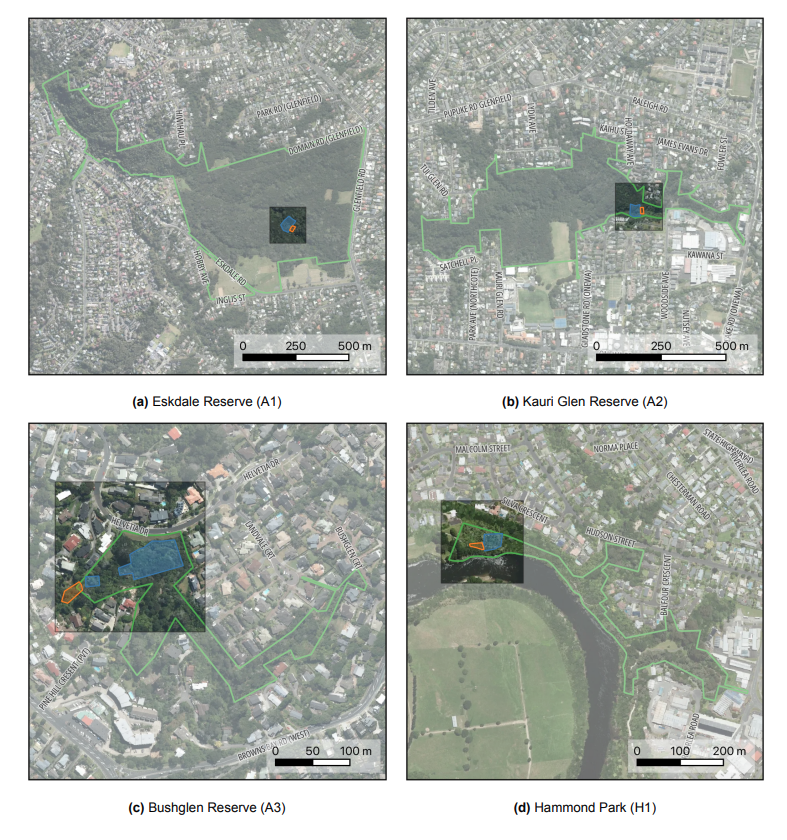
\includegraphics[keepaspectratio]{../2_1_figures/annex/sites.png}}

}

\caption{\label{sfig-sites_extent_overview}Inset maps showing the
location of the maps of Figure~\ref{fig-sites_extent}. The map shows
park extent (green), training (blue) and test (orange) zones used for
model evaluation; site areas are listed in Table~\ref{tbl-overview}.
Basemap: LINZ aerial imagery under CC BY 4.0. Park extents: Auckland
Council (A1--A3) and Waikato OneView (H1) under CC BY 4.0.}

\end{sfig}%

\section*{Multispectral Reflectance
Calibration}\label{multispectral-reflectance-calibration}

\begin{sfig}[H]

\begin{minipage}{0.10\linewidth}
~\end{minipage}%
%
\begin{minipage}{0.80\linewidth}

\pandocbounded{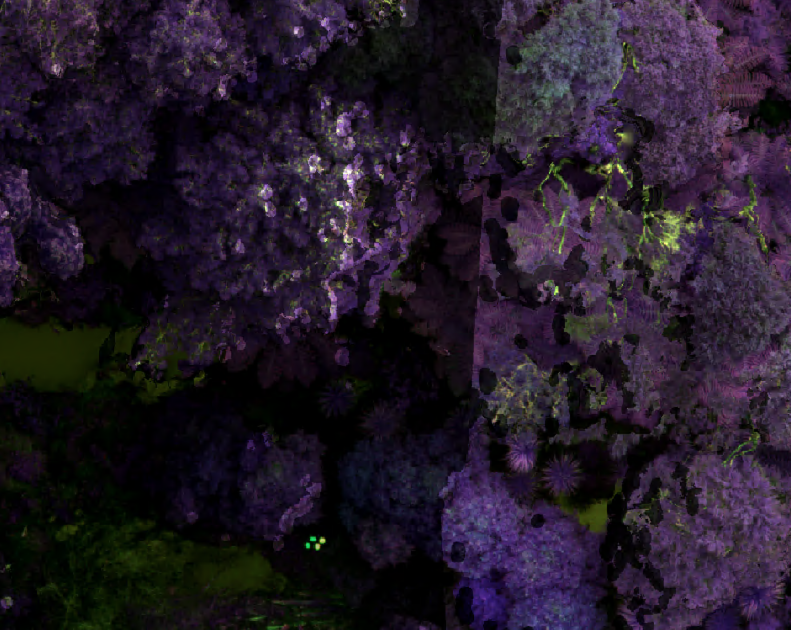
\includegraphics[keepaspectratio]{../2_1_figures/annex/ms_seamline.png}}

\end{minipage}%
%
\begin{minipage}{0.10\linewidth}
~\end{minipage}%

\caption{\label{sfig-ms_seamline}Example of different reflectance on
calibrated \hyperref[acronyms_MS]{MS} imagery from preliminary flights
in April, most likely caused by changing cloud coverage, leading to the
decision to carry out flights again with more consistent exposure to
ensure high-quality data.}

\end{sfig}%

\section*{Calibration Panel Histogram
Analysis}\label{calibration-panel-histogram-analysis}

\begin{sfig}[H]

\begin{minipage}{0.14\linewidth}
~\end{minipage}%
%
\begin{minipage}{0.71\linewidth}

\pandocbounded{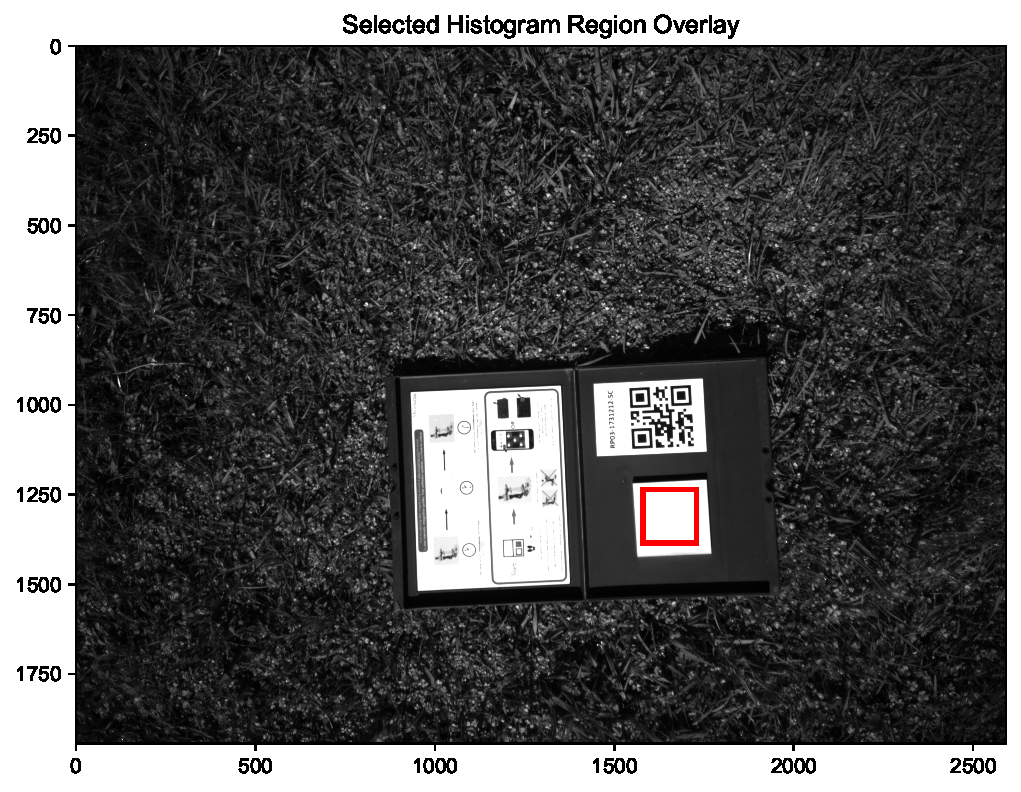
\includegraphics[keepaspectratio]{complete_thesis_files/figure-pdf/cell-12-output-1.pdf}}

\textbf{(a)} Histogram area\end{minipage}%
%
\begin{minipage}{0.14\linewidth}
~\end{minipage}%
\newline
\begin{minipage}{0.48\linewidth}

\pandocbounded{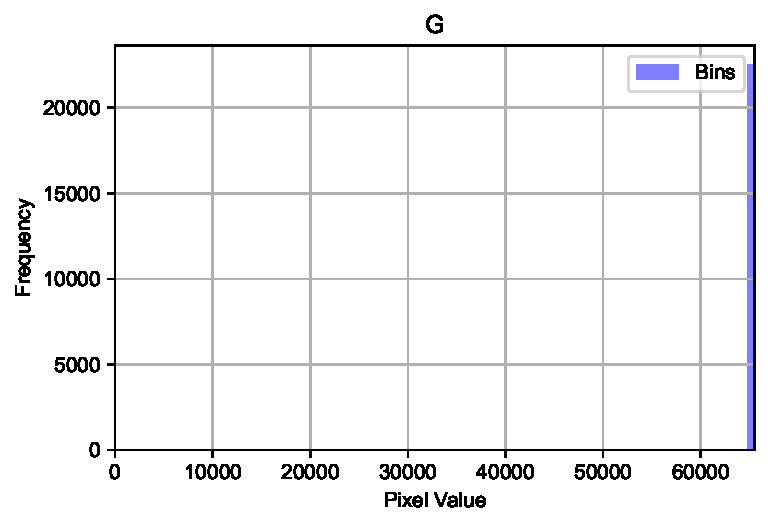
\includegraphics[keepaspectratio]{complete_thesis_files/figure-pdf/cell-13-output-1.pdf}}

\textbf{(b)} \hyperref[acronyms_G]{G} band, which is fully
saturated.\end{minipage}%
%
\begin{minipage}{0.05\linewidth}
~\end{minipage}%
%
\begin{minipage}{0.48\linewidth}

\pandocbounded{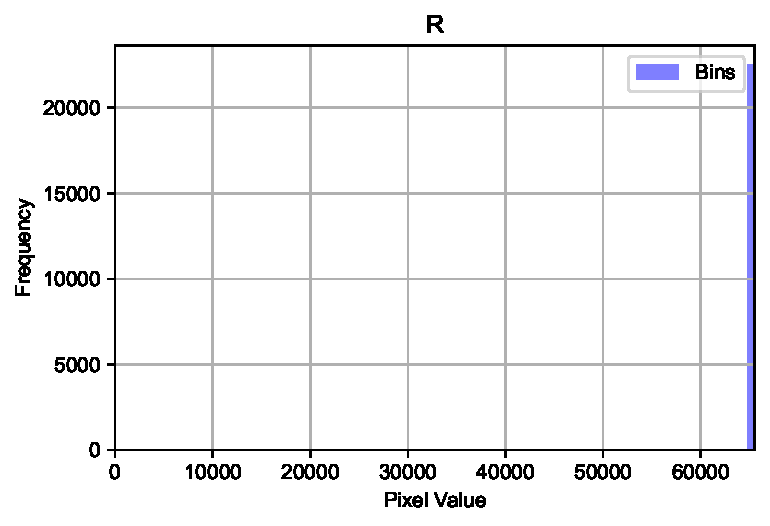
\includegraphics[keepaspectratio]{complete_thesis_files/figure-pdf/cell-14-output-1.pdf}}

\textbf{(c)} \hyperref[acronyms_R]{R} band, which is fully
saturated.\end{minipage}%
\newline
\begin{minipage}{0.48\linewidth}

\pandocbounded{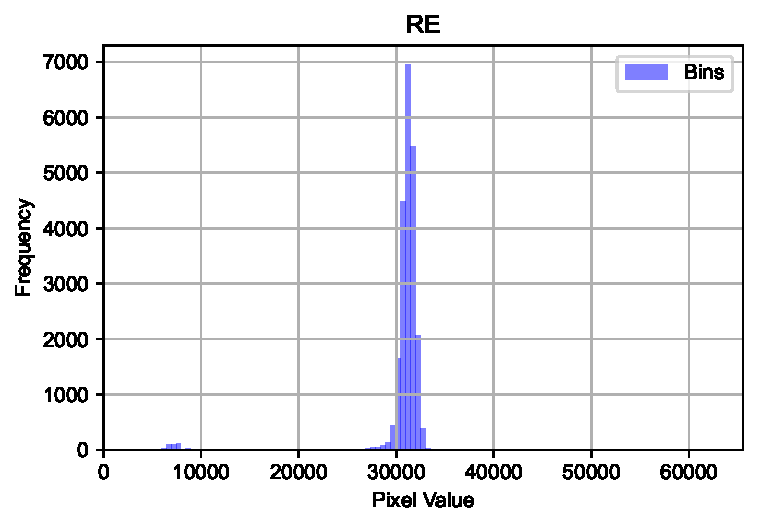
\includegraphics[keepaspectratio]{complete_thesis_files/figure-pdf/cell-15-output-1.pdf}}

\textbf{(d)} \hyperref[acronyms_RE]{RE} band, which can be used for
calibration.\end{minipage}%
%
\begin{minipage}{0.05\linewidth}
~\end{minipage}%
%
\begin{minipage}{0.48\linewidth}

\pandocbounded{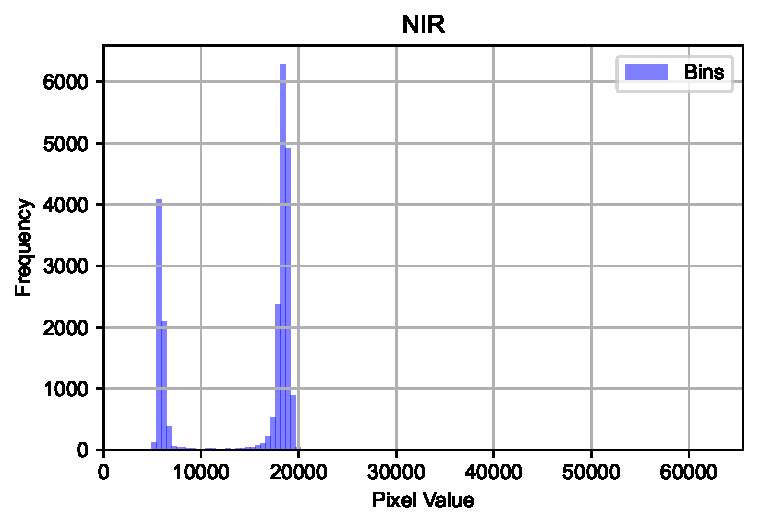
\includegraphics[keepaspectratio]{complete_thesis_files/figure-pdf/cell-16-output-1.pdf}}

\textbf{(e)} \hyperref[acronyms_NIR]{NIR} band, which can be used for
calibration.\end{minipage}%

\caption{\label{sfig-crp_hist}Histogram of the
\hyperref[acronyms_CRP]{CRP} within the calibrated area (histogram is
calculated only for the area in the red box). Bands
\hyperref[acronyms_G]{G} and \hyperref[acronyms_R]{R} (\textbf{b},
\textbf{c}) are fully saturated and therefore cannot lead to proper
calibration.}

\end{sfig}%

\section*{Image Metadata and Exposure
Settings}\label{image-metadata-and-exposure-settings}

\begin{sfig}[H]

\centering{

\begin{figure}[H]

\begin{minipage}{0.50\linewidth}
\pandocbounded{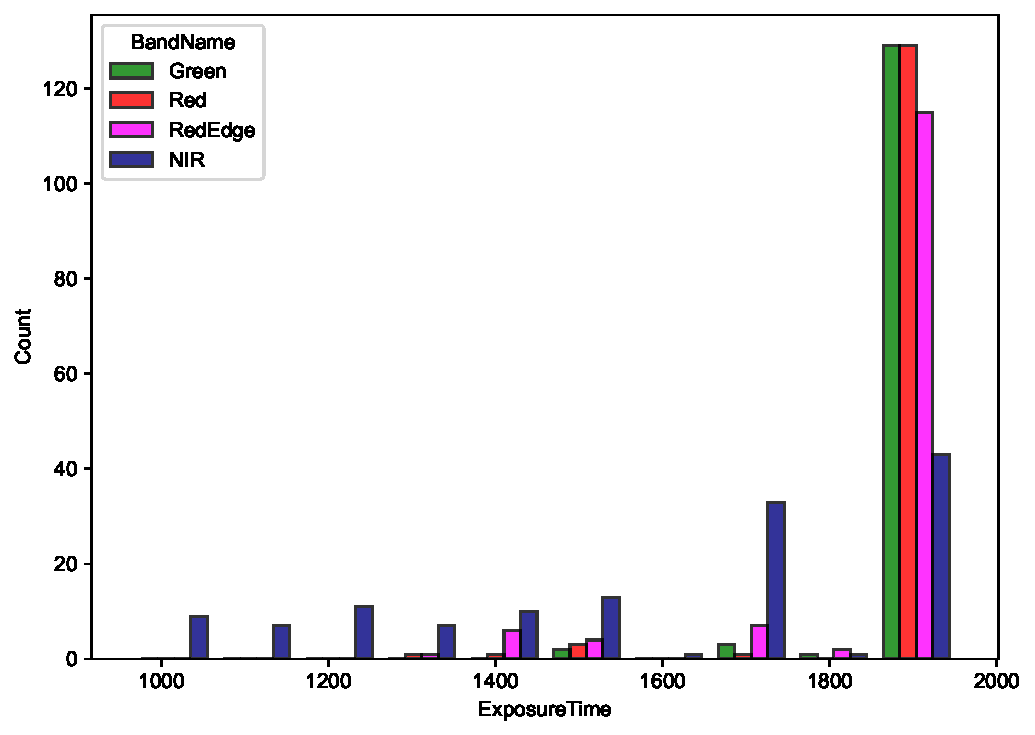
\includegraphics[keepaspectratio]{complete_thesis_files/figure-pdf/cell-17-output-1.pdf}}\end{minipage}%
%
\begin{minipage}{0.50\linewidth}
\pandocbounded{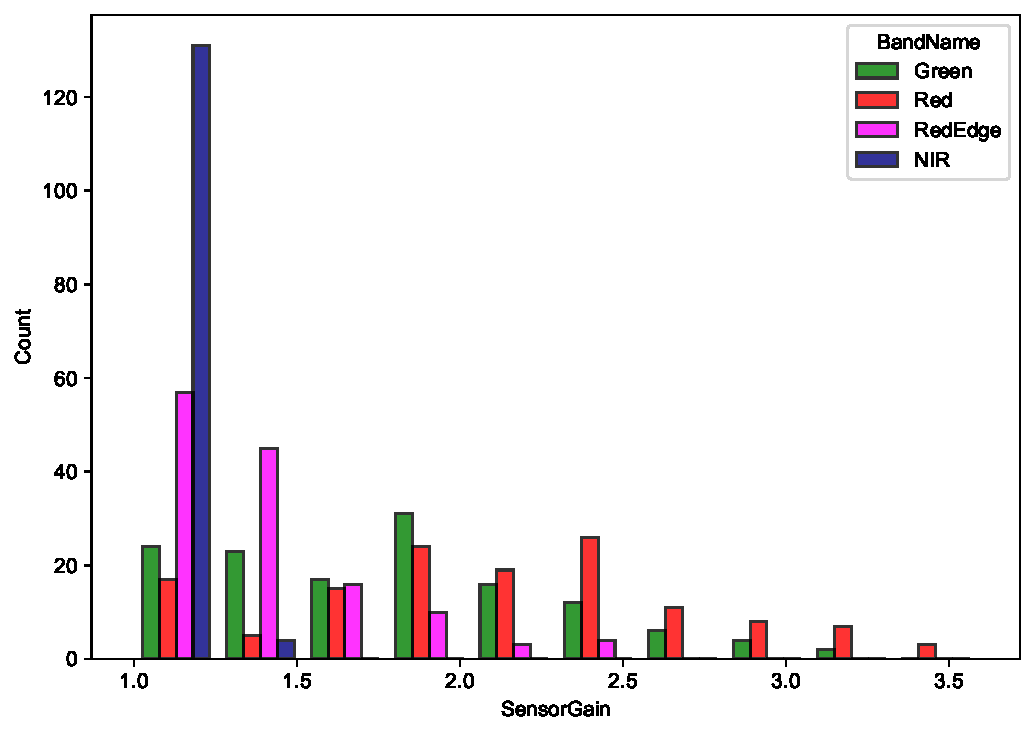
\includegraphics[keepaspectratio]{complete_thesis_files/figure-pdf/cell-17-output-2.pdf}}\end{minipage}%

\end{figure}%

}

\caption{\label{sfig-exposure}Metadata for site A2 showing exposure time
and sensor gain, showing that the auto-settings of the
\hyperref[acronyms_M3M]{M3M} are inconsistent during a capture.}

\end{sfig}%

\section*{Processing Artefacts}\label{processing-artefacts}

\begin{sfig}[H]

\centering{

\pandocbounded{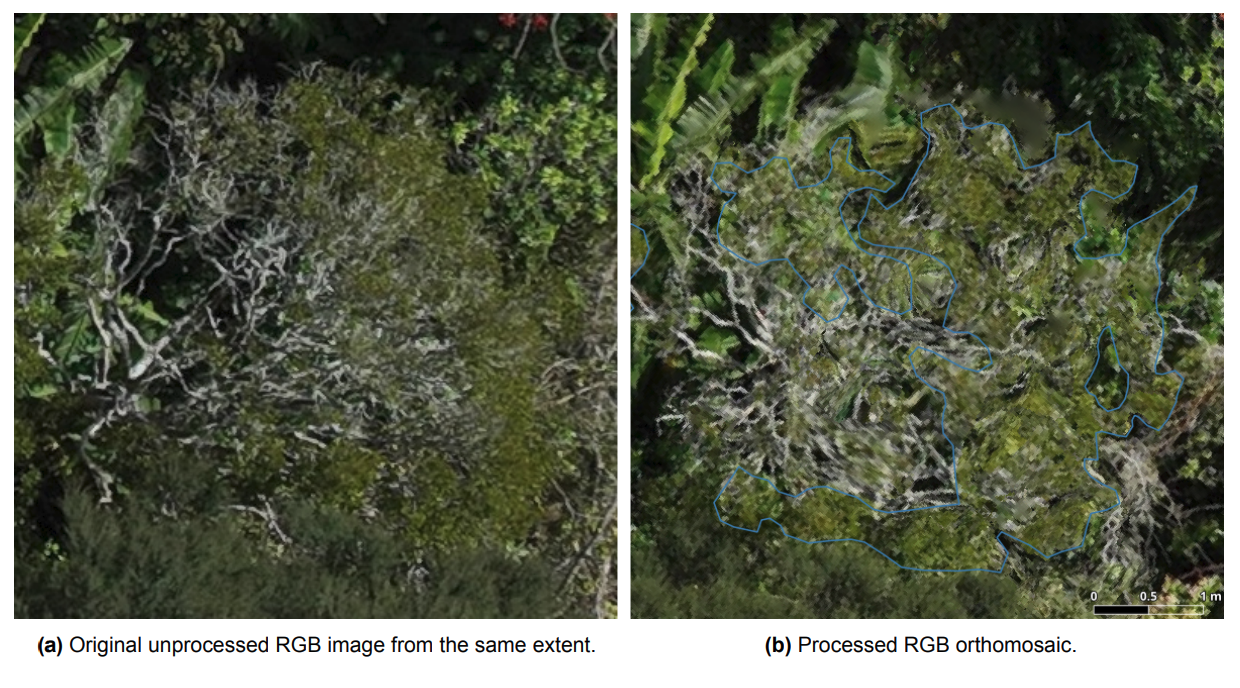
\includegraphics[keepaspectratio]{../2_1_figures/annex/artefacts_combined.png}}

}

\caption{\label{sfig-artefacts}Example of artefacts on processed
\hyperref[acronyms_RGB]{RGB} orthomosaic (\textbf{b}), and the same
extent extracted from the raw image (before processing) without
artefacts (\textbf{a}).}

\end{sfig}%

\section*{Training Dataset
Characteristics}\label{training-dataset-characteristics}

\begin{stbl}[H]

\caption{\label{stbl-class_distribution}Dataset summary with class
distribution of training (80\%) and validation split (20\%) showing tile
counts and \hyperref[acronyms_SM]{\emph{S. maire}} pixel percentages for
each reserve.}

\centering{

\begin{longtable*}[]{@{}
  >{\raggedright\arraybackslash}p{(\linewidth - 8\tabcolsep) * \real{0.1343}}
  >{\raggedright\arraybackslash}p{(\linewidth - 8\tabcolsep) * \real{0.2090}}
  >{\raggedright\arraybackslash}p{(\linewidth - 8\tabcolsep) * \real{0.2537}}
  >{\raggedright\arraybackslash}p{(\linewidth - 8\tabcolsep) * \real{0.1791}}
  >{\raggedright\arraybackslash}p{(\linewidth - 8\tabcolsep) * \real{0.2239}}@{}}
\toprule\noalign{}
\begin{minipage}[b]{\linewidth}\raggedright
Reserve
\end{minipage} & \begin{minipage}[b]{\linewidth}\raggedright
Train Images
\end{minipage} & \begin{minipage}[b]{\linewidth}\raggedright
Train Maire (\%)
\end{minipage} & \begin{minipage}[b]{\linewidth}\raggedright
Val Images
\end{minipage} & \begin{minipage}[b]{\linewidth}\raggedright
Val Maire (\%)
\end{minipage} \\
\midrule\noalign{}
\endhead
\bottomrule\noalign{}
\endlastfoot
A1 & 26 & 3.34 & 8 & 3.94 \\
A2 & 9 & 2.37 & 3 & 3.96 \\
A3 & 21 & 5.64 & 6 & 6.21 \\
H1 & 6 & 2.19 & 3 & 5.60 \\
Combined & 65 & 4.58 & 17 & 2.35 \\
\end{longtable*}

}

\end{stbl}%

\section*{Model Performance and Hyperparameter
Exploration}\label{model-performance-and-hyperparameter-exploration}

\subsection*{\texorpdfstring{Learning Rate Example:
5×10\textsuperscript{-5}}{Learning Rate Example: 5×10-5}}\label{learning-rate-example-510-5}

\begin{sfig}[H]

\centering{

\pandocbounded{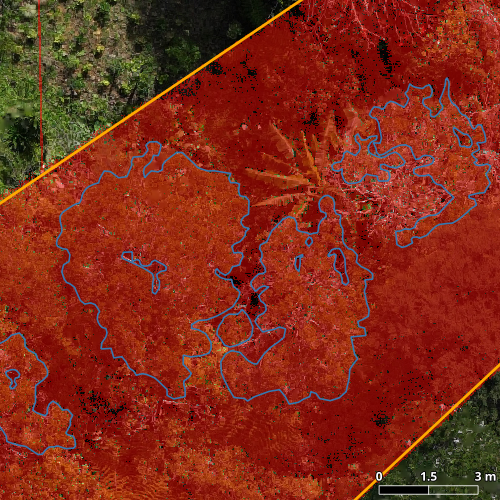
\includegraphics[keepaspectratio]{../2_1_figures/annex/LRe05.png}}

}

\caption{\label{sfig-LR5e-5}Example of random predictions from a model
trained with \hyperref[acronyms_LR]{LR} 5x10\textsuperscript{-5}. Orange
shows the extent of the test area, blue are the
\hyperref[acronyms_SM]{\emph{S. maire}} annotations and red are the
model predictions.}

\end{sfig}%

\section*{Training Dashboards}\label{training-dashboards}

\begin{sfig}[H]

\centering{

\pandocbounded{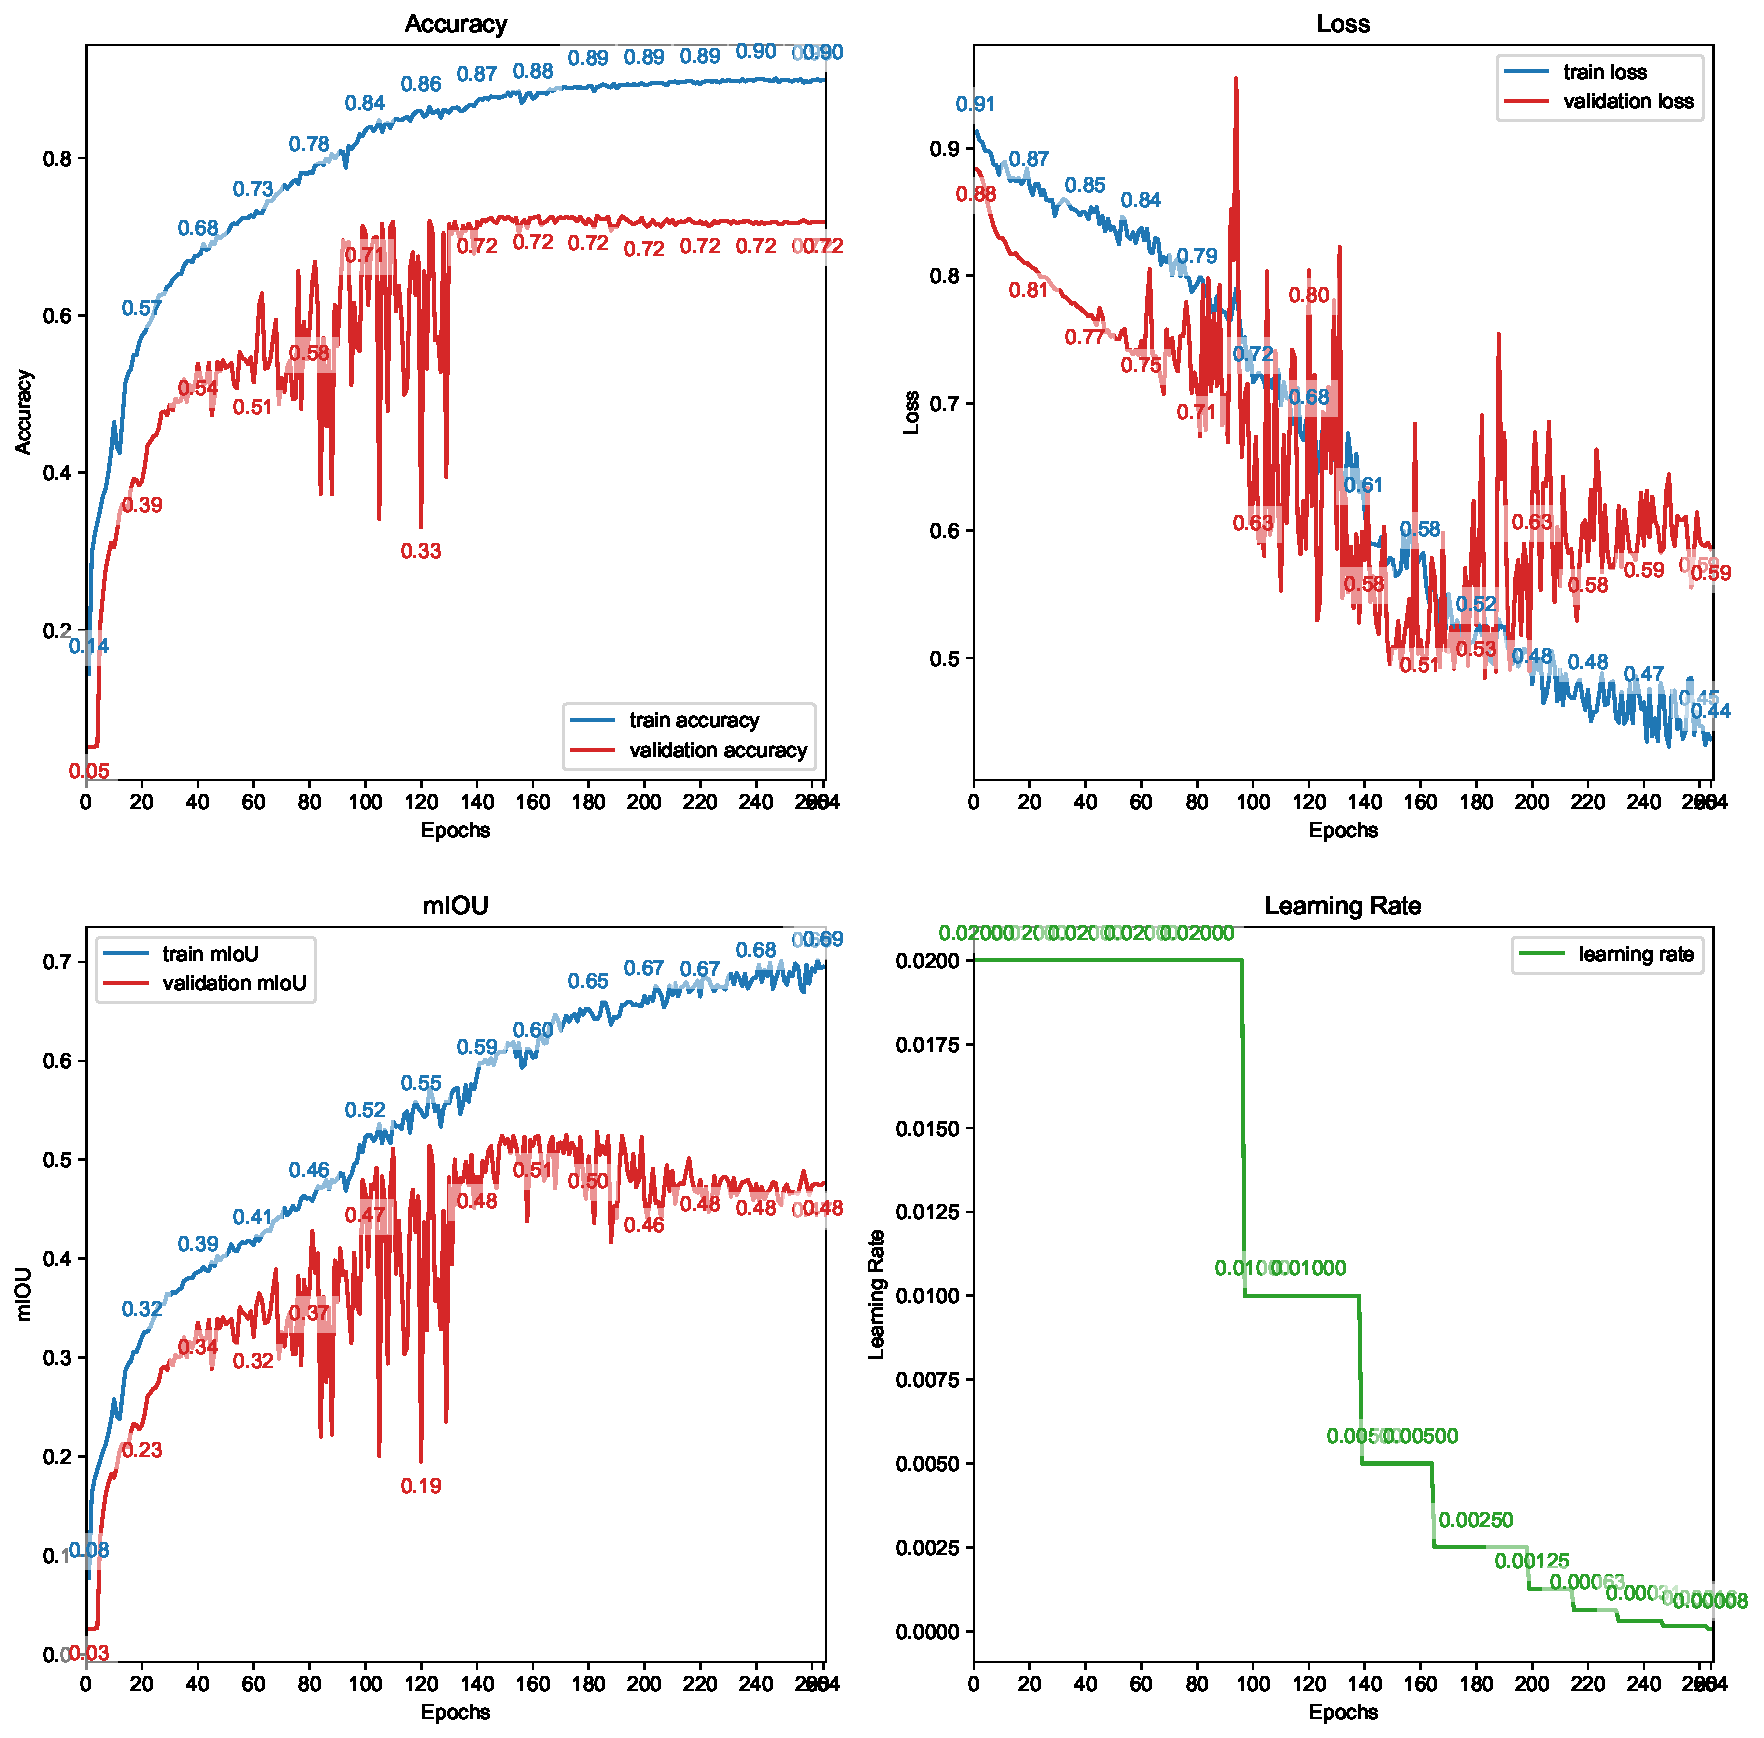
\includegraphics[keepaspectratio]{complete_thesis_files/figure-pdf/cell-20-output-1.pdf}}

}

\caption{\label{sfig-train_metrics_best}Train metrics from the best
performing single-site model for site A2 trained on relatively
calibrated \hyperref[acronyms_MS]{MS} data using Dice Loss.}

\end{sfig}%

\begin{sfig}[H]

\centering{

\pandocbounded{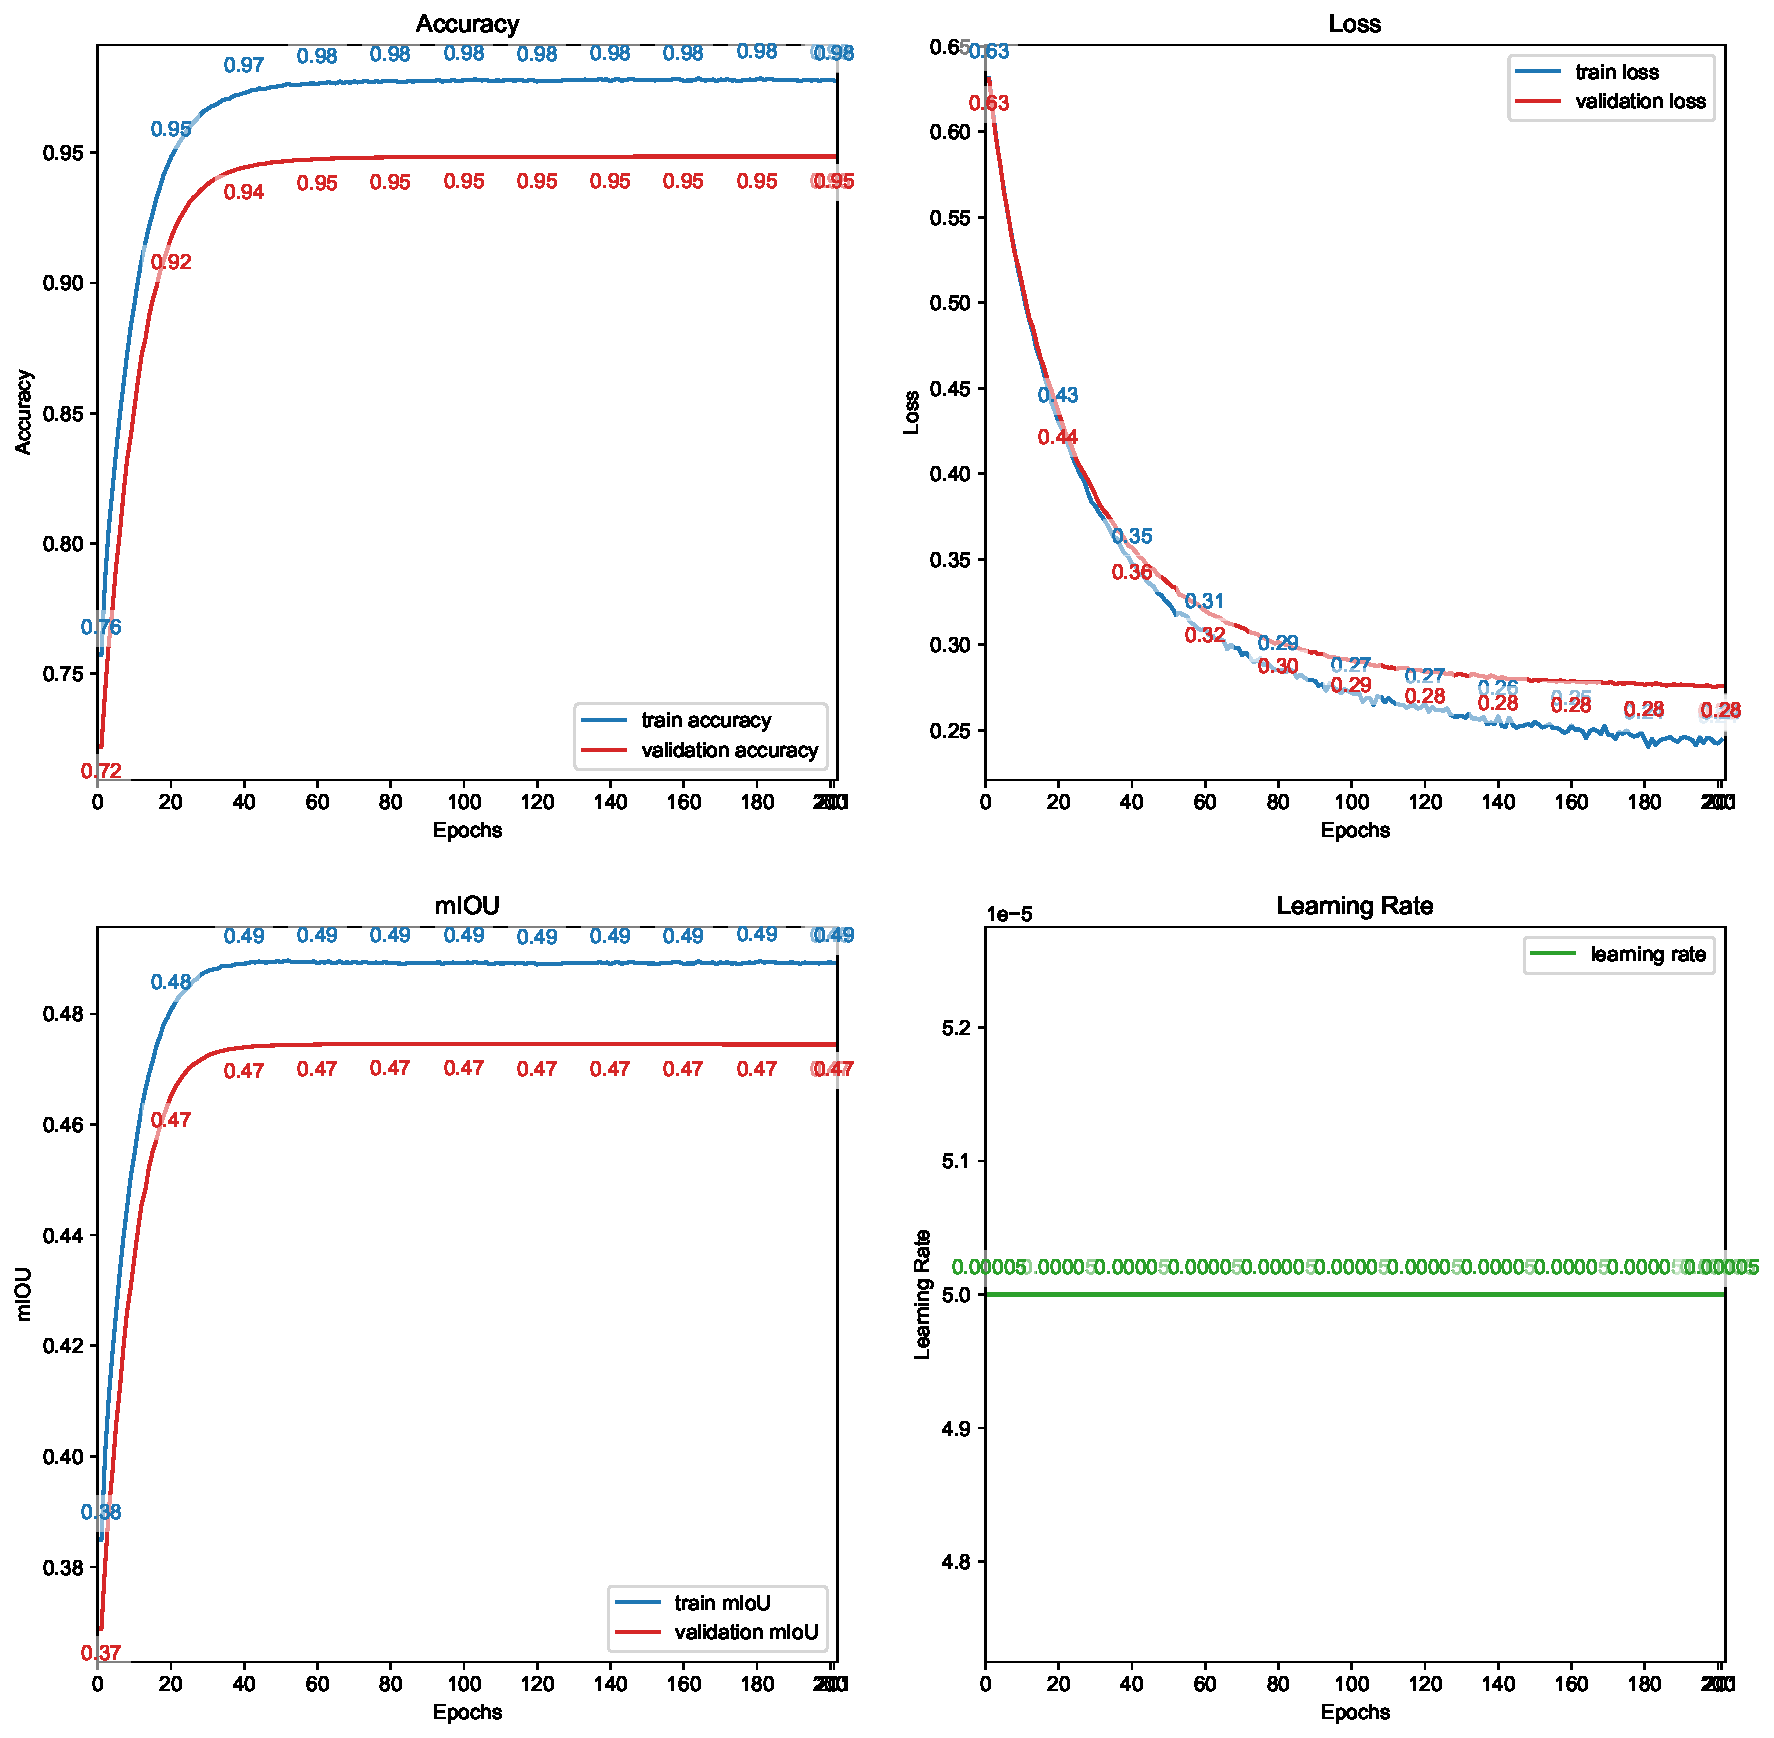
\includegraphics[keepaspectratio]{complete_thesis_files/figure-pdf/cell-21-output-1.pdf}}

}

\caption{\label{sfig-train_metrics_multi_site}Train metrics from
multi-site model trained on all sites with no training effect. Model was
trained with a \hyperref[acronyms_LR]{LR} of 5x10\textsuperscript{-5}.}

\end{sfig}%

\begin{stbl}[H]

\caption{\label{stbl-model_type}Overall best performing parameters for
multi-site.}

\centering{

\begin{longtable*}[]{@{}
  >{\raggedright\arraybackslash}p{(\linewidth - 10\tabcolsep) * \real{0.3684}}
  >{\raggedright\arraybackslash}p{(\linewidth - 10\tabcolsep) * \real{0.1579}}
  >{\raggedright\arraybackslash}p{(\linewidth - 10\tabcolsep) * \real{0.0789}}
  >{\raggedright\arraybackslash}p{(\linewidth - 10\tabcolsep) * \real{0.1316}}
  >{\raggedright\arraybackslash}p{(\linewidth - 10\tabcolsep) * \real{0.1316}}
  >{\raggedright\arraybackslash}p{(\linewidth - 10\tabcolsep) * \real{0.1316}}@{}}
\toprule\noalign{}
\begin{minipage}[b]{\linewidth}\raggedright
Bands
\end{minipage} & \begin{minipage}[b]{\linewidth}\raggedright
Loss
\end{minipage} & \begin{minipage}[b]{\linewidth}\raggedright
W
\end{minipage} & \begin{minipage}[b]{\linewidth}\raggedright
LR
\end{minipage} & \begin{minipage}[b]{\linewidth}\raggedright
F1
\end{minipage} & \begin{minipage}[b]{\linewidth}\raggedright
IoU
\end{minipage} \\
\midrule\noalign{}
\endhead
\bottomrule\noalign{}
\endlastfoot
RGB & \hyperref[acronyms_DICE]{\(L_{Dice}\)} & 1 & 0.02 & 0.56±0.14 &
0.40±0.14 \\
MS\(_{rel}\) & \hyperref[acronyms_DICE]{\(L_{Dice}\)} & 1 & 0.02 &
0.54±0.25 & 0.40±0.23 \\
RGB & \hyperref[acronyms_WBCE_D]{\(L_{c}\)} & 50 & 0.02 & 0.52±0.14 &
0.36±0.12 \\
MS\(_{rel}\) & \hyperref[acronyms_WBCE_D]{\(L_{c}\)} & 50 & 0.02 &
0.50±0.17 & 0.34±0.14 \\
RGB & \hyperref[acronyms_WBCE_D]{\(L_{c}\)} & 10 & 0.02 & 0.50±0.20 &
0.35±0.19 \\
\end{longtable*}

}

\end{stbl}%

\subsection*{Best Performing Models per
Site}\label{sec-top_models_individual}

\begin{stbl}[H]

\caption{\label{stbl-best_models_single_site_ESK}Overall best performing
models for site A1.}

\centering{

\begin{longtable*}[]{@{}
  >{\raggedright\arraybackslash}p{(\linewidth - 16\tabcolsep) * \real{0.1552}}
  >{\raggedright\arraybackslash}p{(\linewidth - 16\tabcolsep) * \real{0.2414}}
  >{\raggedright\arraybackslash}p{(\linewidth - 16\tabcolsep) * \real{0.1034}}
  >{\raggedright\arraybackslash}p{(\linewidth - 16\tabcolsep) * \real{0.0517}}
  >{\raggedright\arraybackslash}p{(\linewidth - 16\tabcolsep) * \real{0.0862}}
  >{\raggedright\arraybackslash}p{(\linewidth - 16\tabcolsep) * \real{0.0862}}
  >{\raggedright\arraybackslash}p{(\linewidth - 16\tabcolsep) * \real{0.0862}}
  >{\raggedright\arraybackslash}p{(\linewidth - 16\tabcolsep) * \real{0.1034}}
  >{\raggedright\arraybackslash}p{(\linewidth - 16\tabcolsep) * \real{0.0862}}@{}}
\toprule\noalign{}
\begin{minipage}[b]{\linewidth}\raggedright
Reserve
\end{minipage} & \begin{minipage}[b]{\linewidth}\raggedright
Bands
\end{minipage} & \begin{minipage}[b]{\linewidth}\raggedright
Loss
\end{minipage} & \begin{minipage}[b]{\linewidth}\raggedright
W
\end{minipage} & \begin{minipage}[b]{\linewidth}\raggedright
LR
\end{minipage} & \begin{minipage}[b]{\linewidth}\raggedright
F1
\end{minipage} & \begin{minipage}[b]{\linewidth}\raggedright
IoU
\end{minipage} & \begin{minipage}[b]{\linewidth}\raggedright
Prec
\end{minipage} & \begin{minipage}[b]{\linewidth}\raggedright
Rec
\end{minipage} \\
\midrule\noalign{}
\endhead
\bottomrule\noalign{}
\endlastfoot
A1 & MS\(_{rel}\) & \hyperref[acronyms_WBCE_D]{\(L_{c}\)} & 50 & 0.02 &
0.65 & 0.48 & 0.52 & 0.87 \\
A1 & MS+IND\(_{rel}\) & \hyperref[acronyms_WBCE_D]{\(L_{c}\)} & 10 &
0.02 & 0.64 & 0.47 & 0.51 & 0.87 \\
A1 & RGB & \hyperref[acronyms_WBCE_D]{\(L_{c}\)} & 50 & 0.02 & 0.62 &
0.45 & 0.51 & 0.80 \\
A1 & MS\(_{rel}\) & \hyperref[acronyms_DICE]{\(L_{Dice}\)} & 1 & 0.02 &
0.61 & 0.44 & 0.70 & 0.55 \\
A1 & RGB & \hyperref[acronyms_DICE]{\(L_{Dice}\)} & 1 & 0.02 & 0.60 &
0.43 & 0.46 & 0.87 \\
A1 & RGB & \hyperref[acronyms_WBCE]{\(L_{WBCE}\)} & 10 & 0.02 & 0.60 &
0.43 & 0.52 & 0.72 \\
A1 & MS\(_{rel}\) & \hyperref[acronyms_WBCE]{\(L_{WBCE}\)} & 50 & 0.02 &
0.59 & 0.42 & 0.50 & 0.72 \\
A1 & MS\(_{rel}\) & \hyperref[acronyms_WBCE_D]{\(L_{c}\)} & 1 & 0.02 &
0.57 & 0.40 & 0.62 & 0.52 \\
A1 & RGB & \hyperref[acronyms_WBCE]{\(L_{WBCE}\)} & 50 & 0.02 & 0.56 &
0.38 & 0.41 & 0.86 \\
A1 & RGB & \hyperref[acronyms_WBCE_D]{\(L_{c}\)} & 10 & 0.02 & 0.55 &
0.38 & 0.45 & 0.72 \\
\end{longtable*}

}

\end{stbl}%

\begin{stbl}[H]

\caption{\label{stbl-best_models_single_site_KAU}Overall best performing
models for site A2.}

\centering{

\begin{longtable*}[]{@{}
  >{\raggedright\arraybackslash}p{(\linewidth - 16\tabcolsep) * \real{0.1552}}
  >{\raggedright\arraybackslash}p{(\linewidth - 16\tabcolsep) * \real{0.2414}}
  >{\raggedright\arraybackslash}p{(\linewidth - 16\tabcolsep) * \real{0.1034}}
  >{\raggedright\arraybackslash}p{(\linewidth - 16\tabcolsep) * \real{0.0517}}
  >{\raggedright\arraybackslash}p{(\linewidth - 16\tabcolsep) * \real{0.0862}}
  >{\raggedright\arraybackslash}p{(\linewidth - 16\tabcolsep) * \real{0.0862}}
  >{\raggedright\arraybackslash}p{(\linewidth - 16\tabcolsep) * \real{0.0862}}
  >{\raggedright\arraybackslash}p{(\linewidth - 16\tabcolsep) * \real{0.1034}}
  >{\raggedright\arraybackslash}p{(\linewidth - 16\tabcolsep) * \real{0.0862}}@{}}
\toprule\noalign{}
\begin{minipage}[b]{\linewidth}\raggedright
Reserve
\end{minipage} & \begin{minipage}[b]{\linewidth}\raggedright
Bands
\end{minipage} & \begin{minipage}[b]{\linewidth}\raggedright
Loss
\end{minipage} & \begin{minipage}[b]{\linewidth}\raggedright
W
\end{minipage} & \begin{minipage}[b]{\linewidth}\raggedright
LR
\end{minipage} & \begin{minipage}[b]{\linewidth}\raggedright
F1
\end{minipage} & \begin{minipage}[b]{\linewidth}\raggedright
IoU
\end{minipage} & \begin{minipage}[b]{\linewidth}\raggedright
Prec
\end{minipage} & \begin{minipage}[b]{\linewidth}\raggedright
Rec
\end{minipage} \\
\midrule\noalign{}
\endhead
\bottomrule\noalign{}
\endlastfoot
A2 & RGB & \hyperref[acronyms_DICE]{\(L_{Dice}\)} & 1 & 0.02 & 0.46 &
0.30 & 0.45 & 0.48 \\
A2 & RGB & \hyperref[acronyms_WBCE_D]{\(L_{c}\)} & 50 & 0.02 & 0.44 &
0.28 & 0.65 & 0.33 \\
A2 & RGB & \hyperref[acronyms_WBCE_D]{\(L_{c}\)} & 10 & 0.02 & 0.41 &
0.26 & 0.42 & 0.40 \\
A2 & RGB & \hyperref[acronyms_WBCE_D]{\(L_{c}\)} & 1 & 0.02 & 0.35 &
0.21 & 0.67 & 0.24 \\
A2 & MS\(_{rel}\) & \hyperref[acronyms_WBCE_D]{\(L_{c}\)} & 1 & 0.02 &
0.30 & 0.18 & 0.87 & 0.18 \\
A2 & RGB & \hyperref[acronyms_WBCE_D]{\(L_{c}\)} & 50 &
5x10\textsuperscript{-5} & 0.28 & 0.16 & 0.20 & 0.48 \\
A2 & MS\(_{rel}\) & \hyperref[acronyms_WBCE]{\(L_{WBCE}\)} & 50 & 0.02 &
0.26 & 0.15 & 0.45 & 0.19 \\
A2 & RGB & \hyperref[acronyms_WBCE]{\(L_{WBCE}\)} & 50 & 0.02 & 0.25 &
0.14 & 0.23 & 0.27 \\
A2 & MS\(_{rel}\) & \hyperref[acronyms_WBCE_D]{\(L_{c}\)} & 50 & 0.02 &
0.25 & 0.14 & 0.39 & 0.18 \\
A2 & MS\(_{rel}\) & \hyperref[acronyms_WBCE]{\(L_{WBCE}\)} & 10 & 0.02 &
0.23 & 0.13 & 0.85 & 0.13 \\
\end{longtable*}

}

\end{stbl}%

\begin{stbl}[H]

\caption{\label{stbl-best_models_single_site_BUS}Overall best performing
models for site A3.}

\centering{

\begin{longtable*}[]{@{}
  >{\raggedright\arraybackslash}p{(\linewidth - 16\tabcolsep) * \real{0.1552}}
  >{\raggedright\arraybackslash}p{(\linewidth - 16\tabcolsep) * \real{0.2414}}
  >{\raggedright\arraybackslash}p{(\linewidth - 16\tabcolsep) * \real{0.1034}}
  >{\raggedright\arraybackslash}p{(\linewidth - 16\tabcolsep) * \real{0.0517}}
  >{\raggedright\arraybackslash}p{(\linewidth - 16\tabcolsep) * \real{0.0862}}
  >{\raggedright\arraybackslash}p{(\linewidth - 16\tabcolsep) * \real{0.0862}}
  >{\raggedright\arraybackslash}p{(\linewidth - 16\tabcolsep) * \real{0.0862}}
  >{\raggedright\arraybackslash}p{(\linewidth - 16\tabcolsep) * \real{0.1034}}
  >{\raggedright\arraybackslash}p{(\linewidth - 16\tabcolsep) * \real{0.0862}}@{}}
\toprule\noalign{}
\begin{minipage}[b]{\linewidth}\raggedright
Reserve
\end{minipage} & \begin{minipage}[b]{\linewidth}\raggedright
Bands
\end{minipage} & \begin{minipage}[b]{\linewidth}\raggedright
Loss
\end{minipage} & \begin{minipage}[b]{\linewidth}\raggedright
W
\end{minipage} & \begin{minipage}[b]{\linewidth}\raggedright
LR
\end{minipage} & \begin{minipage}[b]{\linewidth}\raggedright
F1
\end{minipage} & \begin{minipage}[b]{\linewidth}\raggedright
IoU
\end{minipage} & \begin{minipage}[b]{\linewidth}\raggedright
Prec
\end{minipage} & \begin{minipage}[b]{\linewidth}\raggedright
Rec
\end{minipage} \\
\midrule\noalign{}
\endhead
\bottomrule\noalign{}
\endlastfoot
A3 & MS\(_{rel}\) & \hyperref[acronyms_DICE]{\(L_{Dice}\)} & 1 & 0.02 &
0.81 & 0.68 & 0.74 & 0.88 \\
A3 & MS\(_{rel}\) & \hyperref[acronyms_WBCE_D]{\(L_{c}\)} & 1 & 0.02 &
0.80 & 0.67 & 0.72 & 0.89 \\
A3 & RGB & \hyperref[acronyms_WBCE]{\(L_{WBCE}\)} & 10 & 0.02 & 0.77 &
0.62 & 0.68 & 0.87 \\
A3 & RGB & \hyperref[acronyms_WBCE_D]{\(L_{c}\)} & 10 & 0.02 & 0.75 &
0.60 & 0.74 & 0.76 \\
A3 & RGB & \hyperref[acronyms_DICE]{\(L_{Dice}\)} & 1 & 0.02 & 0.74 &
0.59 & 0.64 & 0.87 \\
A3 & RGB & \hyperref[acronyms_WBCE_D]{\(L_{c}\)} & 1 & 0.02 & 0.72 &
0.57 & 0.62 & 0.86 \\
A3 & MS\(_{rel}\) & \hyperref[acronyms_WBCE_D]{\(L_{c}\)} & 10 & 0.02 &
0.66 & 0.49 & 0.51 & 0.91 \\
A3 & RGB & \hyperref[acronyms_WBCE_D]{\(L_{c}\)} & 50 & 0.02 & 0.65 &
0.48 & 0.52 & 0.86 \\
A3 & MS\(_{rel}\) & \hyperref[acronyms_WBCE]{\(L_{WBCE}\)} & 10 & 0.02 &
0.64 & 0.47 & 0.55 & 0.77 \\
A3 & IND\(_{rel}\) & \hyperref[acronyms_WBCE_D]{\(L_{c}\)} & 10 & 0.02 &
0.64 & 0.47 & 0.49 & 0.92 \\
\end{longtable*}

}

\end{stbl}%

\begin{stbl}[H]

\caption{\label{stbl-best_models_single_site_HAM}Overall best performing
models for site H1.}

\centering{

\begin{longtable*}[]{@{}
  >{\raggedright\arraybackslash}p{(\linewidth - 16\tabcolsep) * \real{0.1552}}
  >{\raggedright\arraybackslash}p{(\linewidth - 16\tabcolsep) * \real{0.2414}}
  >{\raggedright\arraybackslash}p{(\linewidth - 16\tabcolsep) * \real{0.1034}}
  >{\raggedright\arraybackslash}p{(\linewidth - 16\tabcolsep) * \real{0.0517}}
  >{\raggedright\arraybackslash}p{(\linewidth - 16\tabcolsep) * \real{0.0862}}
  >{\raggedright\arraybackslash}p{(\linewidth - 16\tabcolsep) * \real{0.0862}}
  >{\raggedright\arraybackslash}p{(\linewidth - 16\tabcolsep) * \real{0.0862}}
  >{\raggedright\arraybackslash}p{(\linewidth - 16\tabcolsep) * \real{0.1034}}
  >{\raggedright\arraybackslash}p{(\linewidth - 16\tabcolsep) * \real{0.0862}}@{}}
\toprule\noalign{}
\begin{minipage}[b]{\linewidth}\raggedright
Reserve
\end{minipage} & \begin{minipage}[b]{\linewidth}\raggedright
Bands
\end{minipage} & \begin{minipage}[b]{\linewidth}\raggedright
Loss
\end{minipage} & \begin{minipage}[b]{\linewidth}\raggedright
W
\end{minipage} & \begin{minipage}[b]{\linewidth}\raggedright
LR
\end{minipage} & \begin{minipage}[b]{\linewidth}\raggedright
F1
\end{minipage} & \begin{minipage}[b]{\linewidth}\raggedright
IoU
\end{minipage} & \begin{minipage}[b]{\linewidth}\raggedright
Prec
\end{minipage} & \begin{minipage}[b]{\linewidth}\raggedright
Rec
\end{minipage} \\
\midrule\noalign{}
\endhead
\bottomrule\noalign{}
\endlastfoot
H1 & MS\(_{rel}\) & \hyperref[acronyms_WBCE_D]{\(L_{c}\)} & 10 & 0.02 &
0.59 & 0.42 & 0.44 & 0.89 \\
H1 & MS\(_{rel}\) & \hyperref[acronyms_WBCE_D]{\(L_{c}\)} & 50 & 0.02 &
0.56 & 0.38 & 0.42 & 0.82 \\
H1 & MS\(_{rel}\) & \hyperref[acronyms_DICE]{\(L_{Dice}\)} & 1 & 0.02 &
0.53 & 0.36 & 0.39 & 0.83 \\
H1 & MS\(_{rel}\) & \hyperref[acronyms_WBCE]{\(L_{WBCE}\)} & 10 & 0.02 &
0.48 & 0.32 & 0.32 & 0.94 \\
H1 & MS+IND\(_{rel}\) & \hyperref[acronyms_WBCE_D]{\(L_{c}\)} & 10 &
0.02 & 0.46 & 0.30 & 0.38 & 0.59 \\
H1 & RGB & \hyperref[acronyms_DICE]{\(L_{Dice}\)} & 1 & 0.02 & 0.45 &
0.29 & 0.32 & 0.79 \\
H1 & IND\(_{rel}\) & \hyperref[acronyms_WBCE_D]{\(L_{c}\)} & 10 & 0.02 &
0.42 & 0.27 & 0.28 & 0.80 \\
H1 & RGB & \hyperref[acronyms_WBCE]{\(L_{WBCE}\)} & 10 & 0.02 & 0.40 &
0.25 & 0.31 & 0.54 \\
H1 & MS\(_{rel}\) & \hyperref[acronyms_WBCE]{\(L_{WBCE}\)} & 50 & 0.02 &
0.39 & 0.24 & 0.25 & 0.94 \\
H1 & RGB & \hyperref[acronyms_WBCE_D]{\(L_{c}\)} & 50 & 0.02 & 0.38 &
0.24 & 0.29 & 0.55 \\
\end{longtable*}

}

\end{stbl}%

\subsection*{Predictions with Different Model
Weights}\label{predictions-with-different-model-weights}

\begin{sfig}[H]

\centering{

\pandocbounded{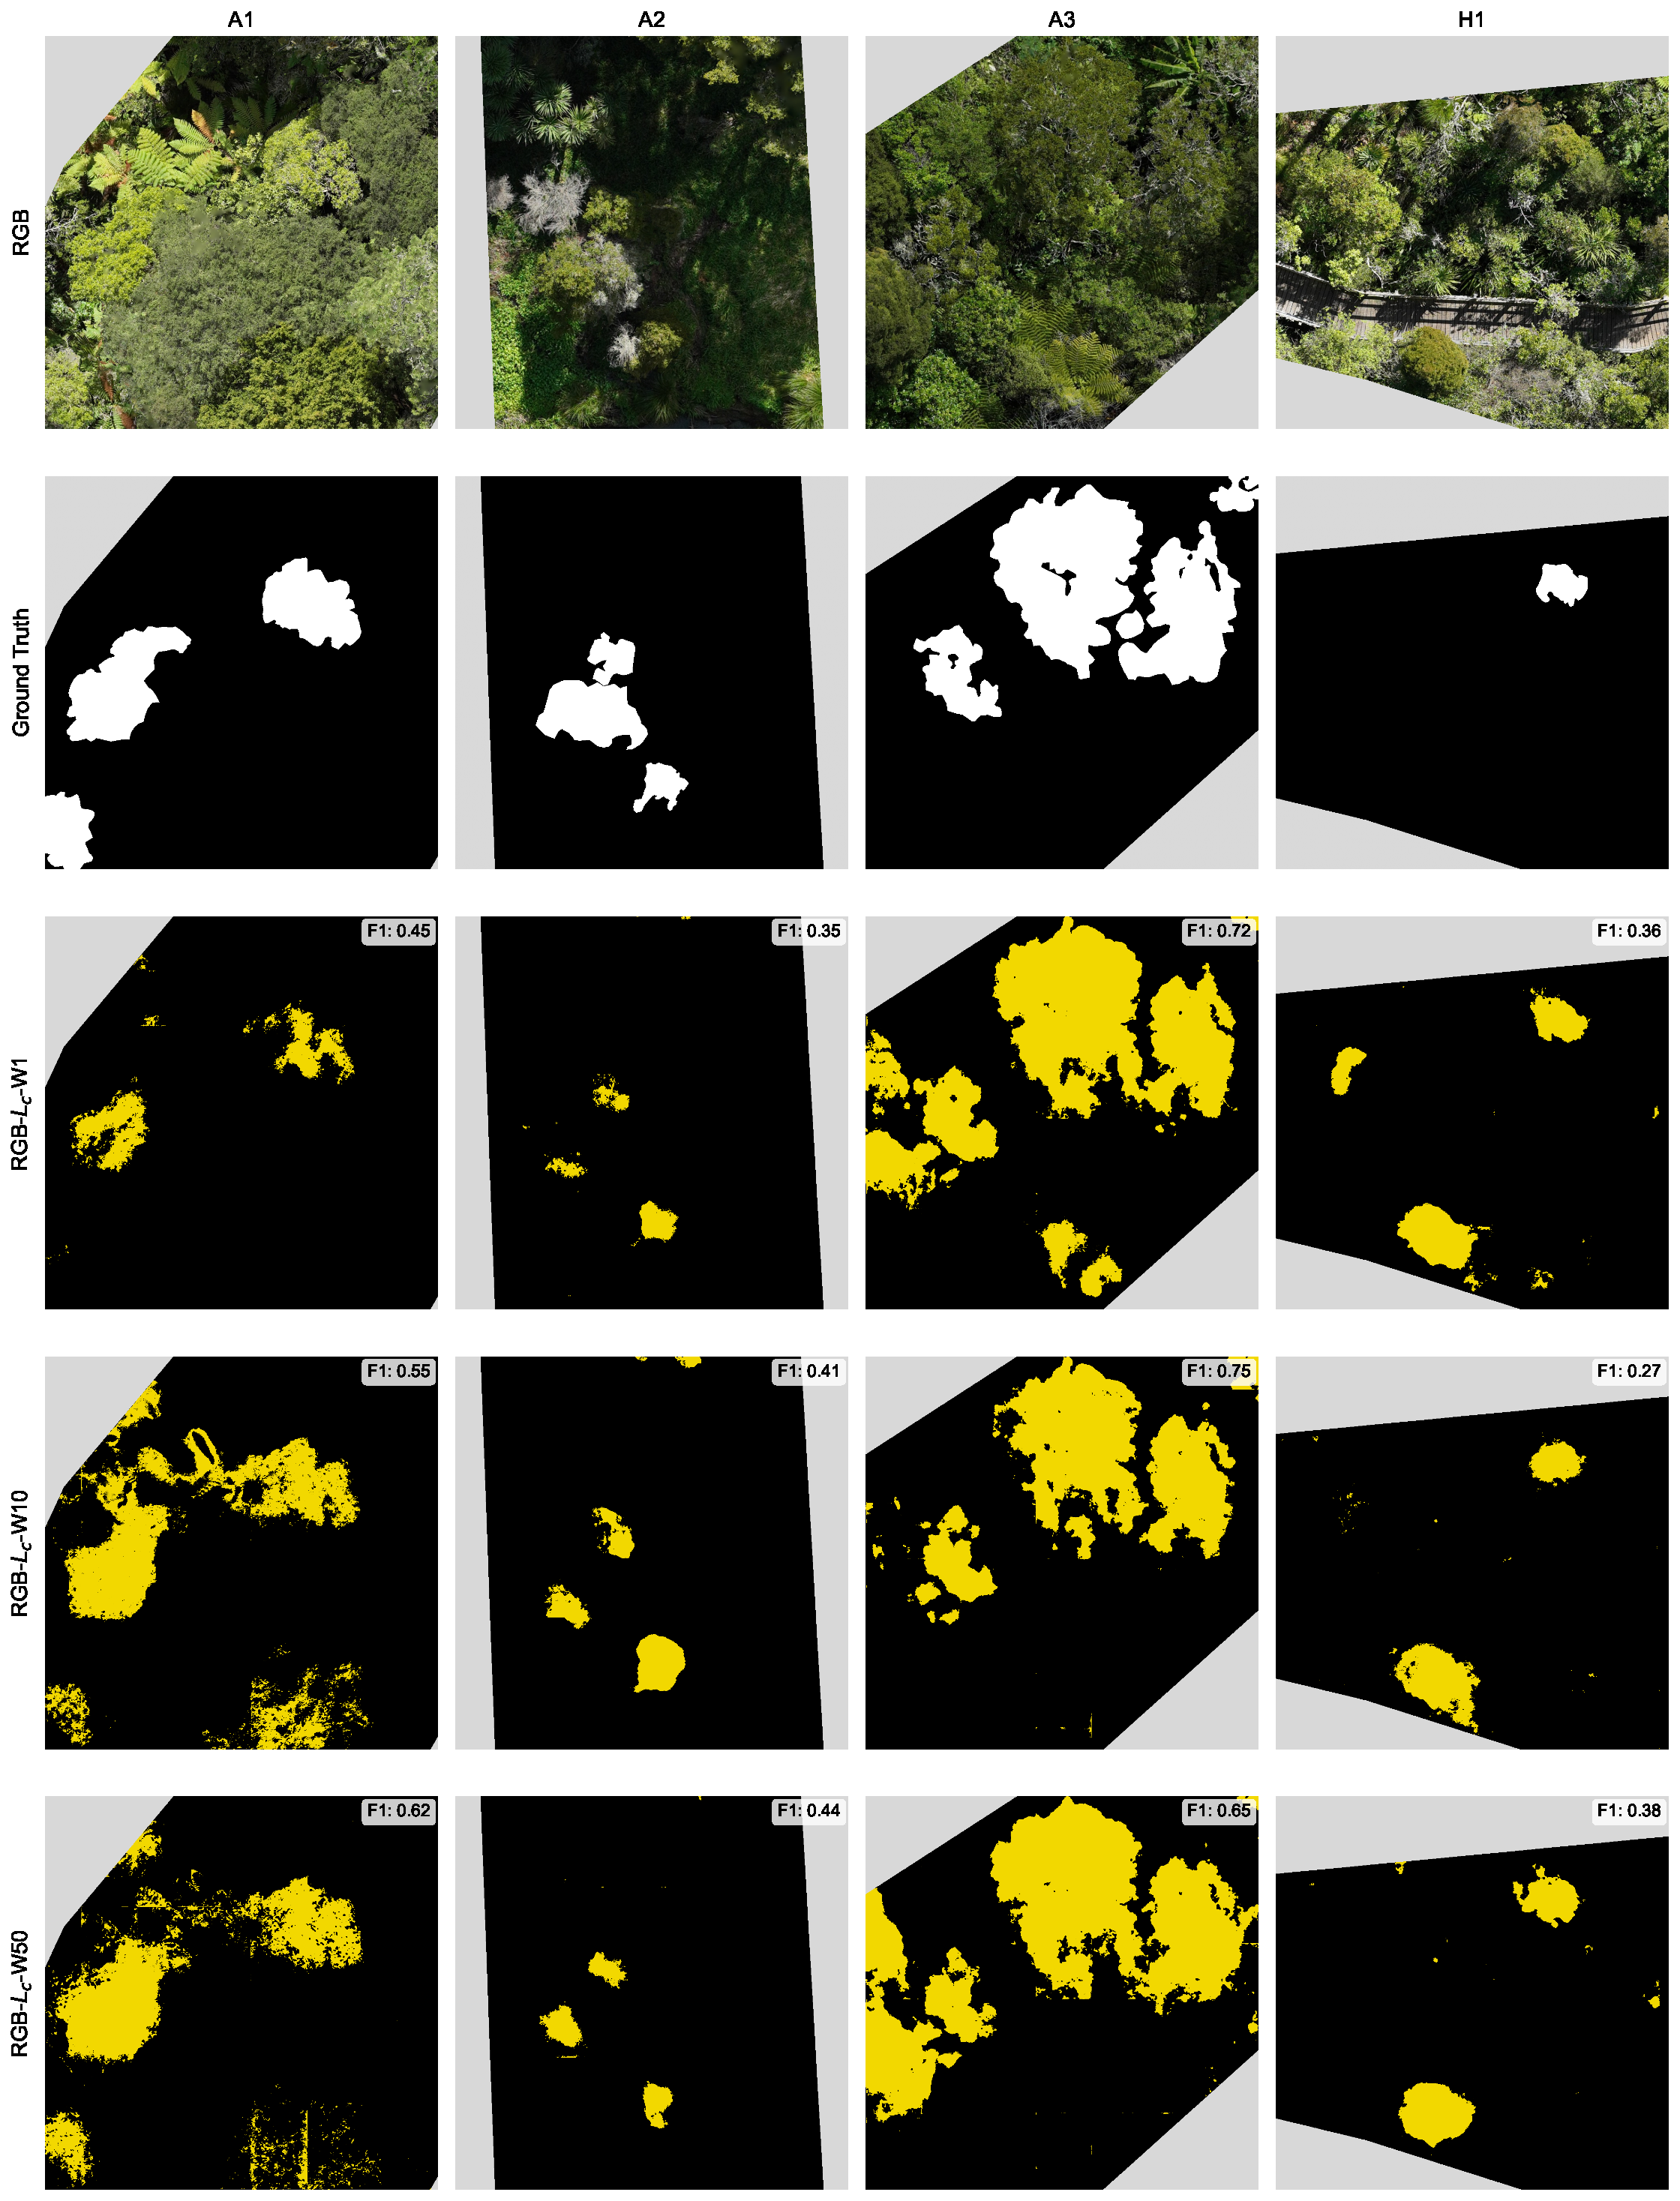
\includegraphics[keepaspectratio]{complete_thesis_files/figure-pdf/cell-27-output-1.pdf}}

}

\caption{\label{sfig-predictions_single_weight_comparison}Predictions
from the single-site models for the test zone for each reserve for a
15x15 m extent. Model configurations are listed on the left; all were
trained with a \hyperref[acronyms_LR]{LR} of 0.02 and weights ranging
from 1, 10 to 50. For example RGB-\(L_{c}\)-W50 reads as: ``model
trained on RGB bands using \hyperref[acronyms_WBCE_D]{\(L_{c}\)} with a
weight of 50''.}

\end{sfig}%

\begin{stbl}[H]

\caption{\label{stbl-multi_site_all}The performance metrics from all
model configurations trained on the multi-site dataset, sorted by F1
score.}

\centering{

\begin{longtable*}[]{@{}
  >{\raggedright\arraybackslash}p{(\linewidth - 12\tabcolsep) * \real{0.2708}}
  >{\raggedright\arraybackslash}p{(\linewidth - 12\tabcolsep) * \real{0.1250}}
  >{\raggedright\arraybackslash}p{(\linewidth - 12\tabcolsep) * \real{0.1667}}
  >{\raggedright\arraybackslash}p{(\linewidth - 12\tabcolsep) * \real{0.1042}}
  >{\raggedright\arraybackslash}p{(\linewidth - 12\tabcolsep) * \real{0.1042}}
  >{\raggedright\arraybackslash}p{(\linewidth - 12\tabcolsep) * \real{0.1250}}
  >{\raggedright\arraybackslash}p{(\linewidth - 12\tabcolsep) * \real{0.1042}}@{}}
\toprule\noalign{}
\begin{minipage}[b]{\linewidth}\raggedright
Bands
\end{minipage} & \begin{minipage}[b]{\linewidth}\raggedright
Loss
\end{minipage} & \begin{minipage}[b]{\linewidth}\raggedright
Weight
\end{minipage} & \begin{minipage}[b]{\linewidth}\raggedright
F1
\end{minipage} & \begin{minipage}[b]{\linewidth}\raggedright
IoU
\end{minipage} & \begin{minipage}[b]{\linewidth}\raggedright
Prec
\end{minipage} & \begin{minipage}[b]{\linewidth}\raggedright
Rec
\end{minipage} \\
\midrule\noalign{}
\endhead
\bottomrule\noalign{}
\endlastfoot
RGB & \hyperref[acronyms_WBCE_D]{\(L_{c}\)} & 50 & 0.51 & 0.34 & 0.39 &
0.72 \\
RGB & \hyperref[acronyms_DICE]{\(L_{Dice}\)} & 1 & 0.50 & 0.33 & 0.45 &
0.56 \\
RGB & \hyperref[acronyms_WBCE_D]{\(L_{c}\)} & 10 & 0.45 & 0.29 & 0.31 &
0.81 \\
MS\(_{rel}\) & \hyperref[acronyms_WBCE_D]{\(L_{c}\)} & 50 & 0.35 & 0.22
& 0.23 & 0.75 \\
MS\(_{rel}\) & \hyperref[acronyms_WBCE_D]{\(L_{c}\)} & 10 & 0.30 & 0.18
& 0.27 & 0.34 \\
IND\(_{abs}\) & \hyperref[acronyms_WBCE_D]{\(L_{c}\)} & 10 & 0.22 & 0.12
& 0.23 & 0.20 \\
IND\(_{abs}\) & \hyperref[acronyms_WBCE_D]{\(L_{c}\)} & 50 & 0.19 & 0.10
& 0.12 & 0.52 \\
MS\(_{rel}\) & \hyperref[acronyms_DICE]{\(L_{Dice}\)} & 1 & 0.16 & 0.09
& 0.44 & 0.10 \\
MS\(_{abs}\) & \hyperref[acronyms_WBCE_D]{\(L_{c}\)} & 50 & 0.16 & 0.09
& 0.17 & 0.15 \\
MS+IND\(_{abs}\) & \hyperref[acronyms_DICE]{\(L_{Dice}\)} & 1 & 0.16 &
0.09 & 0.11 & 0.31 \\
MS+IND\(_{abs}\) & \hyperref[acronyms_WBCE_D]{\(L_{c}\)} & 50 & 0.15 &
0.08 & 0.15 & 0.16 \\
IND\(_{abs}\) & \hyperref[acronyms_DICE]{\(L_{Dice}\)} & 1 & 0.15 & 0.08
& 0.09 & 0.47 \\
MS+IND\(_{abs}\) & \hyperref[acronyms_WBCE_D]{\(L_{c}\)} & 10 & 0.14 &
0.08 & 0.25 & 0.10 \\
MS\(_{abs}\) & \hyperref[acronyms_WBCE_D]{\(L_{c}\)} & 10 & 0.14 & 0.08
& 0.20 & 0.11 \\
MS\(_{abs}\) & \hyperref[acronyms_DICE]{\(L_{Dice}\)} & 1 & 0.09 & 0.05
& 0.19 & 0.06 \\
\end{longtable*}

}

\end{stbl}%

\newpage{}

\chapter*{Appendix C: Reference
Materials}\label{appendix-c-reference-materials}
\addcontentsline{toc}{chapter}{Appendix C: Reference Materials}

\section*{Use of generative Artificial
Intelligence}\label{use-of-generative-artificial-intelligence}

Throughout this Thesis, various AI tools were used to support literature
research, data analysis and the writing process. Any output generated by
generative AI tools was critically evaluated and edited by myself to
ensure accuracy, coherence, and alignment with the scientific content of
the thesis. It was treated as a highly efficient assistant for small
well-defined tasks, whose outputs were considered potentially wrong
until verified and adjusted by myself. The following sections provide a
detailed account of the specific AI tools used and how they have been
applied.

\subsection*{\texorpdfstring{\href{https://github.com/features/copilot}{GitHub
Copilot}}{GitHub Copilot}}\label{github-copilot}

GitHub Copilot was used both in the data analysis and writing process.
It was set to auto mode, so the underlying model was automatically
selected to best suit the given prompt. Available models include:

\begin{figure}

\begin{minipage}{0.38\linewidth}
~\end{minipage}%
%
\begin{minipage}{0.23\linewidth}
\pandocbounded{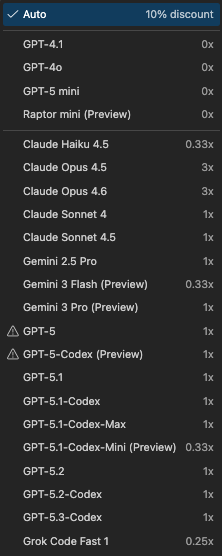
\includegraphics[keepaspectratio]{../2_1_figures/annex/github_copilot.png}}\end{minipage}%
%
\begin{minipage}{0.38\linewidth}
~\end{minipage}%

\end{figure}%

In the data analysis process, it was used to generate code snippets for
data processing, visualisation, and analysis, and to navigate through my
code space to identify relevant code sections within the convoluted
U-Net module. Any provided code was thoroughly tested, adjusted where
needed, and data visualised to ensure it worked as intended and produced
accurate outputs.

In the writing process, personally created bullet points were discussed
to point out potentially missing arguments or adjust placement under
subsections. Furthermore, it was used to check grammar and spelling,
suggest synonyms, and, in some cases, improve sentence structure and
phrasing.

Finally, given the nature of this thesis which was written and formatted
using the Markdown language \href{https://quarto.org/}{Quarto}, Github
Copilot was also used to help with formatting and to generate code
snippets for specific formatting needs (e.g.~tables, figures, or
specific layout requirements).

\subsection*{\texorpdfstring{\href{https://scite.ai/home}{Scite}}{Scite}}\label{scite}

Scite was connected to my Zotero library and used as a tool to point me
to original sources within my own library. No text generated by Scite
was used.

\subsection*{\texorpdfstring{\href{https://www.deepl.com/en/translator}{DeepL}}{DeepL}}\label{deepl}

Sentences with arguments from studies were translated to German with
\href{https://www.deepl.com/en/translator}{DeepL} and paraphrased by
myself in a mix of English and German words. These hybrid sentences were
then translated back to English with
\href{https://www.deepl.com/en/translator}{DeepL} and further adjusted
if needed. This mainly included exchanging words with synonyms.

\subsection*{Microsoft Copilot and
ChatGPT}\label{microsoft-copilot-and-chatgpt}

ChatGPT and Copilot were used to generate search terms to scan scholarly
databases for literature research.

\subsection*{\texorpdfstring{\href{https://languagetool.org/paraphrasing-tool}{LanguageTool}
paraphrasing
tool}{LanguageTool paraphrasing tool}}\label{languagetool-paraphrasing-tool}

The rephrasing tool was scarcely used on single sentences to improve
wording and sentence structure.

\section*{Reprint Permissions}\label{reprint-permissions}

\pandocbounded{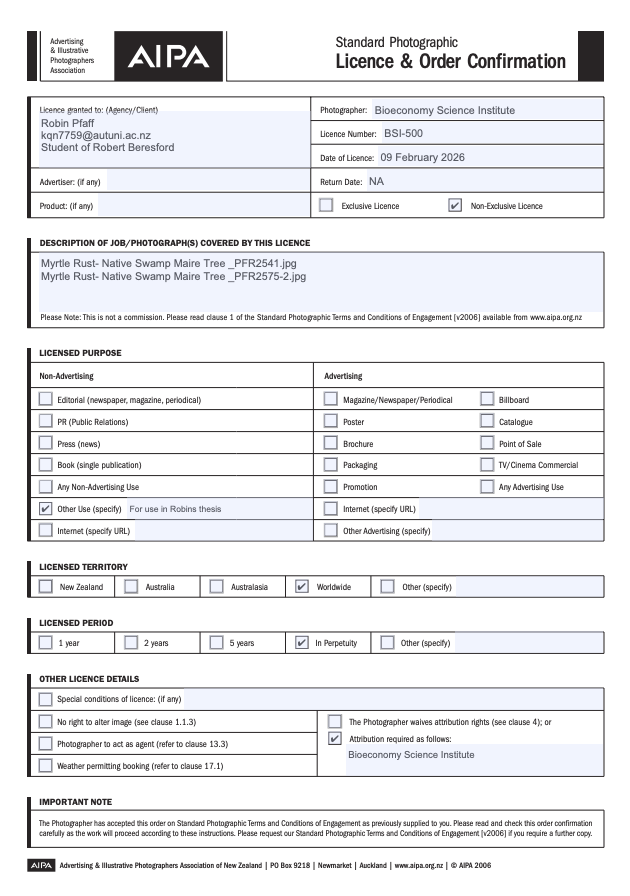
\includegraphics[keepaspectratio]{../2_1_figures/annex/BSI_permission.png}}

Reprint permission for Figure~\ref{fig-pustules}.




\end{document}
